\chapter{Results}
\label{cap:Results}

Many samples collected by different studies have shown that Twitter is a scale-free\cite{Kwak:2010,Borondo:2016}, small-world\cite{Java:2007} and have community structure\cite{Java:2007,Wang2012,Darmon2013,Darmon2015,Bedi2016}. However, most of theses samples were collected with the intention to identify global characteristics of Twitter and most of them represent  networks formed by the follow relation only. In this work, we adopted a local view of Twitter, by considering sub-graphs of Twitter local to a user, i.e. ego networks. This ego networks are multilayer networks where each layer corresponds to a distinct type of interaction. 

We do not just study the layer corresponding the follow relation a user has with other people in Twitter, but also the layers derived from other three important and dynamic interactions: like, retweet and mention. Specifically, we want to know if these layers of ego networks tend to be scale-free, if they can be considered small-world graphs and if their vertices tend to cluster into communities. Besides, we are interested in comparing the layers according to these properties and to investigate how similar they are in terms of their vertex and edge sets. Because we collected our data from the Twitter lists that the ego is linked to, we also took the opportunity to evaluate the behavior of egos in relation to other users who are also on the lists. We provide some research questions to guide our  investigation and present in the following subsections the answers to these questions obtained experimentally from our dataset.

%%%%%%%%%%%%%%%%%%%%%%%%%%%%%%%%%%%%%%%%%%%%%% 
%%%%%%%%%%%%%%%%%%%%%%%%%%%%%%%%%%%%%%%%%%%%%% Nodes

\begin{figure}[h!tb]
    \centering
    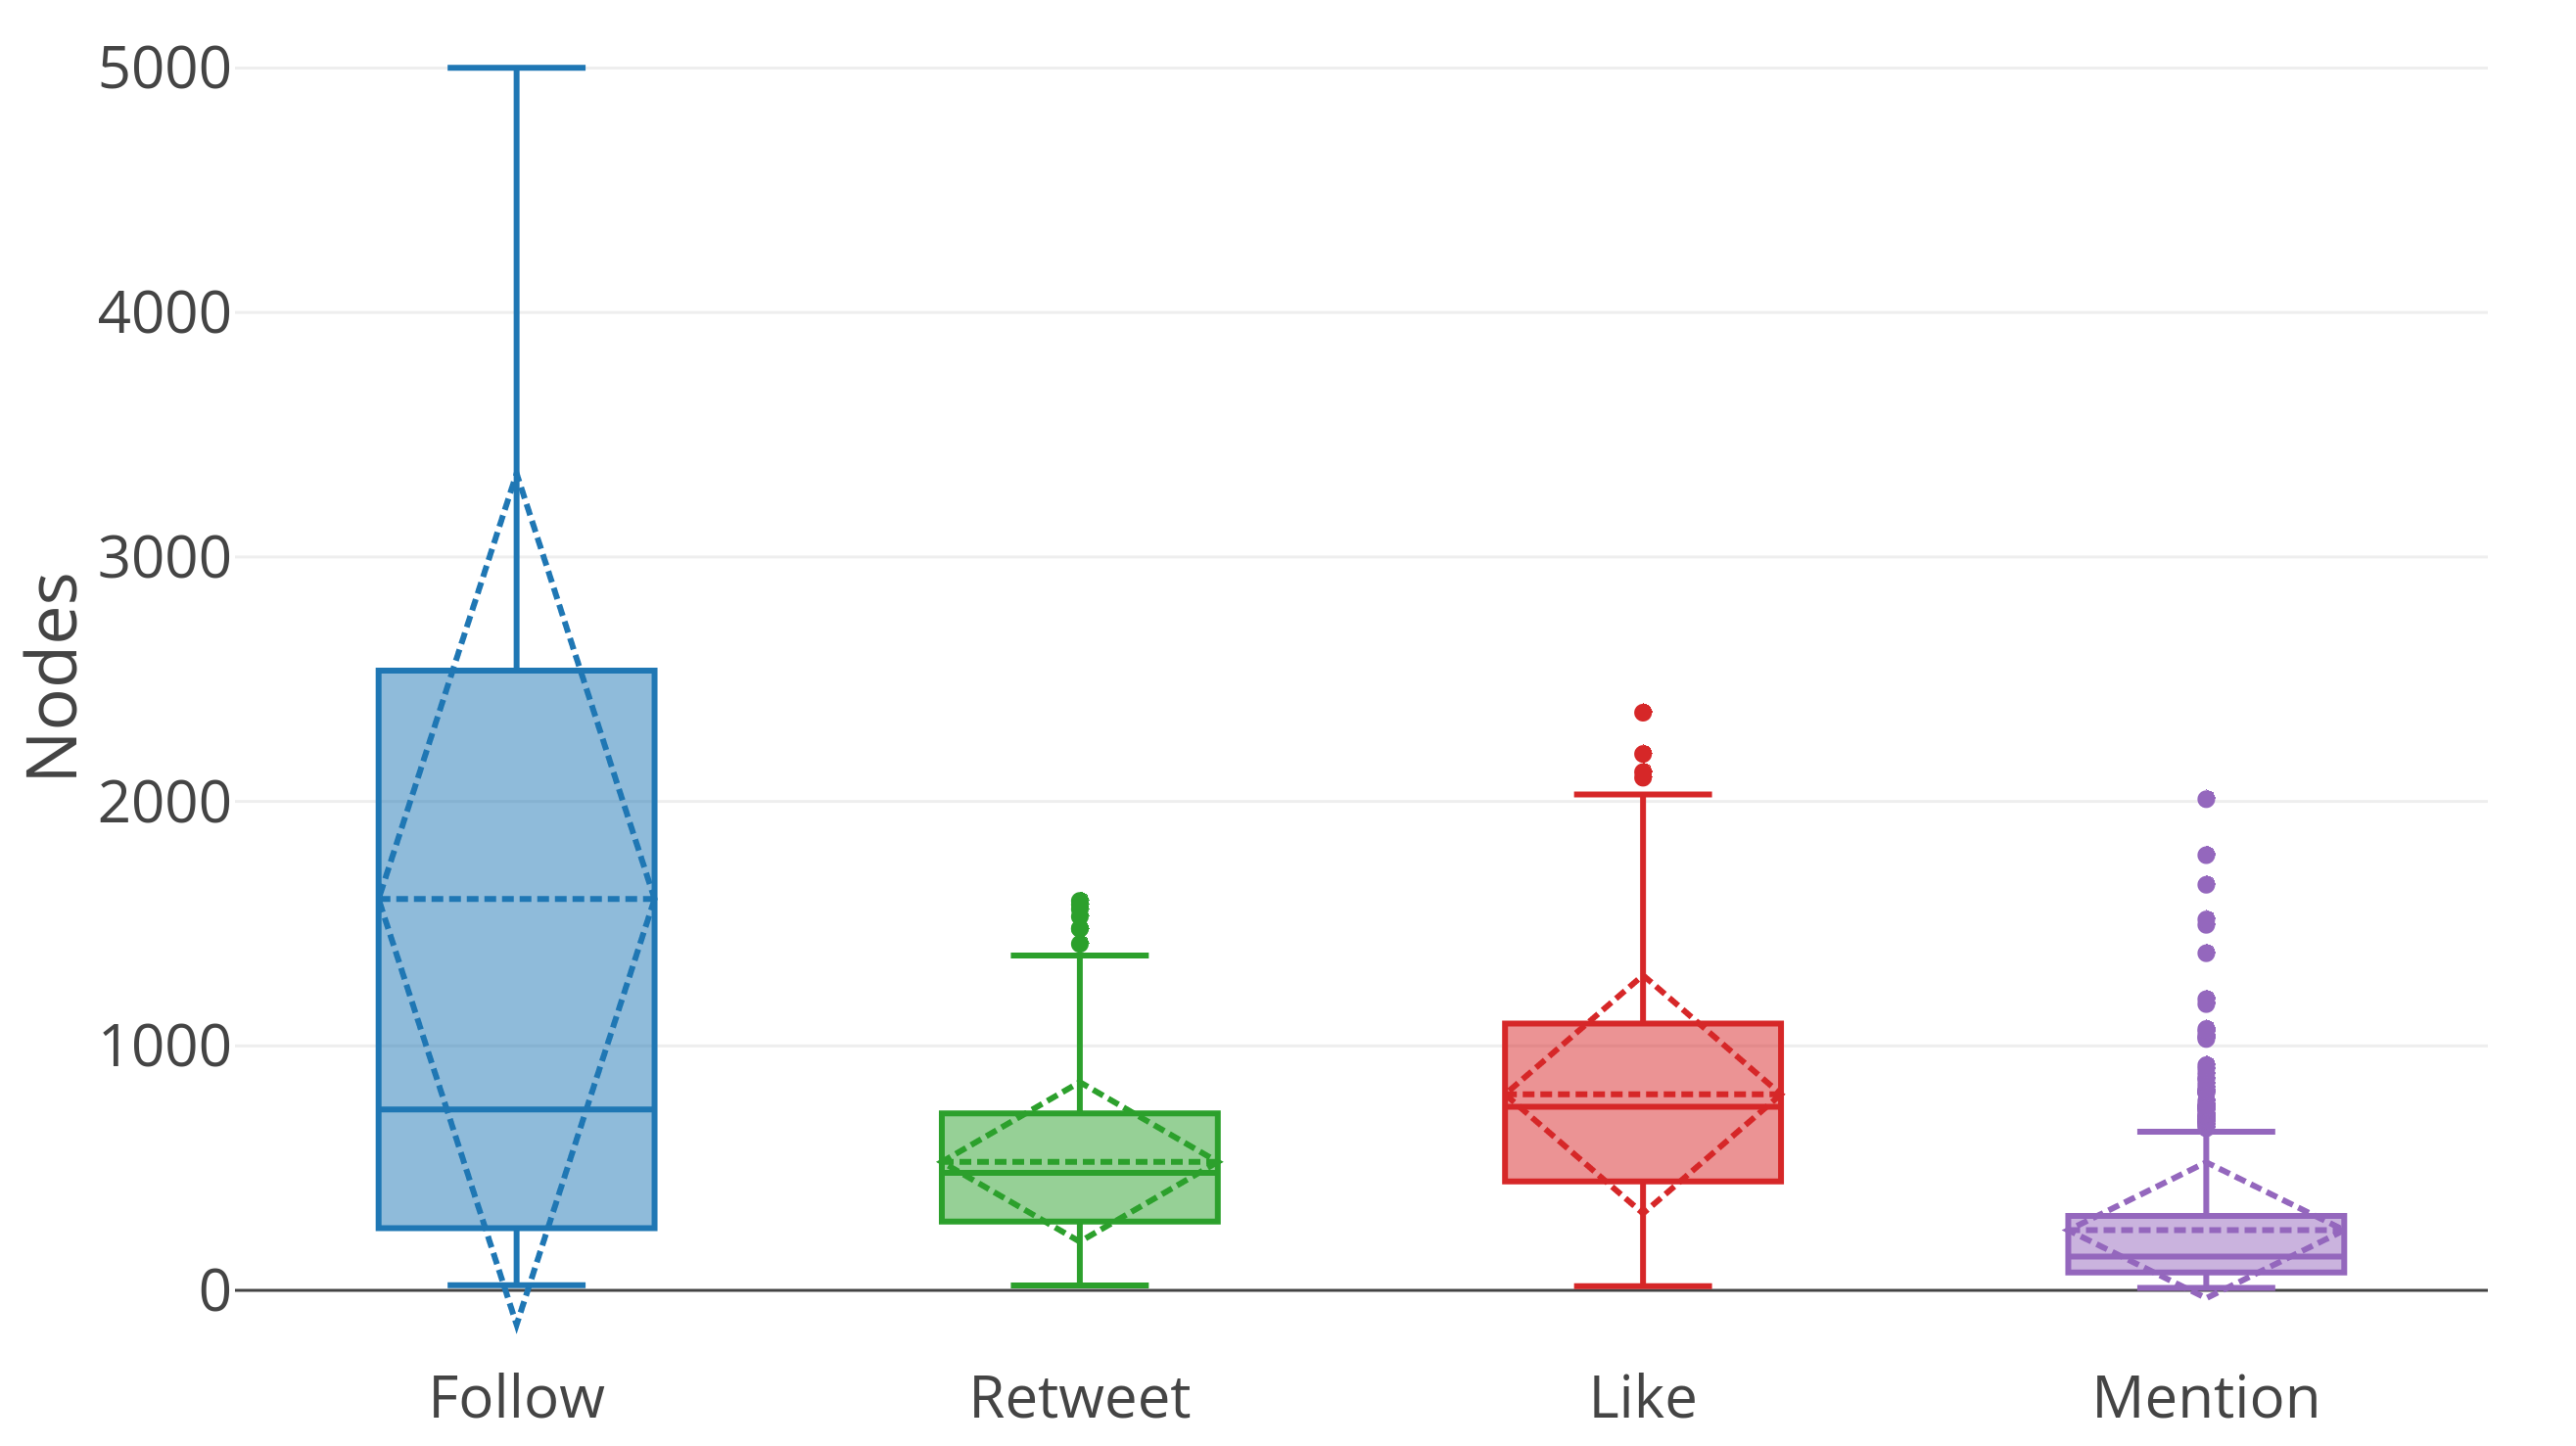
\includegraphics[width=1\textwidth]{fig/net_struct/number_of_nodes.png}
    \caption{Number of vertices in each layer.}
    \label{fig:net_struct_nodes}
\end{figure}


\begin{table}[h!tb]
    \renewcommand{\arraystretch}{1.3}
    \caption{Mean number of vertices, standard deviation, median, the minimum number and the maximum number of vertices found in each layer for the 500 ego networks.}
    \label{tab:numVertices}
    \centering
    \scriptsize
    \setlength\tabcolsep{6pt} % default value: 6pt
    \begin{tabular}{|c|c|c|c|c|c|}
    \hline
        {\bf Layer} &   {\bf Mean}  &   {\bf Stdv}  &   {\bf Median} & {\bf Min}  &   {\bf Max}  \\  \hline \hline
        Follow      &   1,600.77    &   1,742.74    &       740     &       21      &       5,001   \\  \hline
        Retweet    &   525.47      &   326.72      &       480.5   &       20      &       1,593   \\  \hline
        Like       &   801.84      &   487.79      &       750.5   &       17      &       2,363   \\  \hline
        Mention    &   246.08      &   278.31      &       138     &       10      &       2,009   \\  \hline \hline 
    \end{tabular}
\end{table}

\section{How the sizes of the ego networks vary among layers?}
\label{sec:net_structure}


We want to investigate the distribution of sizes of both number of vertices and number of edges in the four layers. Fig. \ref{fig:net_struct_nodes} present box plots of the distribution of the number of vertices in each layer of the 500 ego networks considered. Fig. \ref{fig:net_struct_edges} shows the distribution of the number of edges and Fig. \ref{fig:net_struct_density} shows the distribution of the density of edges in each layer. Tables \ref{tab:numVertices}, \ref{tab:numEdges} and \ref{tab:density} shows some additional information regarding the numbers of vertices, edges and the density of each layer. 

%%%%%%%%%%%%%%%%%%%%%%%%%%%%%%%%%%%%%%%%%%%%%% 
%%%%%%%%%%%%%%%%%%%%%%%%%%%%%%%%%%%%%%%%%%%%%% Edges

\begin{figure}[h!tb]
    \centering
    \begin{subfigure}
        \centering
        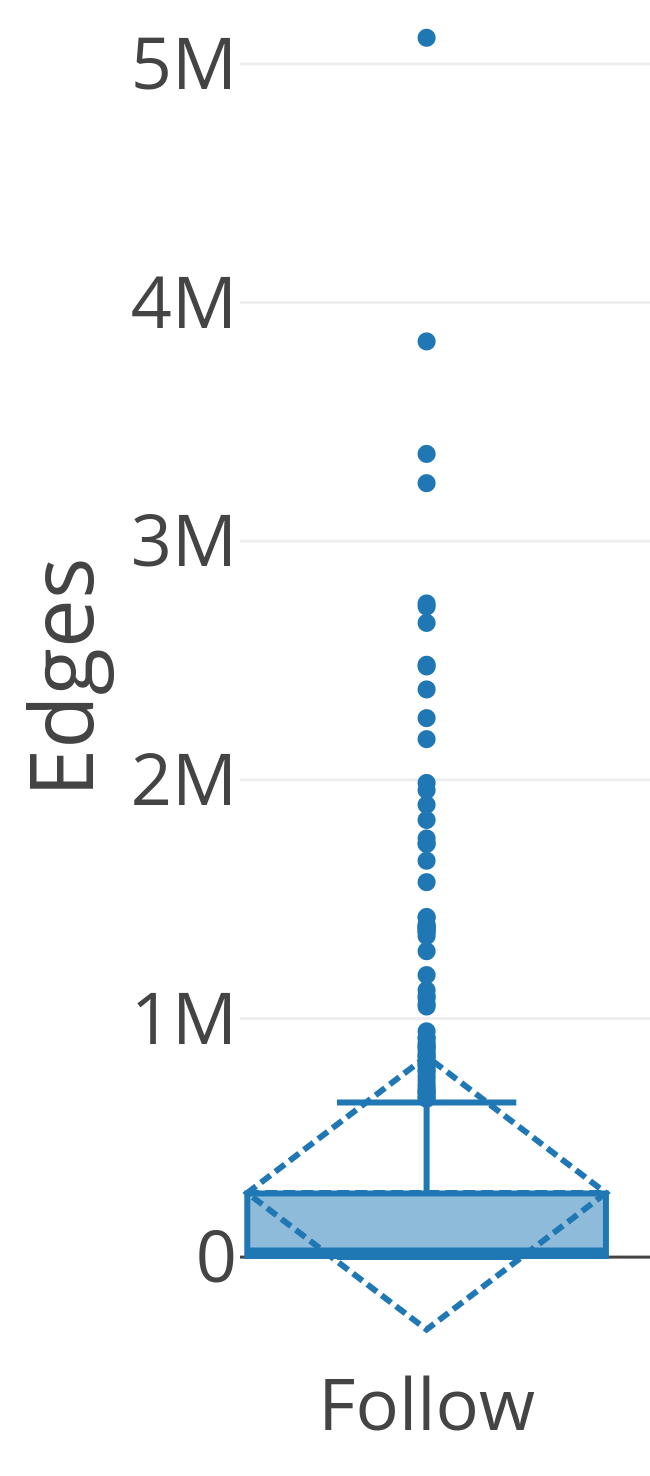
\includegraphics[width=0.23\textwidth]{fig/net_struct/number_edges_follow.png}
        %\caption{Follow}
    \end{subfigure}%
    ~ 
    \begin{subfigure}
        \centering
        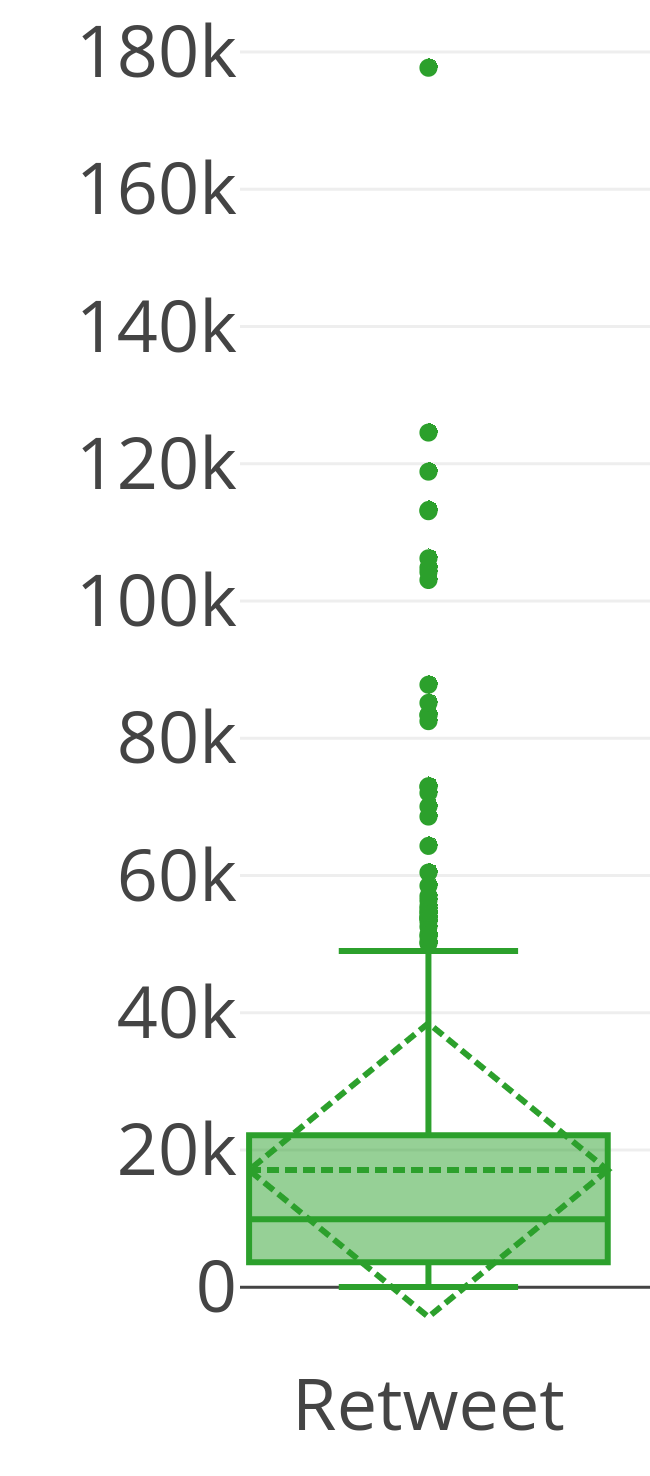
\includegraphics[width=0.23\textwidth]{fig/net_struct/number_edges_retweets.png}
        %\caption{Retweets}
    \end{subfigure}
    ~
    \begin{subfigure}
        \centering
        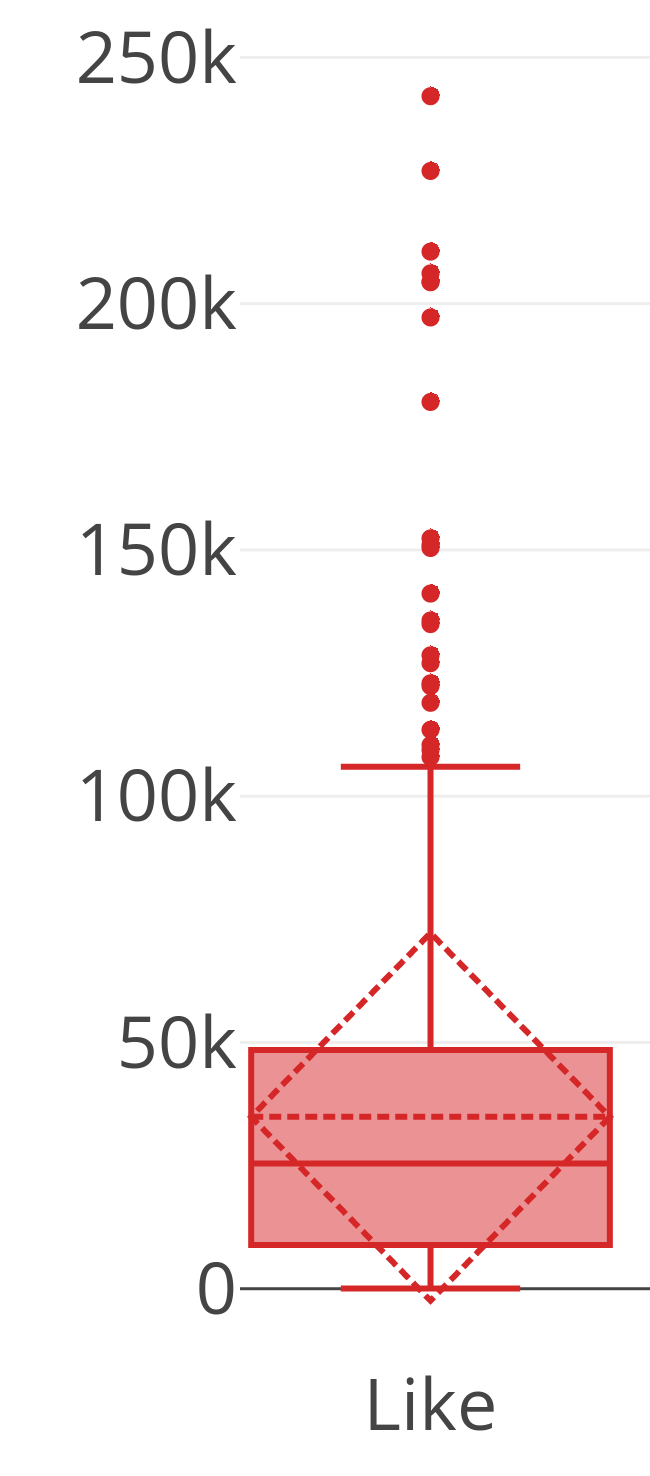
\includegraphics[width=0.23\textwidth]{fig/net_struct/number_edges_likes.png}
        %\caption{Likes}
    \end{subfigure}%
    ~ 
    \begin{subfigure}
        \centering
        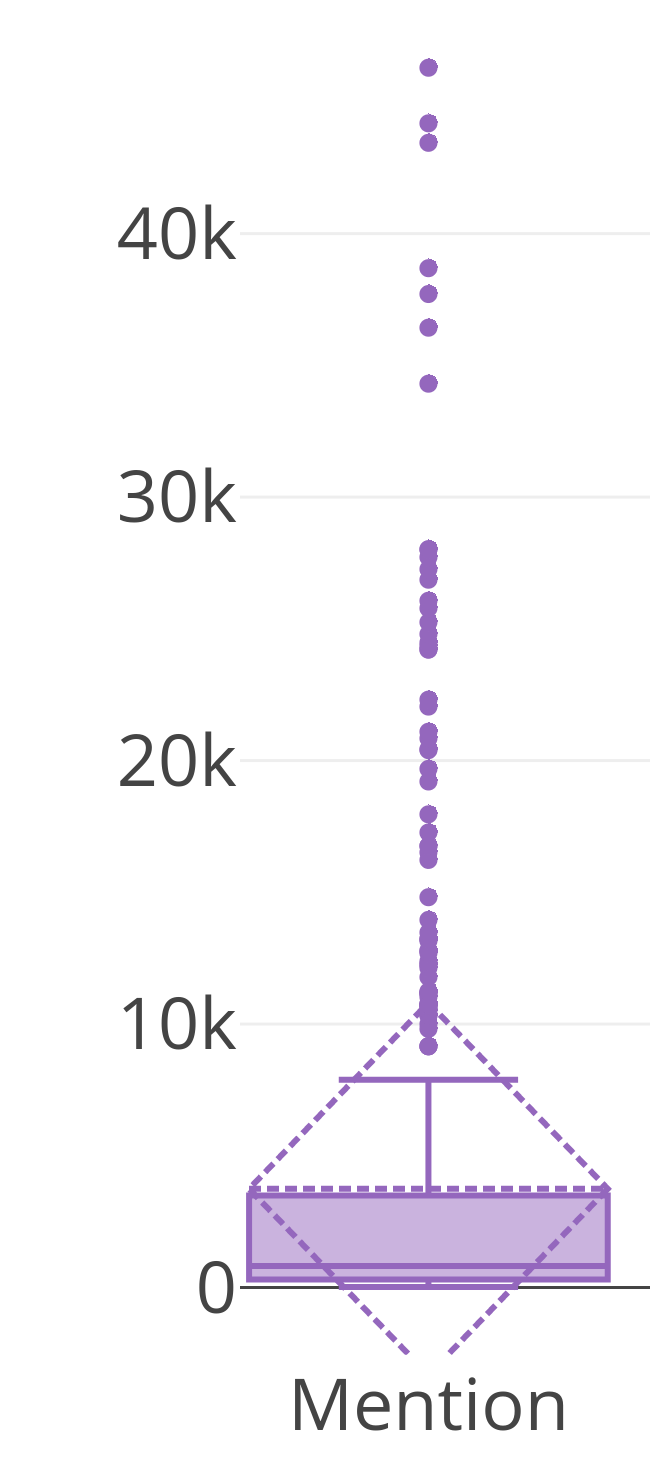
\includegraphics[width=0.23\textwidth]{fig/net_struct/number_edges_mentions.png}
        %\caption{Mentions}
    \end{subfigure}
    \caption{Number of edges in each layer.}
    \label{fig:net_struct_edges}
\end{figure}

\begin{table}[h!tb]
    \renewcommand{\arraystretch}{1.3}
    \caption{Mean number of edges, standard deviation, median, the minimum number and the maximum number of edges found in each layer for the 500 ego networks.}
    \label{tab:numEdges}
    \centering
    \scriptsize
    \setlength\tabcolsep{6pt} % default value: 6pt
        \begin{tabular}{|c|c|c|c|c|c|}
        \hline
        {\bf Layer} &   {\bf Mean}  &   {\bf Stdv}  &   {\bf Median}  &   {\bf Min}  &   {\bf Max}  \\ \hline \hline
        Follow      &   268,773.31  &   573,100.38  &   28,109.5    &       66      &   5,109,659   \\  \hline
        Retweet    &   17,073.12   &   21,423.85   &   9,917.5     &       31      &   177,702     \\  \hline
        Like       &   34,898.04   &   37,356.02   &   25,404.0    &       39      &   242,118     \\  \hline
        Mention    &   3,745.34    &   7,070.79    &   817         &       17      &   46,296      \\  \hline\hline 
    \end{tabular}
\end{table}

The number of vertices varies very much among egos for a same layer. The follow layer being the one with more intense variation. As shown in Fig. \ref{fig:net_struct_nodes}, half of the egos in our sample have up to 740 followees (alters), but the number of followees in the other half of the egos vary enormously, up to the limit of 5.000 followees. In the other three layers there is also a great variation, as can be seen by the standard deviation values in Fig. \ref{tab:numVertices}, but it is not so high as in the case of the follow layer. 

It is also interesting to notice that the number of alters in the mention layers is usually less than in all the other layers for all egos. This seems to reflect the nature of this interaction. A mention is a direct communication between two users via a tweet. It implies in a certain acquaintance between the sender and the receiver of the tweet. This naturally implies in a restriction on the number of alters. The same does not necessary occurs with like and retweet layers, because a user may retweet or like a tweet independently if she knows or not its author.


%%%%%%%%%%%%%%%%%%%%%%%%%%%%%%%%%%%%%%%%%%%%%% 
%%%%%%%%%%%%%%%%%%%%%%%%%%%%%%%%%%%%%%%%%%%%%% Density

\begin{figure}[h!tb]
    \centering
    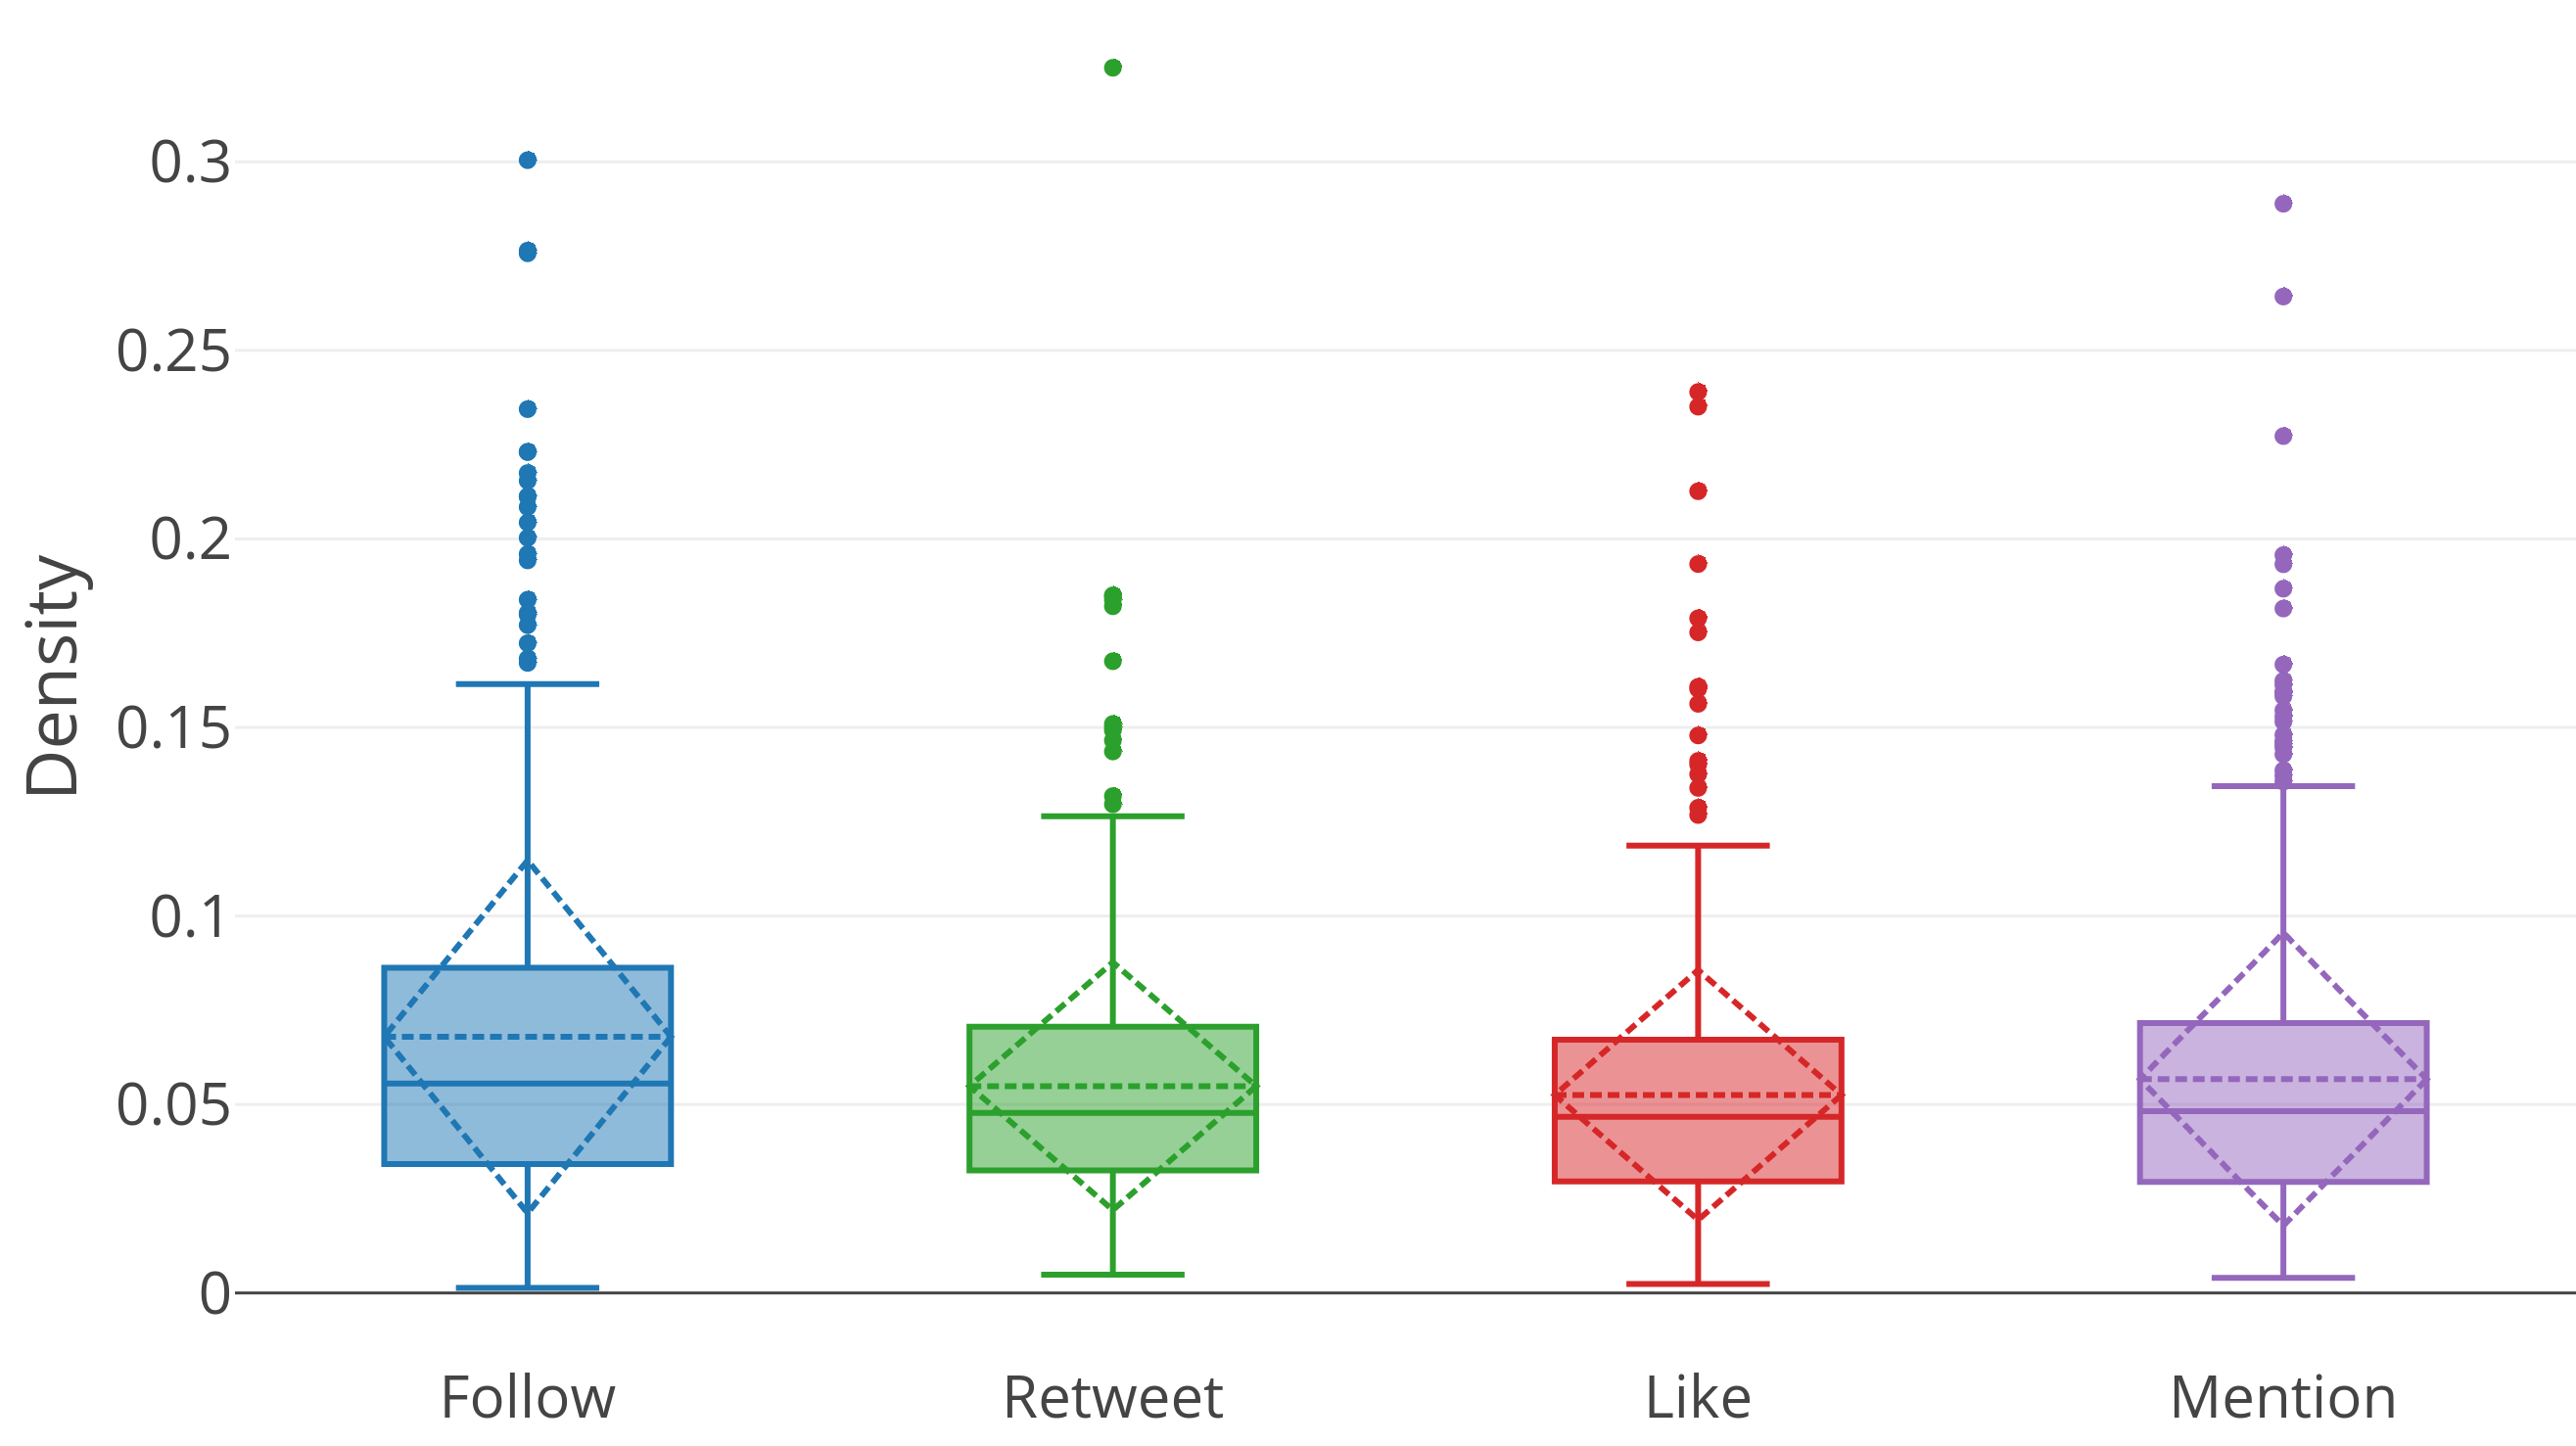
\includegraphics[width=1\textwidth]{fig/net_struct/density.png}
    \caption{Density of edges in each layer.}
    \label{fig:net_struct_density}
\end{figure}

\begin{table}[h!tb]
    \renewcommand{\arraystretch}{1.3}
    \caption{Mean, standard deviation, median, the minimum and the maximum value of density found in each layer for the 500 ego networks.}
    \label{tab:density}
    \centering
    \scriptsize
    \setlength\tabcolsep{6pt} % default value: 6pt
    \begin{tabular}{|c|c|c|c|c|c|}
        \hline
        {\bf Layer} &   {\bf Mean}  & {\bf Stdv}  & {\bf Median} & {\bf Min} & {\bf Max}  \\  \hline \hline
        Follow     &    0.0680    &   0.0468  &     0.0556      &  0.0013   &  0.3005\\  \hline
        Retweet    &    0.0548    &   0.0329  &     0.0478      &  0.0048   &  0.3250\\  \hline
        Like       &    0.0525    &   0.0331  &     0.0467      &  0.0024   &  0.2390\\  \hline
        Mention    &    0.0567    &   0.0388  &     0.0482      &  0.0040   &  0.2889\\  \hline \hline 
    \end{tabular}
\end{table}

Fig. \ref{fig:net_struct_edges}  shows also  a great variation on the number of edges in all layers. However, when observing the density distribution of all this layers in Fig. \ref{fig:net_struct_density} we can see that independent of the so large differences on the number of edges and vertices among egos in all layers, the distributions of edges in the graphs are equally very sparse. We have very few edges in all layers of all ego networks compared to the possible number of edges that could exist (i.e $|\{e\}\cup A_e^i|(|\{e\}\cup A_e^i|-1)$ for a layer $i$). In fact, 75\% of the egos have edge density inferior to 0.1 in all layers. This implies that most alters interact only with a small fraction of the same layer members, including the ego and the other alters. In other words, the intersections of the alter set of an ego  $e$ and the alter sets of her alters are very small in all layers.

\begin{figure}[h!tb]
    \centering
    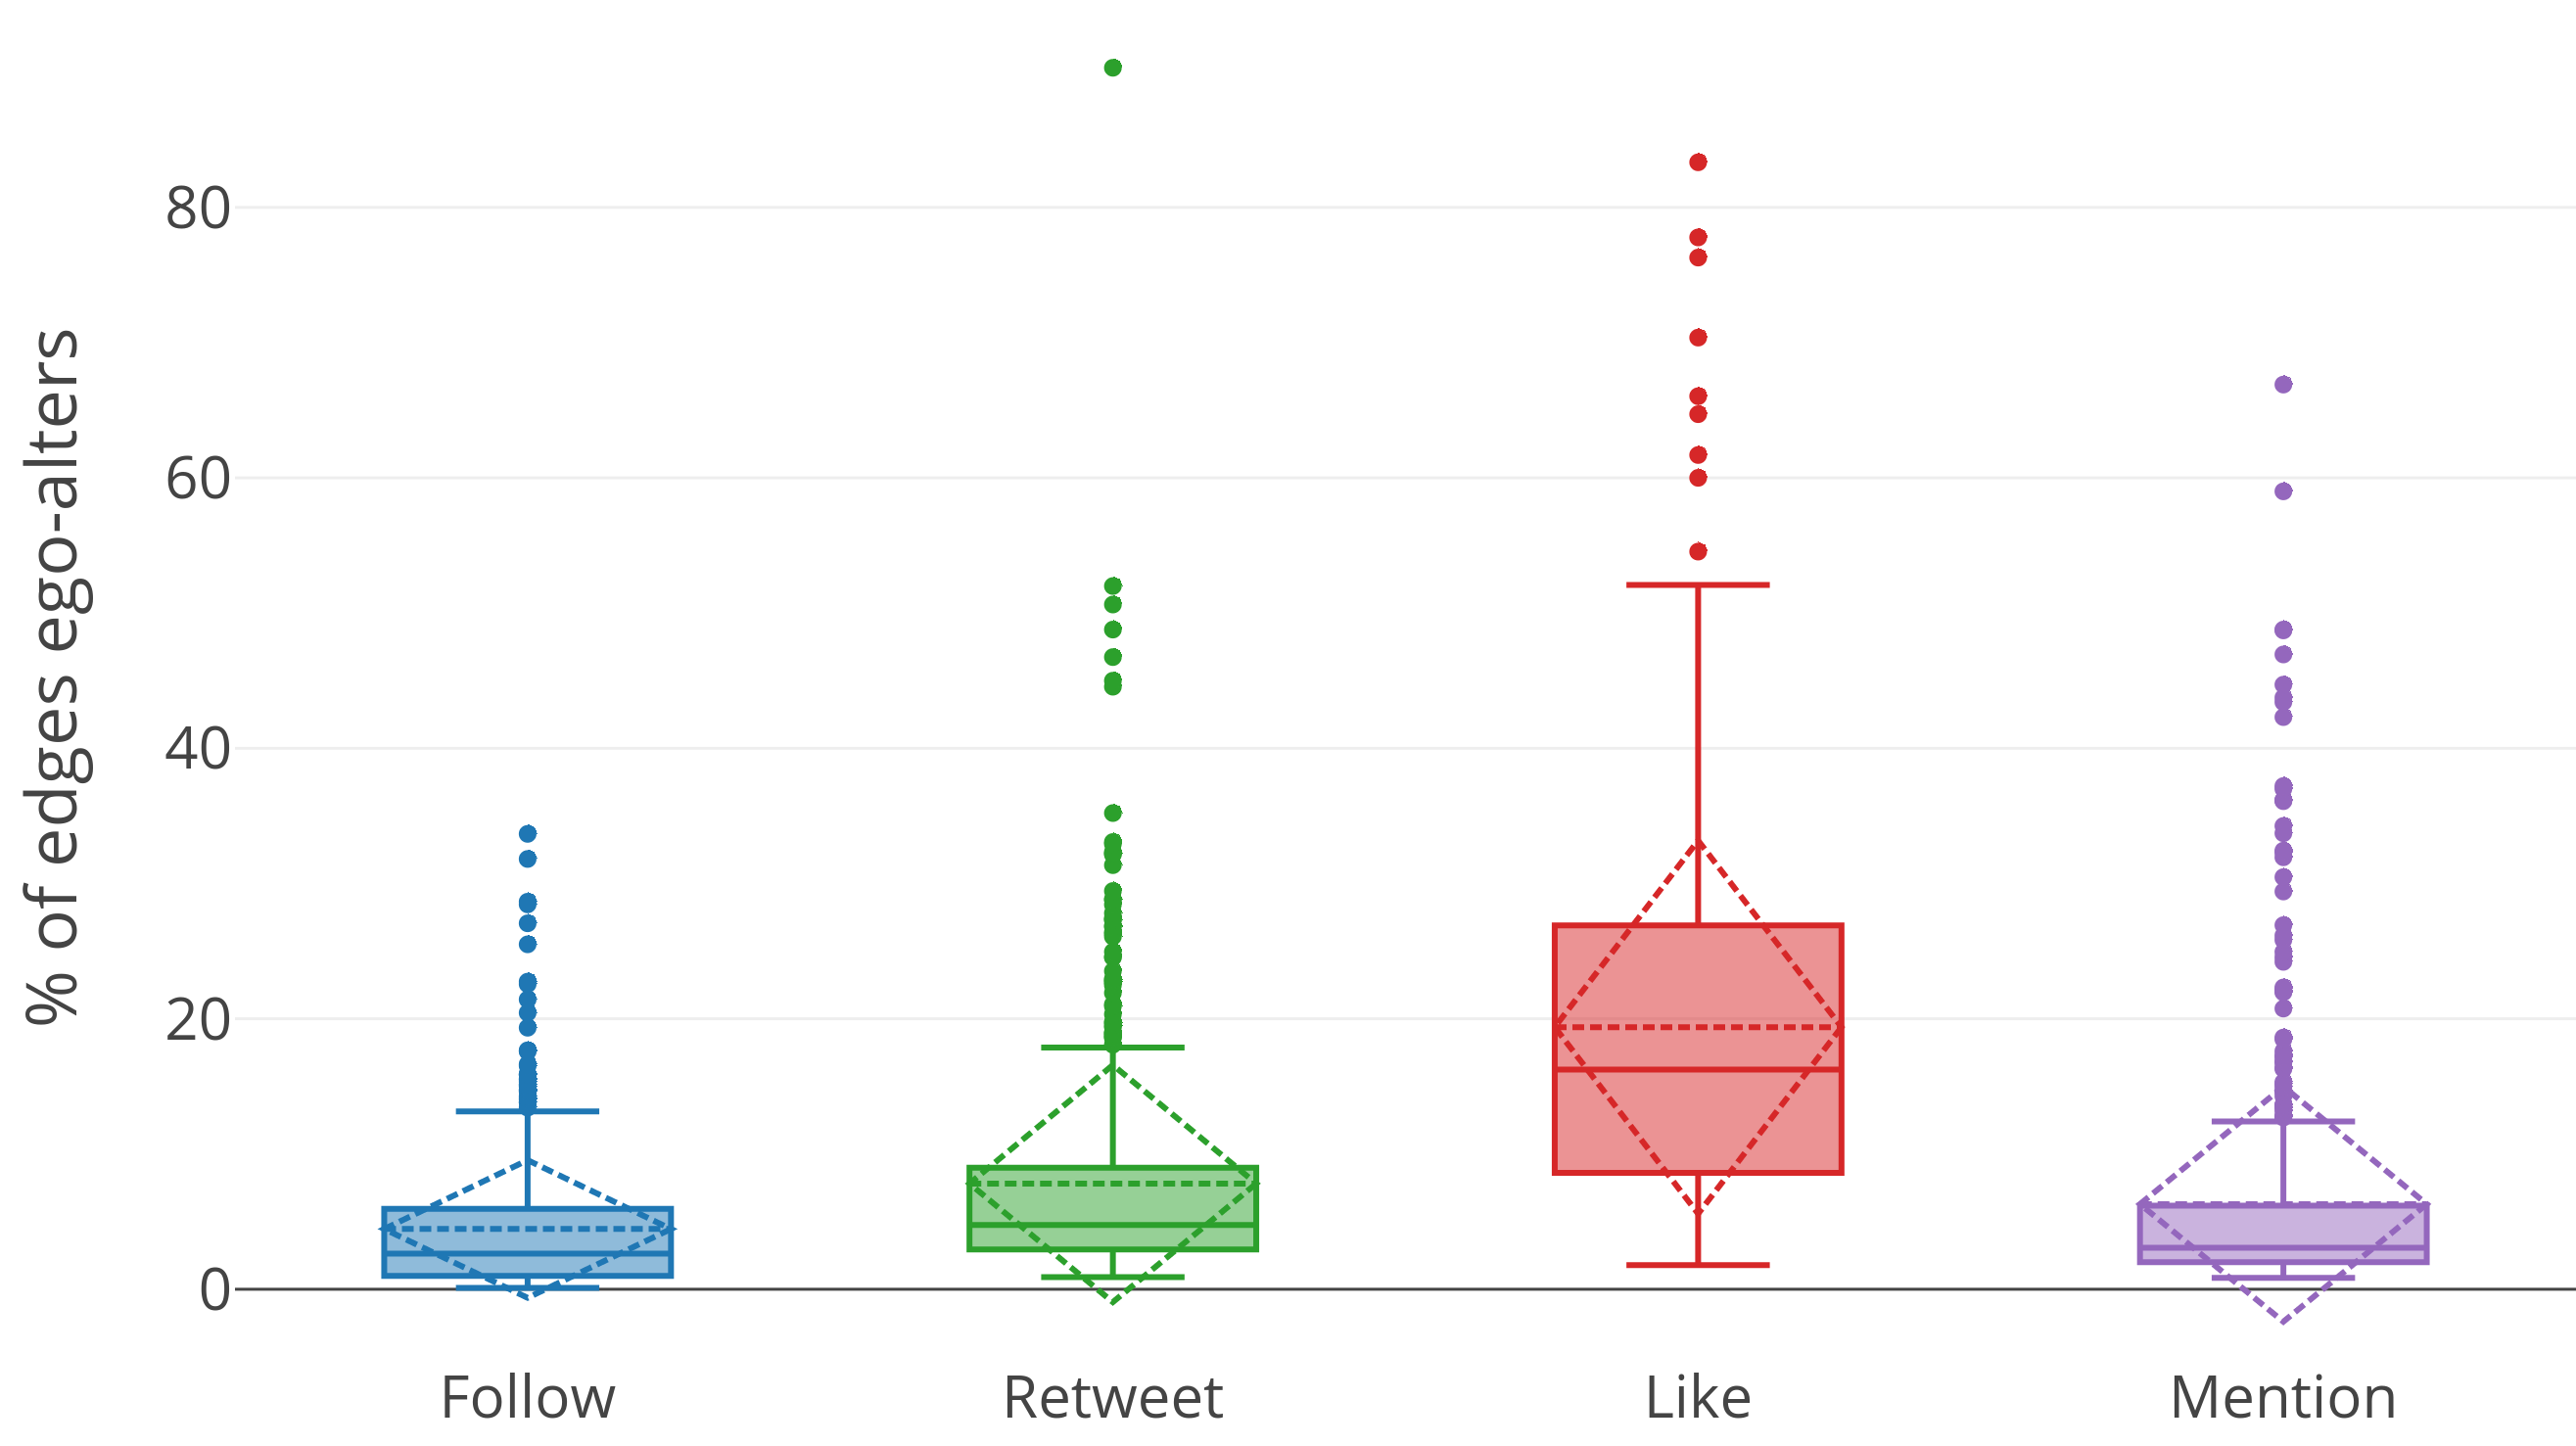
\includegraphics[width=1\textwidth]{fig/net_struct/edges_ego_alters.png}
    \caption{Percentage of edges ego-alters.}
    \label{fig:net_struct_edges_ego_alters}
\end{figure}

As the edge density is low, the number of edges that start from the ego and arrive at the alter is also low, according to the results presented in Fig. \ref{fig:net_struct_edges_ego_alters}. The users with whom the ego interacts also interact with each other or interact back with the ego using the same type of interaction, with almost all ego networks having a number of ego-alters edges less than 20\%. Except is due to the like layer, where the number of ego-alters edges is on average close to 20\%. This result shows that all ego networks are sparse, but among the existing edges there are a significant number of edges that start from the alters and therefore the ego networks are not mostly formed by ego-alters edges.

We also investigated if there is a correlation of the number of alters in different layers for an ego. If the correlation value of the number of egos between two layer of an ego is high, this could be a characteristic of the ego profile, i.e., introspective egos would tend to have a small set of alters in all layers and more communicative egos would have a great number of alters in all layers. However, as Fig. \ref{fig:net_struct_nodes_correlation} shows, we have strong values of the Spearman correlation between the pair of layers (like, retweet) and  (follow, mention) layers; and weak values between (follow, like). There is practically no correlation between the pairs (follow, retweet) and (like, mention); and the (retweet, mention) layers has a moderate negative correlation. Thus, we can conclude that usually a user does not follow a same pattern when interacting with all different types of interaction in Twitter, regarding the number of people she interact with different types of interaction.

\begin{figure}[h!tb]
    \centering
    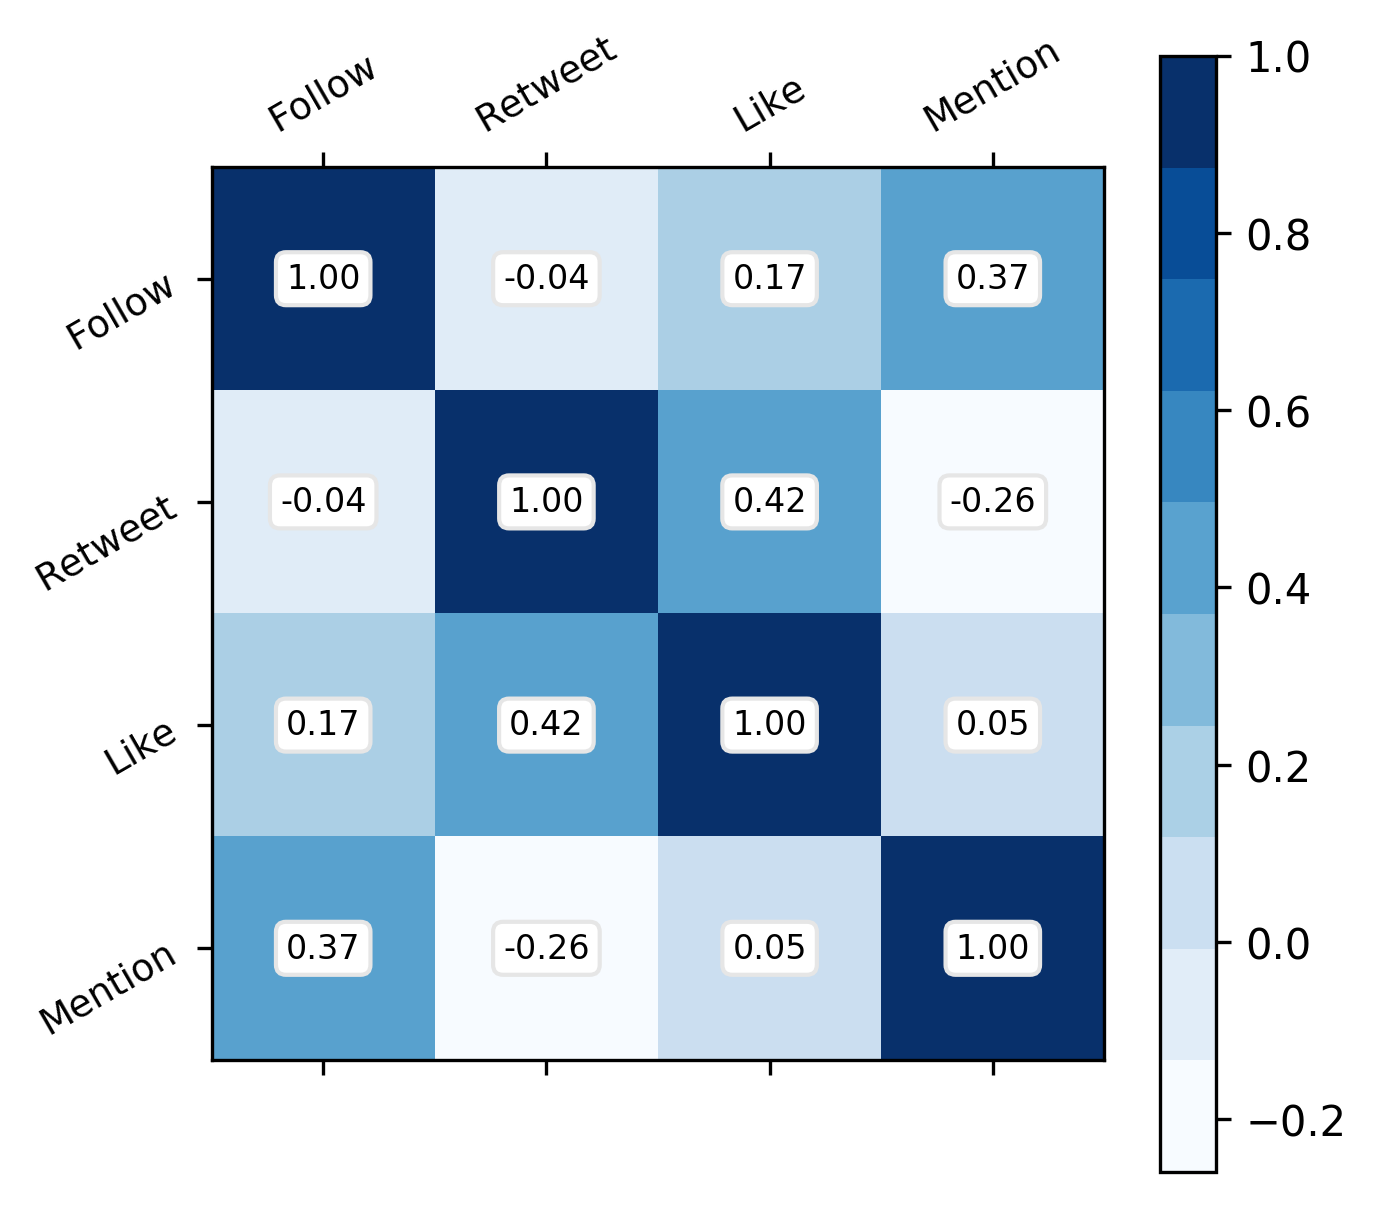
\includegraphics[width=0.8\textwidth]{fig/net_struct/nodes_correlation_spearman.png}
    \caption{Vertices Spearman's Correlation inter-layers.}
    \label{fig:net_struct_nodes_correlation}
\end{figure}

The standard deviation presented in the Tab. \ref{tab:numVertices} reveals that the variation in the size of the retweet and like layers (alters set) is much smaller when compared to the follow and mention networks, which seems to be a pattern in the behavior of users regarding the ability to interact with different alters - there seems to be a tendency for stabilization/saturation in the size of the retweet and like layers. While in the follow and mention layers the size of the set of alters varies greatly from one ego to another, in the retweet and like layers the size of the set seems to converge to a mean value. The results observed in Fig. \ref{fig:net_struct_nodes_correlation} also reinforce the idea that there is a tendency of stabilization in the size of the retweet and like layers because there is a strong correlation between these two layers, and by the convergence in the number of alters.

We also note that there is a moderate correlation between the size of the layers (follow, mention), indicating that the ability to mention distinct alters correlates with the number of users that the ego follows. The higher the number of alter in the follow layer, the greater the number of alters in the mention layer, unlike the results of the correlation between (follow,retweet) and (follow,like) layers, showing that the number of alters in the follow layer has practically no correlation with the number of alters of the retweet layer and a weak correlation with the number of alters of the like layer. 



%%%%%%%%%%%%%%%%%%%%%%%%%%%%%%%%%%%%%%%%%%%%%% 
%%%%%%%%%%%%%%%%%%%%%%%%%%%%%%%%%%%%%%%%%%%%%% Questions
%%%%%%%%%%%%%%%%%%%%%%%%%%%%%%%%%%%%%%%%%%%%%% 
%%%%%%%%%%%%%%%%%%%%%%%%%%%%%%%%%%%%%%%%%%%%%% 
\subsection*{How reciprocal are the relations inside each layer?}
\label{subsec:reciprocity_result}
\begin{figure}[h!tb]
    \centering
    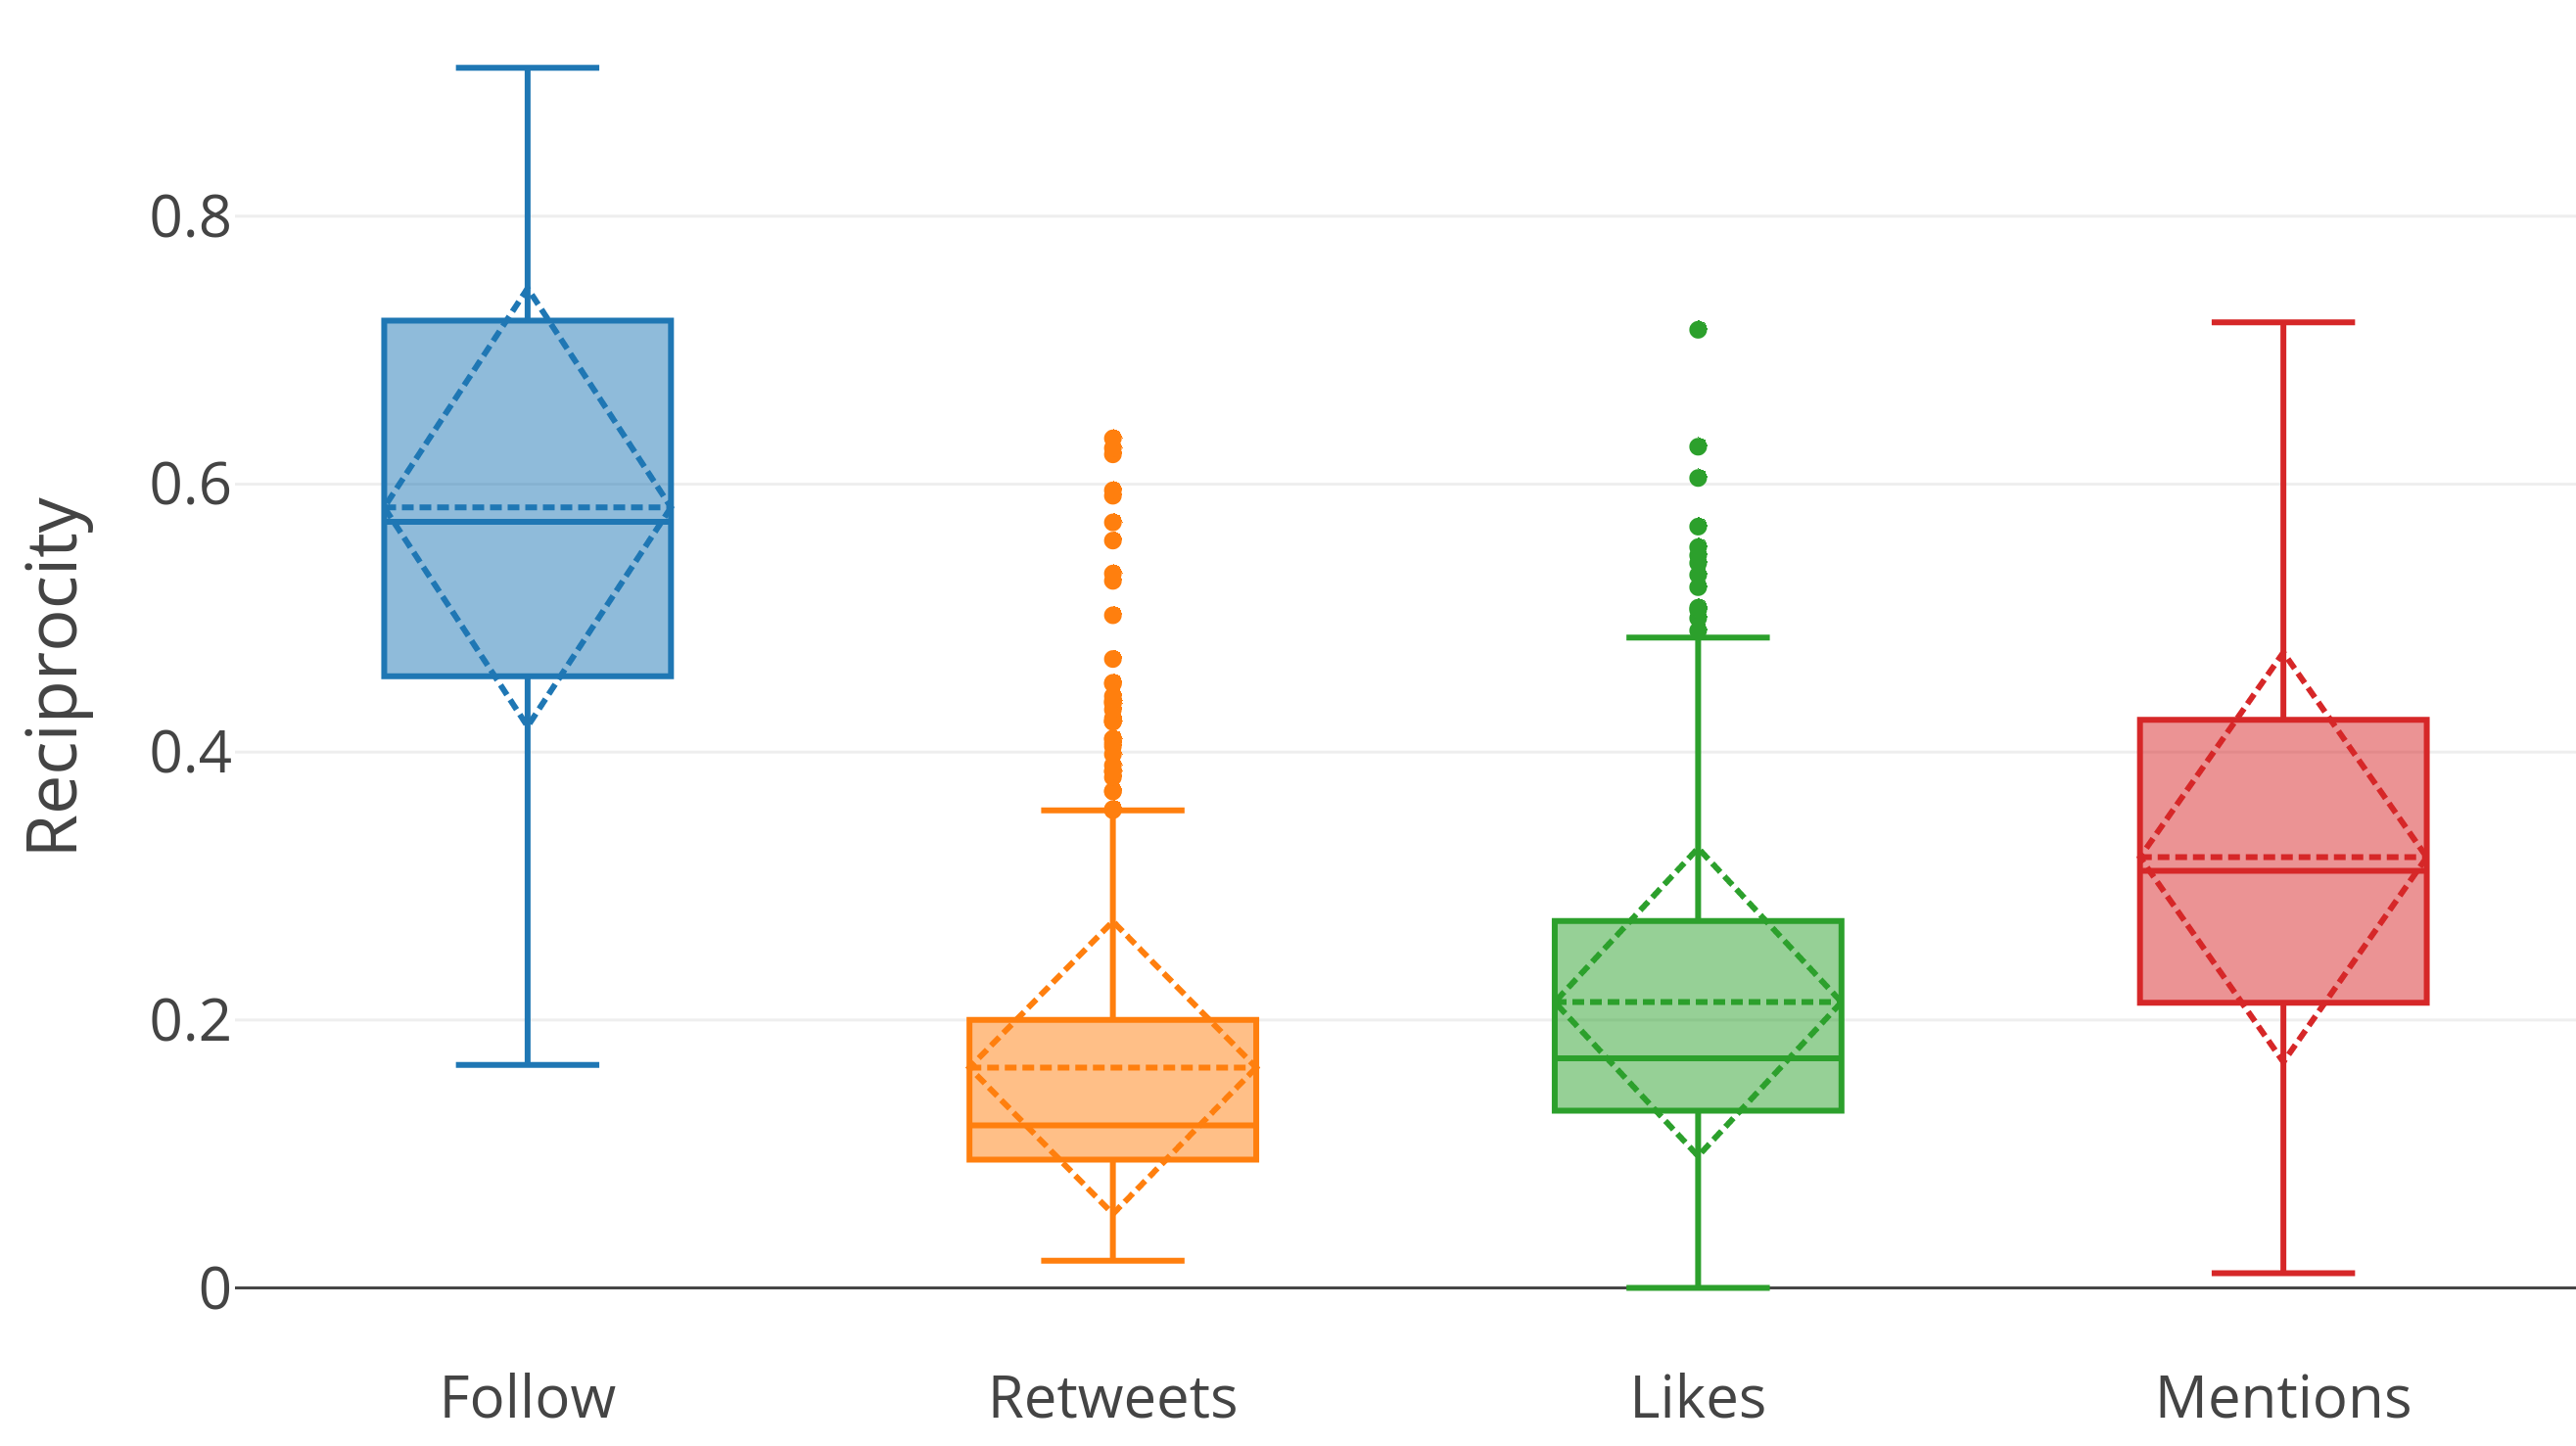
\includegraphics[width=1\textwidth]{fig/net_struct/reciprocity.png}
    \caption{Reciprocity.}
    \label{fig:net_struct_reciprocity}
\end{figure}

Reciprocity evaluates whether interactions between users in a particular layer occur reciprocally, or are predominantly unidirectional interactions, and was computed using Eq. \ref{eq:reciprocity}. The results of reciprocity in multilayer ego networks reveal important differences among layers, as can be seen in Fig \ref{fig:net_struct_reciprocity}. The follow layer has the greatest values. However, Twitter user interface allows a user to see all her followers and to choose to follow back any of them. This may be a great incentive for reciprocity in the follow layer. 

On the other hand, it is interesting to see in the case of dynamic operations as like, follow and mention, how they influence reciprocity. While the first two operations work as endorsements of having read a good tweet and indirectly as endorsement of the writer as a good author, mention tends to imply at least a short term engagement between two users. That is because a mention works as a direct message from one person to the other and a received message tends to induce a response message. Results in the Fig \ref{fig:net_struct_reciprocity} seem to reflect these observations. We can see that reciprocity values for retweet an like layers are similar and small while numbers for the mention layer are comparatively bigger.


\section{How similar are the layers of Twitter multilayer ego networks?}
\label{sec:QuestionSimilarLayers}

In this section we investigate how similar two graphs corresponding to two different layers  of an ego network are. To answer this question, we need to know how similar the vertices set and the edges sets of two distinct layers are. The measure of these similarities reveal two information: a) Is the set of people an ego interacts to with interaction type $x$ similar to the set of people she interacts to with interaction type $y$? b) Interactions between two individuals in one layer repeat in other layers?

%%%%%%%%%%%%%%%%%%%%%%%%%%%%%%%%%%%%%%%%%%%%%% 
%%%%%%%%%%%%%%%%%%%%%%%%%%%%%%%%%%%%%%%%%%%%%% Vertex Overlap
\subsection*{Vertex Overlap}
\label{subsec:vertex_overlap}

\begin{figure}[h!tb]
    \centering
    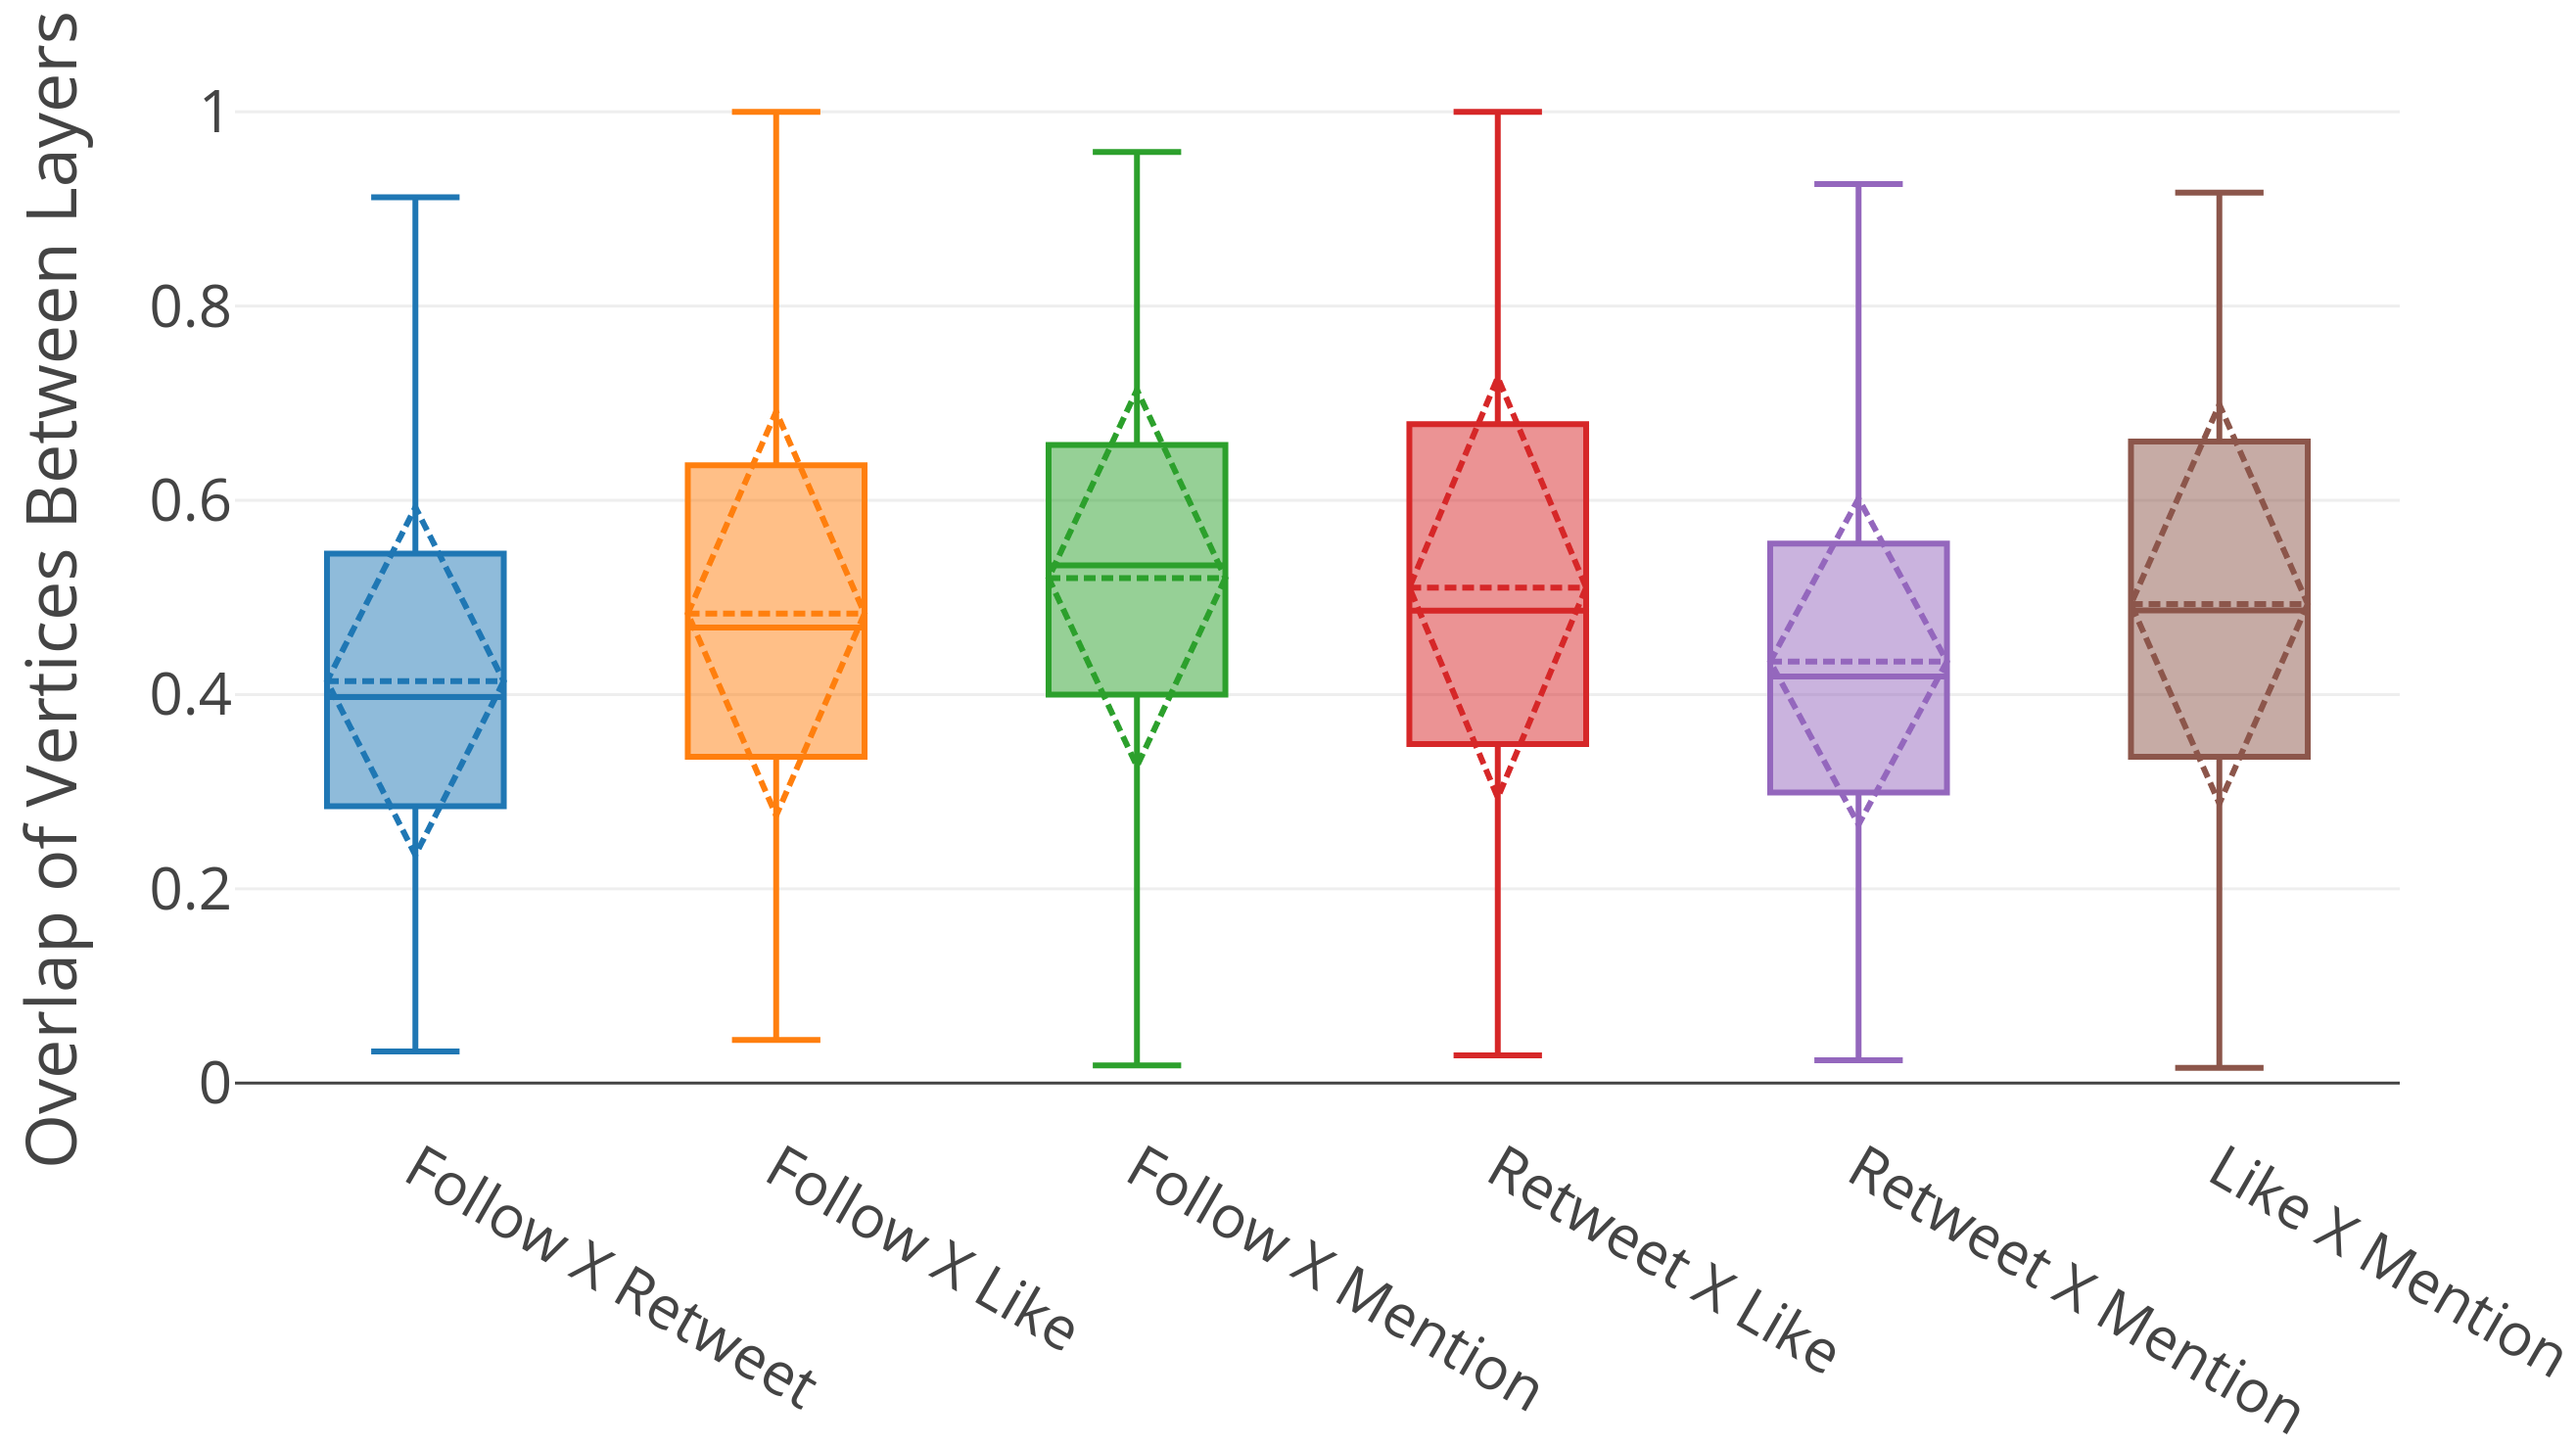
\includegraphics[width=1\textwidth]{fig/net_struct/overlap/overlap_vertices_boxplot.png}
    \caption{Vertex overlap between layers.}
    \label{fig:net_struct_overlap_vertices_boxplot}
\end{figure}

Fig. \ref{fig:net_struct_overlap_vertices_boxplot} shows that there is a great variability of vertex overlap for a given pair of layers, with some egos with almost zero vertex overlap between layers and some with almost 100\% of vertex overlap. However, most egos (those in interquartile)  have some alter overlap between layers. For instance, 50\% of egos have overlap values between 0.2 to almost 0.6 for the pairs (follow, retweet) and (retweet, mention) and 25\% of the egos have vertex overlap superior do 0.6 in these layers. In other pairs, vertex overlap are slightly greater. This means that for about 75\% of egos at least 20\% of their alters in a layer $x$ also occur in layer $y$, for $|A^x| \leq |A^y|$ (according to definition of overlap adopted -- see Eq. \ref{eq:overlap}. It can be seen that the pair (follow, mention) tends to have more vertex overlap values than the other pairs, meaning that people that an ego mentions tend to be her followees. 

Thus, most egos present some overlap among their alters sets belonging to different layers, but the set of vertices are still distinct between pairs of layers, with at least 30\% of the alters in the smaller layer not occurring in the bigger one, in most cases (see the third quartile not reaching 70\% of overlap in any layer). 


%%%%%%%%%%%%%%%%%%%%%%%%%%%%%%%%%%%%%%%%%%%%%% 
%%%%%%%%%%%%%%%%%%%%%%%%%%%%%%%%%%%%%%%%%%%%%% Edge Overlap
\subsection*{Edge Overlap}
\label{subsec:edge_overlap}

\begin{figure}[h!tb]
    \centering
    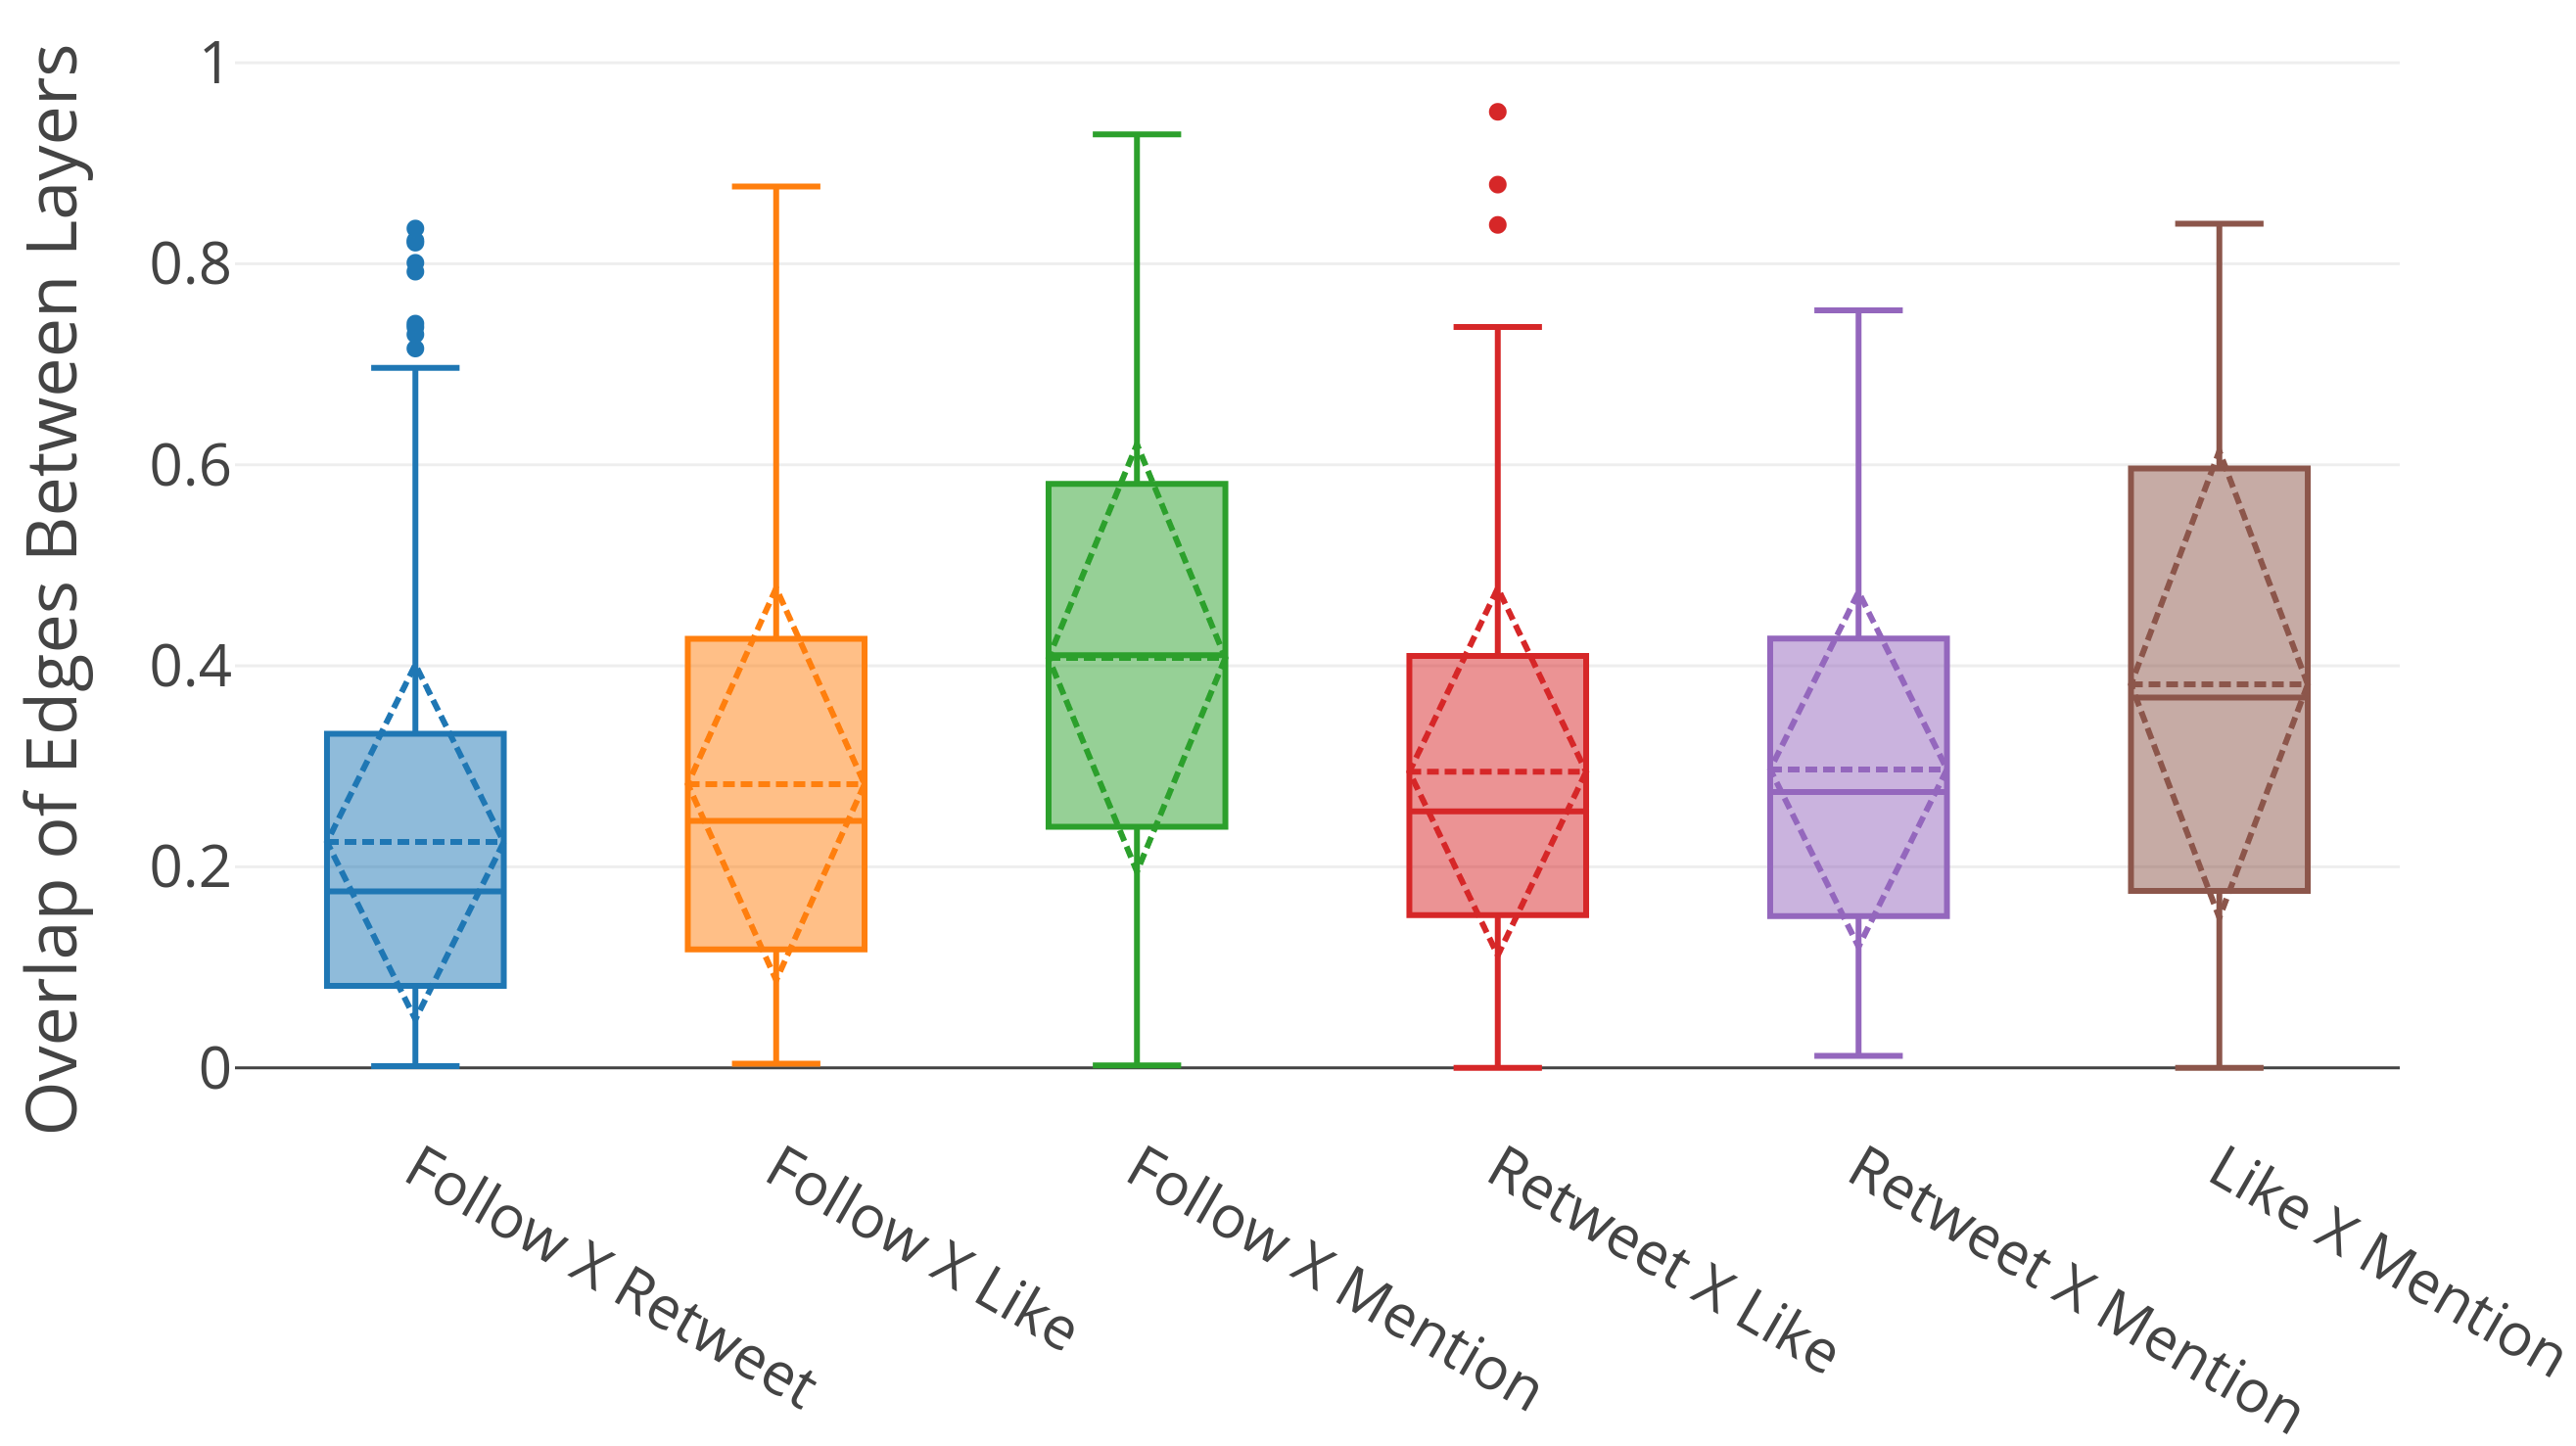
\includegraphics[width=1\textwidth]{fig/net_struct/overlap/overlap_edges_boxplot.png}
    \caption{Overlap of edges between layers.}
    \label{fig:net_struct_overlap_edges_boxplot}
\end{figure}

Edge overlap values are even smaller than vertex overlap values as shows Fig. \ref{fig:net_struct_overlap_edges_boxplot}, but, considering the small values of edge density in all layers, there still are considerable overlap, especially between the following pairs: (follow, mention) and (like, mention) with 50\% of the egos with overlay values varying between 20\% to 60\% in these layers. For the other pairs of layers, edge overlap is predominantly small, with about 75\% of the egos achieving at most 40\% of overlap values.


%%%%%%%%%%%%%%%%%%%%%%%%%%%%%%%%%%%%%%%%%%%%%% 
%%%%%%%%%%%%%%%%%%%%%%%%%%%%%%%%%%%%%%%%%%%%%% RBO
\subsection*{Rank-Biased Overlap}
\label{subsec:rbo}
Another relevant aspect of layer similarity is how many of the most important vertices in one layer are also the most important vertices in the other layer. In social networks, one common measure of importance is vertex indegree, defined in Section \ref{subsec:degree_centr}. In our context the indegree of a vertex corresponds to the number of interactions it received from the other vertices in the layer. Vertices with highest indegree values are the more preferable ones in the layer. Another vertex relevance measure commonly used is closeness centrality, defined in Section \ref{subsec:close_centr}, which measures how much a vertex is close to all the others.

\begin{figure}[ht]
    \centering
    \subfigure[Indegree ranks]{
        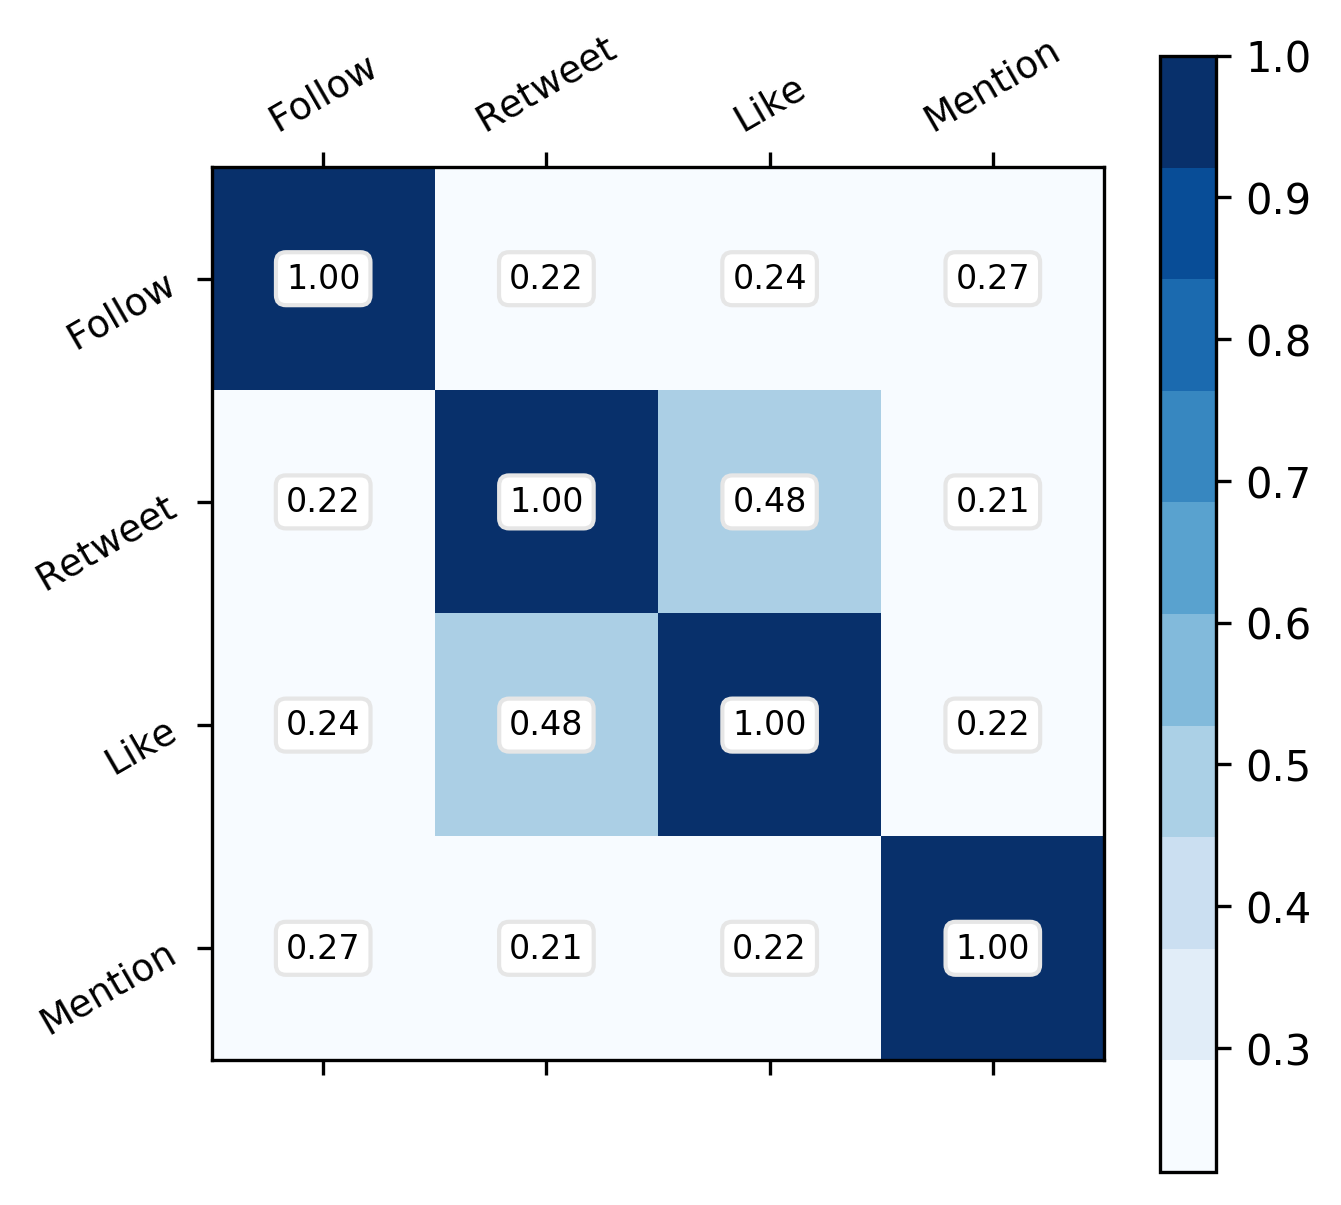
\includegraphics[width=0.45\textwidth]{fig/net_struct/rbo/rbo_in_degree_rank.png}
        \label{fig:rbo_indegree}
    }
    \subfigure[Closeness centrality ranks]{
        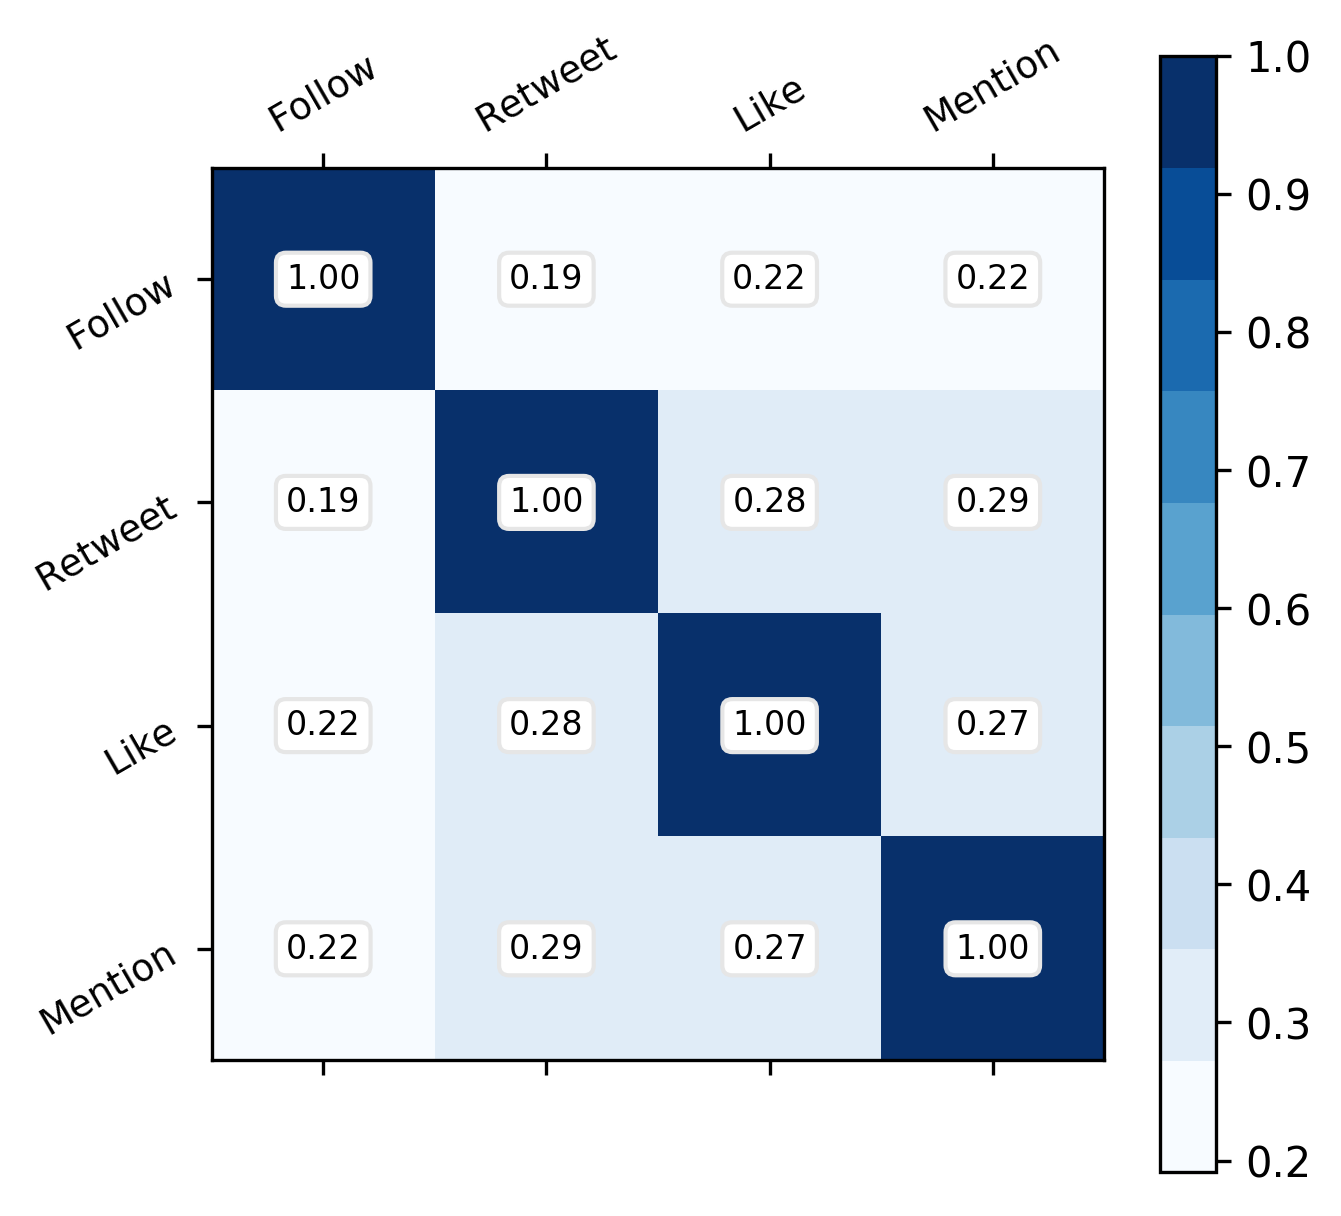
\includegraphics[width=0.45\textwidth]{fig/net_struct/rbo/rbo_close_centr.png}
        \label{fig:rbo_close_centr}
    }
    \caption{Results of extended RBO measure.}
    \label{fig:net_struct_rbo}
\end{figure}

\begin{table}[htb]
\caption{Extended RBO statistics for each pair of layers.}
\label{tab:rbo_statistics}
\centering
\scriptsize
\setlength\tabcolsep{6pt} % default value: 6pt
\begin{tabular}{|l|c|c|}
\hline 
%{{\bf Layer pair}}  &   {{\bf In-Degree Ranks}} &   {{\bf Close Centr. Ranks}} \\ \hline
\multicolumn{1}{|c|}{\textbf{Layer Pair}} & \multicolumn{1}{|c|}{\textbf{In-Degree Ranks}} & \multicolumn{1}{|c|}{\textbf{Close Centr. Ranks}} \\ \hline
\hline \hline
{Follow-Retweets}   &       0.22$\pm$0.14       &       0.19$\pm$0.10           \\ \hline
{Follow-Likes}      &       0.24$\pm$0.14       &       0.22$\pm$0.12           \\ \hline
{Follow-Mentions}   &       0.27$\pm$0.16       &       0.22$\pm$0.14           \\ \hline
{Retweets-Likes}    &       0.48$\pm$0.20       &       0.28$\pm$0.11           \\ \hline
{Retweets-Mentions} &       0.21$\pm$0.13       &       0.29$\pm$0.11           \\ \hline
{Likes-Mentions}    &       0.22$\pm$0.14       &       0.27$\pm$0.11           \\ \hline
\hline
\end{tabular}
\end{table}

We compared the rankings of vertices according to indegree and closeness centrality using the Extended RBO similarity measure discussed in Section \ref{subsec:rbo}. The mean values of Extend RBO are shown in Fig. \ref{fig:net_struct_rbo} for $p=0.98$, which implies that the top 50 vertices having about 86\% of the weight in the evaluation of the overlap between the rankings. Figure \ref{fig:rbo_indegree} shows that there is around 21\% to 27\% overlap among the 50 vertices with highest indegree values in every pair of layers, except for the pair (retweet, like), with a mean overlap of almost 50\%. The great similarity between these two rankings, may be explained by the fact that both interactions  are used to express that a tweet was considered interesting by the person who is the agent of the interactions. Because it is a mean in each pair of layers for the 500 multilayer ego networks, we enter the statistical details in the Table \ref{tab:rbo_statistics}.

The existence of intersection between the top ranked vertices in two layers is a relevant information because it shows that there are hubs (vertices with high indegree values) in at least two distinct layers. These layer-pair-wise hubs may be useful in Twitter applications related to information diffusion, since they are influential vertices in more than one type of interaction and they could, at least hypothetically, help disseminate information through the whole ego network (the composed of the union  of vertices and edges of all layers). 



%%%%%%%%%%%%%%%%%%%%%%%%%%%%%%%%%%%%%%%%%%%%%% 
%%%%%%%%%%%%%%%%%%%%%%%%%%%%%%%%%%%%%%%%%%%%%% Top-k Alters Overlap
\subsection*{Top-k Alters Overlap}
\label{subsec:topk_overlap}

We also investigated in the case of the retweet, like and mention layers if the alters with whom the ego interacts most also are her alters in the other layers. In these three layers, the ego $e$ can interact many times with a same alter $a$, by retweeting or liking many tweets authored by $a$, or by mentioning $a$ in many tweets. For the follow layer this is not the case, since the follow interaction occurs only once. To measure how many of the most interacted alters in layer $x$ were also present in other layer $z$, we first obtained the set $Top_e^x$ which is formed by the $k$ alters with whom the ego $e$ interacted most by type of interaction $x$. Next we computed fraction of elements in $Top_e^x$ that  were also in  $A_e^z$, as: $r(A_e ^z,Top_e^x) =\frac{|A_e^z \cap Top_e^x|}{k}$.

\begin{figure}[h!tb]
    \centering
    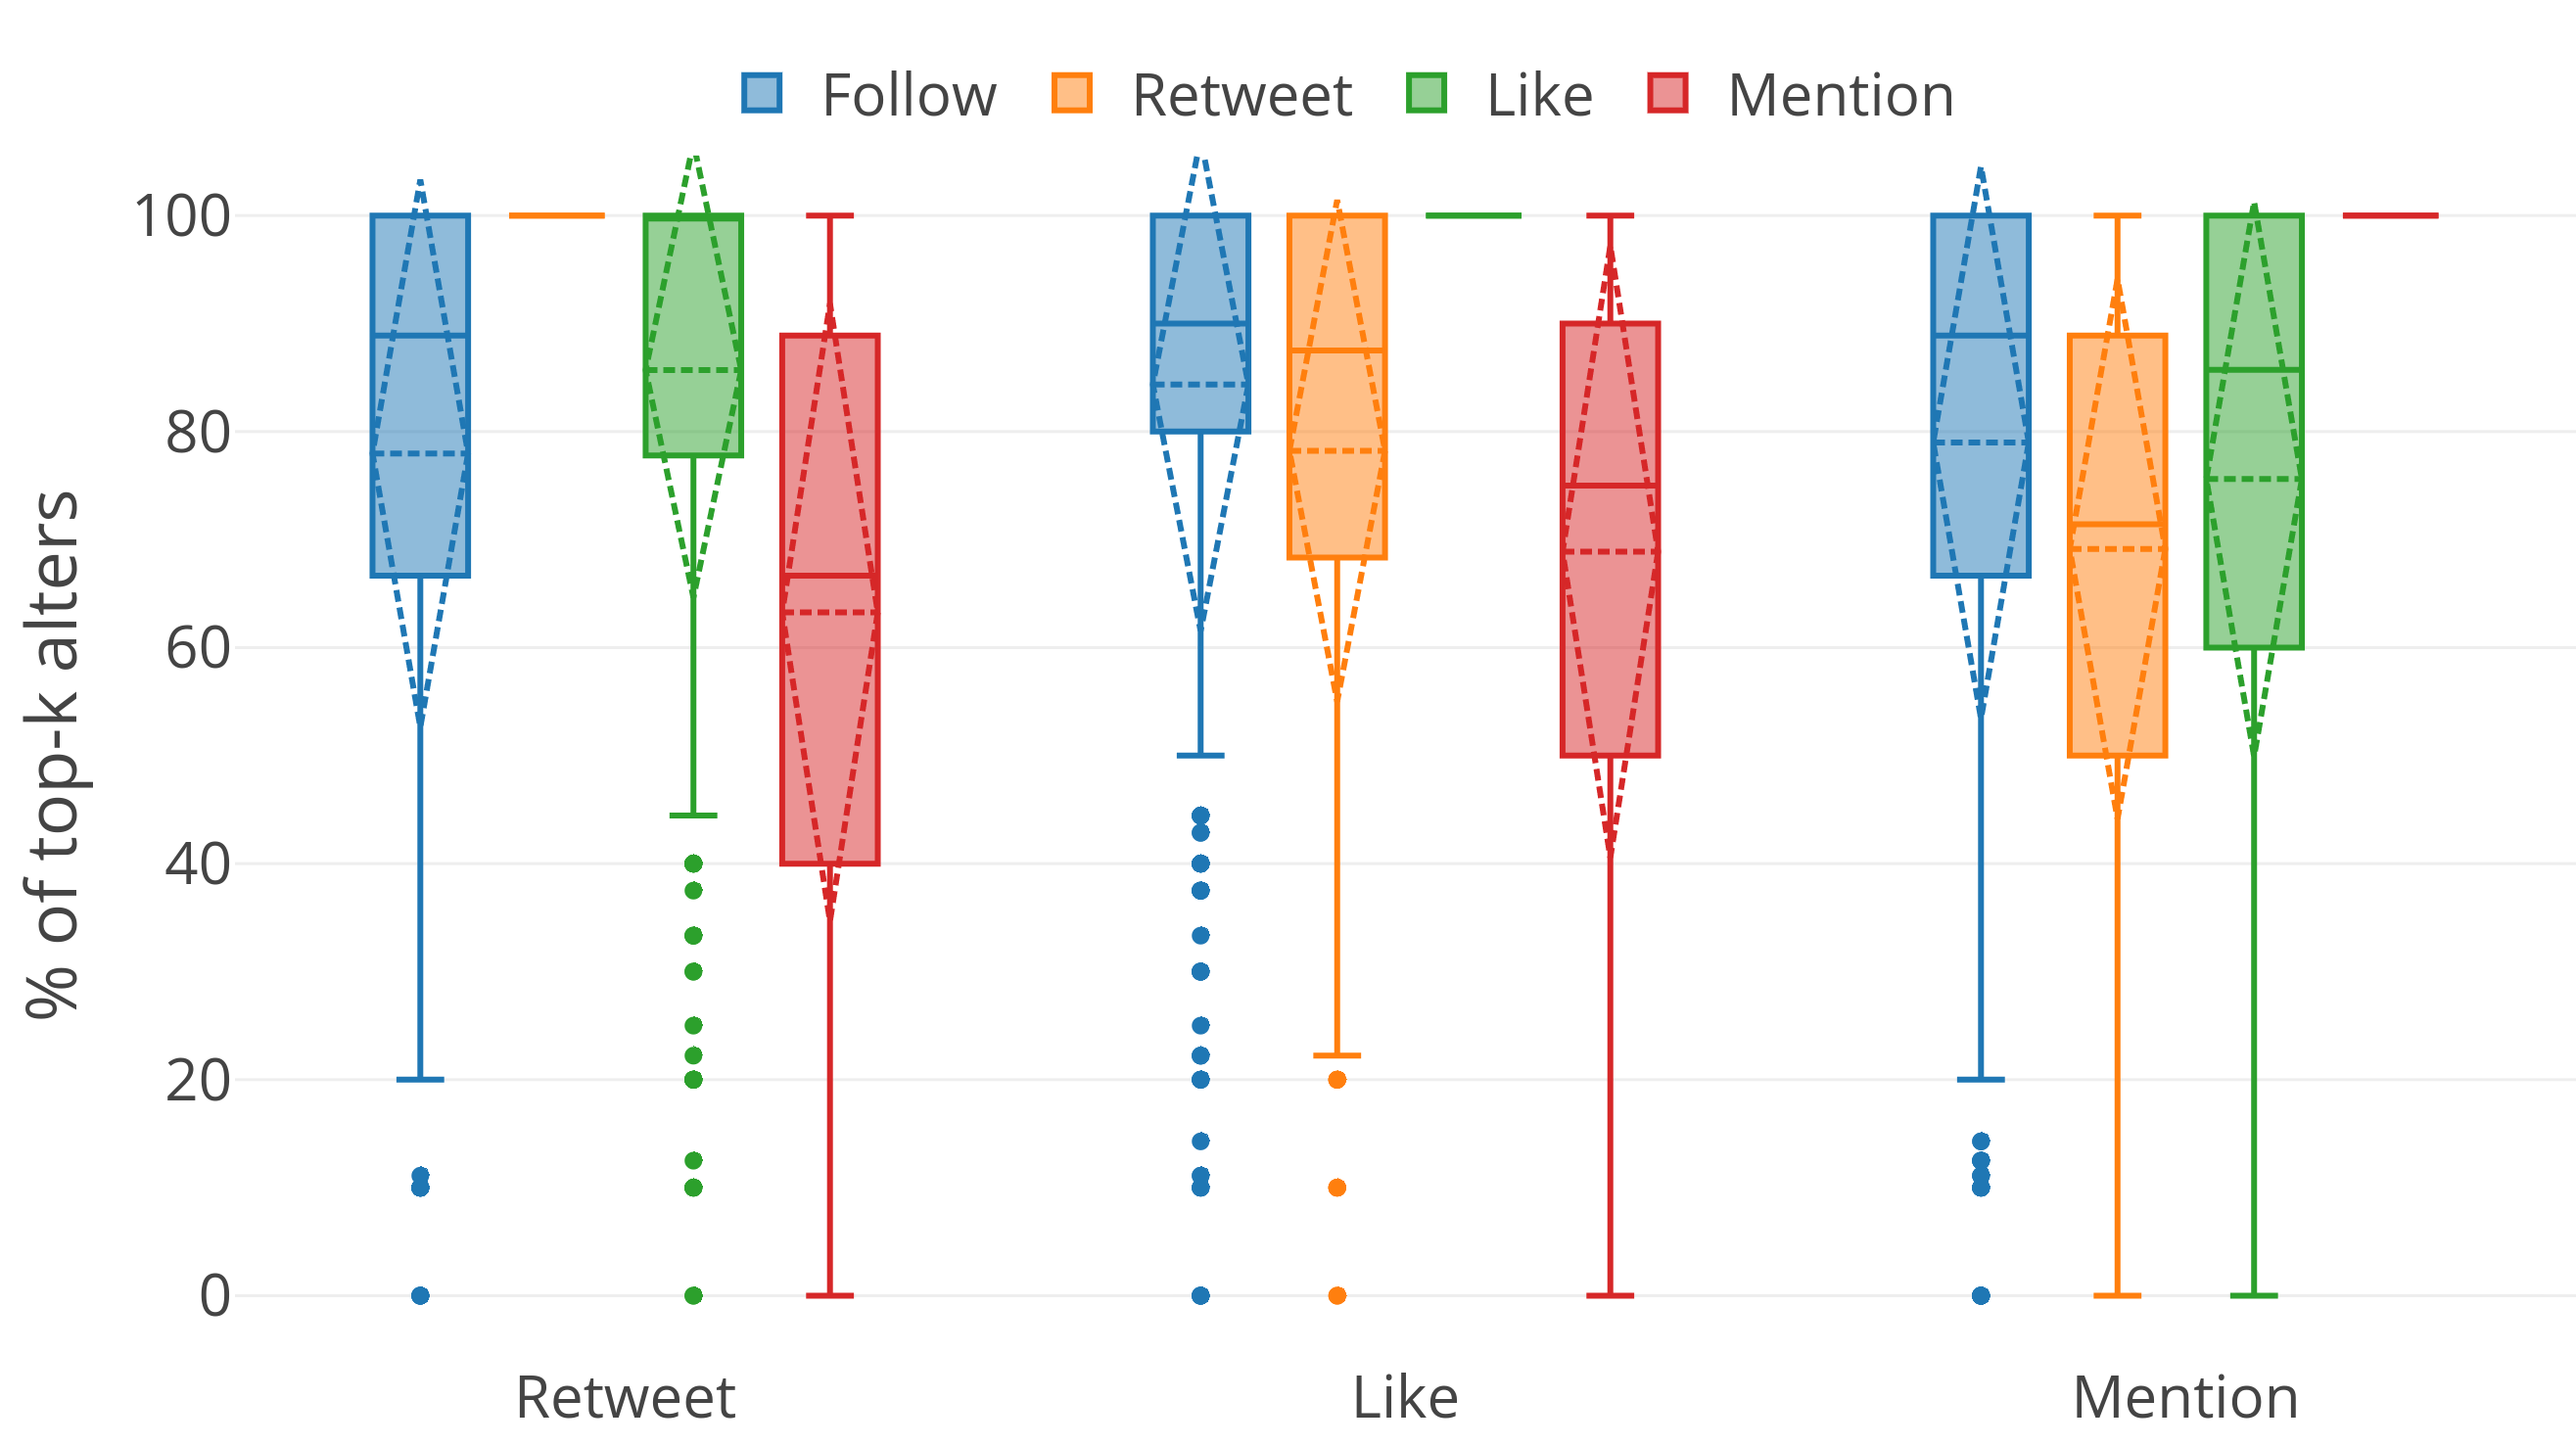
\includegraphics[width=1\textwidth]{fig/net_struct/topk_co_occurrence_boxplot.png}
    \caption{Percentage of the top-k alters of a layer that appear in the set of alters of the other layers.}
    \label{fig:net_struct_topk_over_alters}
\end{figure}

Figure \ref{fig:net_struct_topk_over_alters} shows results of this ratio for $x \in\{reteet, like, mention \}$, for $k=10$. For each layer (x axis), Fig. \ref{fig:net_struct_topk_over_alters} shows four box plots representing the distribution of $r(A_e ^z,Top_e^x)$, for $z \in\{follow,like, retweet, mention\}$. The results shows that there is also a great variability on the values of $r(A_e ^z,Top_e^x)$, with some egos having no alter in $Top_e^x$ occurring in another alter set $A_e^x$ and some egos where the all elements in $Top_e^x$ occurring in another alter set. For most egos the ratio values are high, but it is clear from the figure that the top 10 alters most interacted with by the retweet and like interaction are the ones that occur less in the mention layer, contributing to reinforce lack of affinity between the like and mention interaction and also between the retweet and mention interactions. Besides, we can observe more affinity between the retweet and like layers with most egos having the top 10 alters in one of these layers also being alters in the other layer. 

We find that the for all the tree layers (retweet, like and mention) the top 10 alters in these layers tend to occur frequently in the follow layer. But, it is important to remember that this fact may be due to limitations on the construction of the alter sets reported in Section \ref{cap:ExpSetup}, with the alter set for the follow layer being bigger than the alter set of the remaining layers for most egos. Despite the high values of the ratio regarding the follow layer, the blue box plots in Figure \ref{fig:net_struct_topk_over_alters} reveal an interesting problem: {\em many users may not receive all the tweets produced by the alters they interact most with retweets, likes and mentions}. As the box plots show, for about 25\% of the egos, their most retweeted alters are not followed by them, and 50\% of egos do not follow 20\% of their most retweeted alters (left most blue box plot in the figure). A similar situation can be seen with the most mentioned alters (rightmost blue box plot).

The miss of tweets coming from this most preferable alters may occur because the egos do not follow these alters. When a user $e$ follows another user $a$ in Twitter, all the tweets authored or retweeted by $a$ are propagated to $e$’s  timeline. If $e$ does not follow $a$, $e$ receives a tweet retweeted or authored by $a$ only if another user followed by $e$ retweets this tweet. This implies that if a tweet produced or retweet by $a$ may not reach $e$’s timeline if none of the followees of $e$ retweet it. In this case, $e$ may be missing information produced by her most preferable tweet producers. 

When considering the retweet interaction, the above problem may have another implication: if a tweet authored by a preferable alter regarding the retweet interaction is not delivered in the ego’s timeline the tweet loses a great chance to be propagated in the network by an ego with a great probability of retweeting it, affecting information cascading in Twitter. The above problem may be diminished by recommending to a user to follow people to whom they interact most by retweets, likes and mention and who she is not following yet. Twitter has a user recommendation service, but it not known if the service suggests the type of recommendation just mentioned above.



%%%%%%%%%%%%%%%%%%%%%%%%%%%%%%%%%%%%%%%%%%%%%% 
%%%%%%%%%%%%%%%%%%%%%%%%%%%%%%%%%%%%%%%%%%%%%% 



\section{Do the indegree distributions follow a power-law?}
\label{sec:QuestionPowerLaw}

\begin{figure}[h!tb]
    \centering
    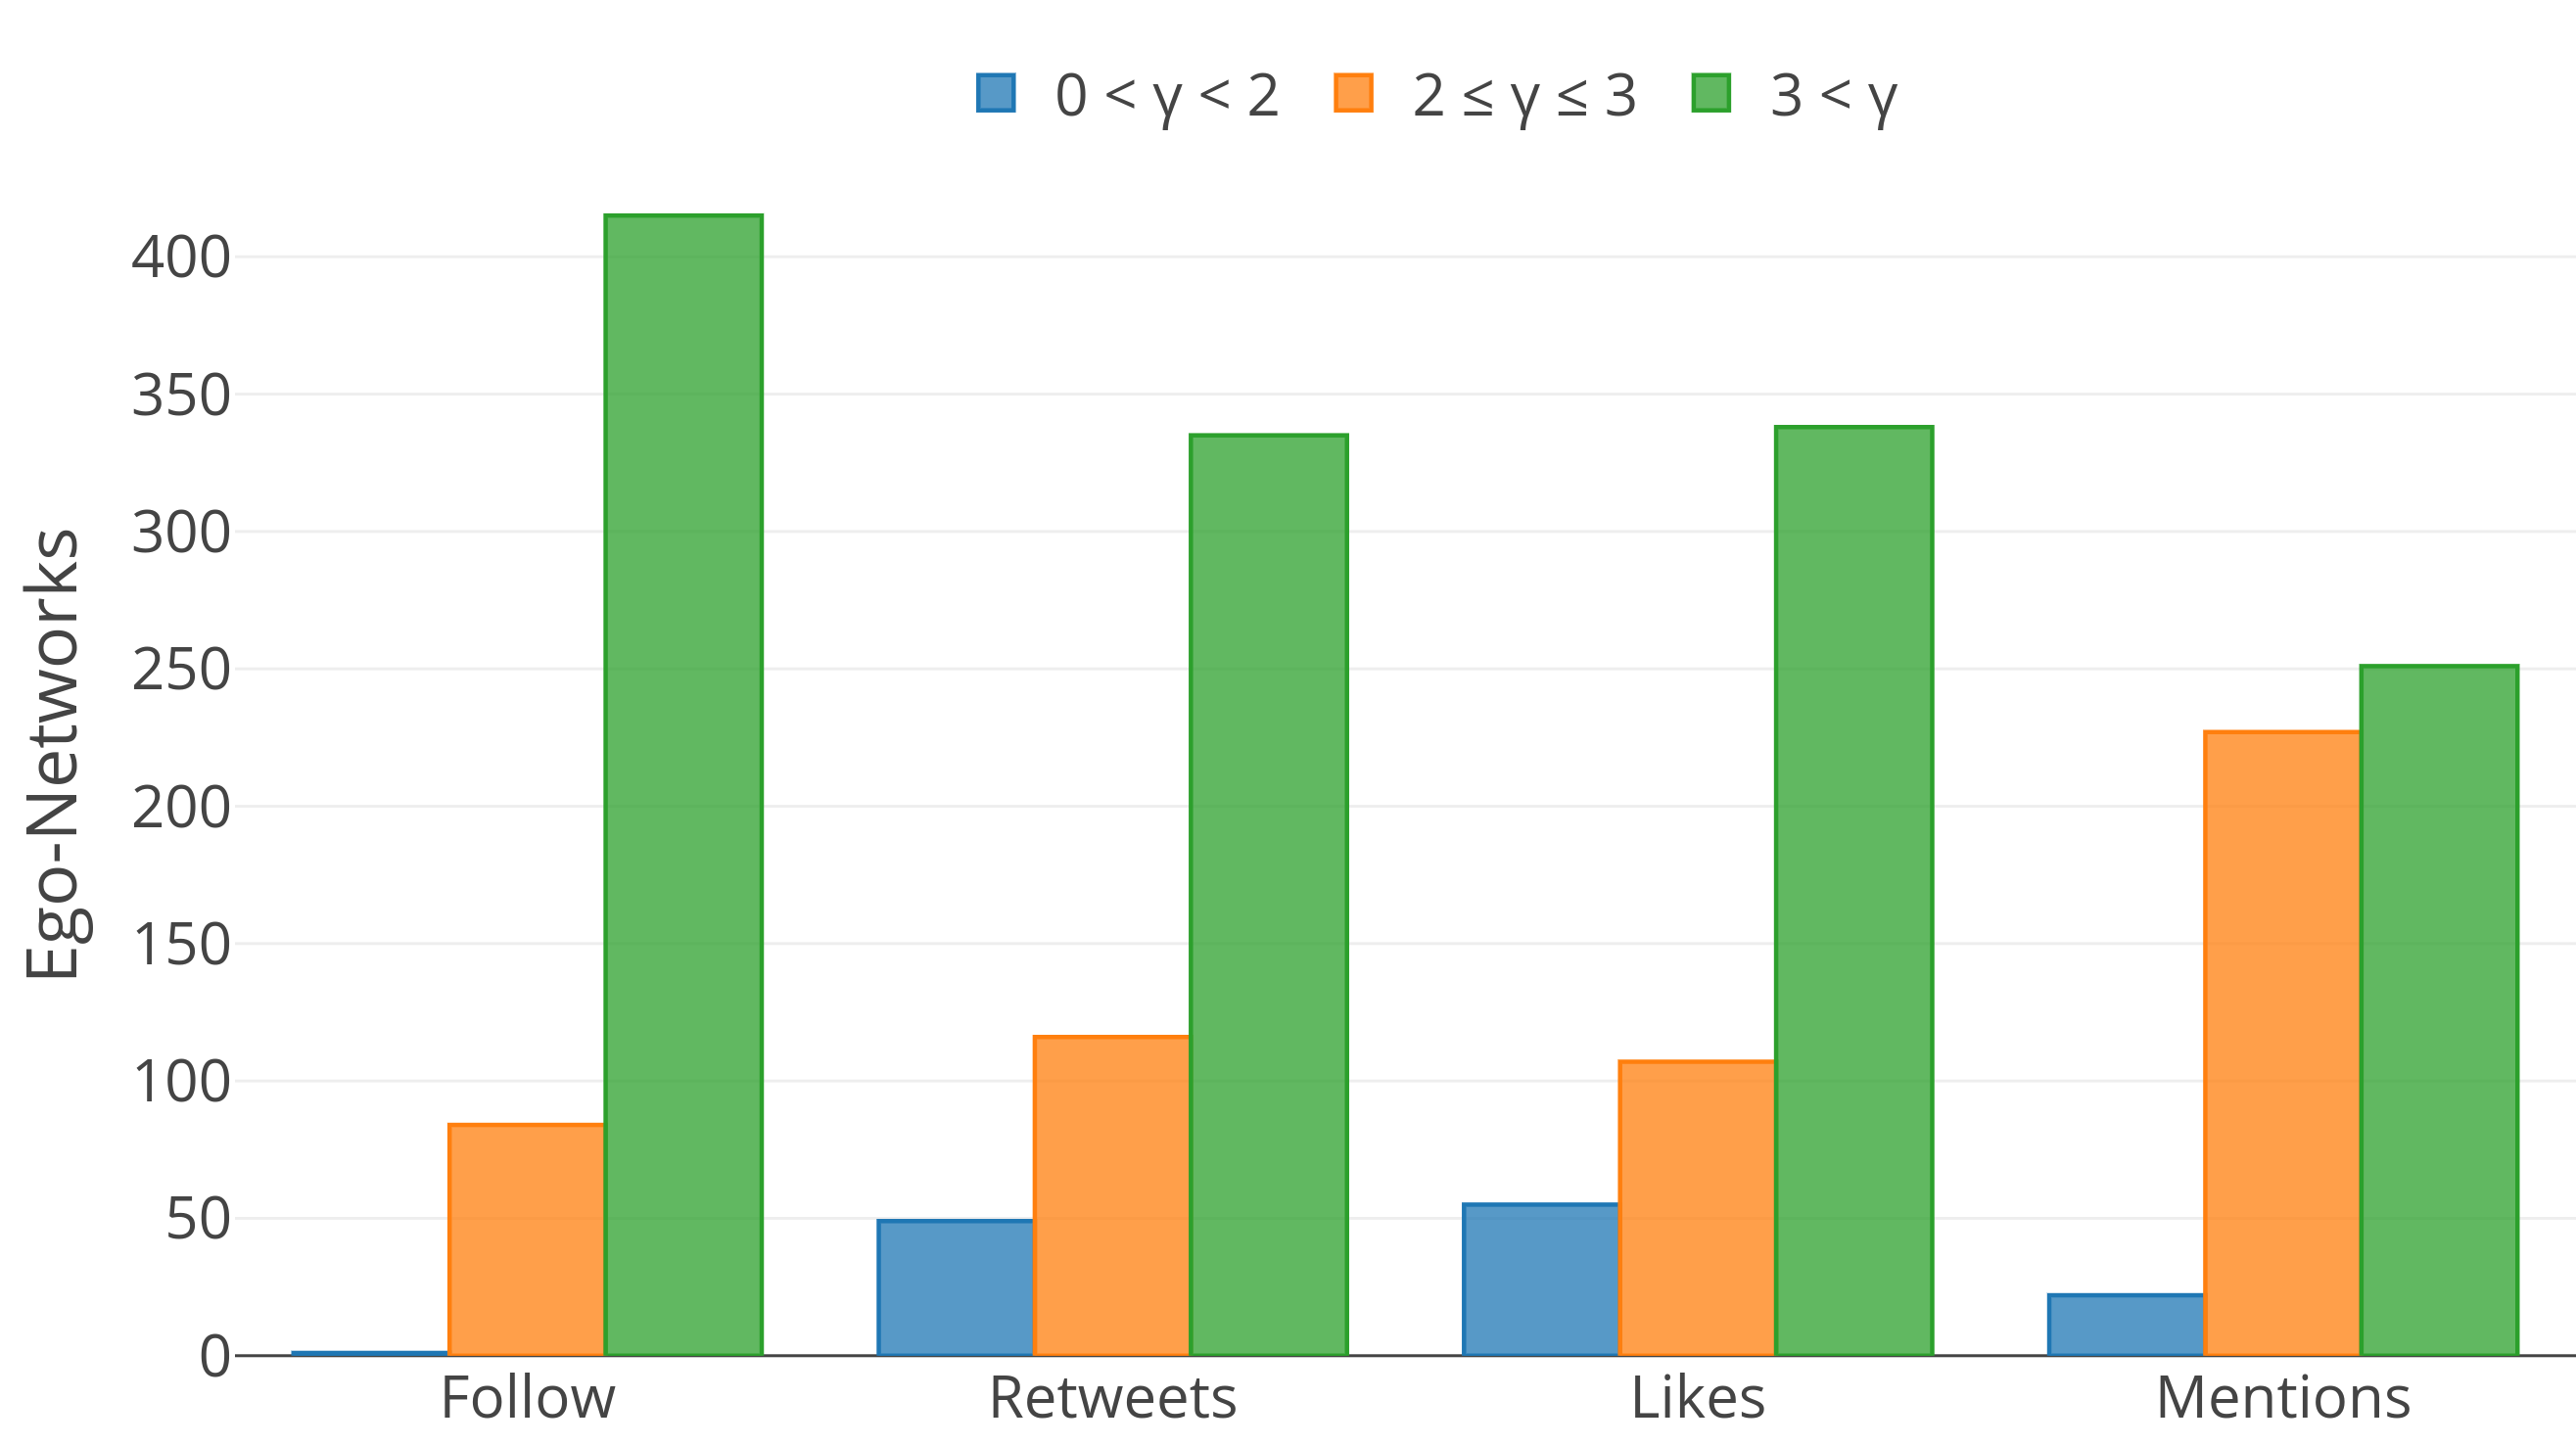
\includegraphics[width=1\textwidth]{fig/net_struct/in_degree_distribution.png}
    \caption{Classification of the ego networks as to the distribution of the indegree.}
    \label{fig:net_struct_indegree_distribution}
\end{figure}

We verifyied if the the indegree distributions in all layers followed a power-law, i.e., if they could be described by Eq. \ref{eq:1}. We used the Powerlaw Python package \cite{Alstott2014} to find the appropriate functions to fit the data. We found that indegree distributions in all layers follow a power-law, but as happens with all the other aspects analyzed, there is great variation on the results. Diverse variations of $\gamma$ values we found. We classified the distributions in three categories: Category A with $0<\gamma <2$; Category B, with $2<\gamma<3$ and Category C, with $\gamma> 3$. This categorization was used because most networks found in nature and those derived from human activities are known to follow a power-law with $2<\gamma<3$, i.e., belong to Category B. Thus, we adopted the interval corresponding to Category B to separate layers  that fit a “standard power-law” (Category B) from those that are apart from the standard, with inferior $\gamma$ values (Category A) or superior $\gamma$ values (Category C).

Figure \ref{fig:net_struct_indegree_distribution} shows the distribution of categories found in each layer. Despite the existence of very different $\gamma$ values, for most egos, the indegree distribution in the follow, retweet and like layers follow a power-law distribution of Category C. The mention layer is the one that most approaches what we refer to “standard power-law” regarding  the indegree distributions, since the number of egos whose mention layers fallow in Category B is the largest, comparing to the other layers. The consequence of these observations is that for the great majority of egos we have in all layers  very few alters who are the target of many interactions originated from the other alters or form the ego. On the other hand, the great majority of alters (the long tail) receive very few interactions in the layers. 



%%%%%%%%%%%%%%%%%%%%%%%%%%%%%%%%%%%%%%%%%%%%%% 
%%%%%%%%%%%%%%%%%%%%%%%%%%%%%%%%%%%%%%%%%%%%%% 



\section{Are the layers small-world graphs?}
\label{sec:QuestionSmallWorld}

We analyze whether each layer of multilayer ego networks can be classified as small-worlds. For this we use the definition presented in section \ref{sec:small_worlds}, which uses a trade-off between clustering coefficient and average shortest path length (ASPL), comparing them with an equivalent random graph, with the same number of vertices and edges. The clustering coefficient was calculated using the formula described in Eq. \ref{eq:locClustCoef}, and the ASPL was calculated as described in \cite{Mao2013}, which uses the ratio of the sum of all minimum paths between all vertices about the number of existing shortest paths, according to Eq. \ref{eq:ASPL}.

\begin{figure}[h!tb]
    \centering
    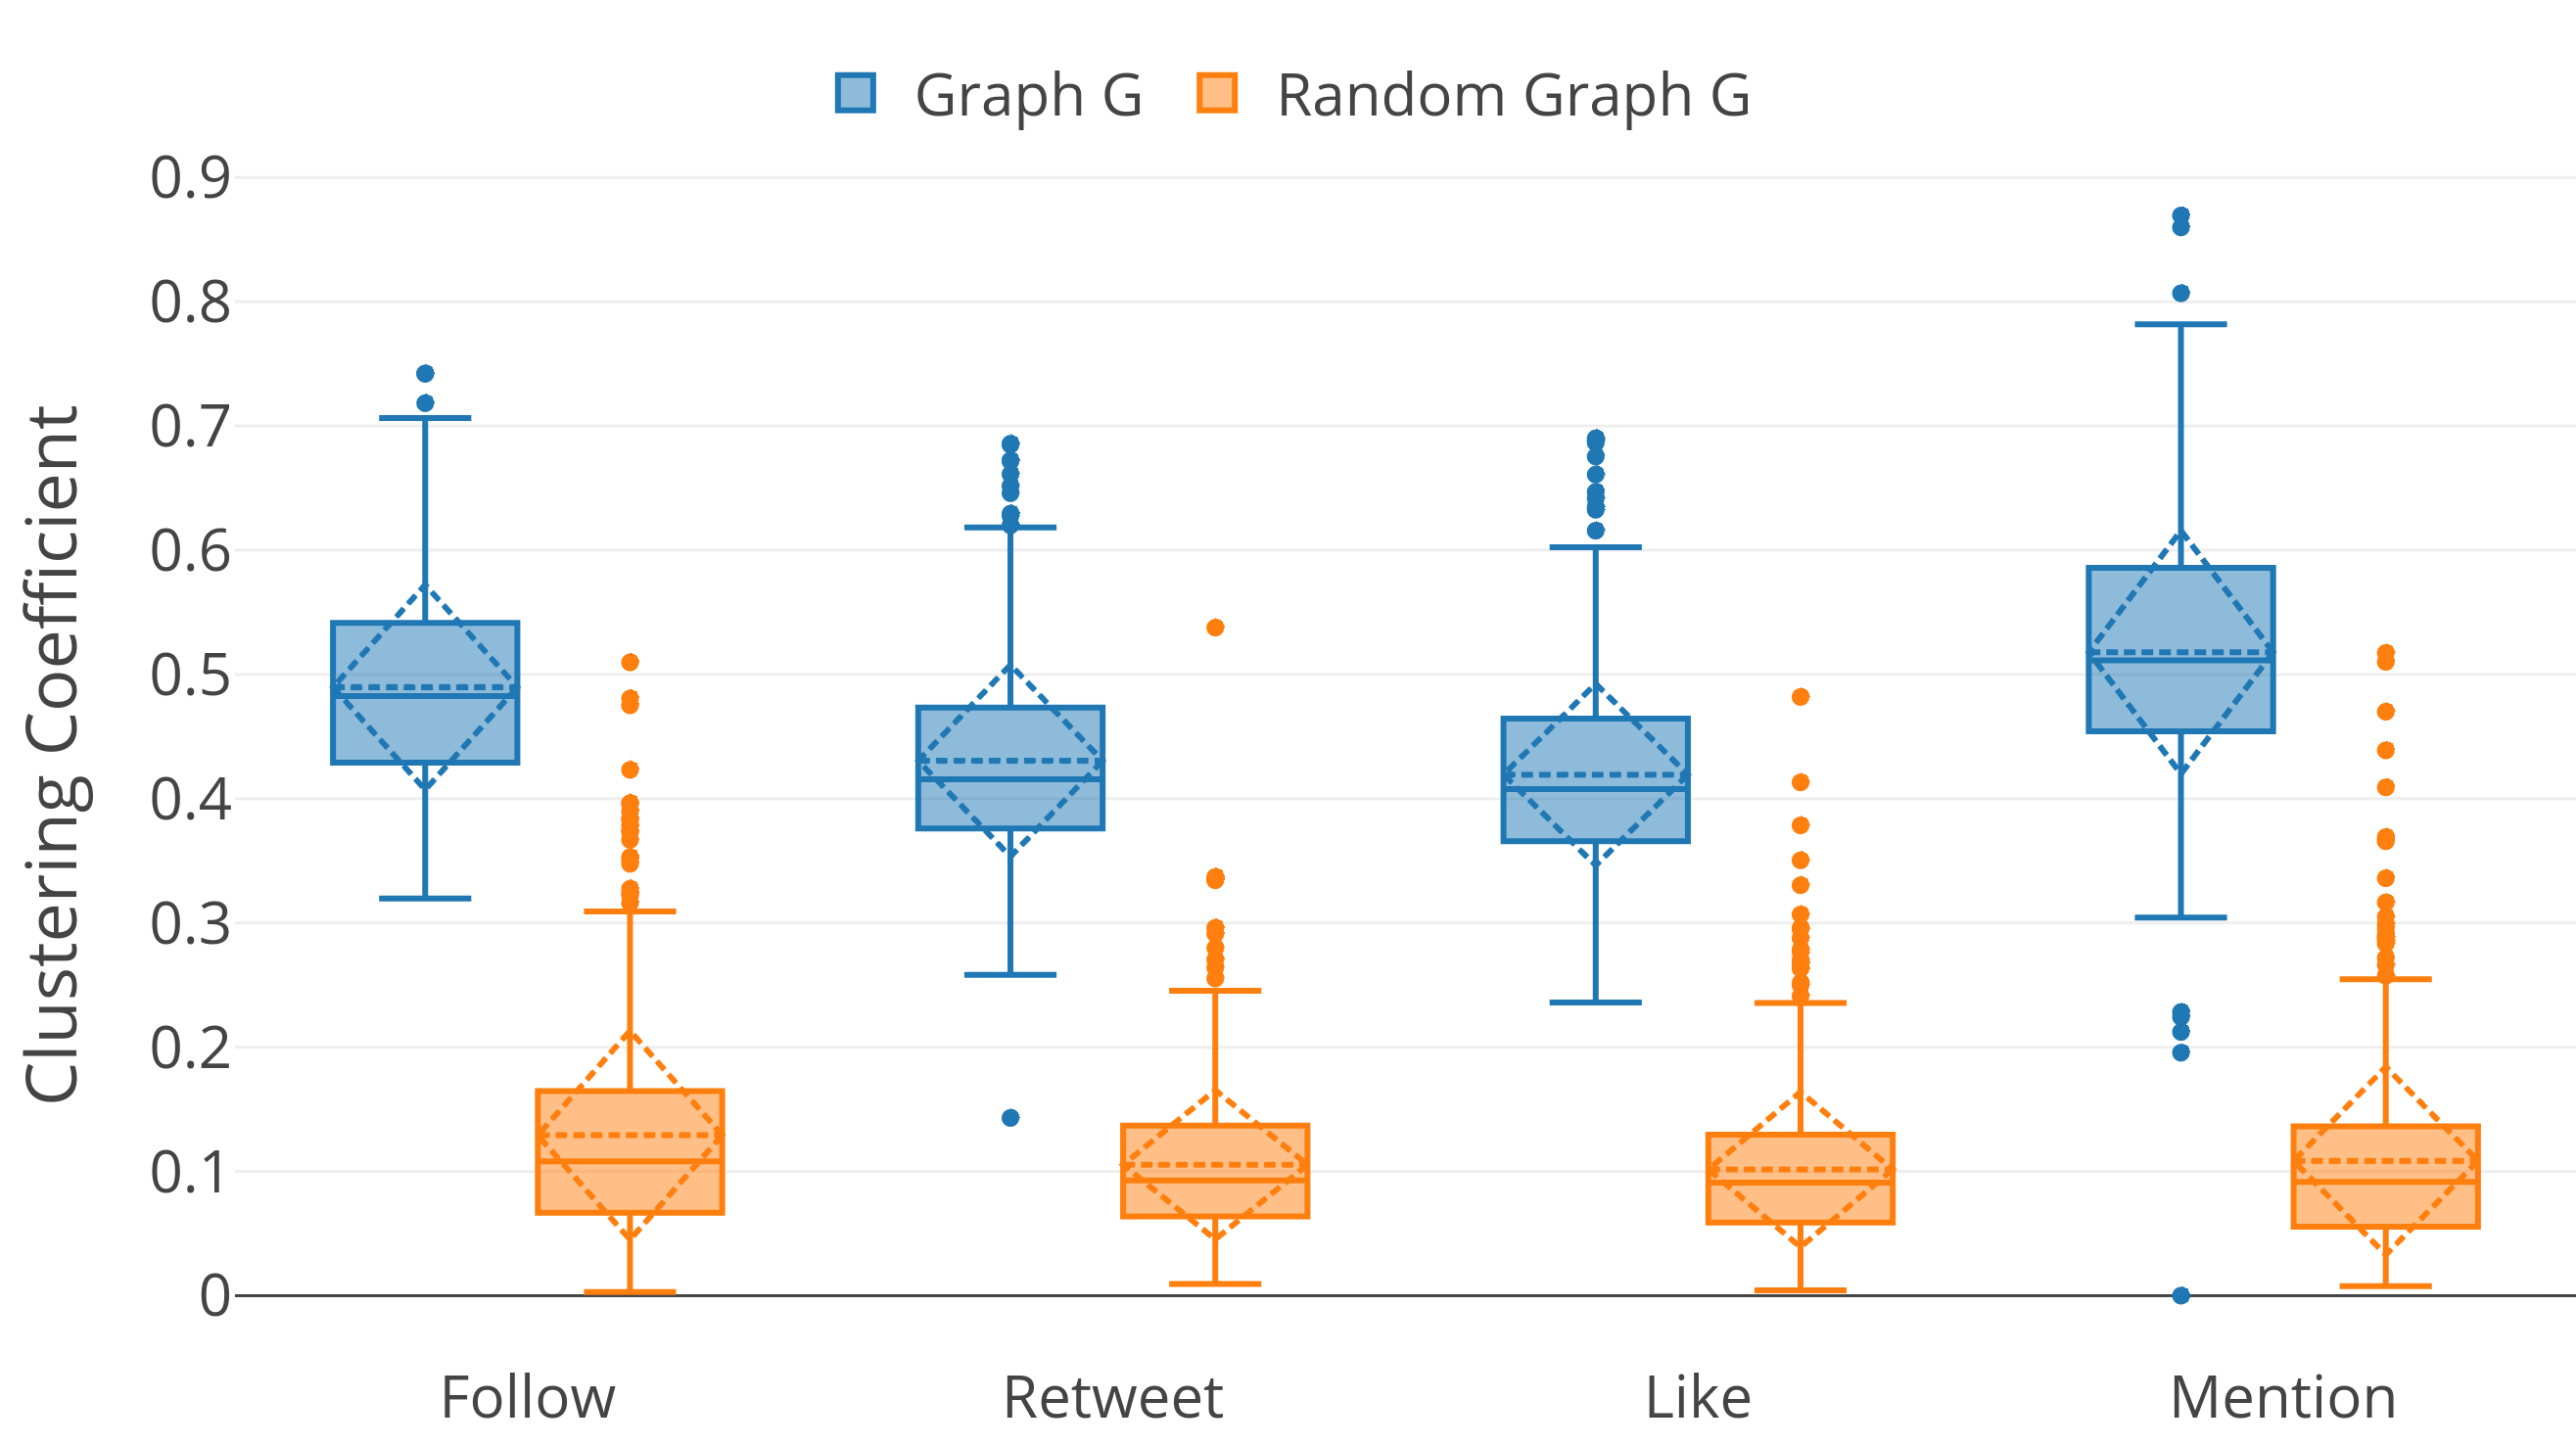
\includegraphics[width=1\textwidth]{fig/net_struct/coef_clust_rnd_g.png}
    \caption{Clustering coefficient of graph G and random graph G.}
    \label{fig:net_struct_coef_clust_rnd_g}
\end{figure}

\begin{figure}[h!tb]
    \centering
    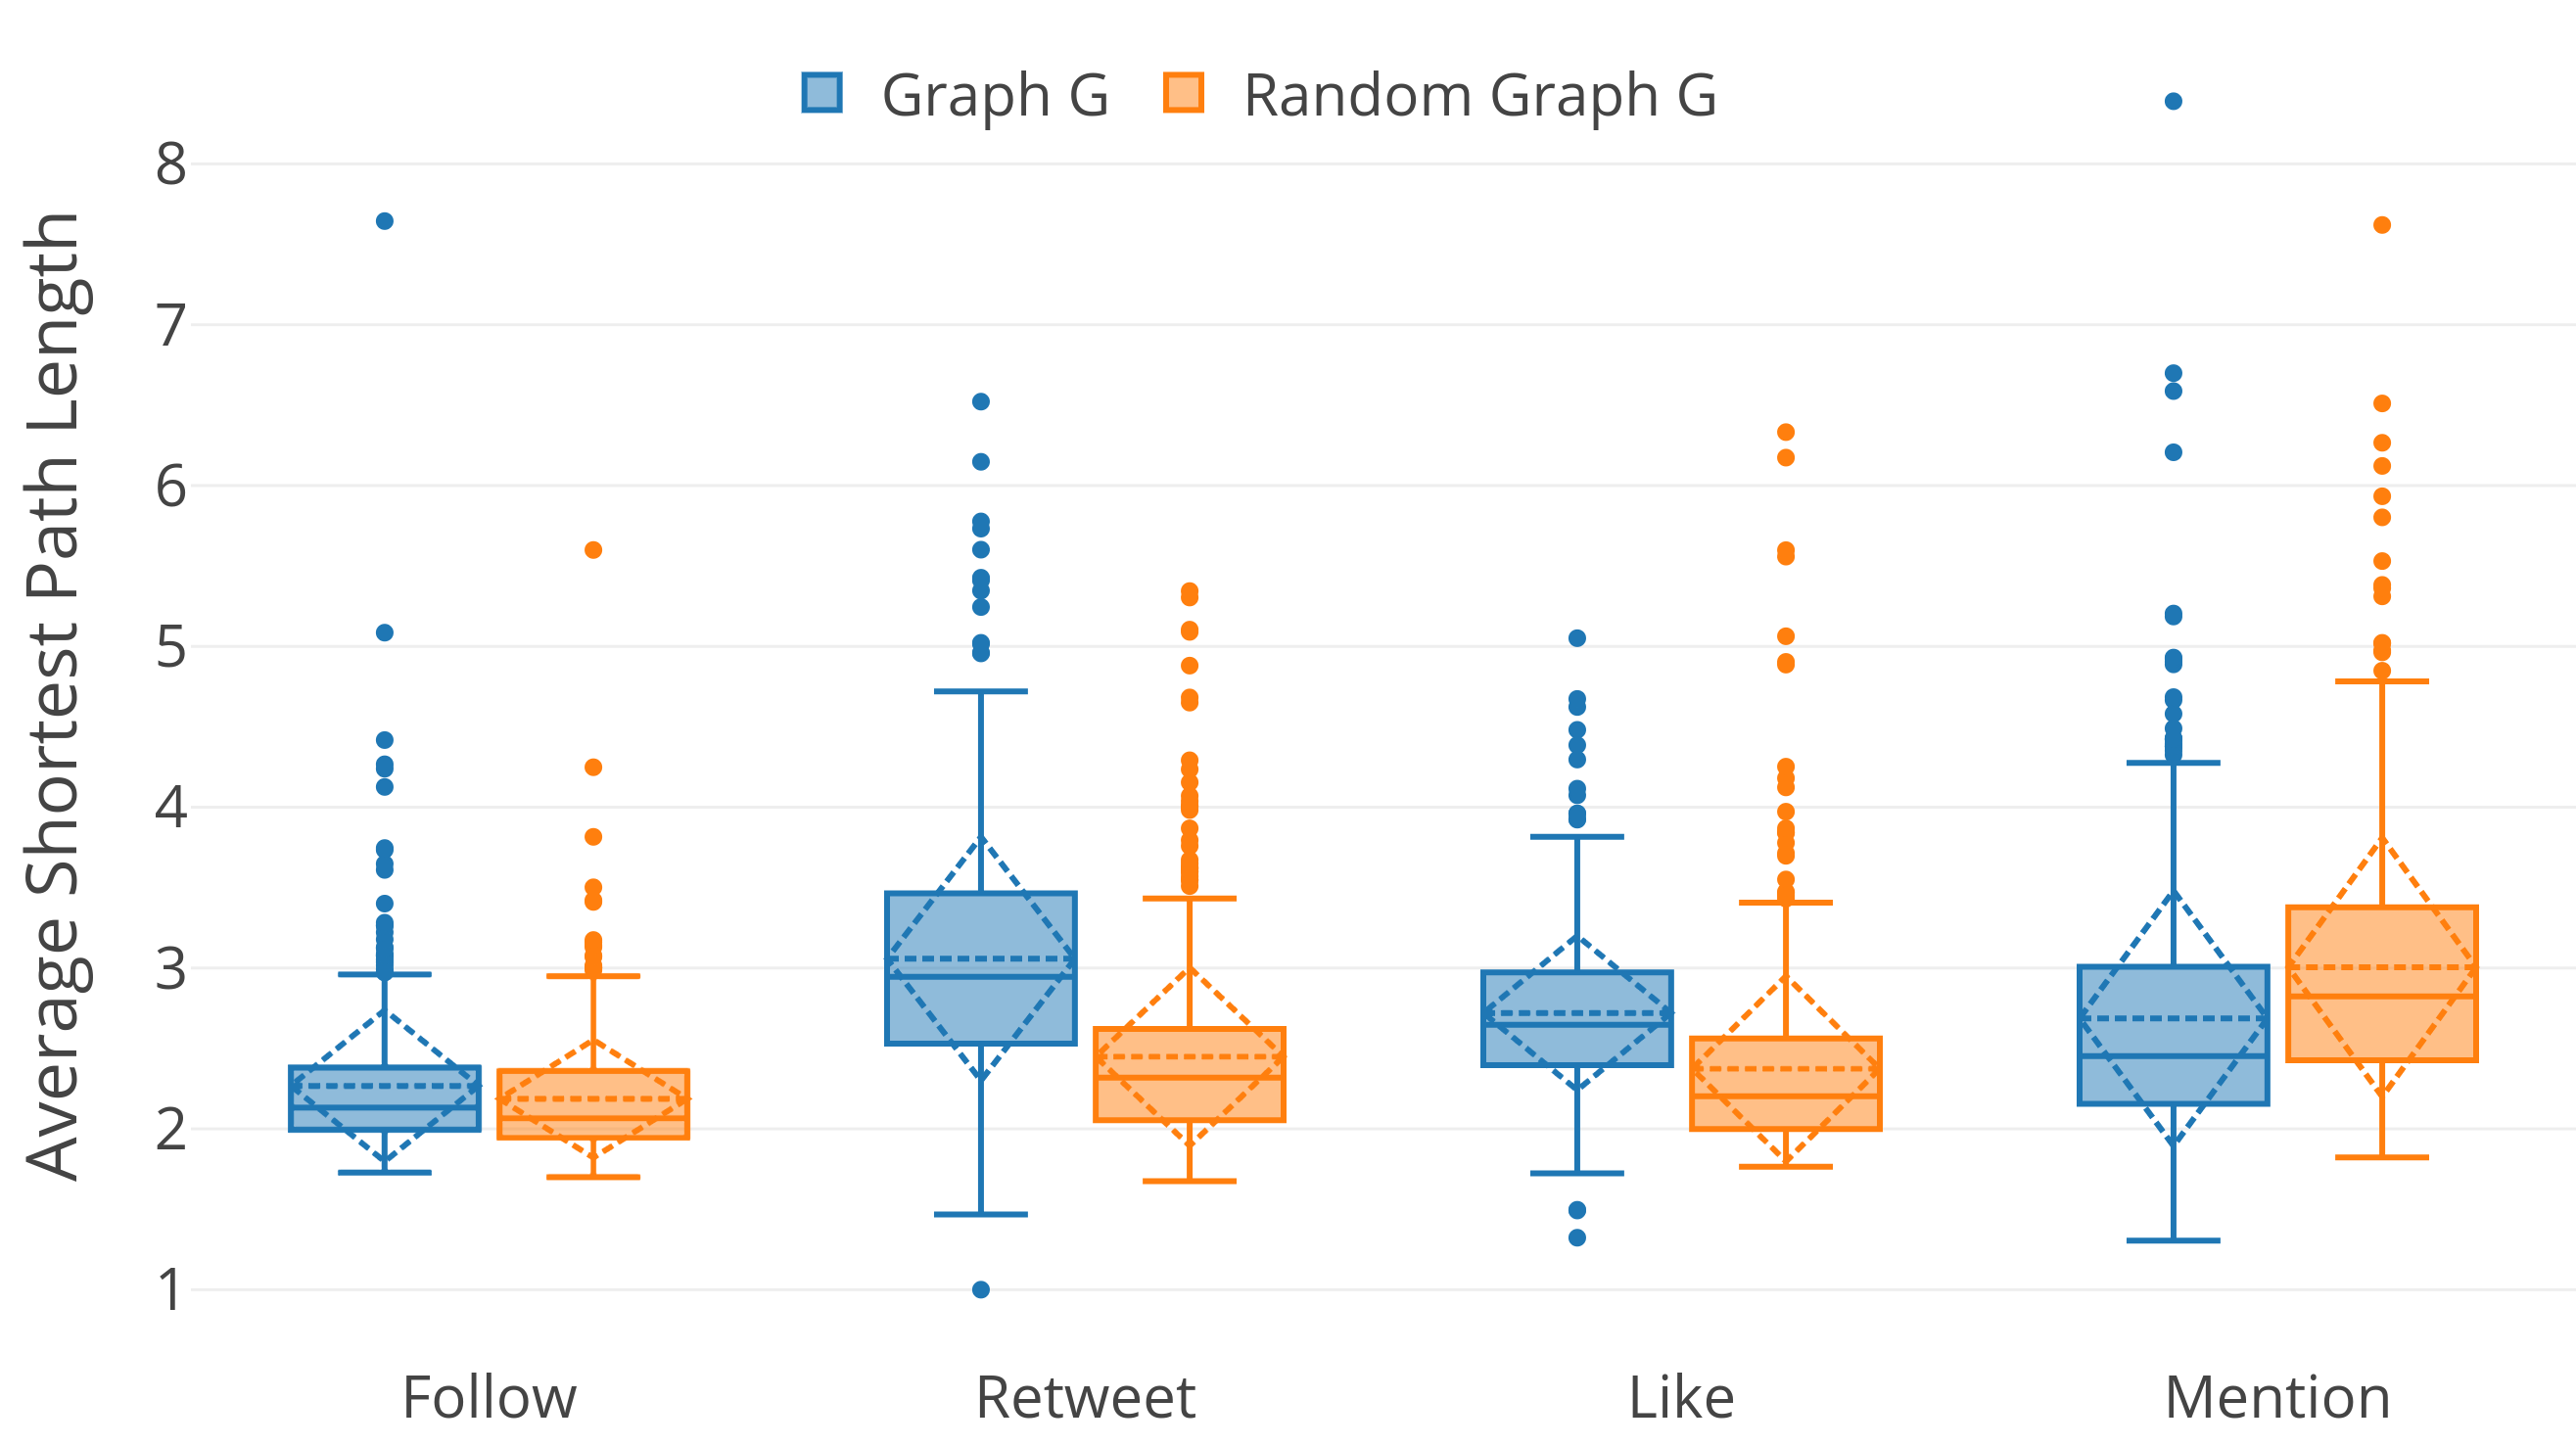
\includegraphics[width=1\textwidth]{fig/net_struct/aspl_rnd_g.png}
    \caption{Average shortest path length of graph G and random graph G.}
    \label{fig:net_struct_aspl_rnd_g}
\end{figure}


The Fig. \ref{fig:net_struct_coef_clust_rnd_g} presents the results of the average of the local clustering coefficient of each graph in each layer, and an equivalent Erd\"{o}s-R\'{e}nyi (E$-$R) random graph $G_{E-R}$. The results clearly show that all the layers have high coefficients of grouping of the graphs with respect to the equivalent random graph, indicating that the vertices tend to group with their neighbors, forming communities. The  Fig. \ref{fig:net_struct_aspl_rnd_g} presents the results of the calculation of ASPL for each graph and an equivalent Erd\"{o}s-R\'{e}nyi (E$-$R) random graph $G_{E-R}$, in each layer analyzed. The results show that all layers have low ASPL values, with almost all analyzed graphs showing values between 1.5 and 5. For the Retweet and Like layers the ASPL values are on average larger than the random graph; for the Follow layer the ASPL values are very similar to those found in the random graphs, and only the Mentions layer has on average lower ASPL values than the random graph.

With the values found we could classify the ego networks in small worlds using the metric $S$, according to Eq. \ref{eq:S}.The results were arranged in the table \ref{tab:small_world}. We can observe that all 500 graphs of the Follow, Retweet and Like layers obtained values of $S$ greater than 1, and only two graphs in the Mention layer obtained results equal to or lower than 1 for the metric $S$, possibly outliers, as can be observed in the figures \ref{fig:net_struct_coef_clust_rnd_g} and \ref{fig:net_struct_aspl_rnd_g}. These results show that practically all layers have graphs that can be classified as small-worlds.

\begin{table}[h!tb]
    \renewcommand{\arraystretch}{1.3}
    \caption{Number of ego-networks classified in small world according to metric S}
    \label{tab:small_world}
    \centering
    \scriptsize
    \setlength\tabcolsep{6pt} % default value: 6pt
    \begin{tabular}{|c|c|c|}
        \hline
        {\bf Layer} &   {\bf$S \leq 1$} &   {\bf$1 < S$ }\\ \hline \hline
        Follow      &       -       &       500     \\  \hline
        Retweet     &       -       &       500     \\  \hline
        Like        &       -       &       500     \\  \hline
        Mention     &       2       &       498     \\  \hline\hline 
    \end{tabular}
\end{table}

%%%%%%%%%%%%%%%%%%%%%%%%%%%%%%%%%%%%%%%%%%%%%% 
%%%%%%%%%%%%%%%%%%%%%%%%%%%%%%%%%%%%%%%%%%%%%% 


\section{How is each layer structured in communities?}
\label{sec:QuestionCommunities}

%\section{Configuring Community Detection Algorithms}
%\label{sec:exp_alg_comm_detection}
To investigate if layers are organized in communities we applied different community detection algorithms in all layers of all ego networks considered. The algorithms used are described in the Table \ref{tab:CommDetectionAlgs}. These algorithms are widely used in the work of community detection in graphs, so they are already consolidated algorithms, and were selected according to criteria related to computational complexity, application in directed networks, detection capacity of disjoint or overlapping communities - taking into account the realities of OSNs - and availability of software access. Its characteristics have been described in the section \ref{sec:comm_algorithms}.

The COPRA algorithm required a specific parameter ($v$), which determines the maximum number of communities that a vertex can be associated with. As pointed out by Wu et al. \cite{Wu2012}, the choice of parameter $v$ is difficult and induces the non-determinism of COPRA, since, because it is global vertex-independent parameter, it does not take into account that a large number of vertices do not overlap while few vertices participate in many communities. In our experiment we used $v = 2$.  Because COPRA is an extension of the RAK algorithm, running COPRA with $v=1$ causes the RAK algorithm itself to run. Therefore, we use the same code to achieve COPRA and RAK results. For the other algorithms the standard configuration of each was used. 

\begin{table}[h!tb]
   \renewcommand{\arraystretch}{1.3}
    \caption{Algorithms for detecting communities used in experiments.}
    \label{tab:CommDetectionAlgs}
    \centering
    \scriptsize
    \setlength\tabcolsep{6pt} % default value: 6pt
    \begin{tabular}{|c|c|c|c|}
        \hline
		\textbf{Algorithm}              &   \textbf{Type of Community}  & \textbf{Version}  & \textbf{Available in} \\ \hline
		RAK \cite{Raghavan2007}      	&   Disjoint                    & 1.24              & http://gregory.org/research/networks/software \\ \hline
			
		INFOMAP \cite{Rosvall2008}&   Disjoint                    & 0.19.x            & http://www.mapequation.org/code.html \\ \hline
					
		COPRA \cite{Gregory2010}      	&   Overlapping                 & 1.24              & http://gregory.org/research/networks/software \\ \hline
			
		OSLOM \cite{Lancichinetti2011} 	&   Overlapping                 & 2.4               & http://www.oslom.org \\ \hline
			
    \end{tabular}
\end{table}

%To investigate if layers are organized in communities we applied different community detection algorithms in all layers of all ego networks considered. The algorithms used were COPRA \cite{Gregory2010} and OSLOM \cite{Lancichinetti2011} for overlapping communities detecion; and RAK \cite{Raghavan2007} and INFOMAP \cite{Rosvall2008} for disjoint community detection. 


%Número de comunidades detectadas por cada algoritmo
\begin{figure}[h!tb]
    \centering
    \subfigure[Follow]{
        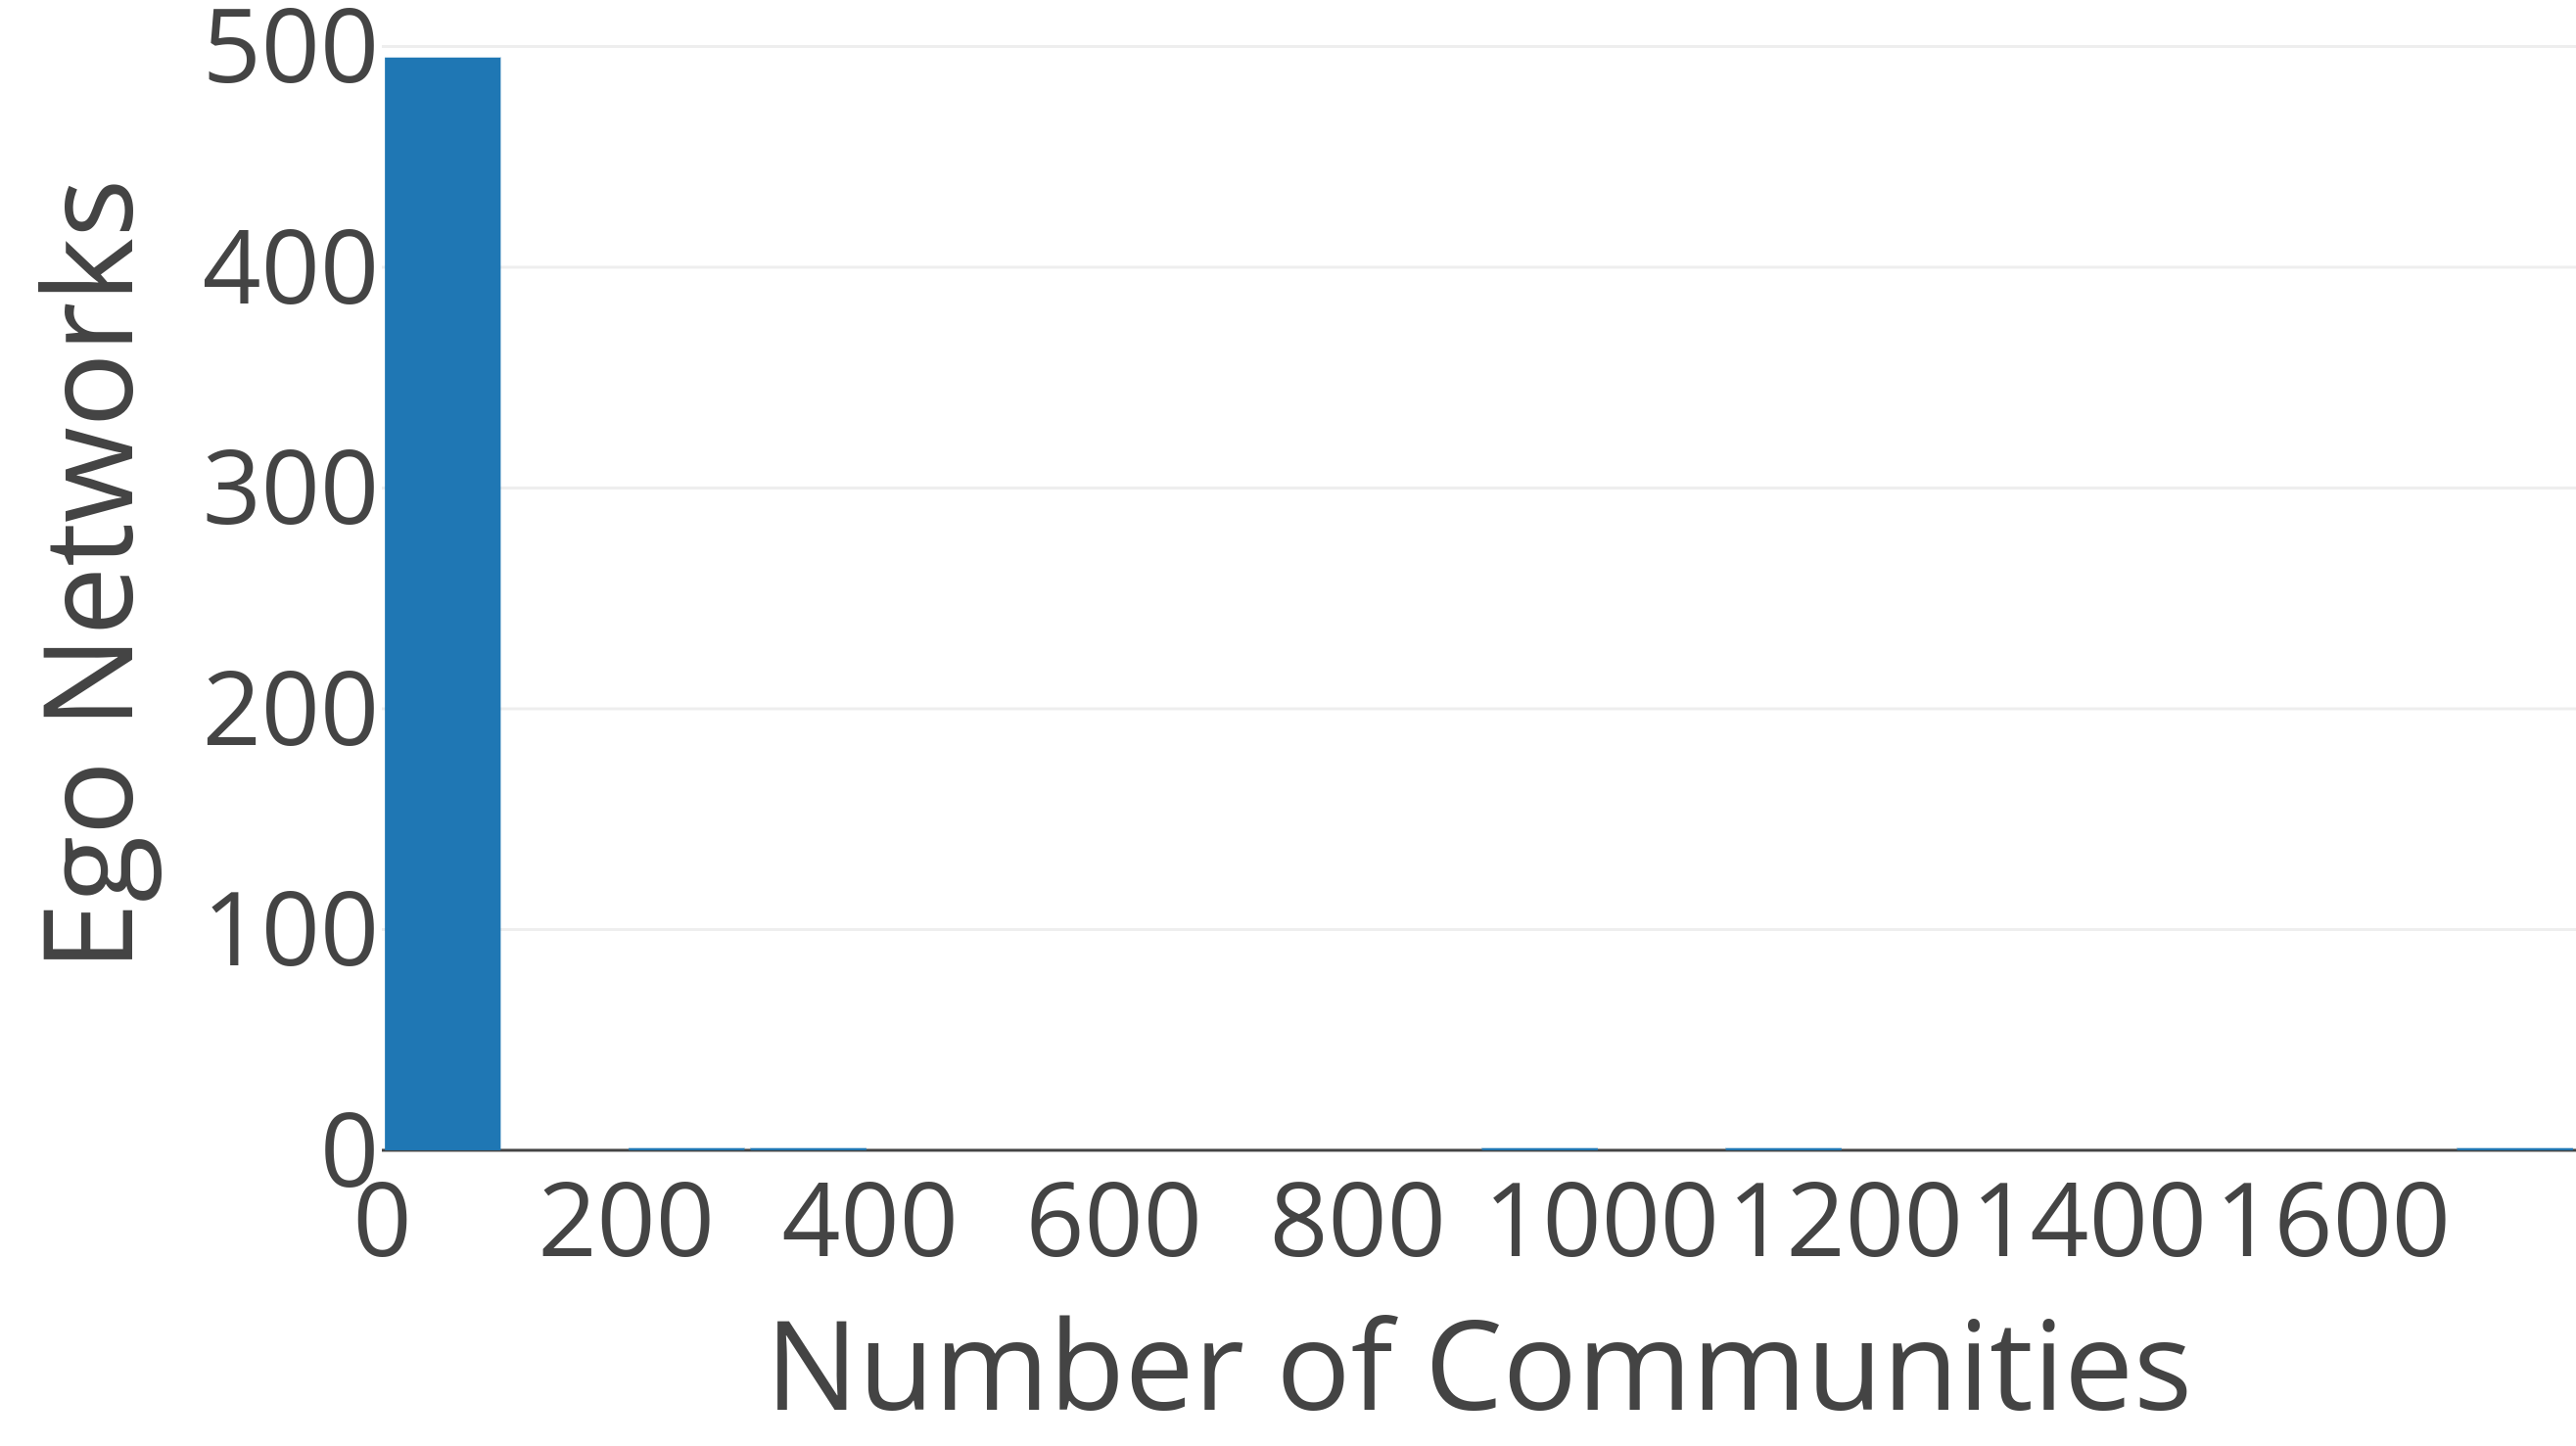
\includegraphics[width=0.47\textwidth]{fig/comm_stats/rak/n_comm/n_comm_rak_follow.png}
        \label{fig:comm_stats_n_comm_rak_follow}
    }
    \subfigure[Retweet]{
        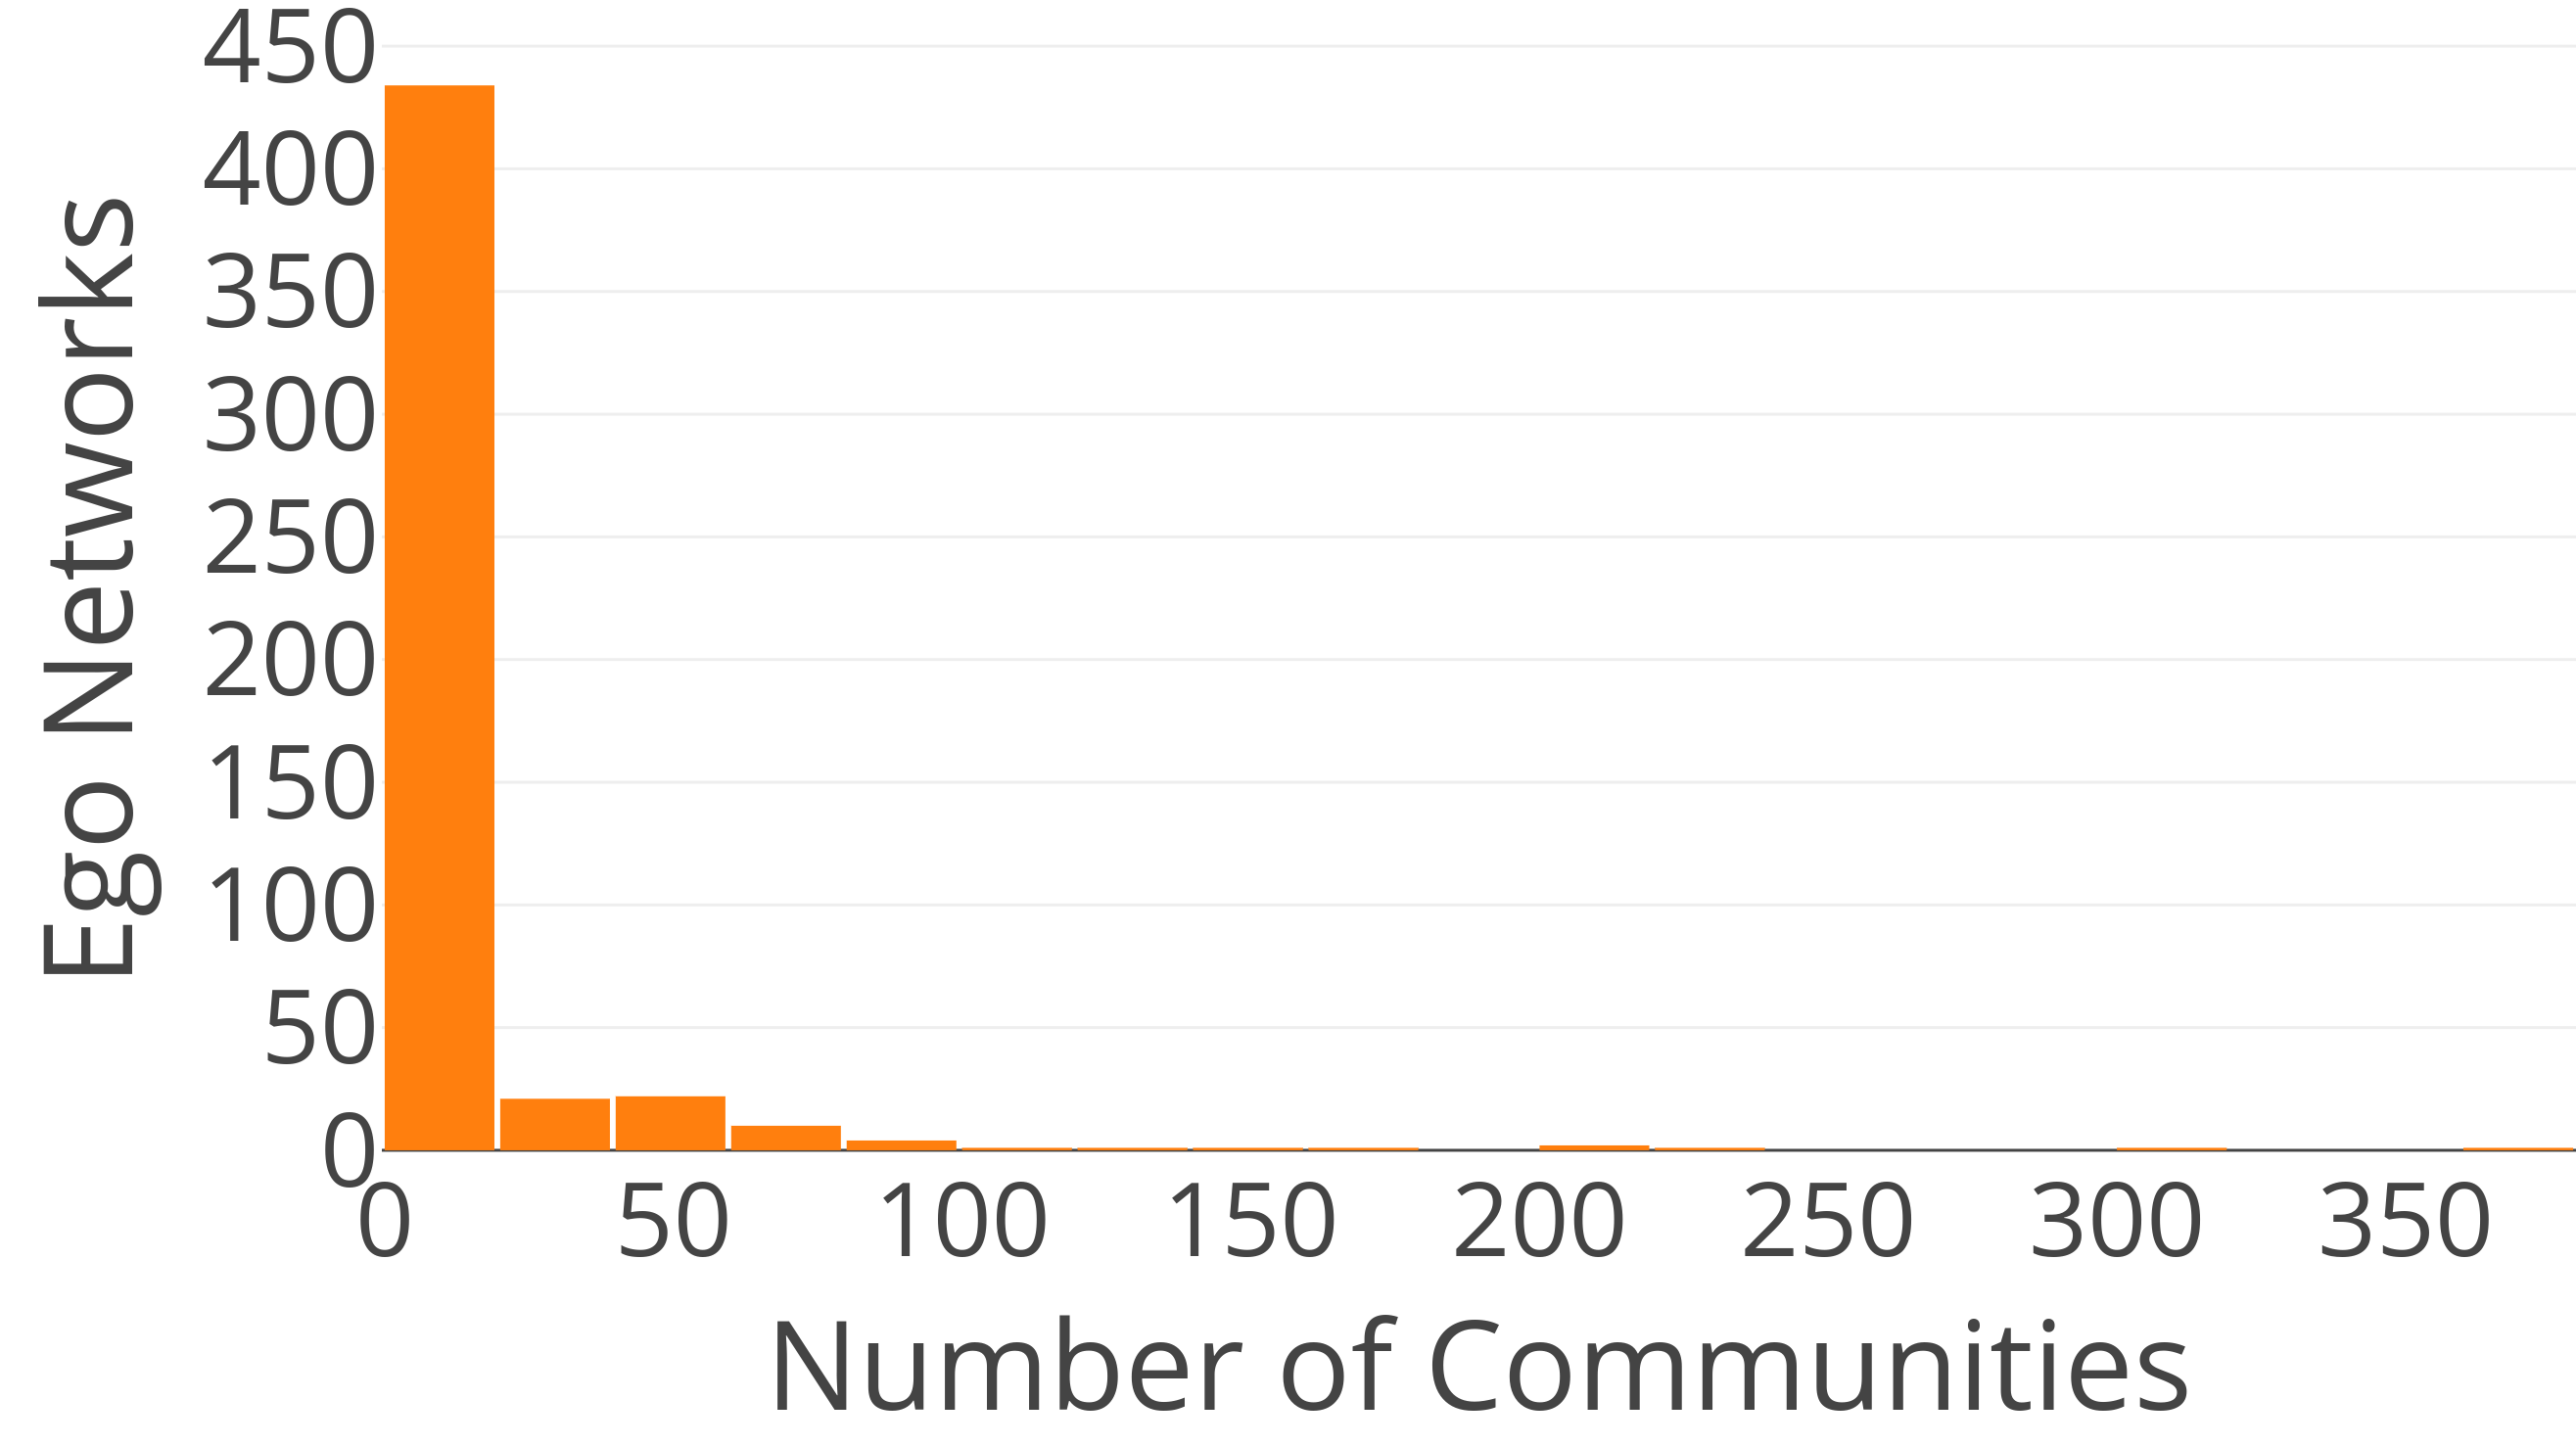
\includegraphics[width=0.47\textwidth]{fig/comm_stats/rak/n_comm/n_comm_rak_retweet.png}
        \label{fig:comm_stats_n_comm_rak_retweet}
    } \\
    \subfigure[Like]{
        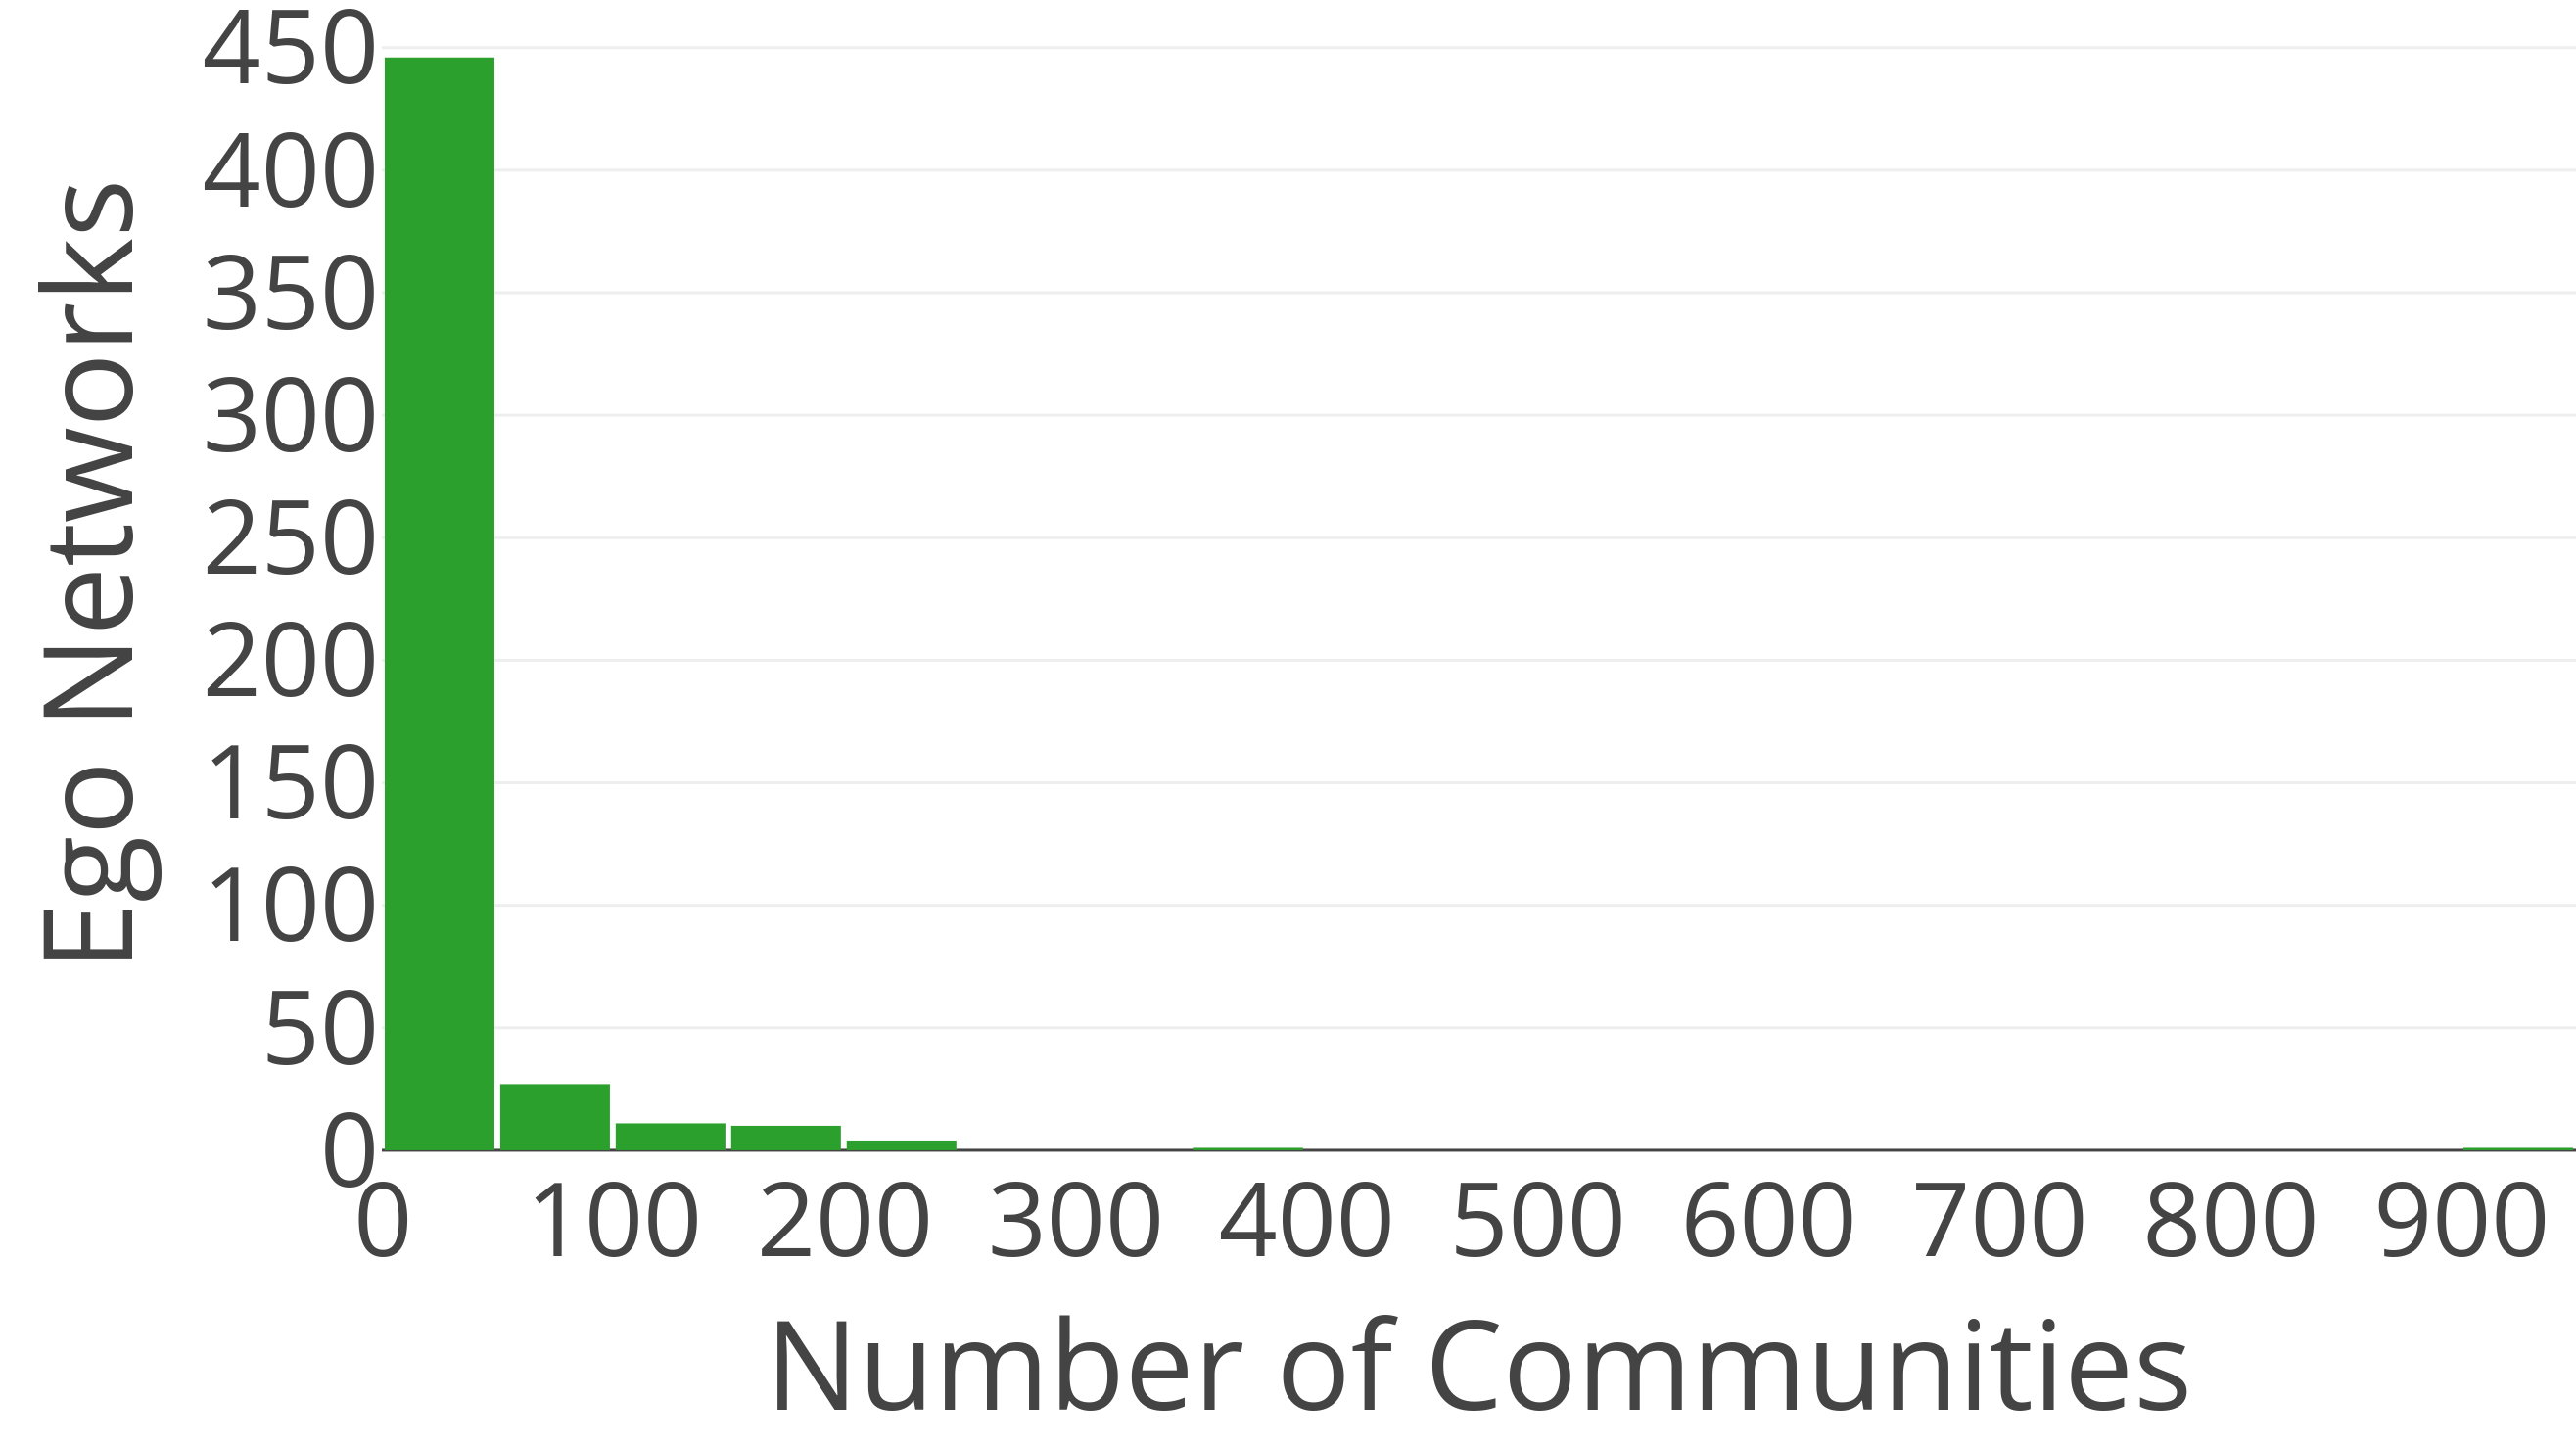
\includegraphics[width=0.47\textwidth]{fig/comm_stats/rak/n_comm/n_comm_rak_like.png}
        \label{fig:comm_stats_n_comm_rak_like}
    }
    \subfigure[Mention]{
        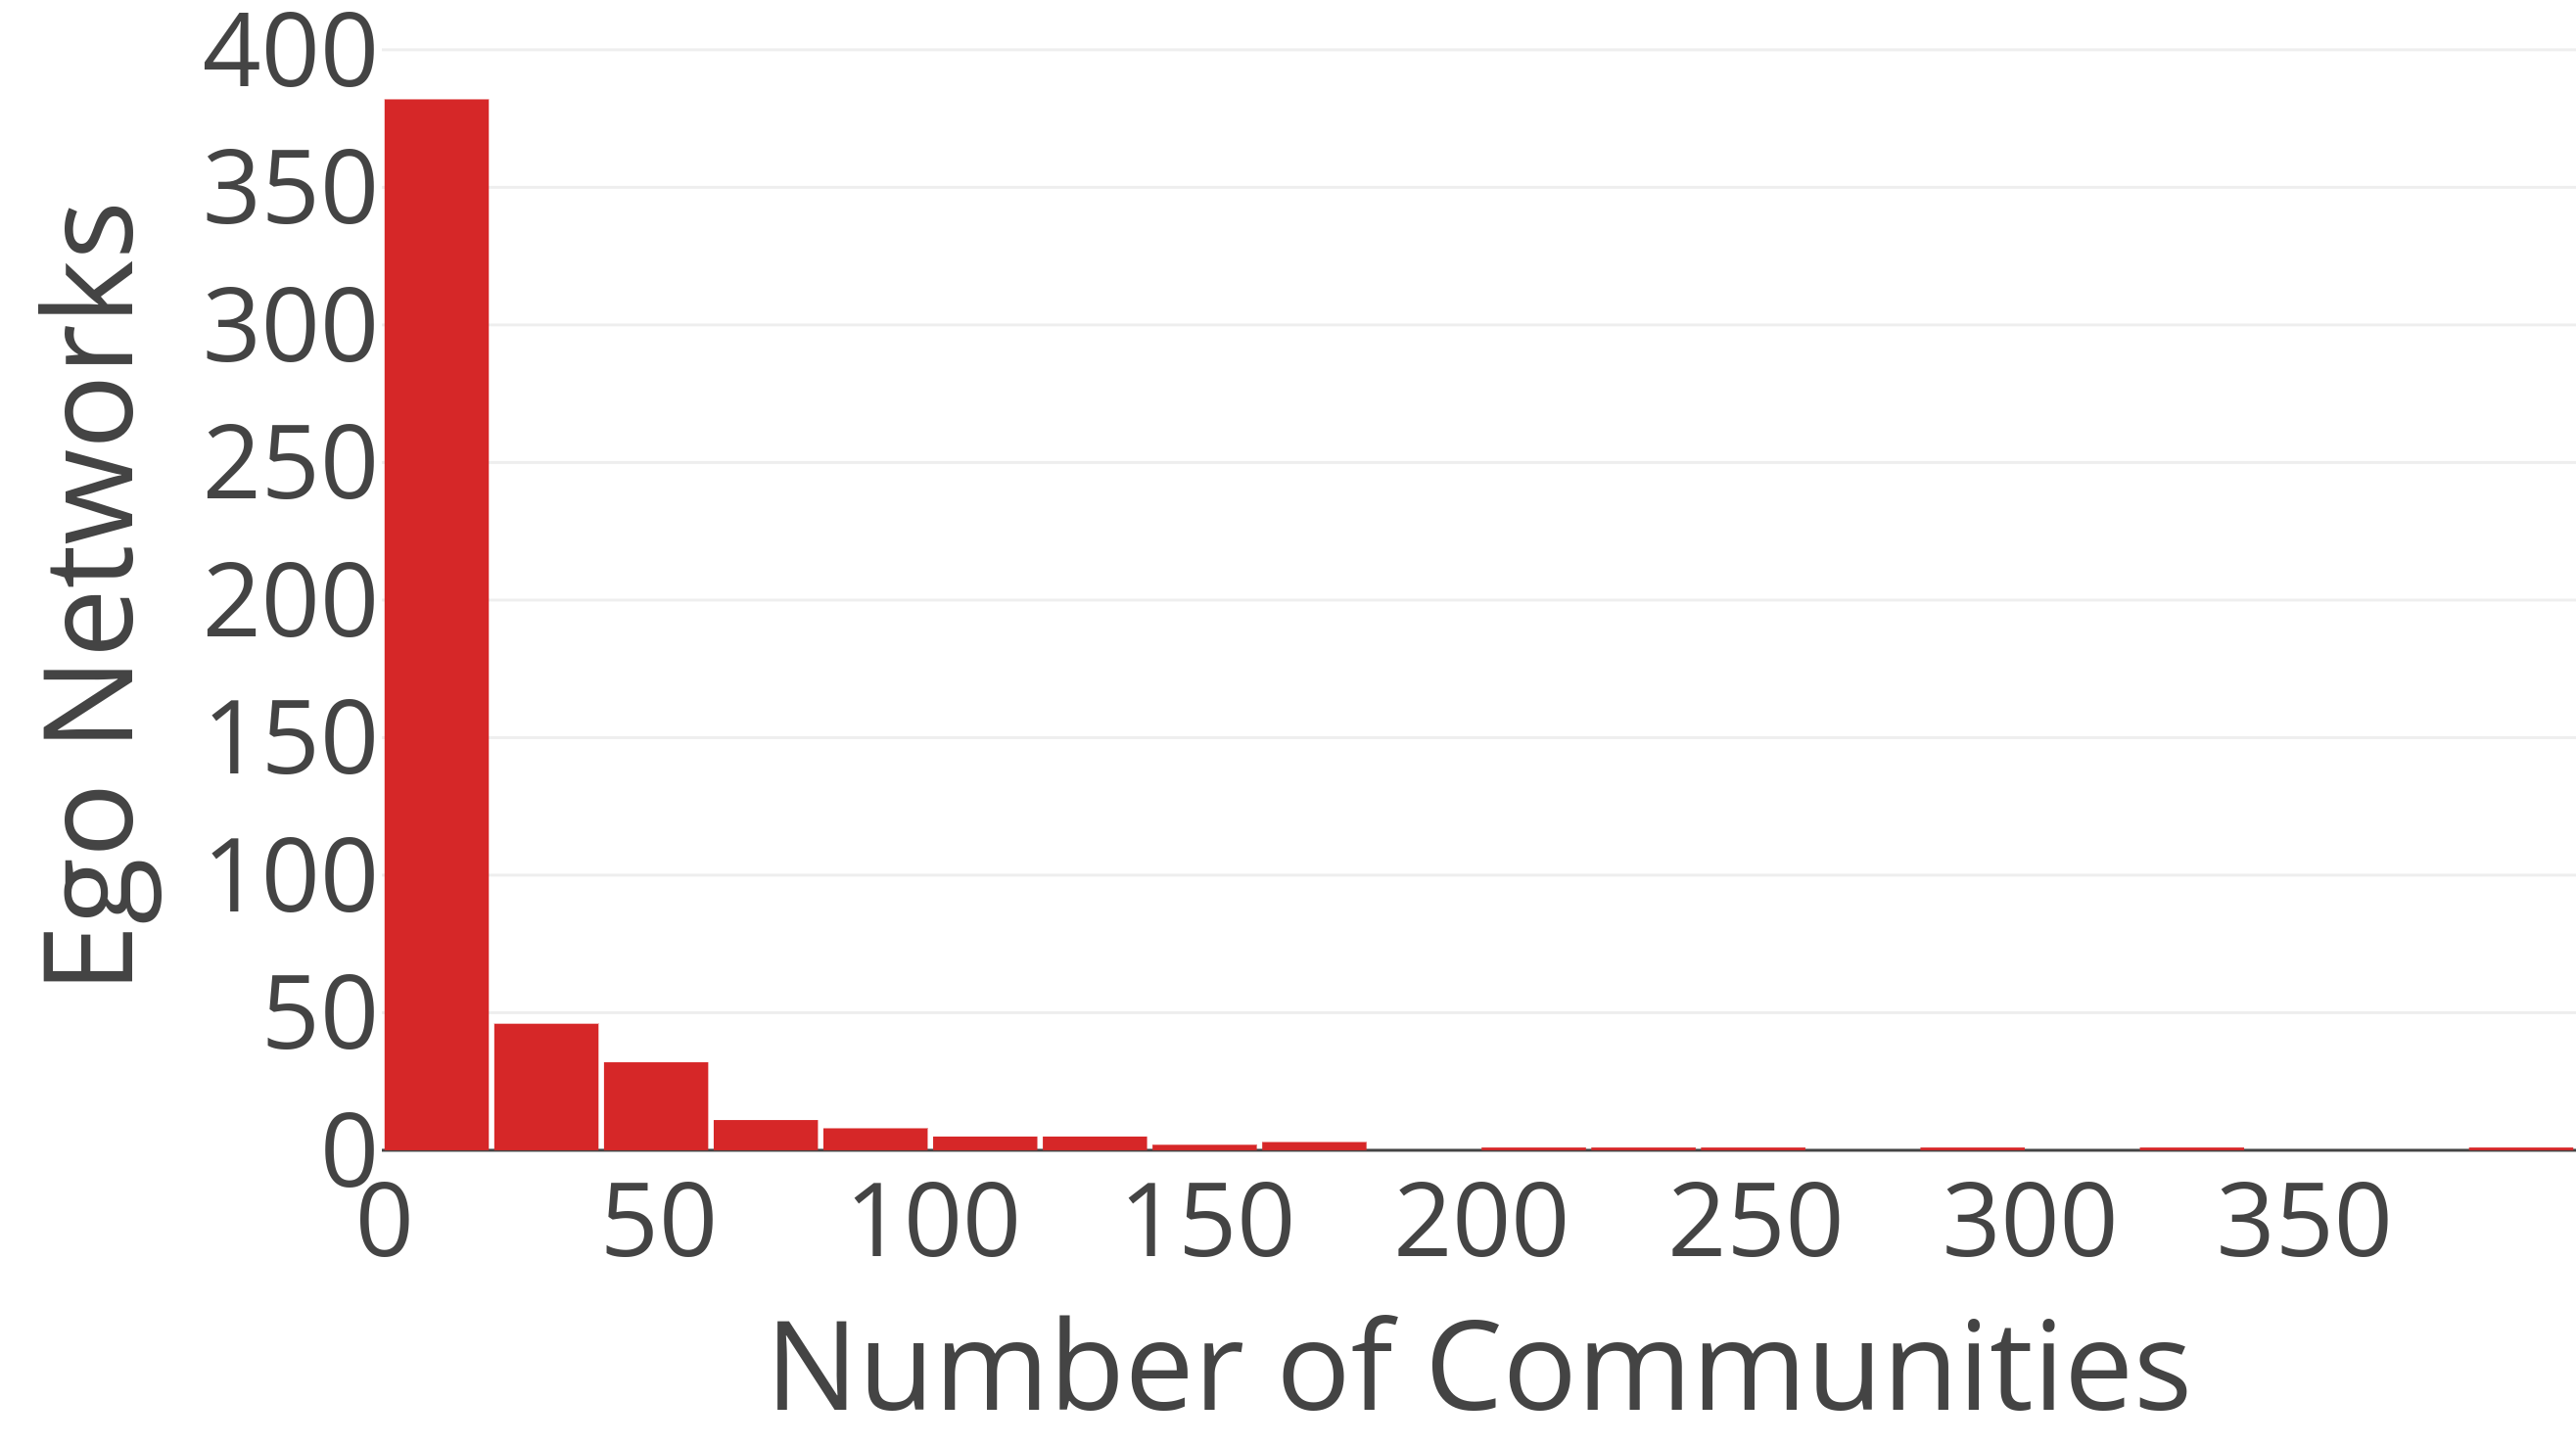
\includegraphics[width=0.47\textwidth]{fig/comm_stats/rak/n_comm/n_comm_rak_mention.png}
        \label{fig:comm_stats_n_comm_rak_mention}
    }
    \caption{Number of communities detected by RAK.}
    \label{fig:comm_stats_n_comm_rak}
    
\end{figure}

\begin{figure}[h!tb]
    \centering
    \subfigure[Follow]{
        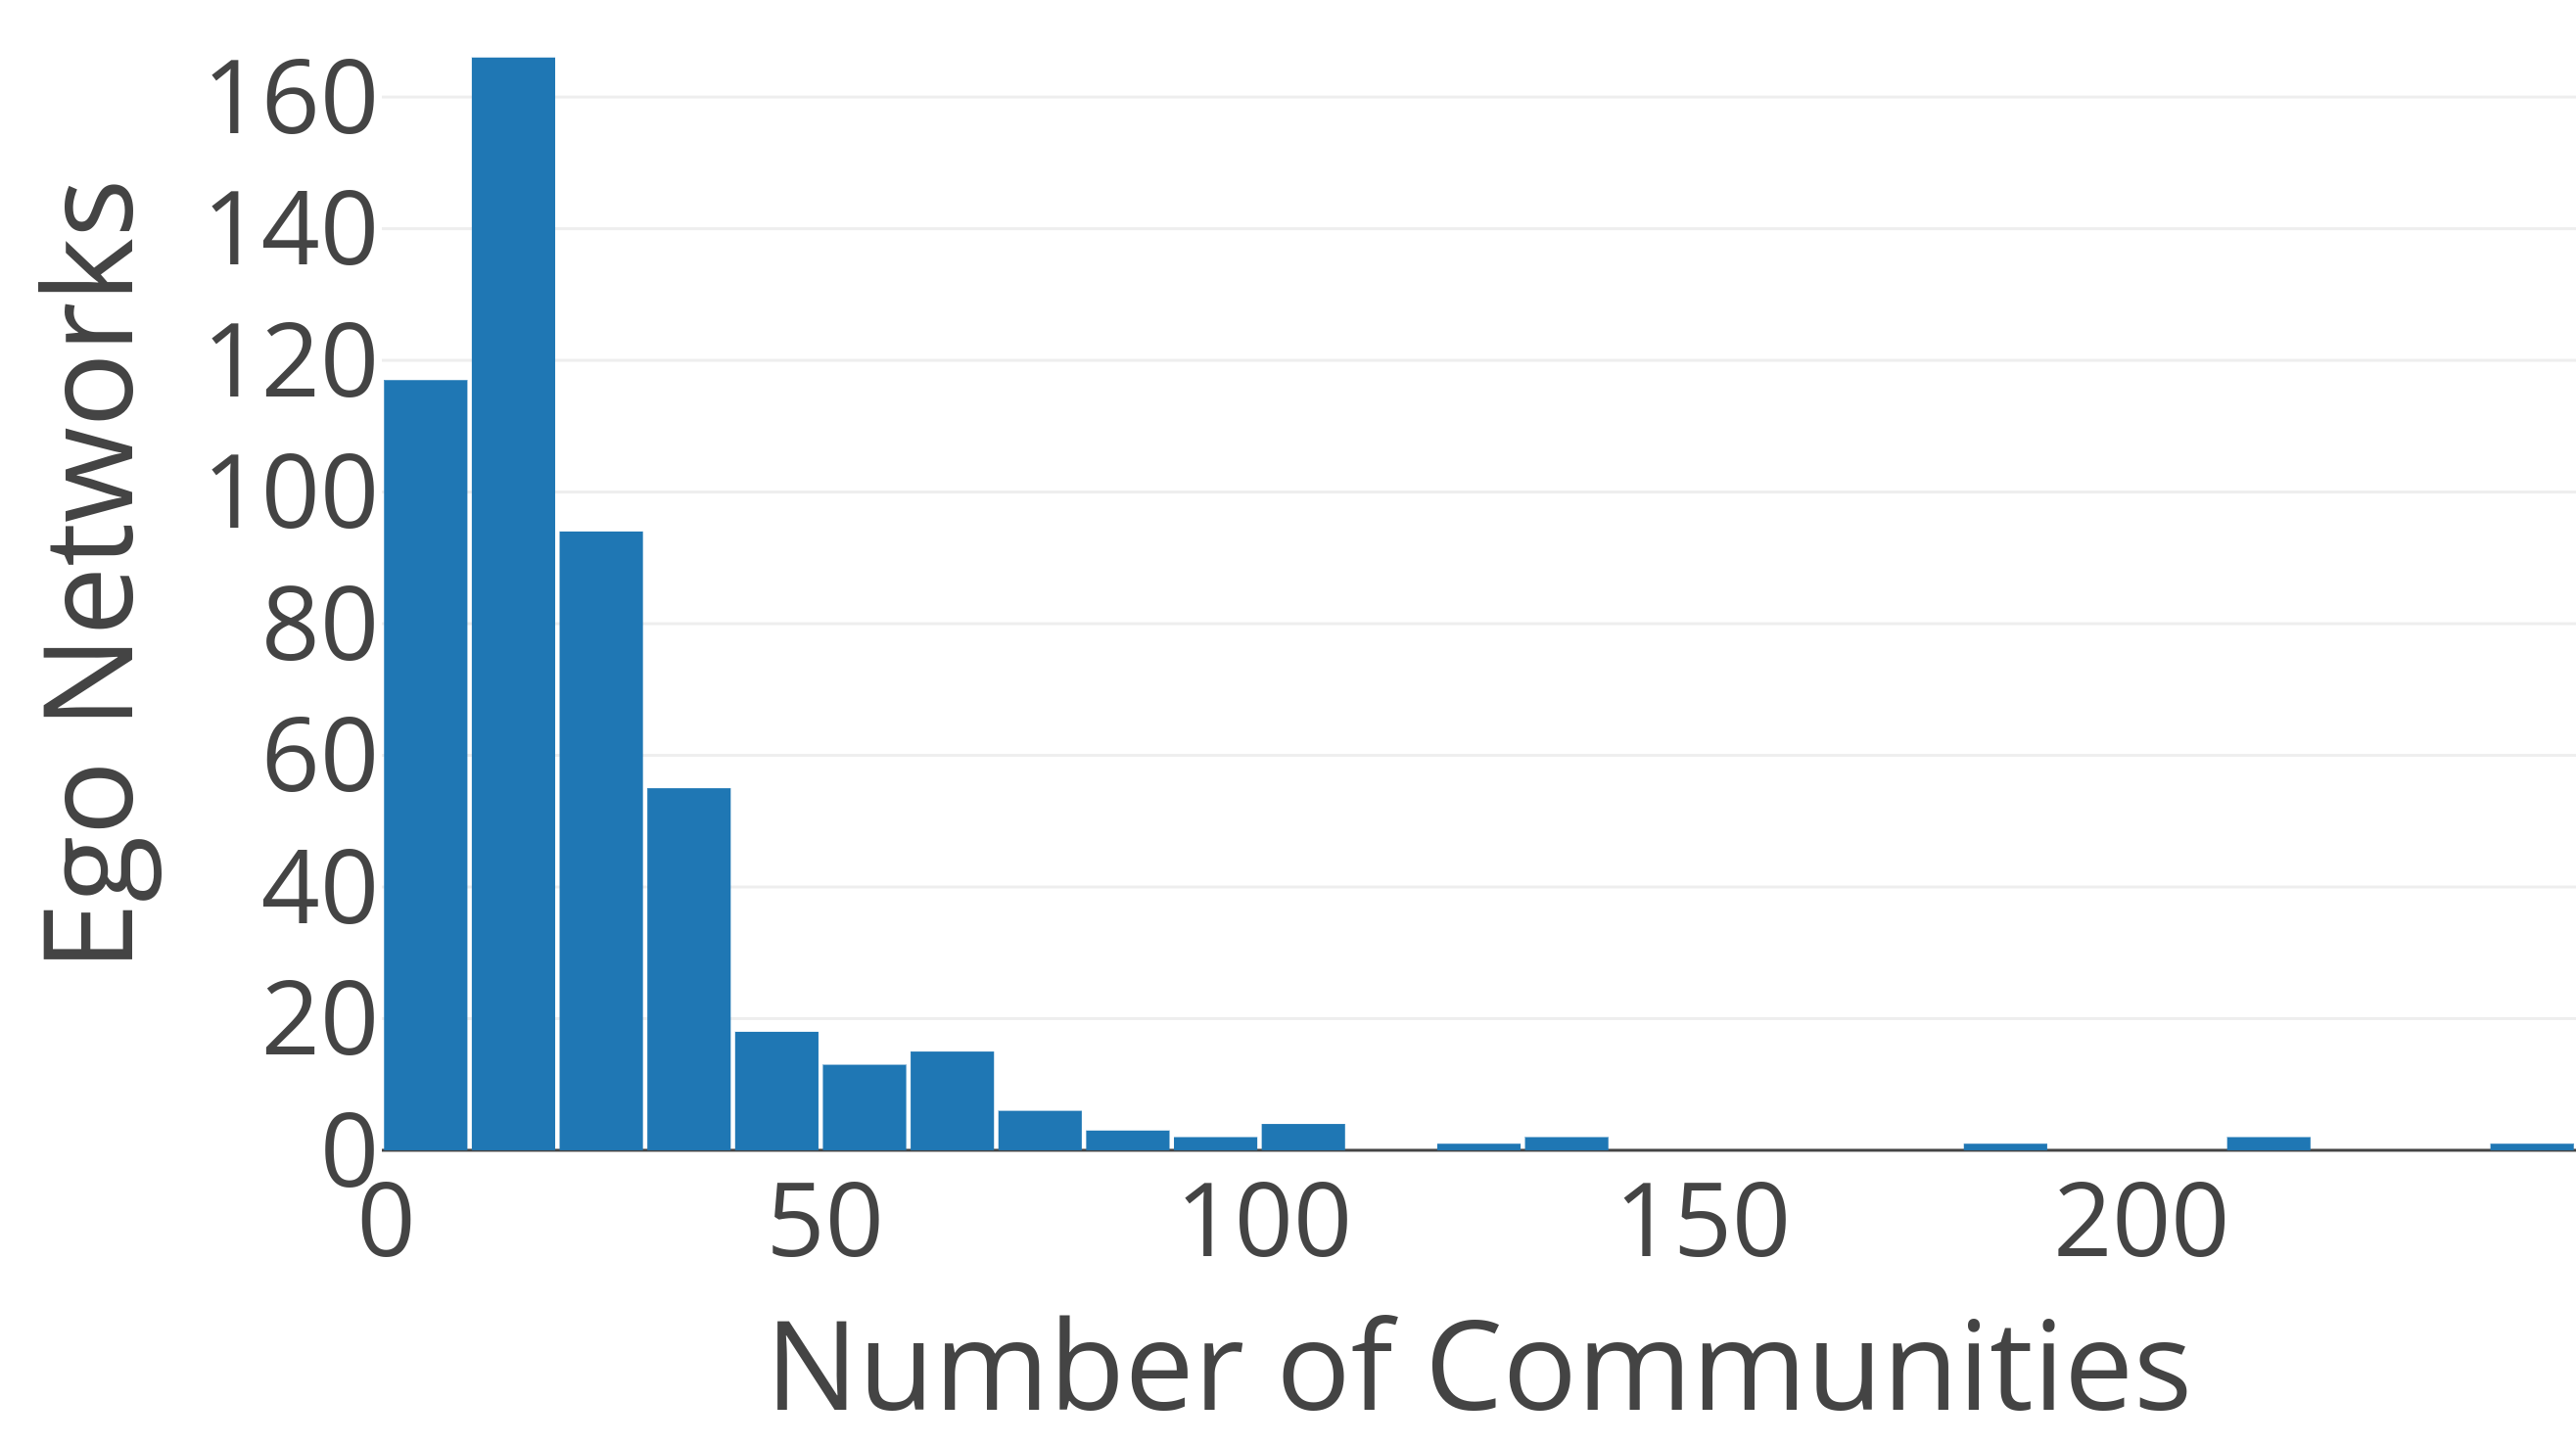
\includegraphics[width=0.47\textwidth]{fig/comm_stats/infomap/n_comm/n_comm_infomap_follow.png}
        \label{fig:comm_stats_n_comm_infomap_follow}
    }
    \subfigure[Retweet]{
        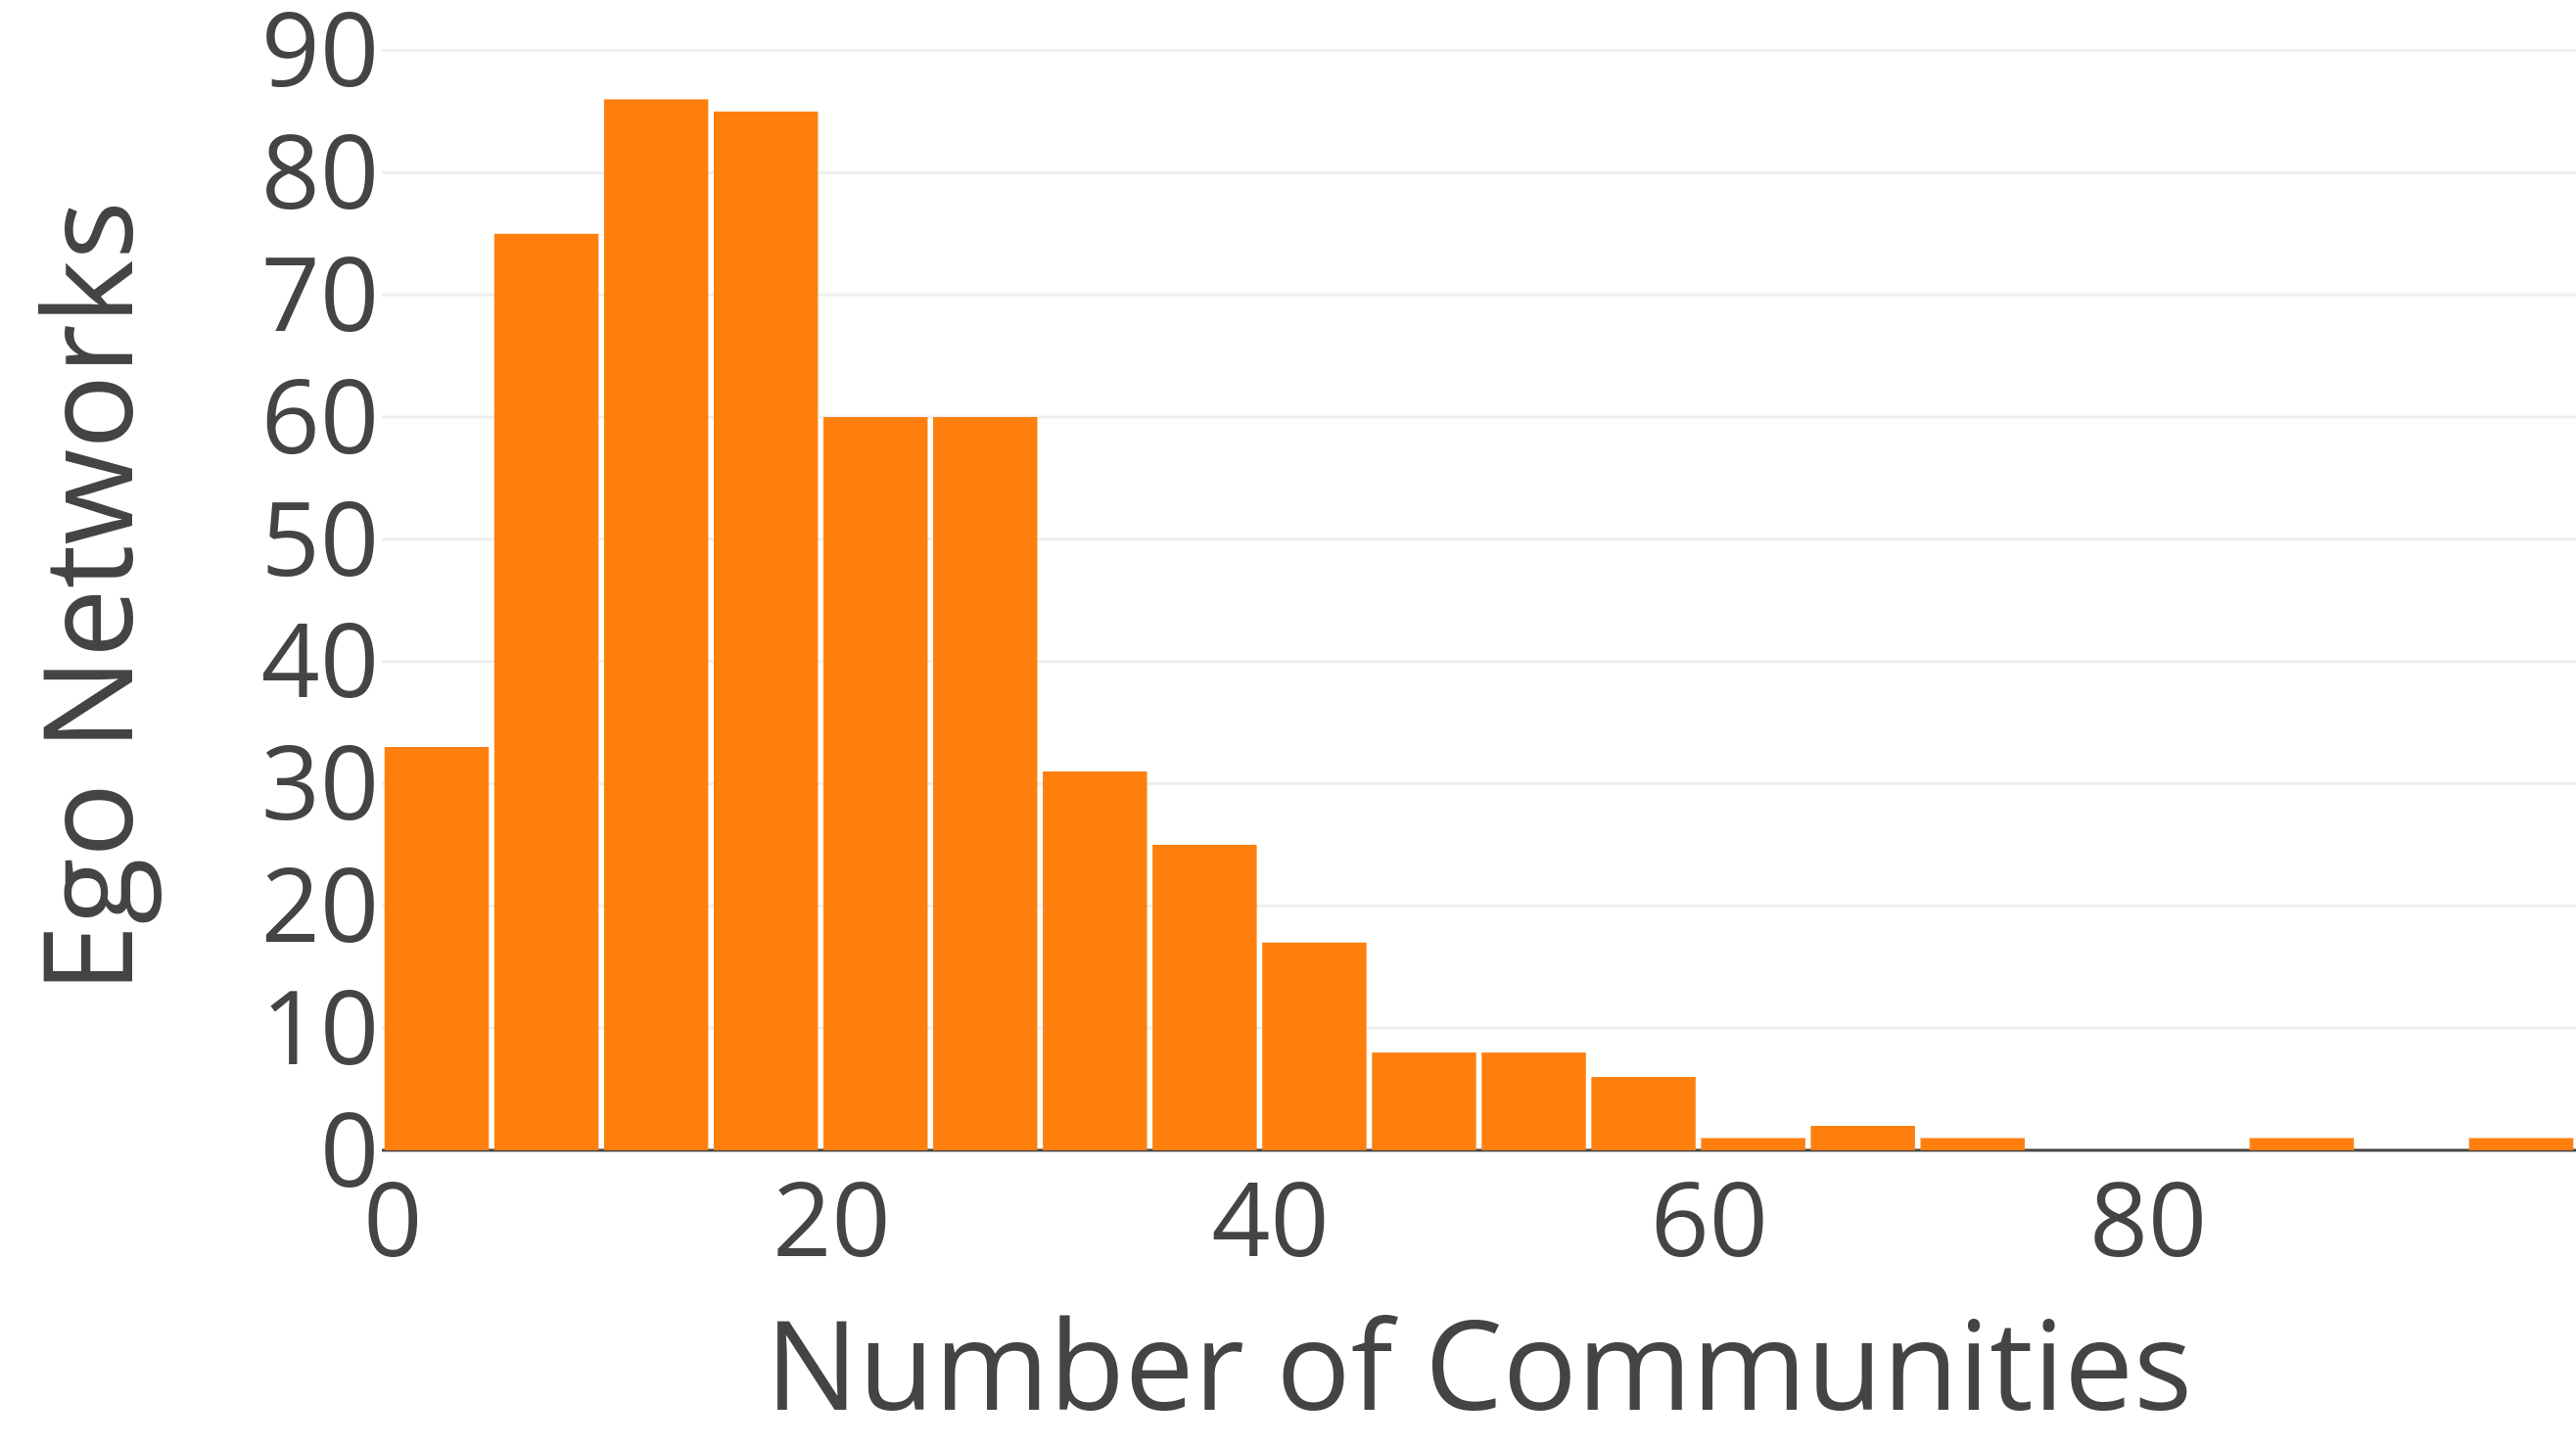
\includegraphics[width=0.47\textwidth]{fig/comm_stats/infomap/n_comm/n_comm_infomap_retweet.png}
        \label{fig:comm_stats_n_comm_infomap_retweet}
    } \\
    \subfigure[Like]{
        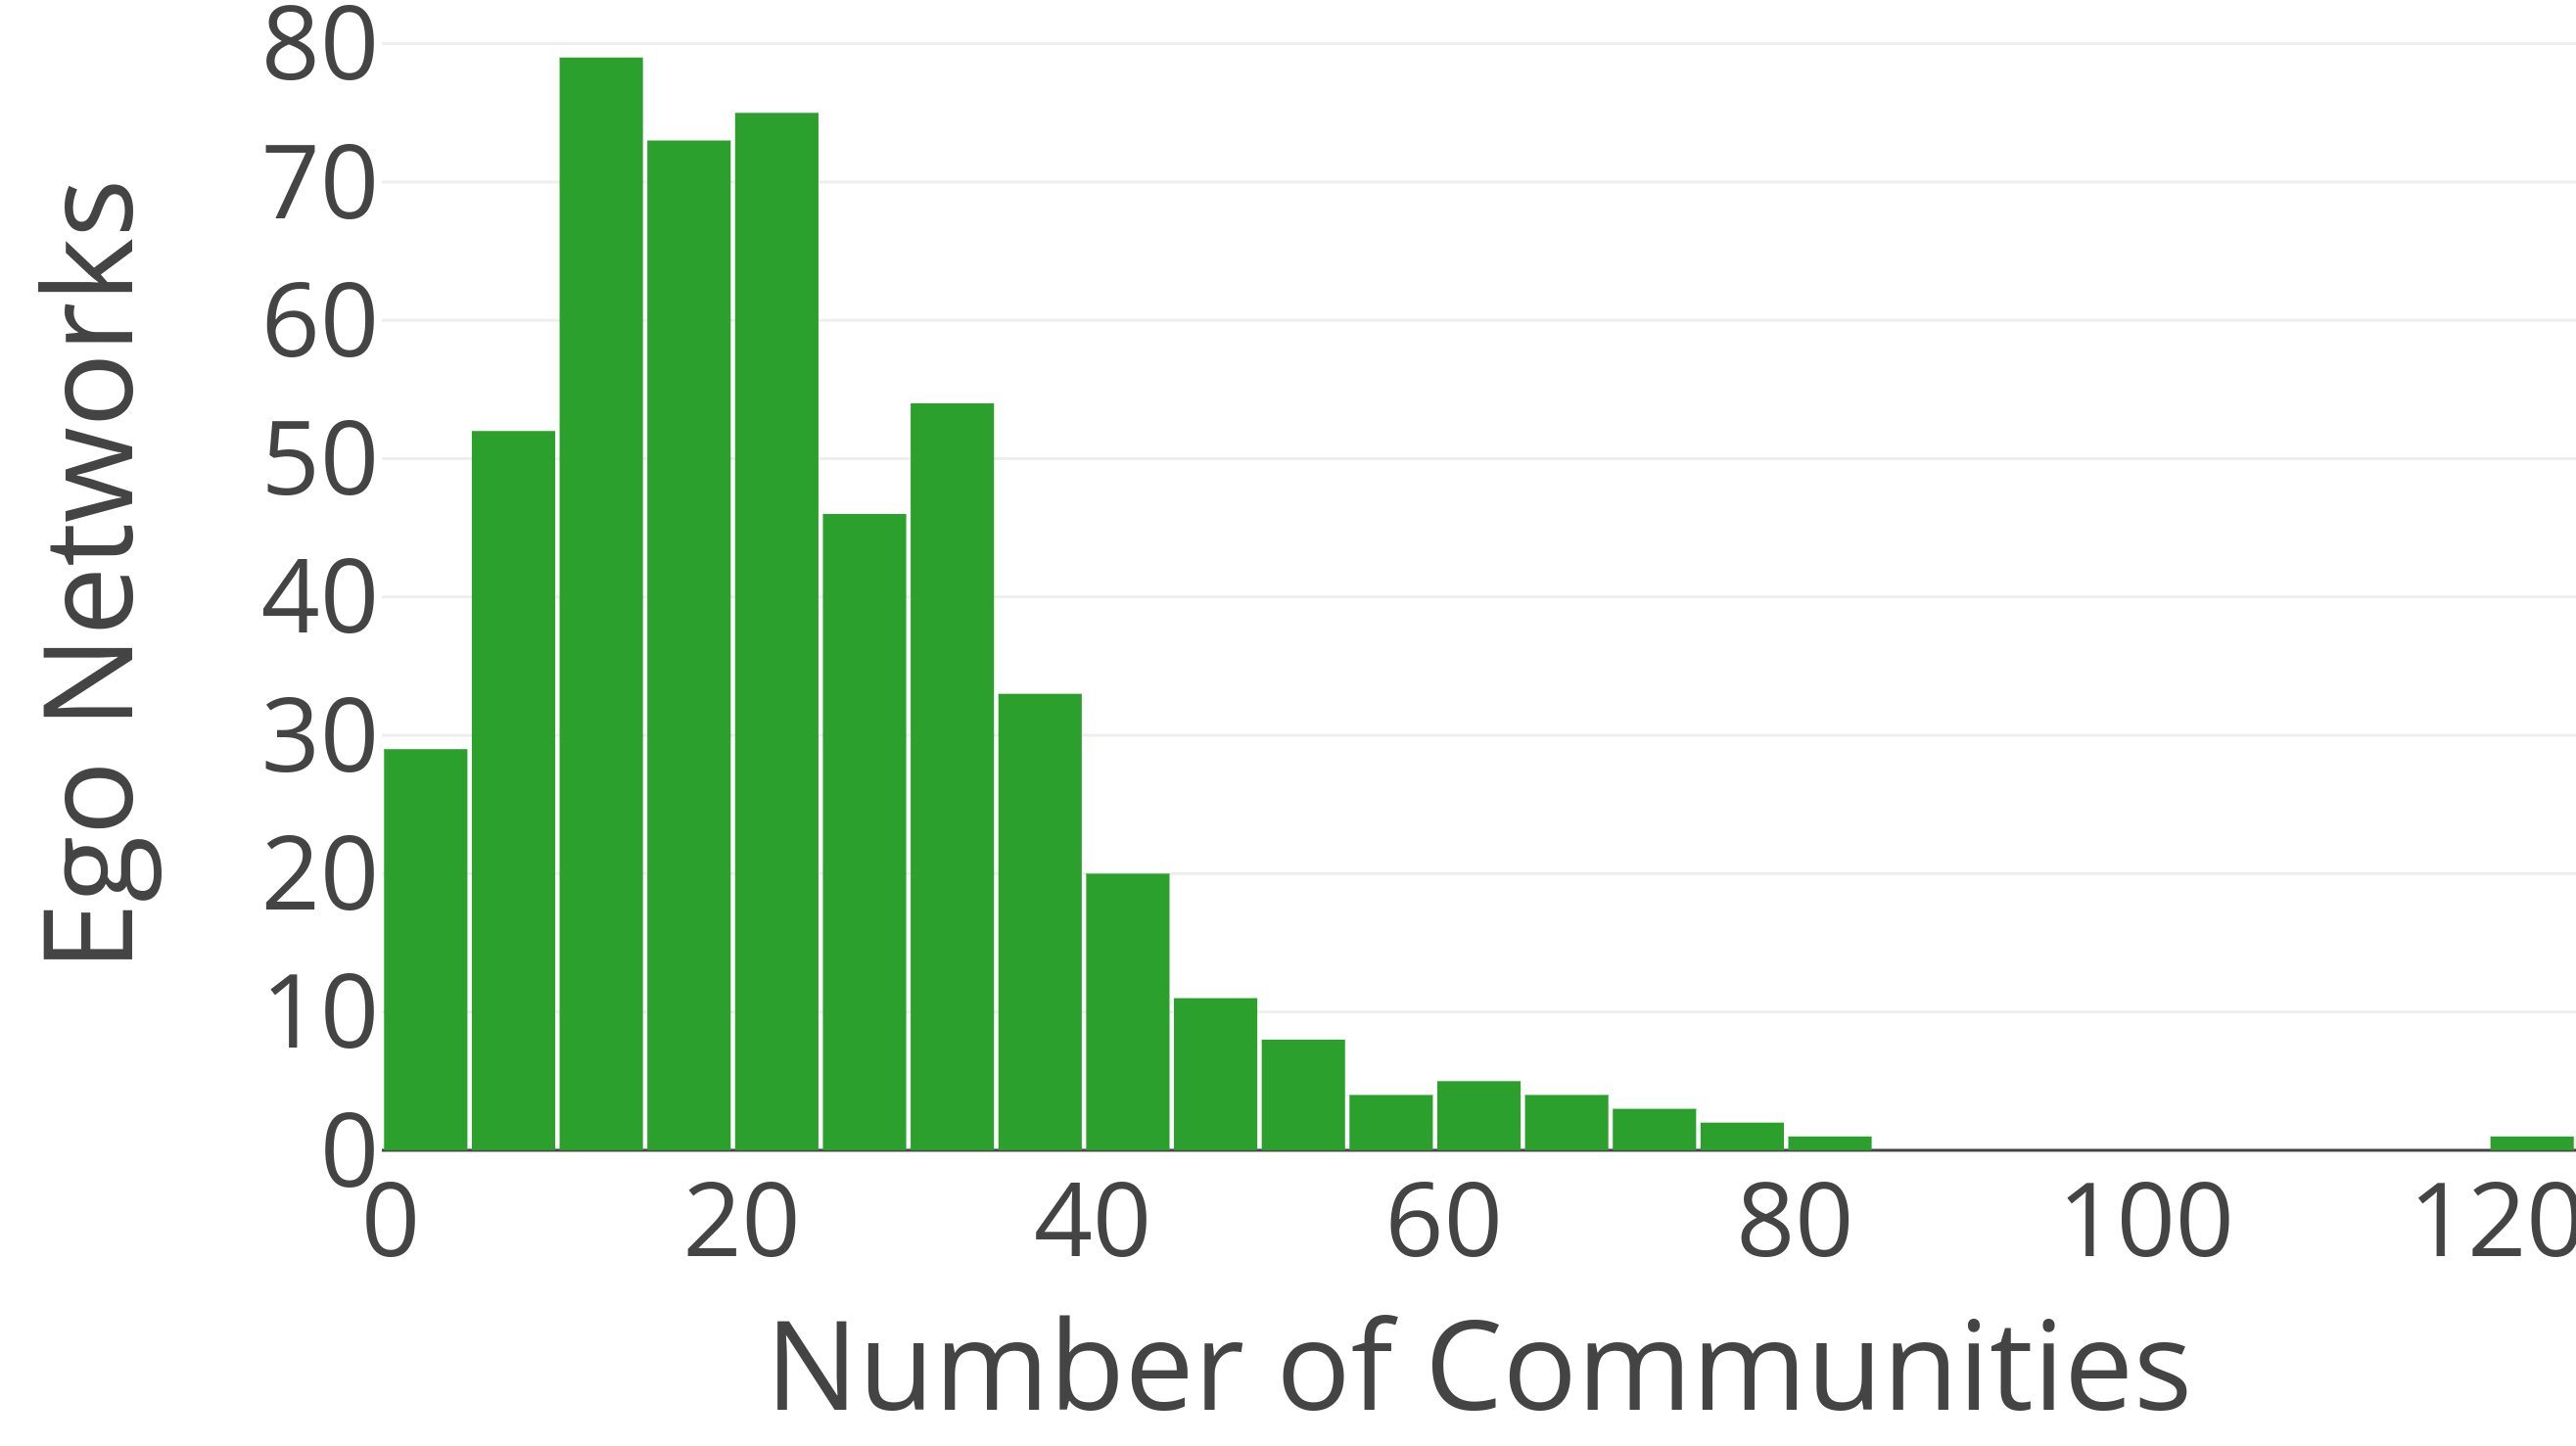
\includegraphics[width=0.47\textwidth]{fig/comm_stats/infomap/n_comm/n_comm_infomap_like.png}
        \label{fig:comm_stats_n_comm_infomap_like}
    }
    \subfigure[Mention]{
        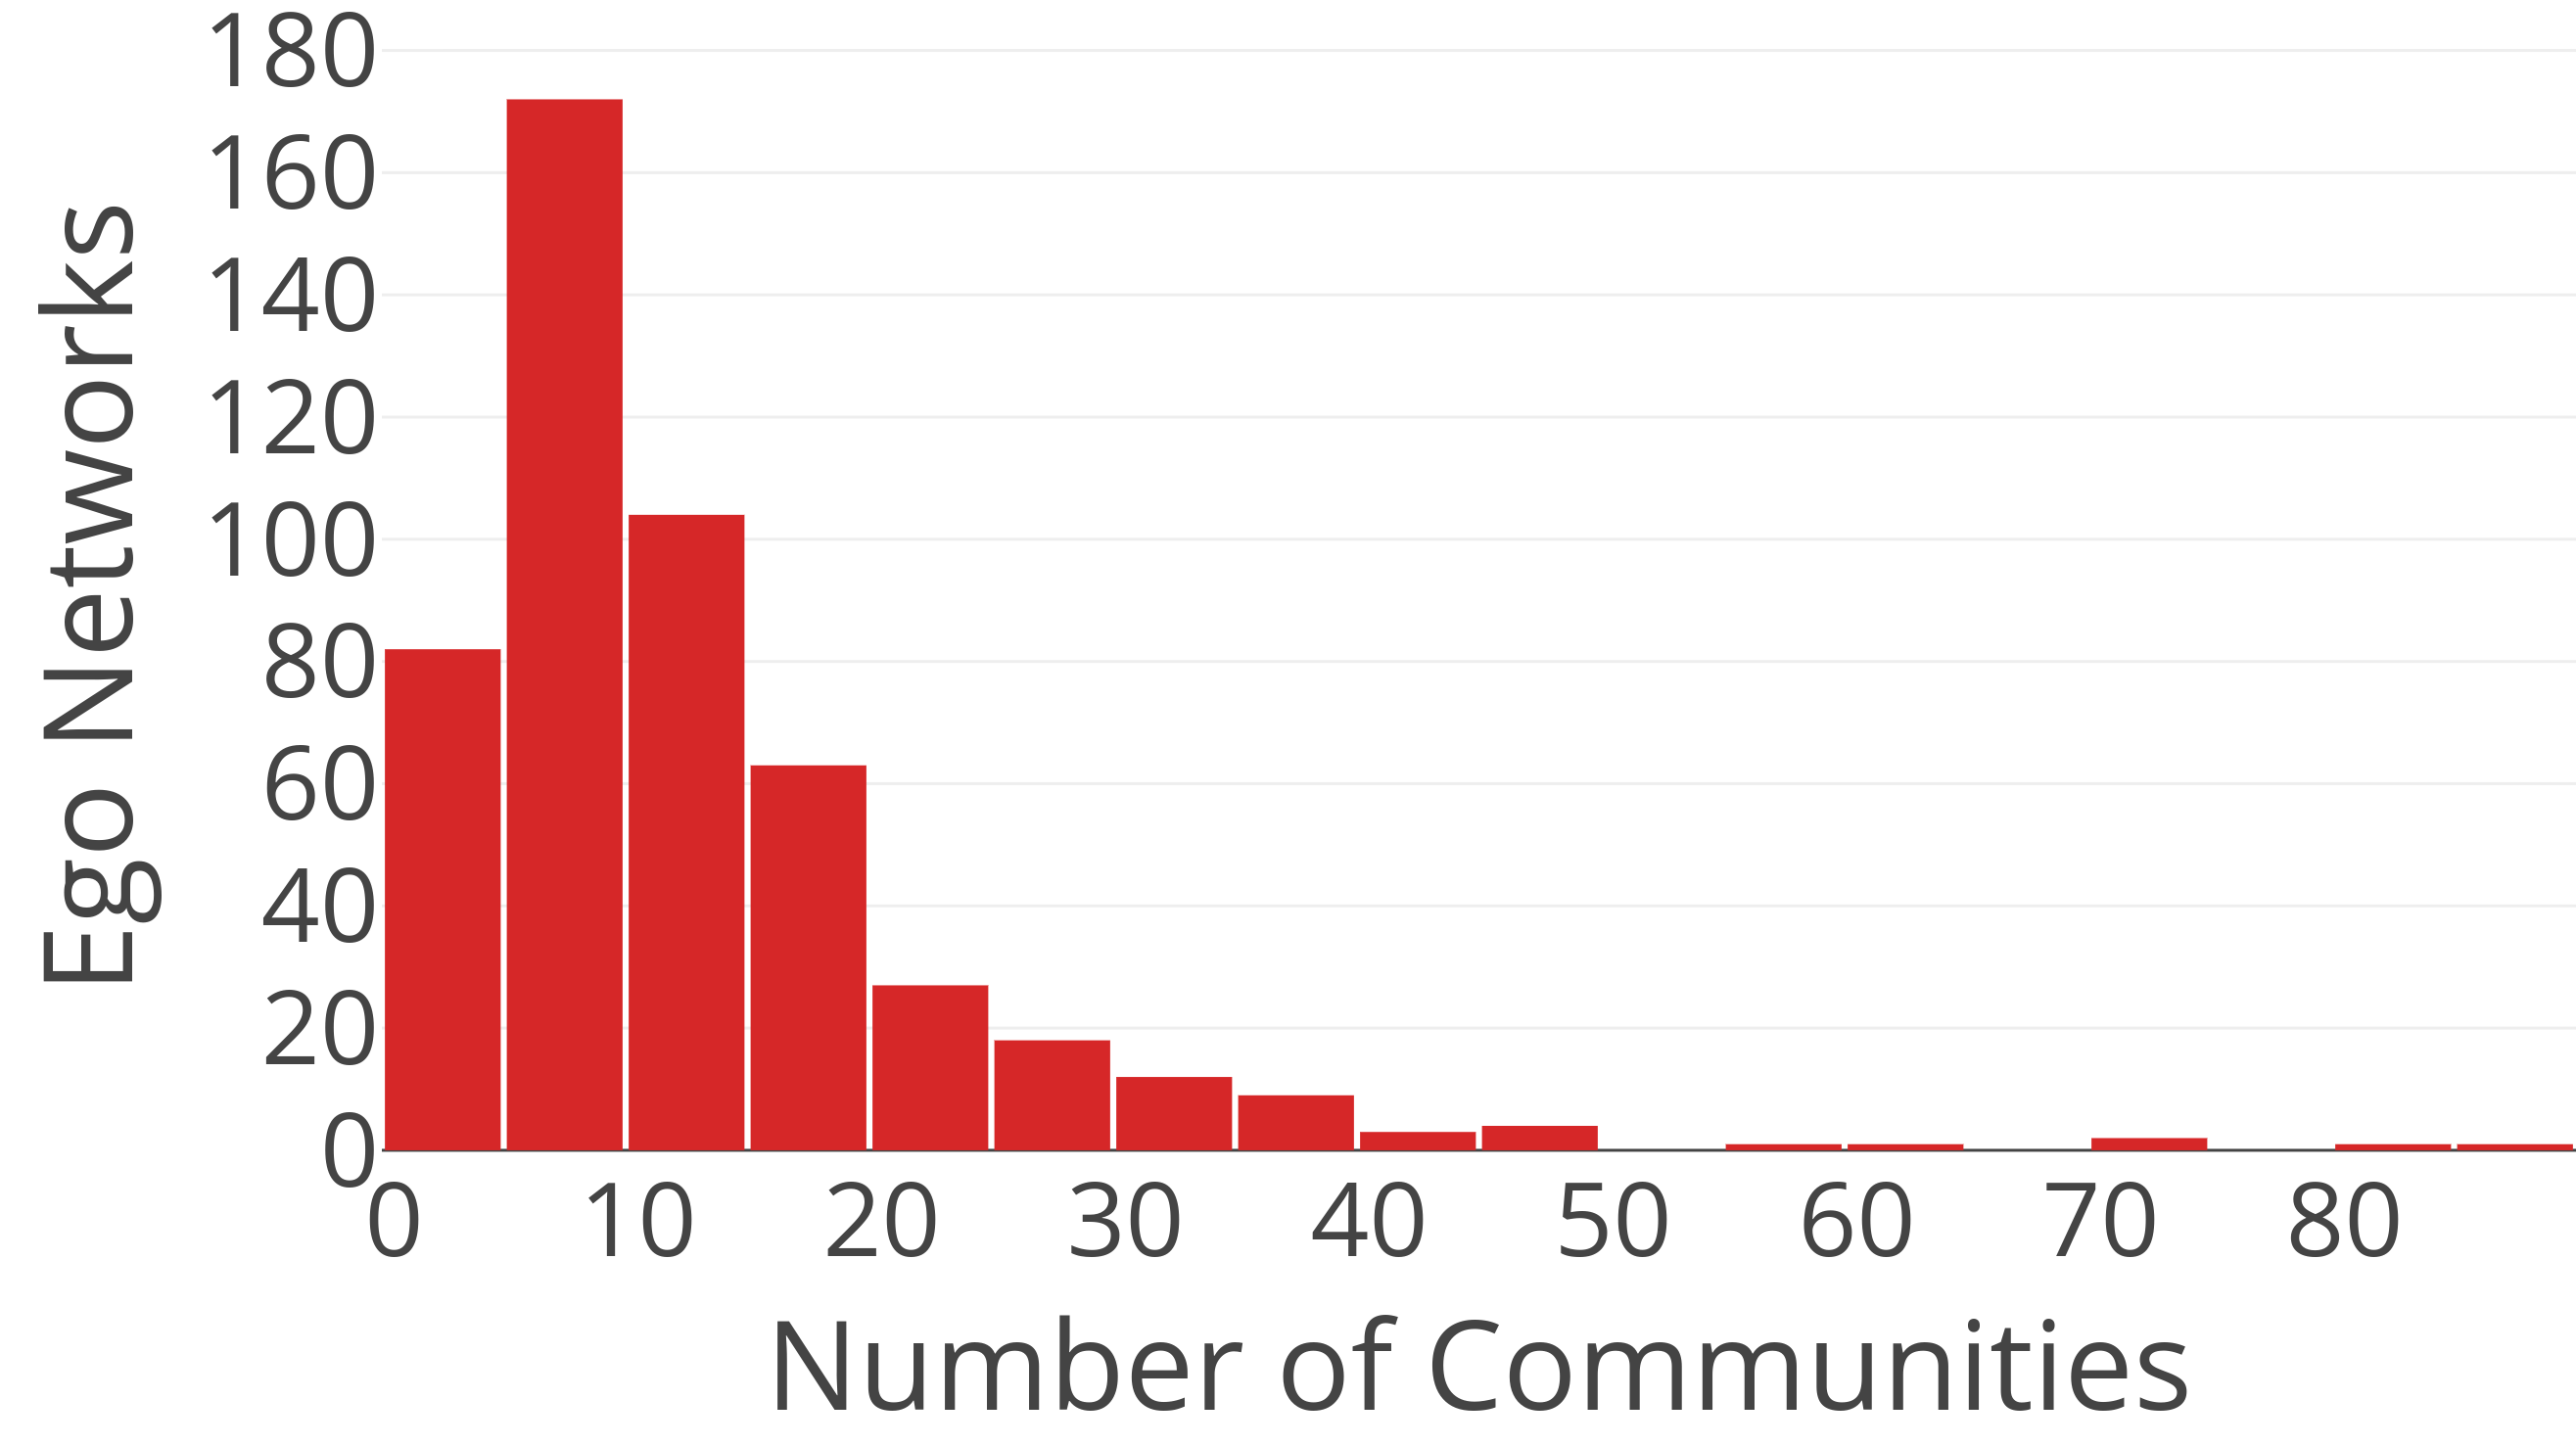
\includegraphics[width=0.47\textwidth]{fig/comm_stats/infomap/n_comm/n_comm_infomap_mention.png}
        \label{fig:comm_stats_n_comm_infomap_mention}
    }
    \caption{Number of communities detected by INFOMAP.}
    \label{fig:comm_stats_n_comm_infomap}
\end{figure}
\begin{figure}[h!tb]
    \centering
    \subfigure[Follow]{
        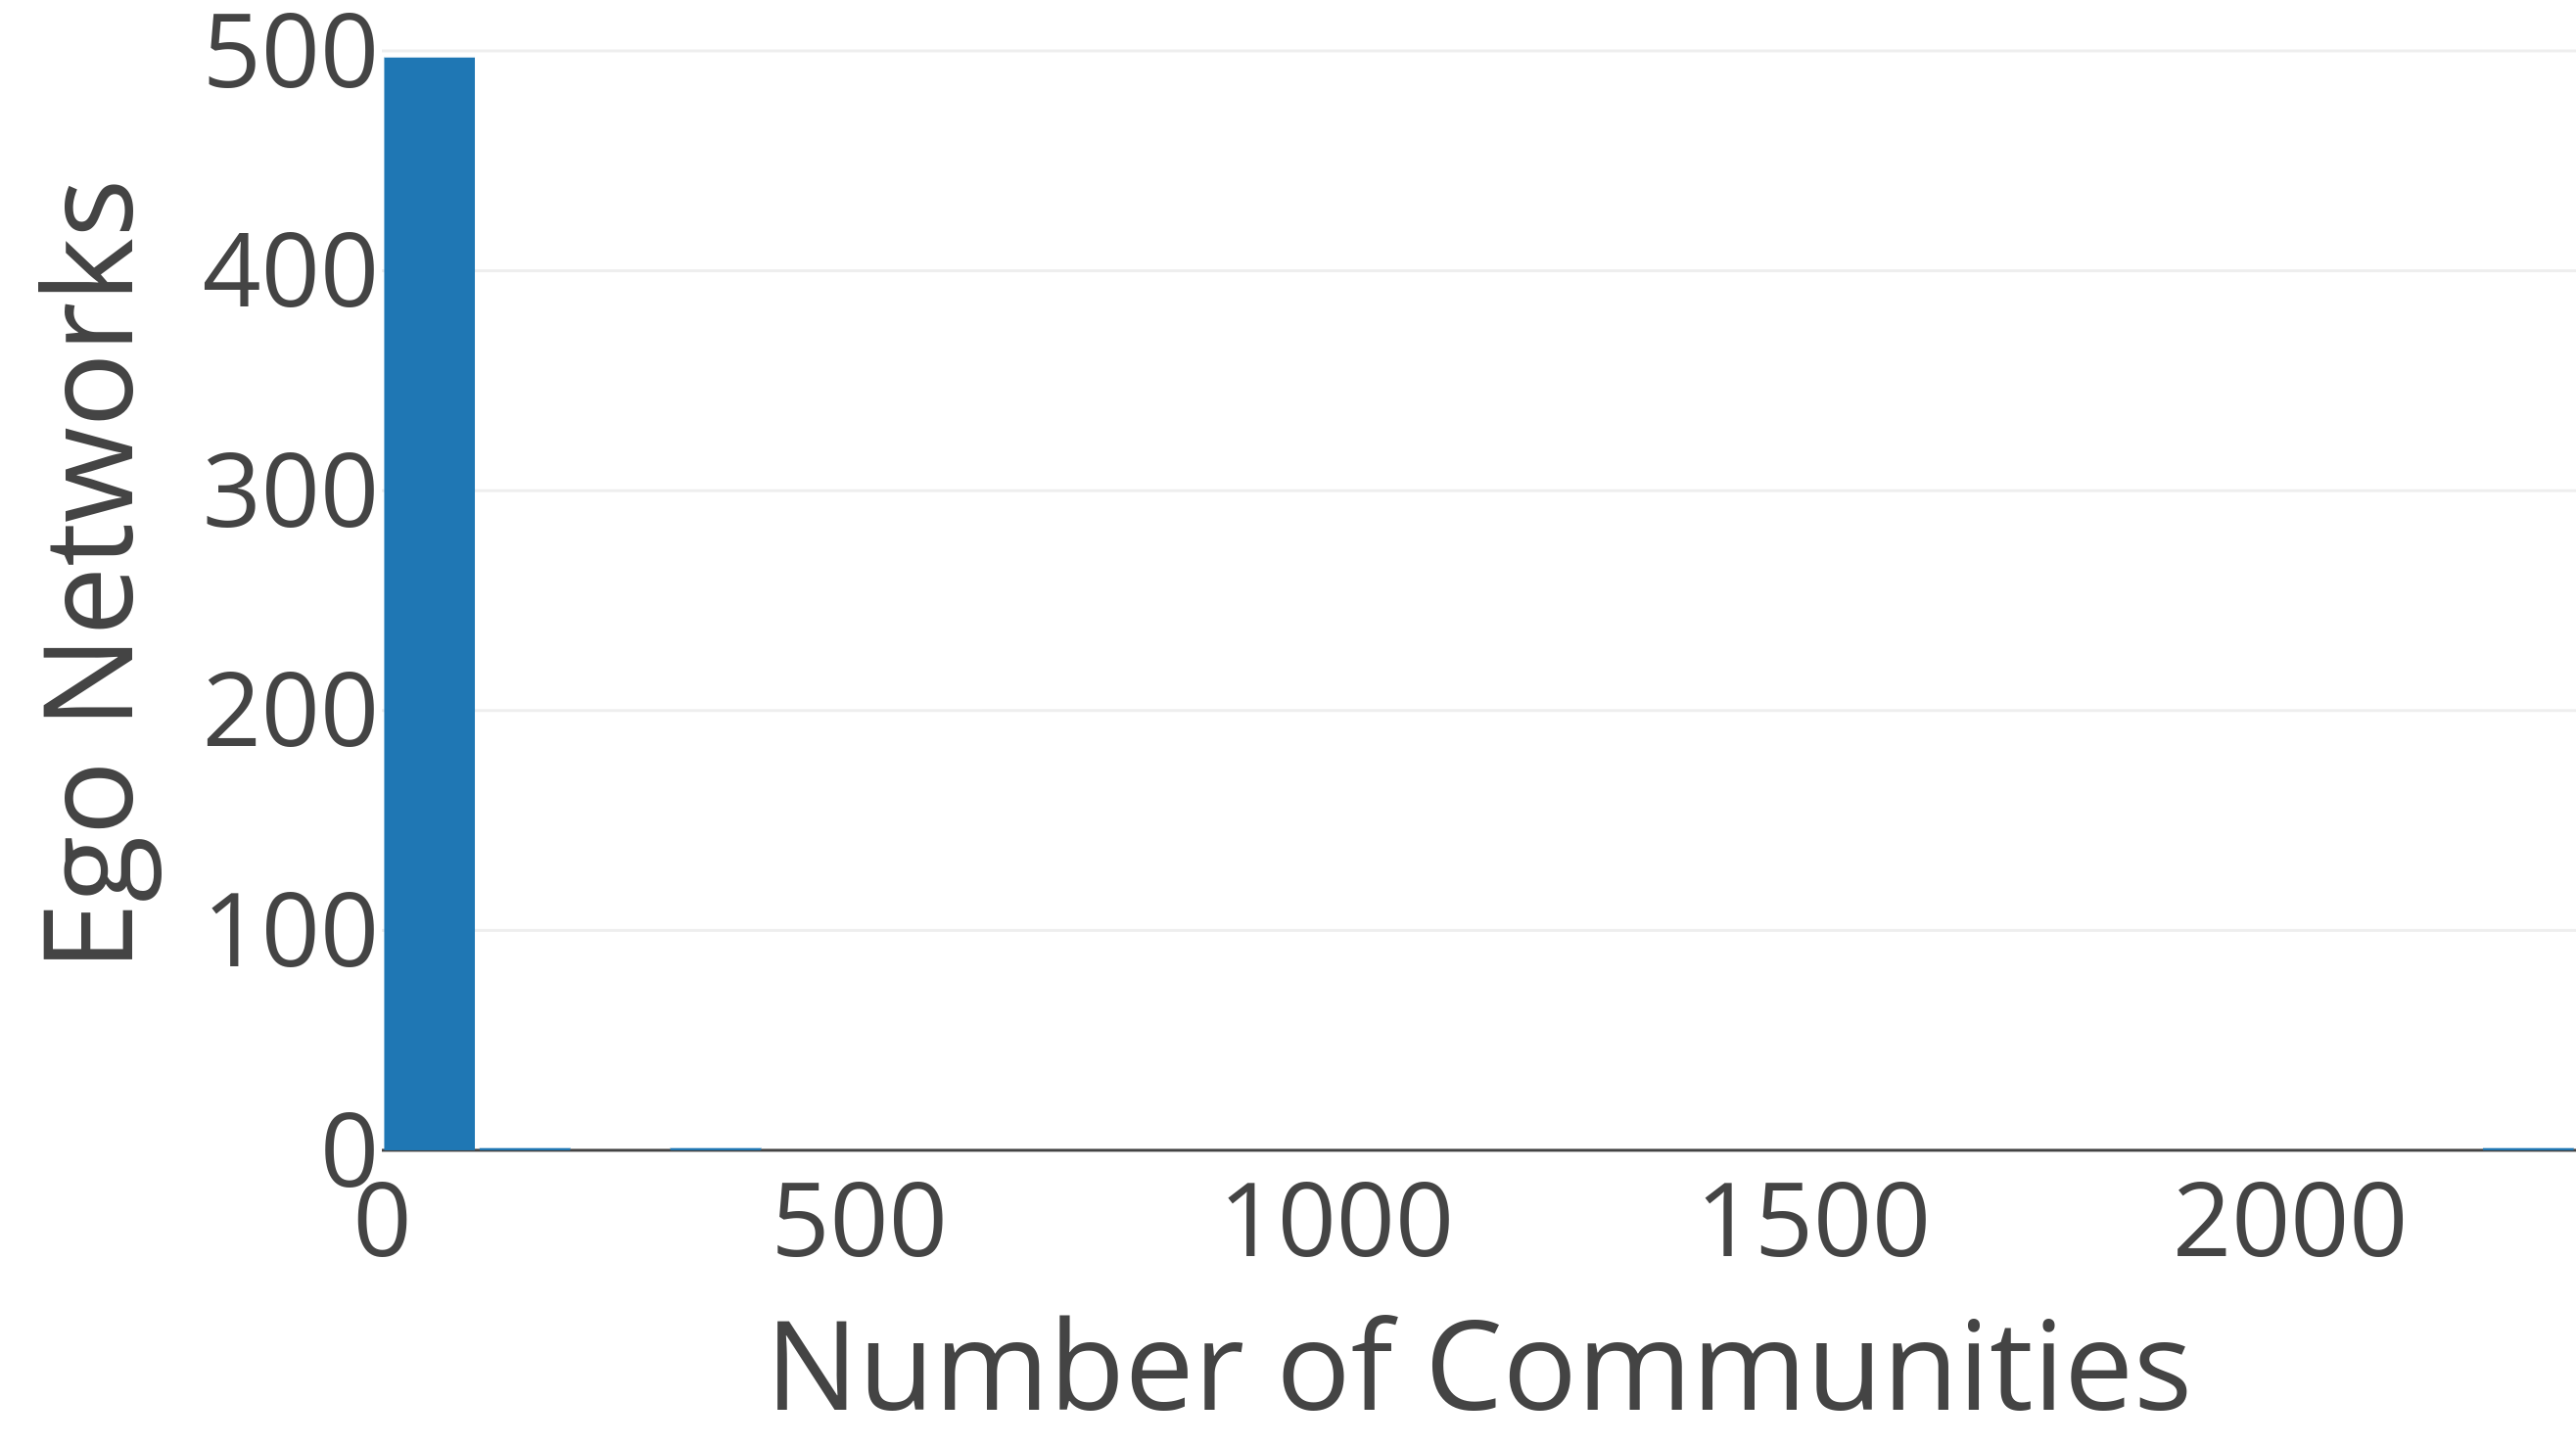
\includegraphics[width=0.47\textwidth]{fig/comm_stats/copra/n_comm/n_comm_copra_follow.png}
        \label{fig:comm_stats_n_comm_copra_follow}
    }
    \subfigure[Retweet]{
        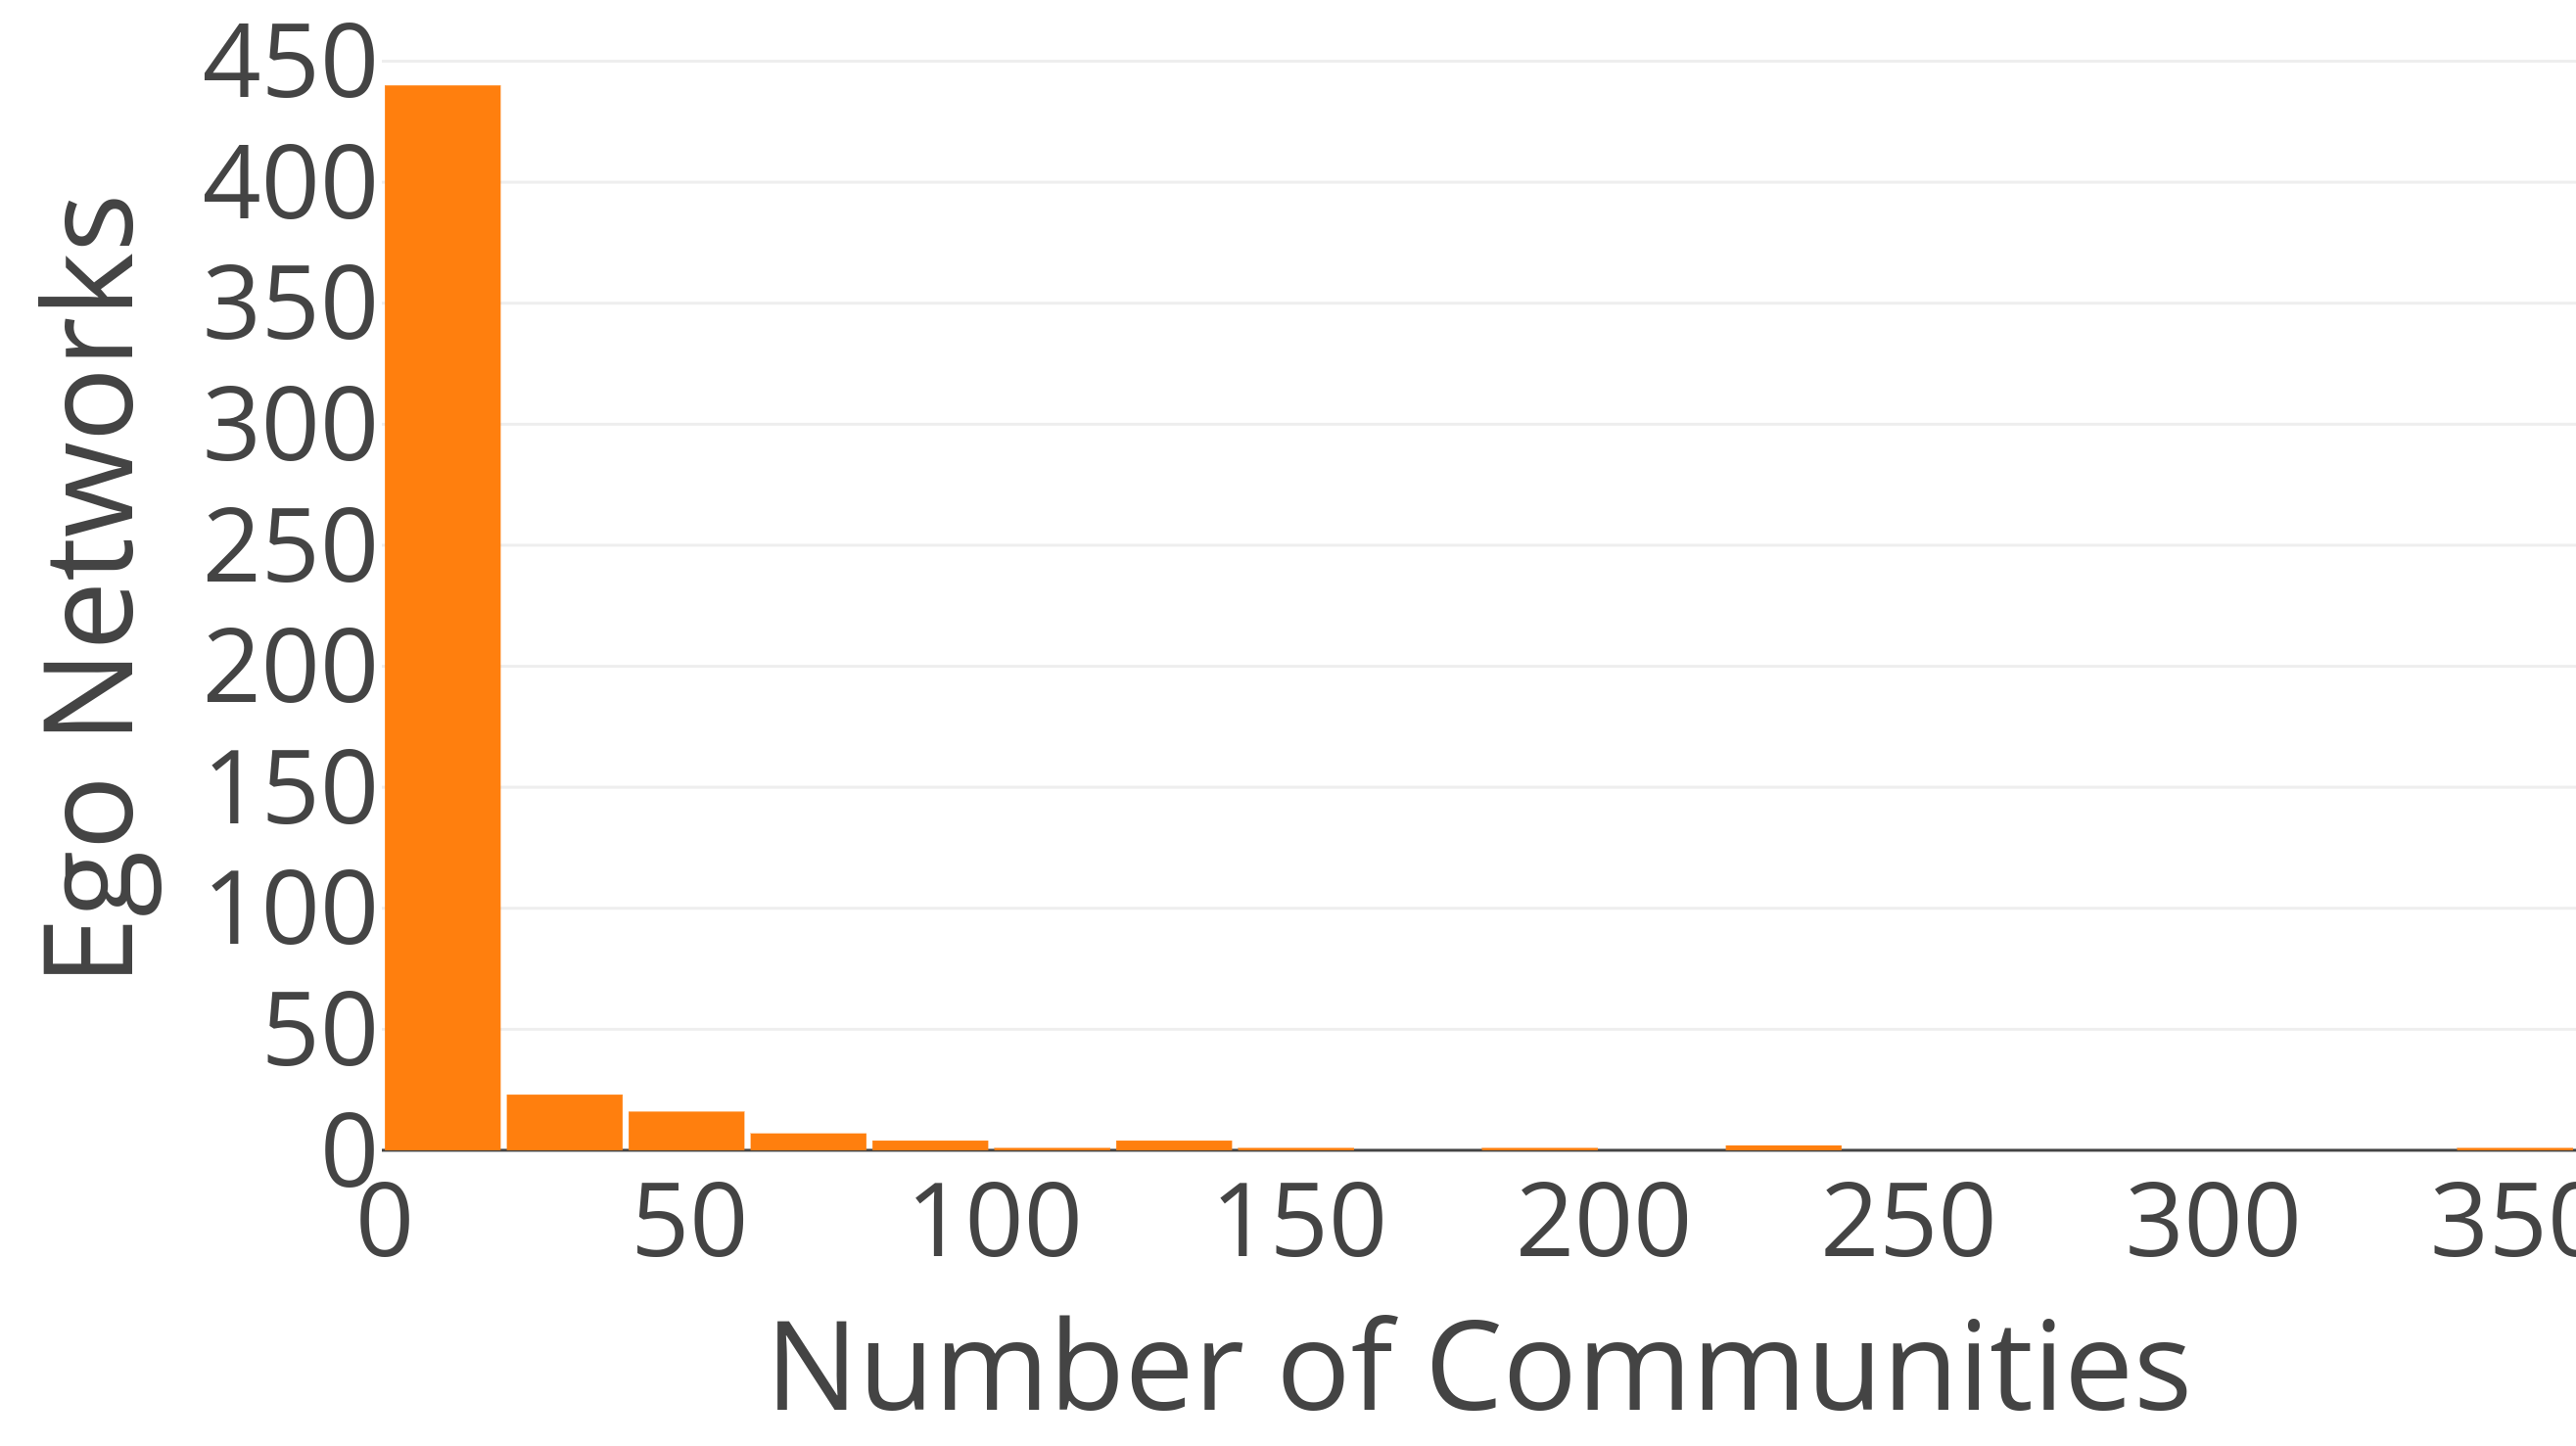
\includegraphics[width=0.47\textwidth]{fig/comm_stats/copra/n_comm/n_comm_copra_retweet.png}
        \label{fig:comm_stats_n_comm_copra_retweet}
    } \\
    \subfigure[Like]{
        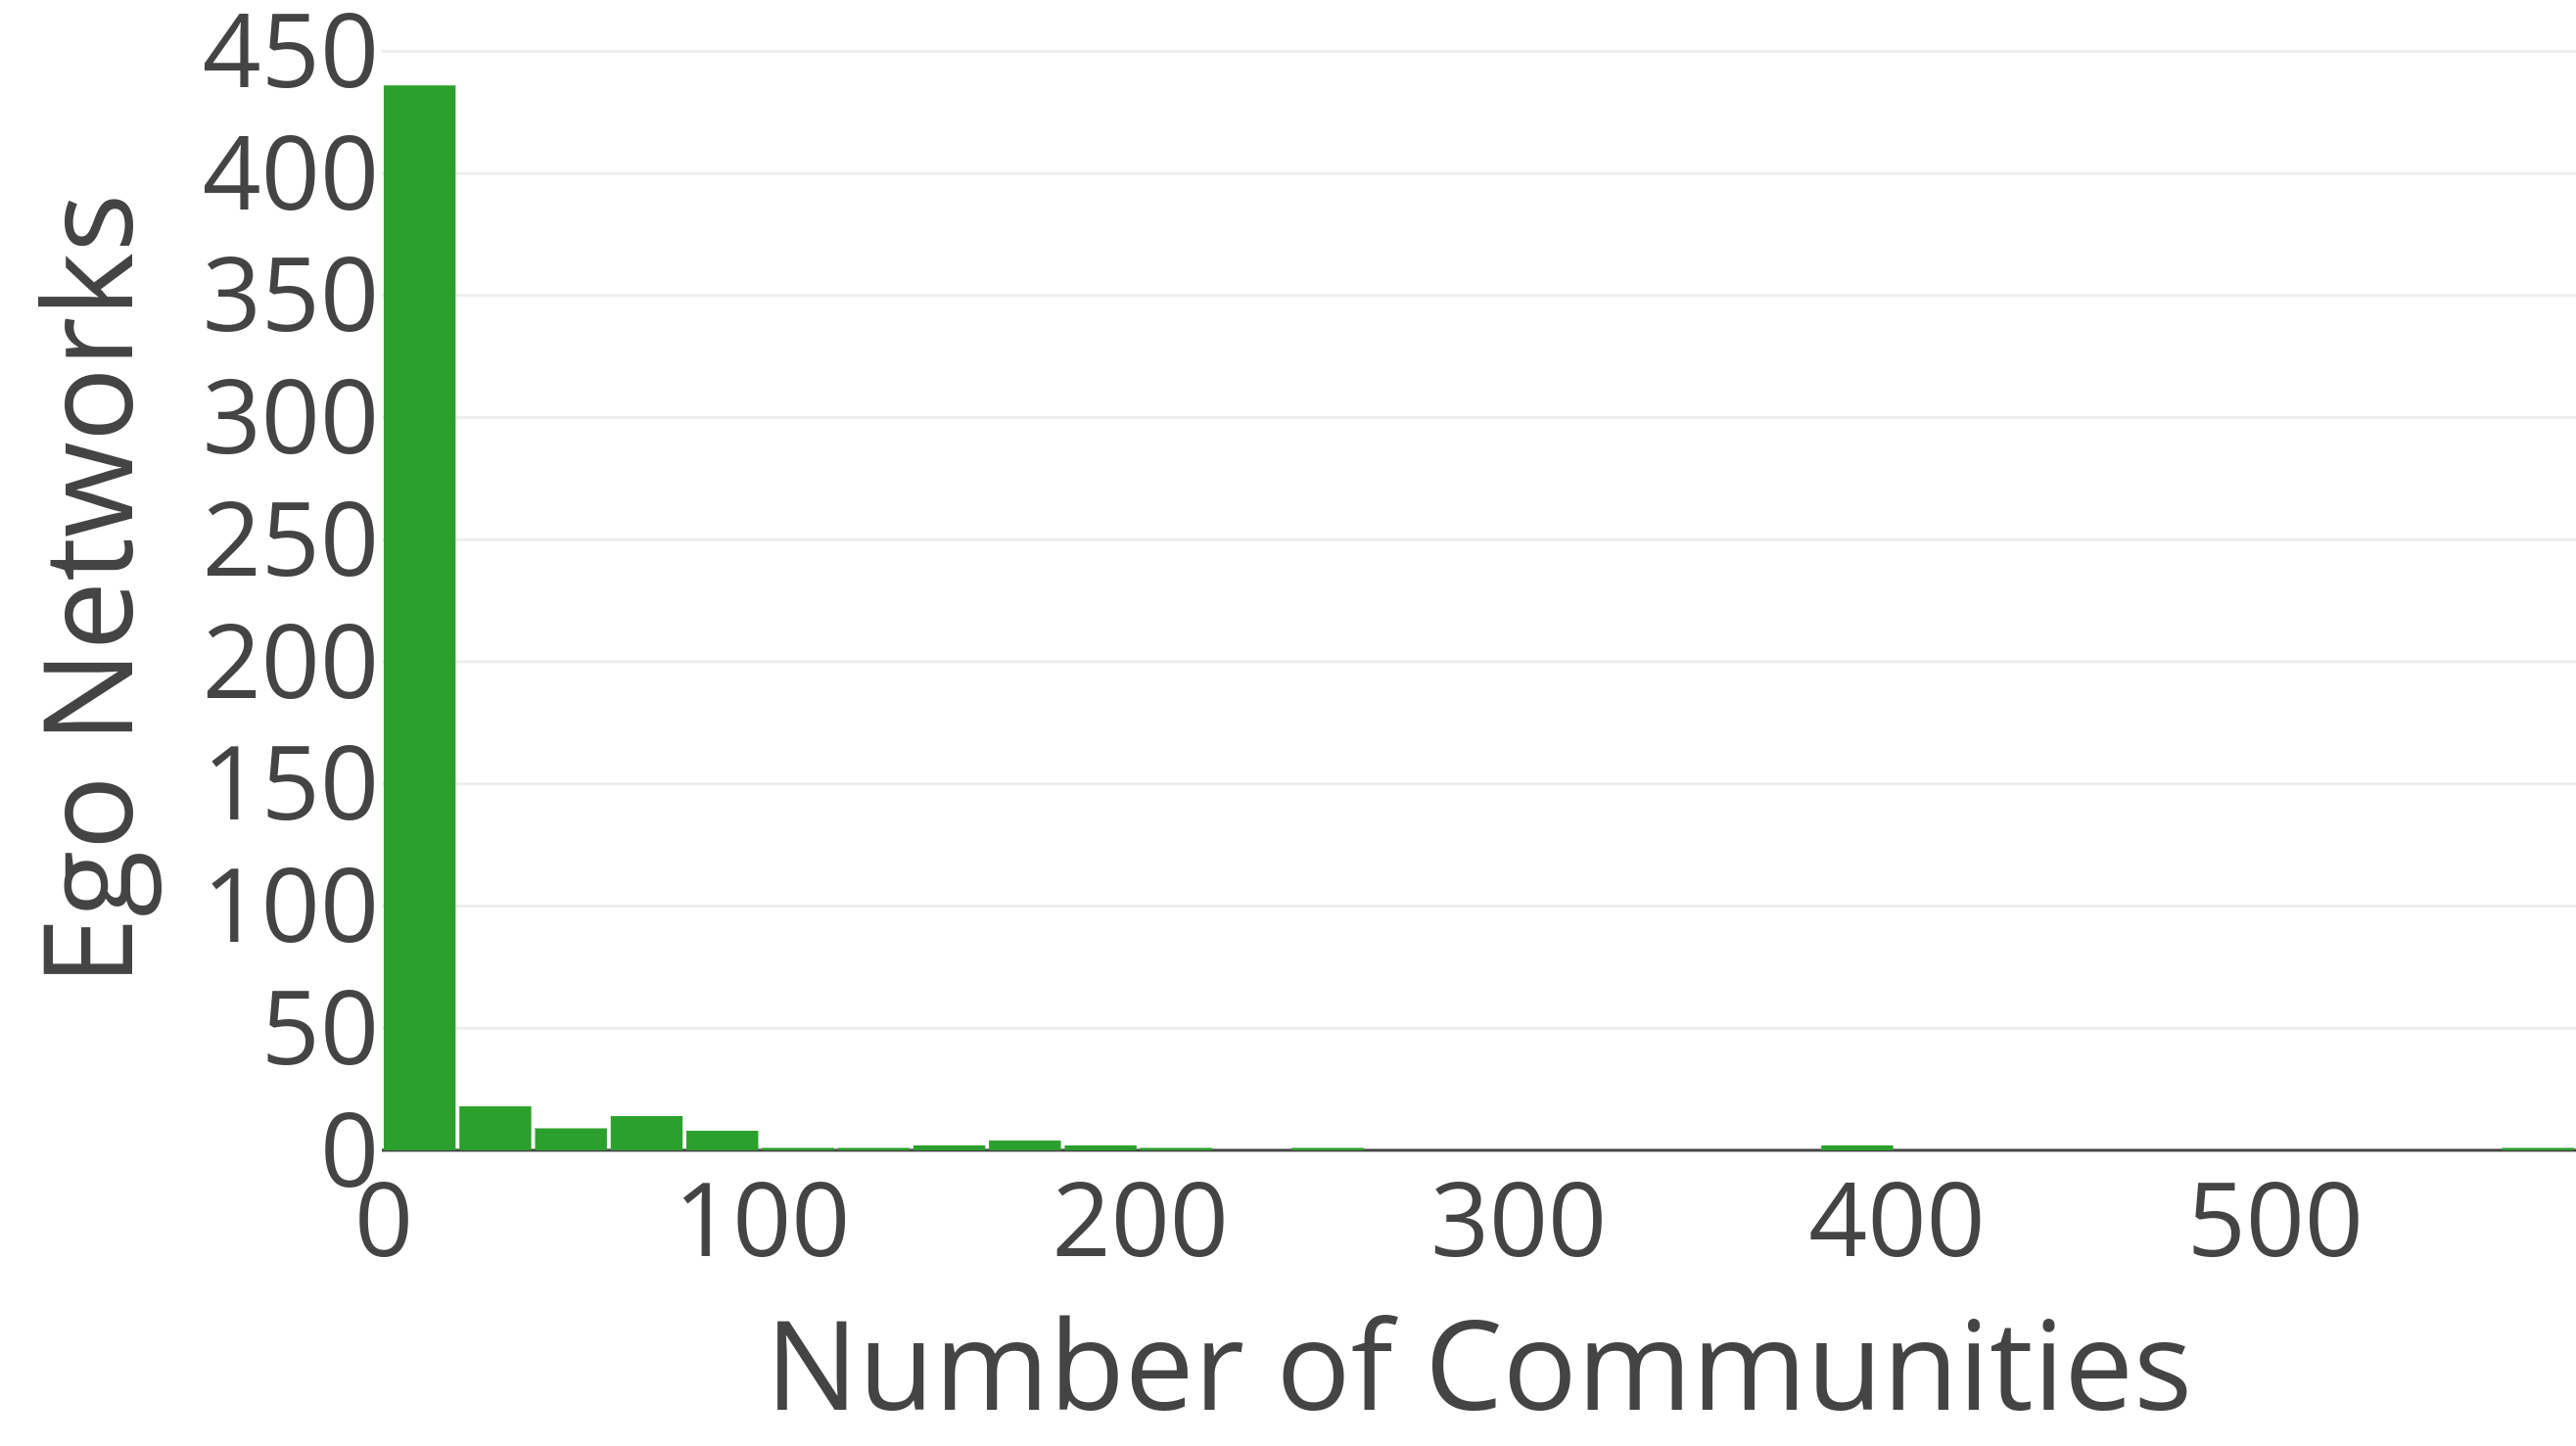
\includegraphics[width=0.47\textwidth]{fig/comm_stats/copra/n_comm/n_comm_copra_like.png}
        \label{fig:comm_stats_n_comm_copra_like}
    }
    \subfigure[Mention]{
        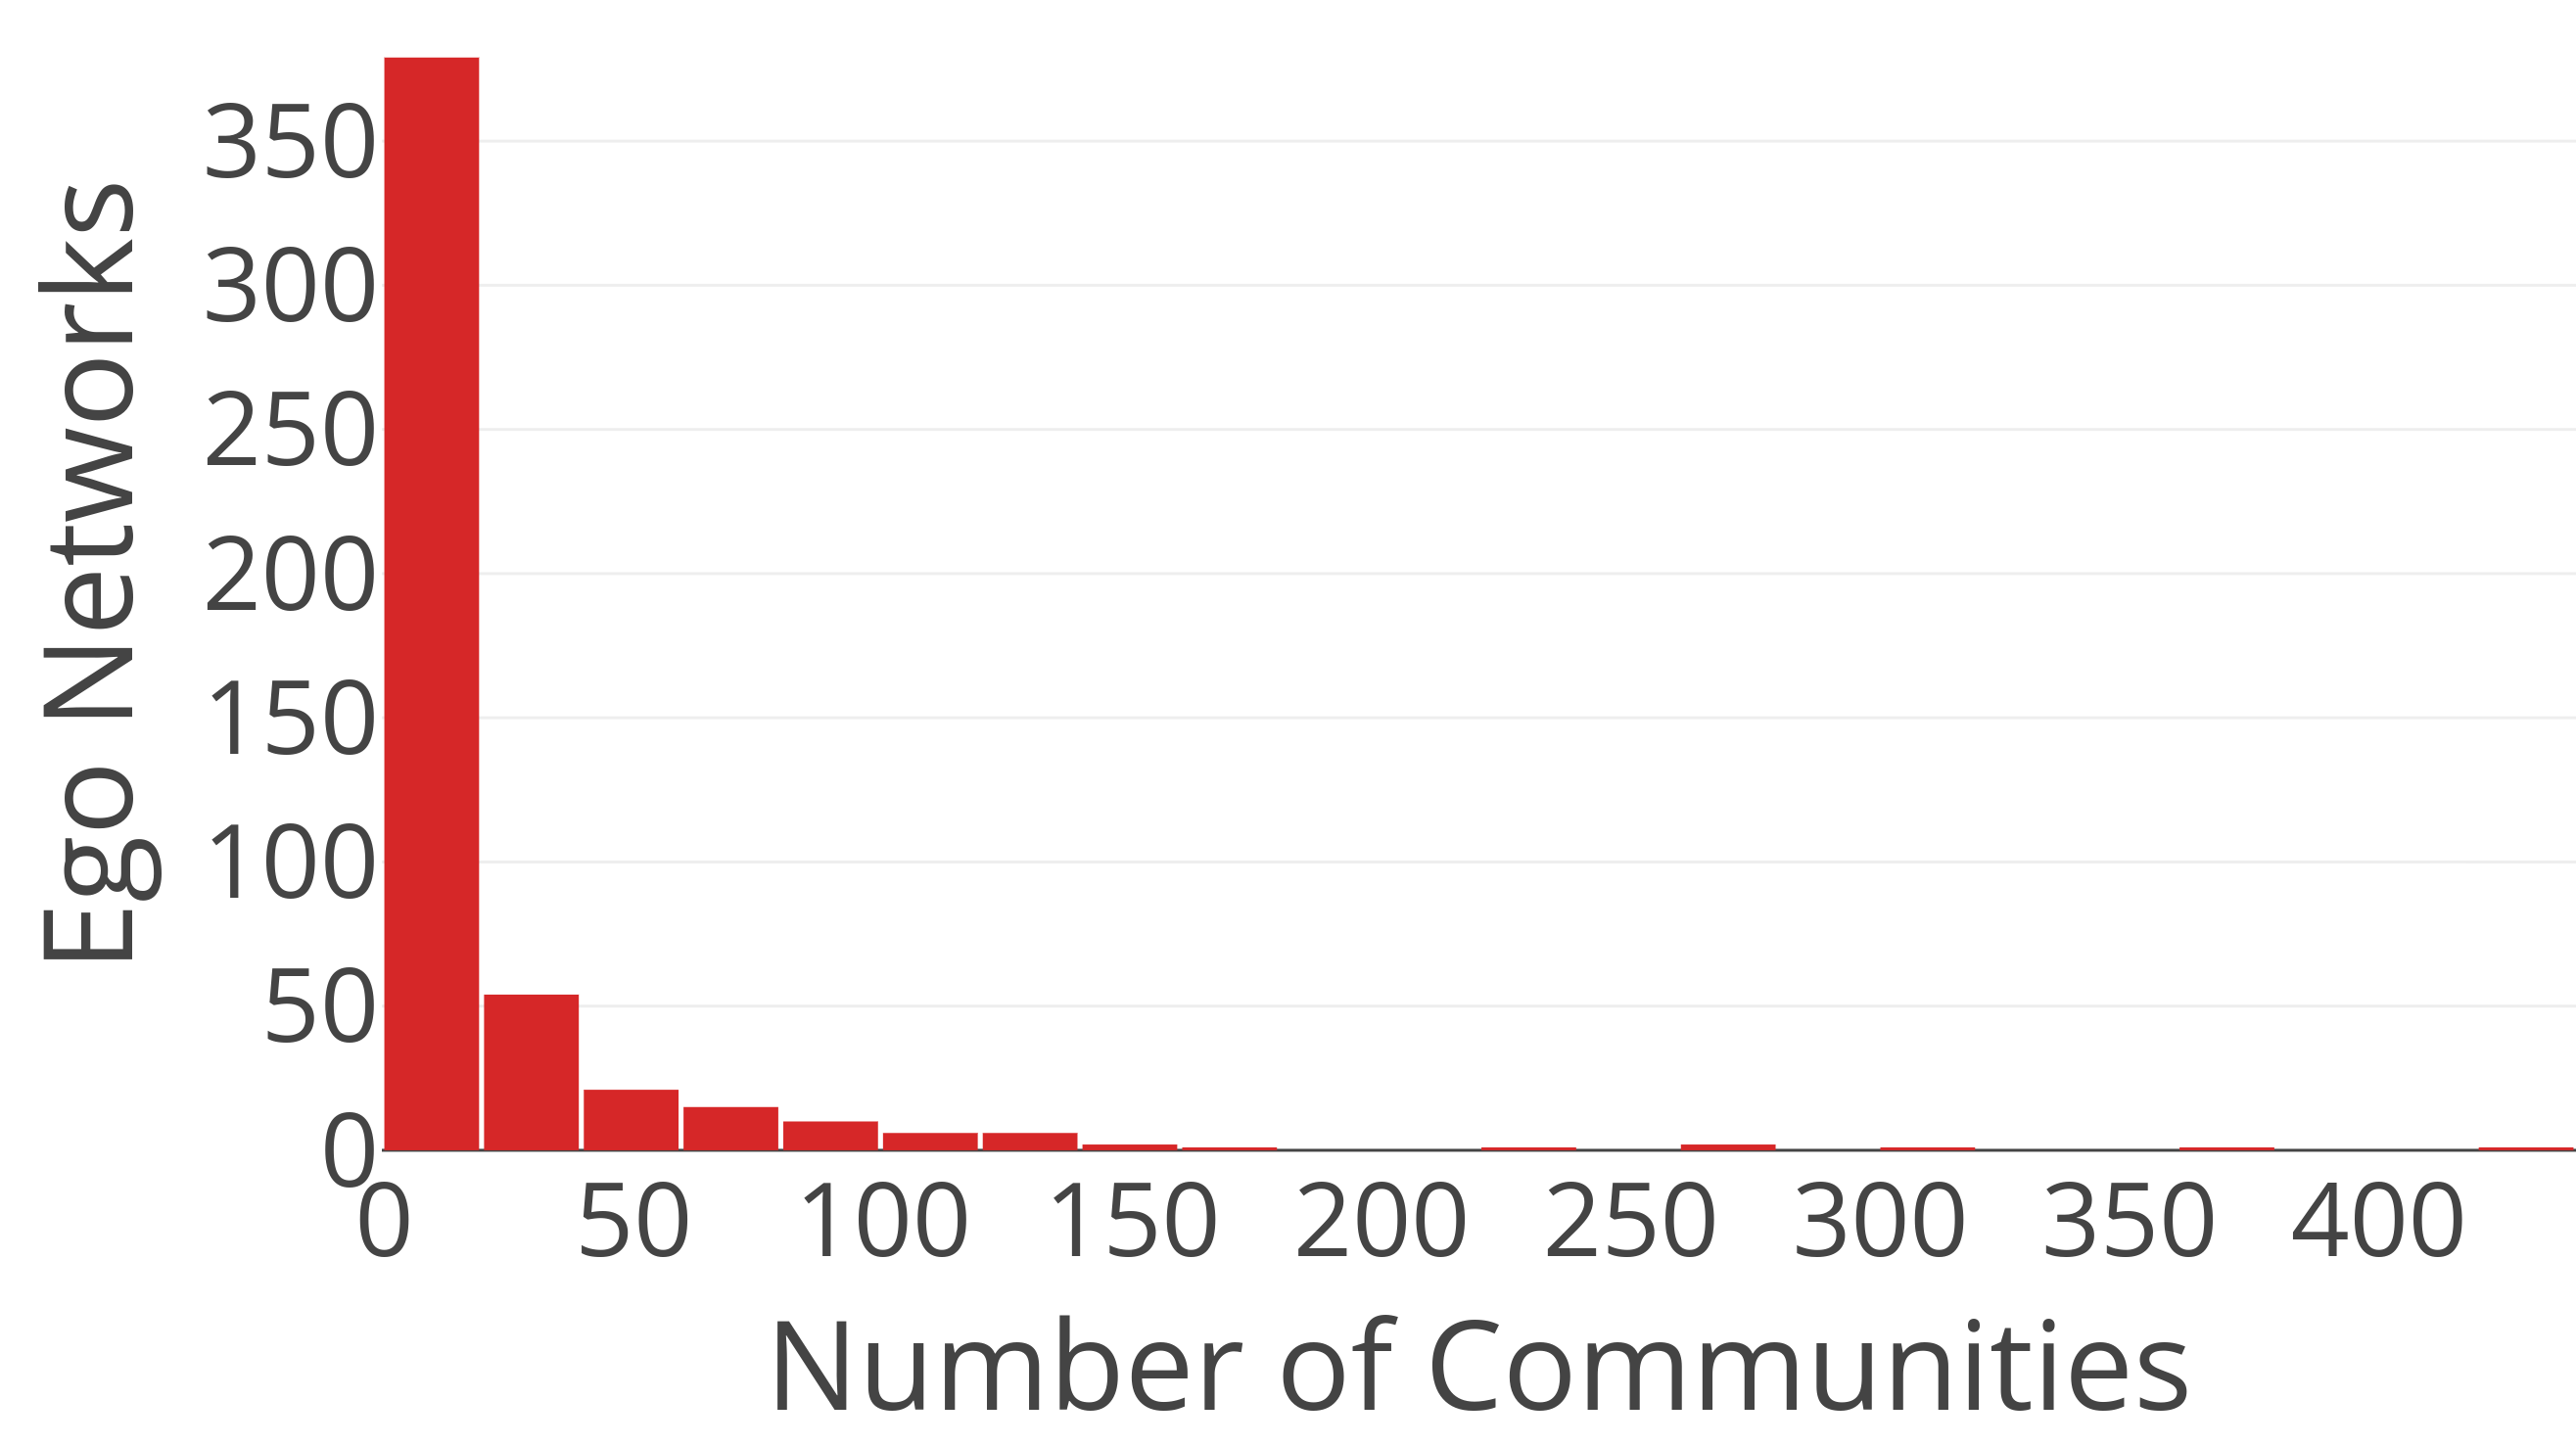
\includegraphics[width=0.47\textwidth]{fig/comm_stats/copra/n_comm/n_comm_copra_mention.png}
        \label{fig:comm_stats_n_comm_copra_mention}
    }
    \caption{Number of communities detected by COPRA.}
    \label{fig:comm_stats_n_comm_copra}
\end{figure}
\begin{figure}[h!tb]
    \centering
    \subfigure[Follow]{
        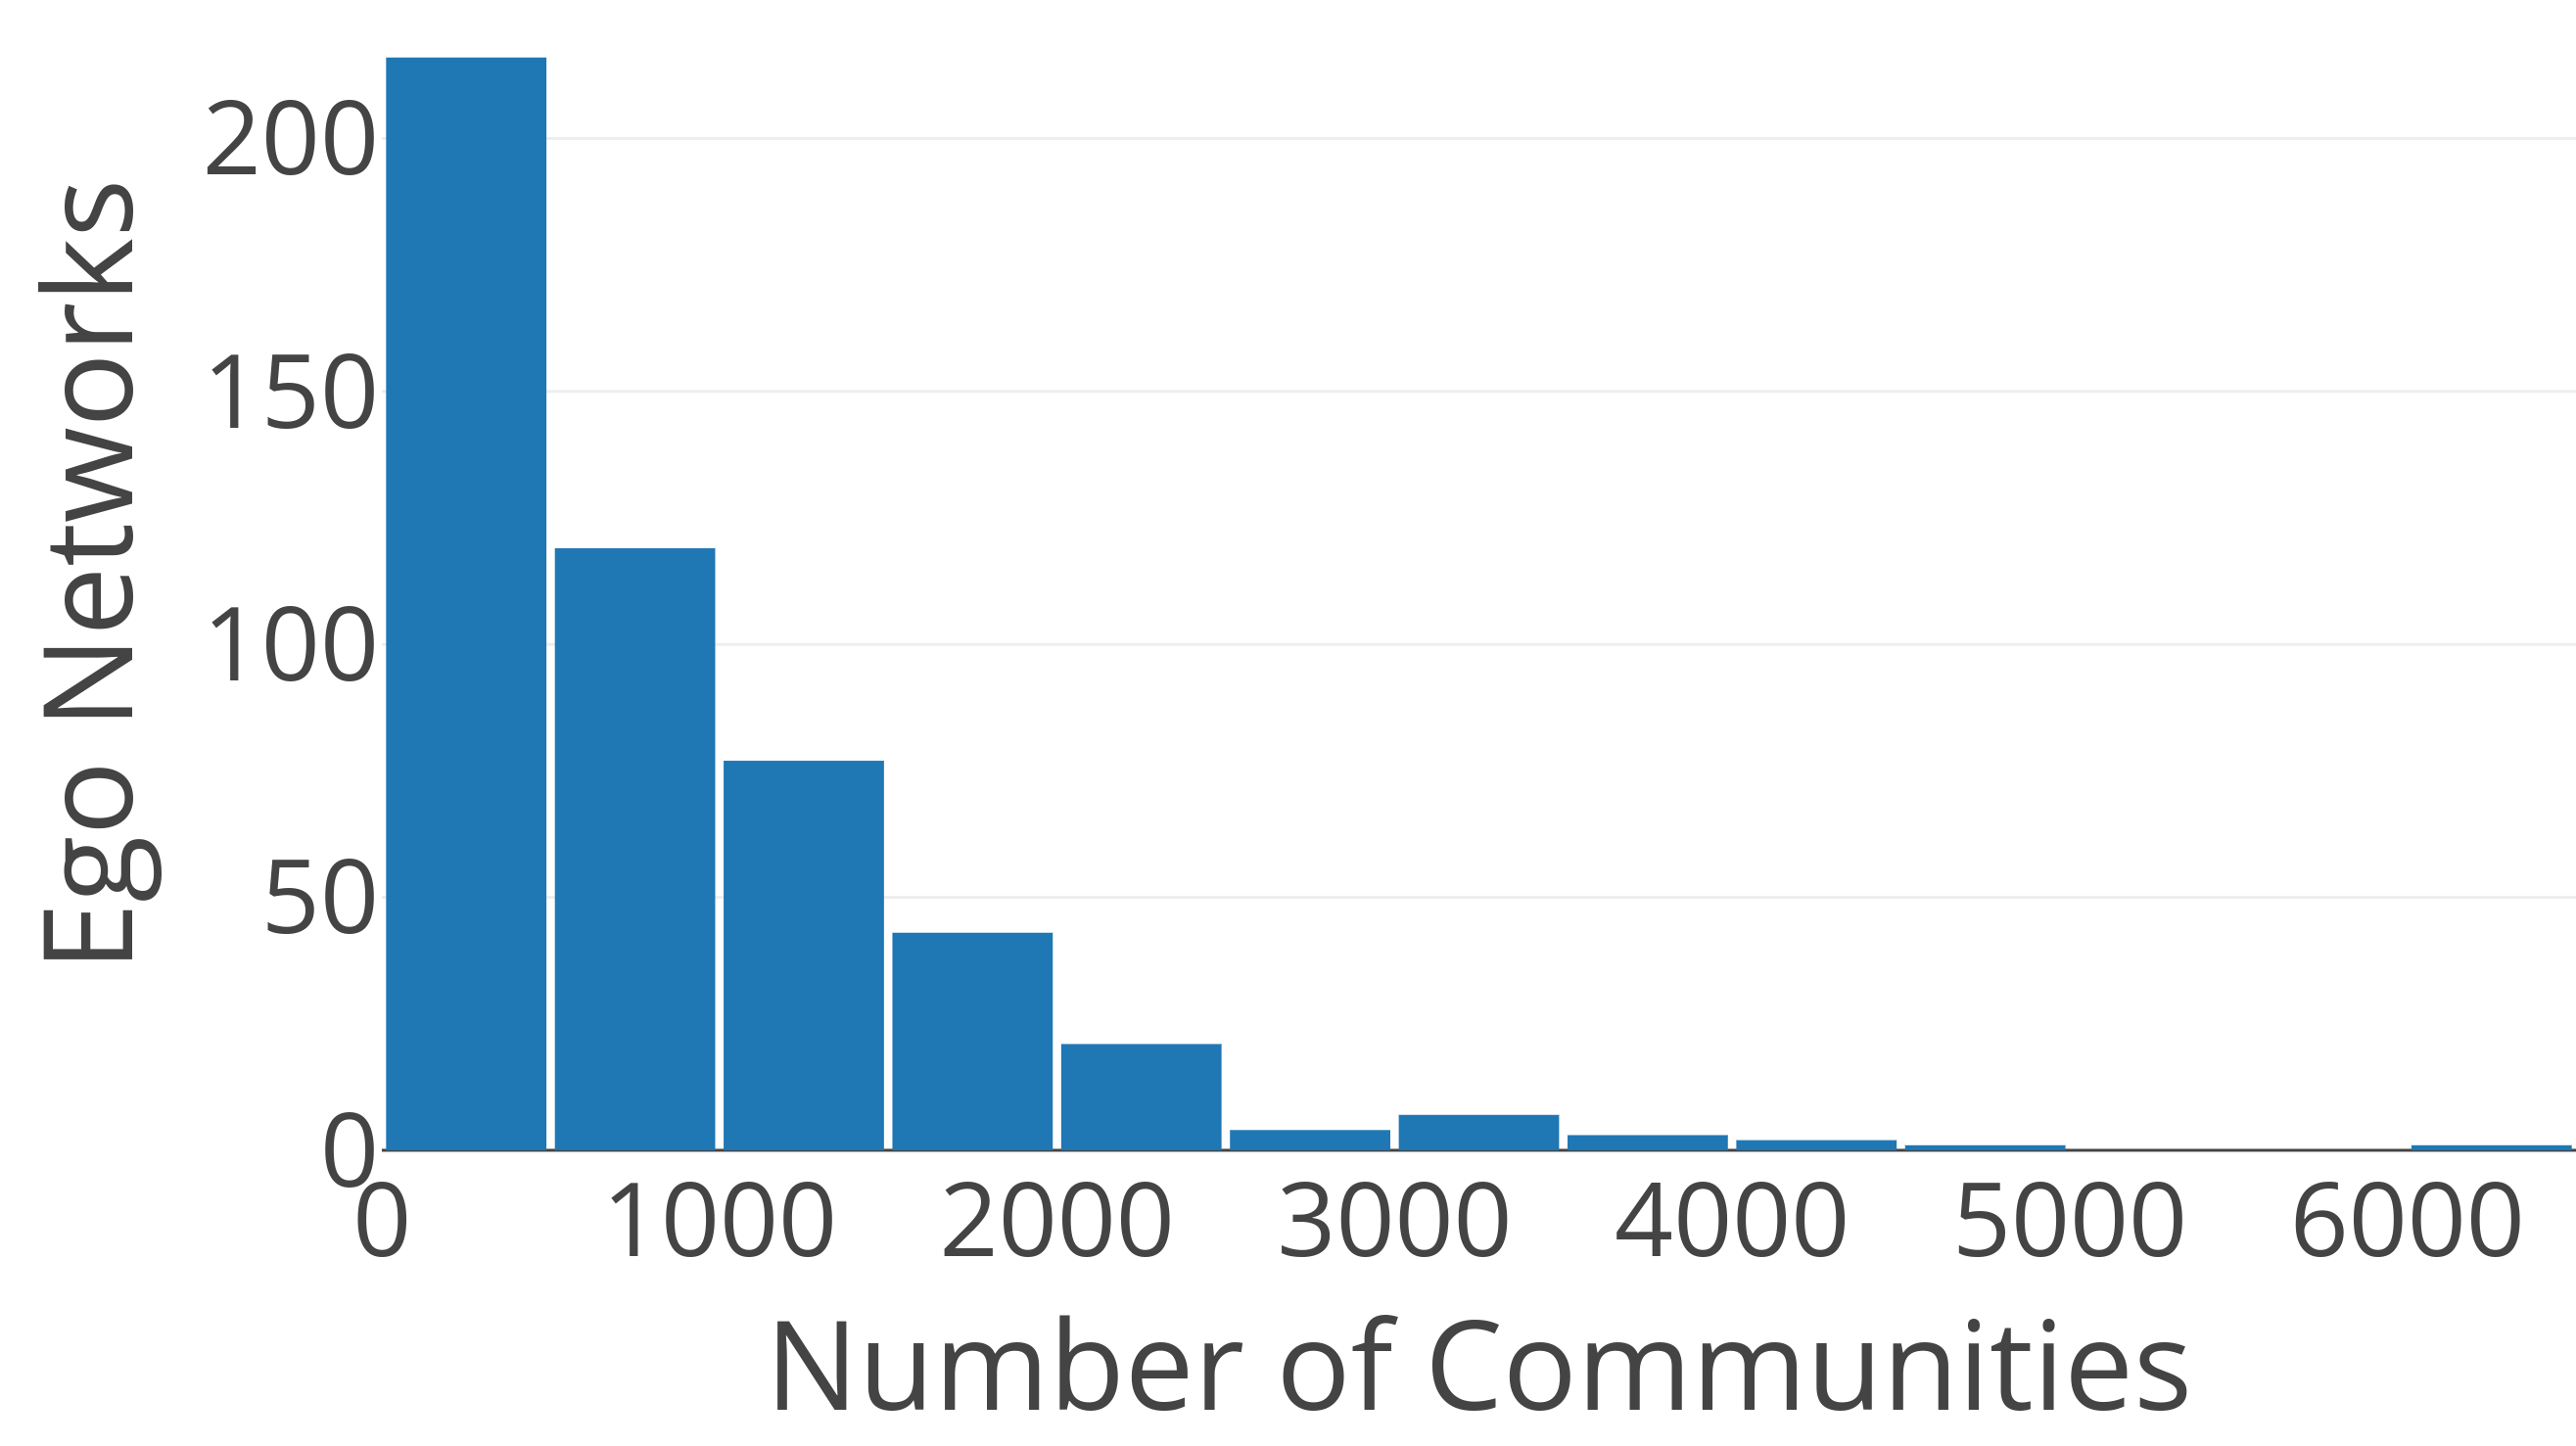
\includegraphics[width=0.47\textwidth]{fig/comm_stats/oslom/n_comm/n_comm_oslom_follow.png}
        \label{fig:comm_stats_n_comm_oslom_follow}
    }
    \subfigure[Retweet]{
        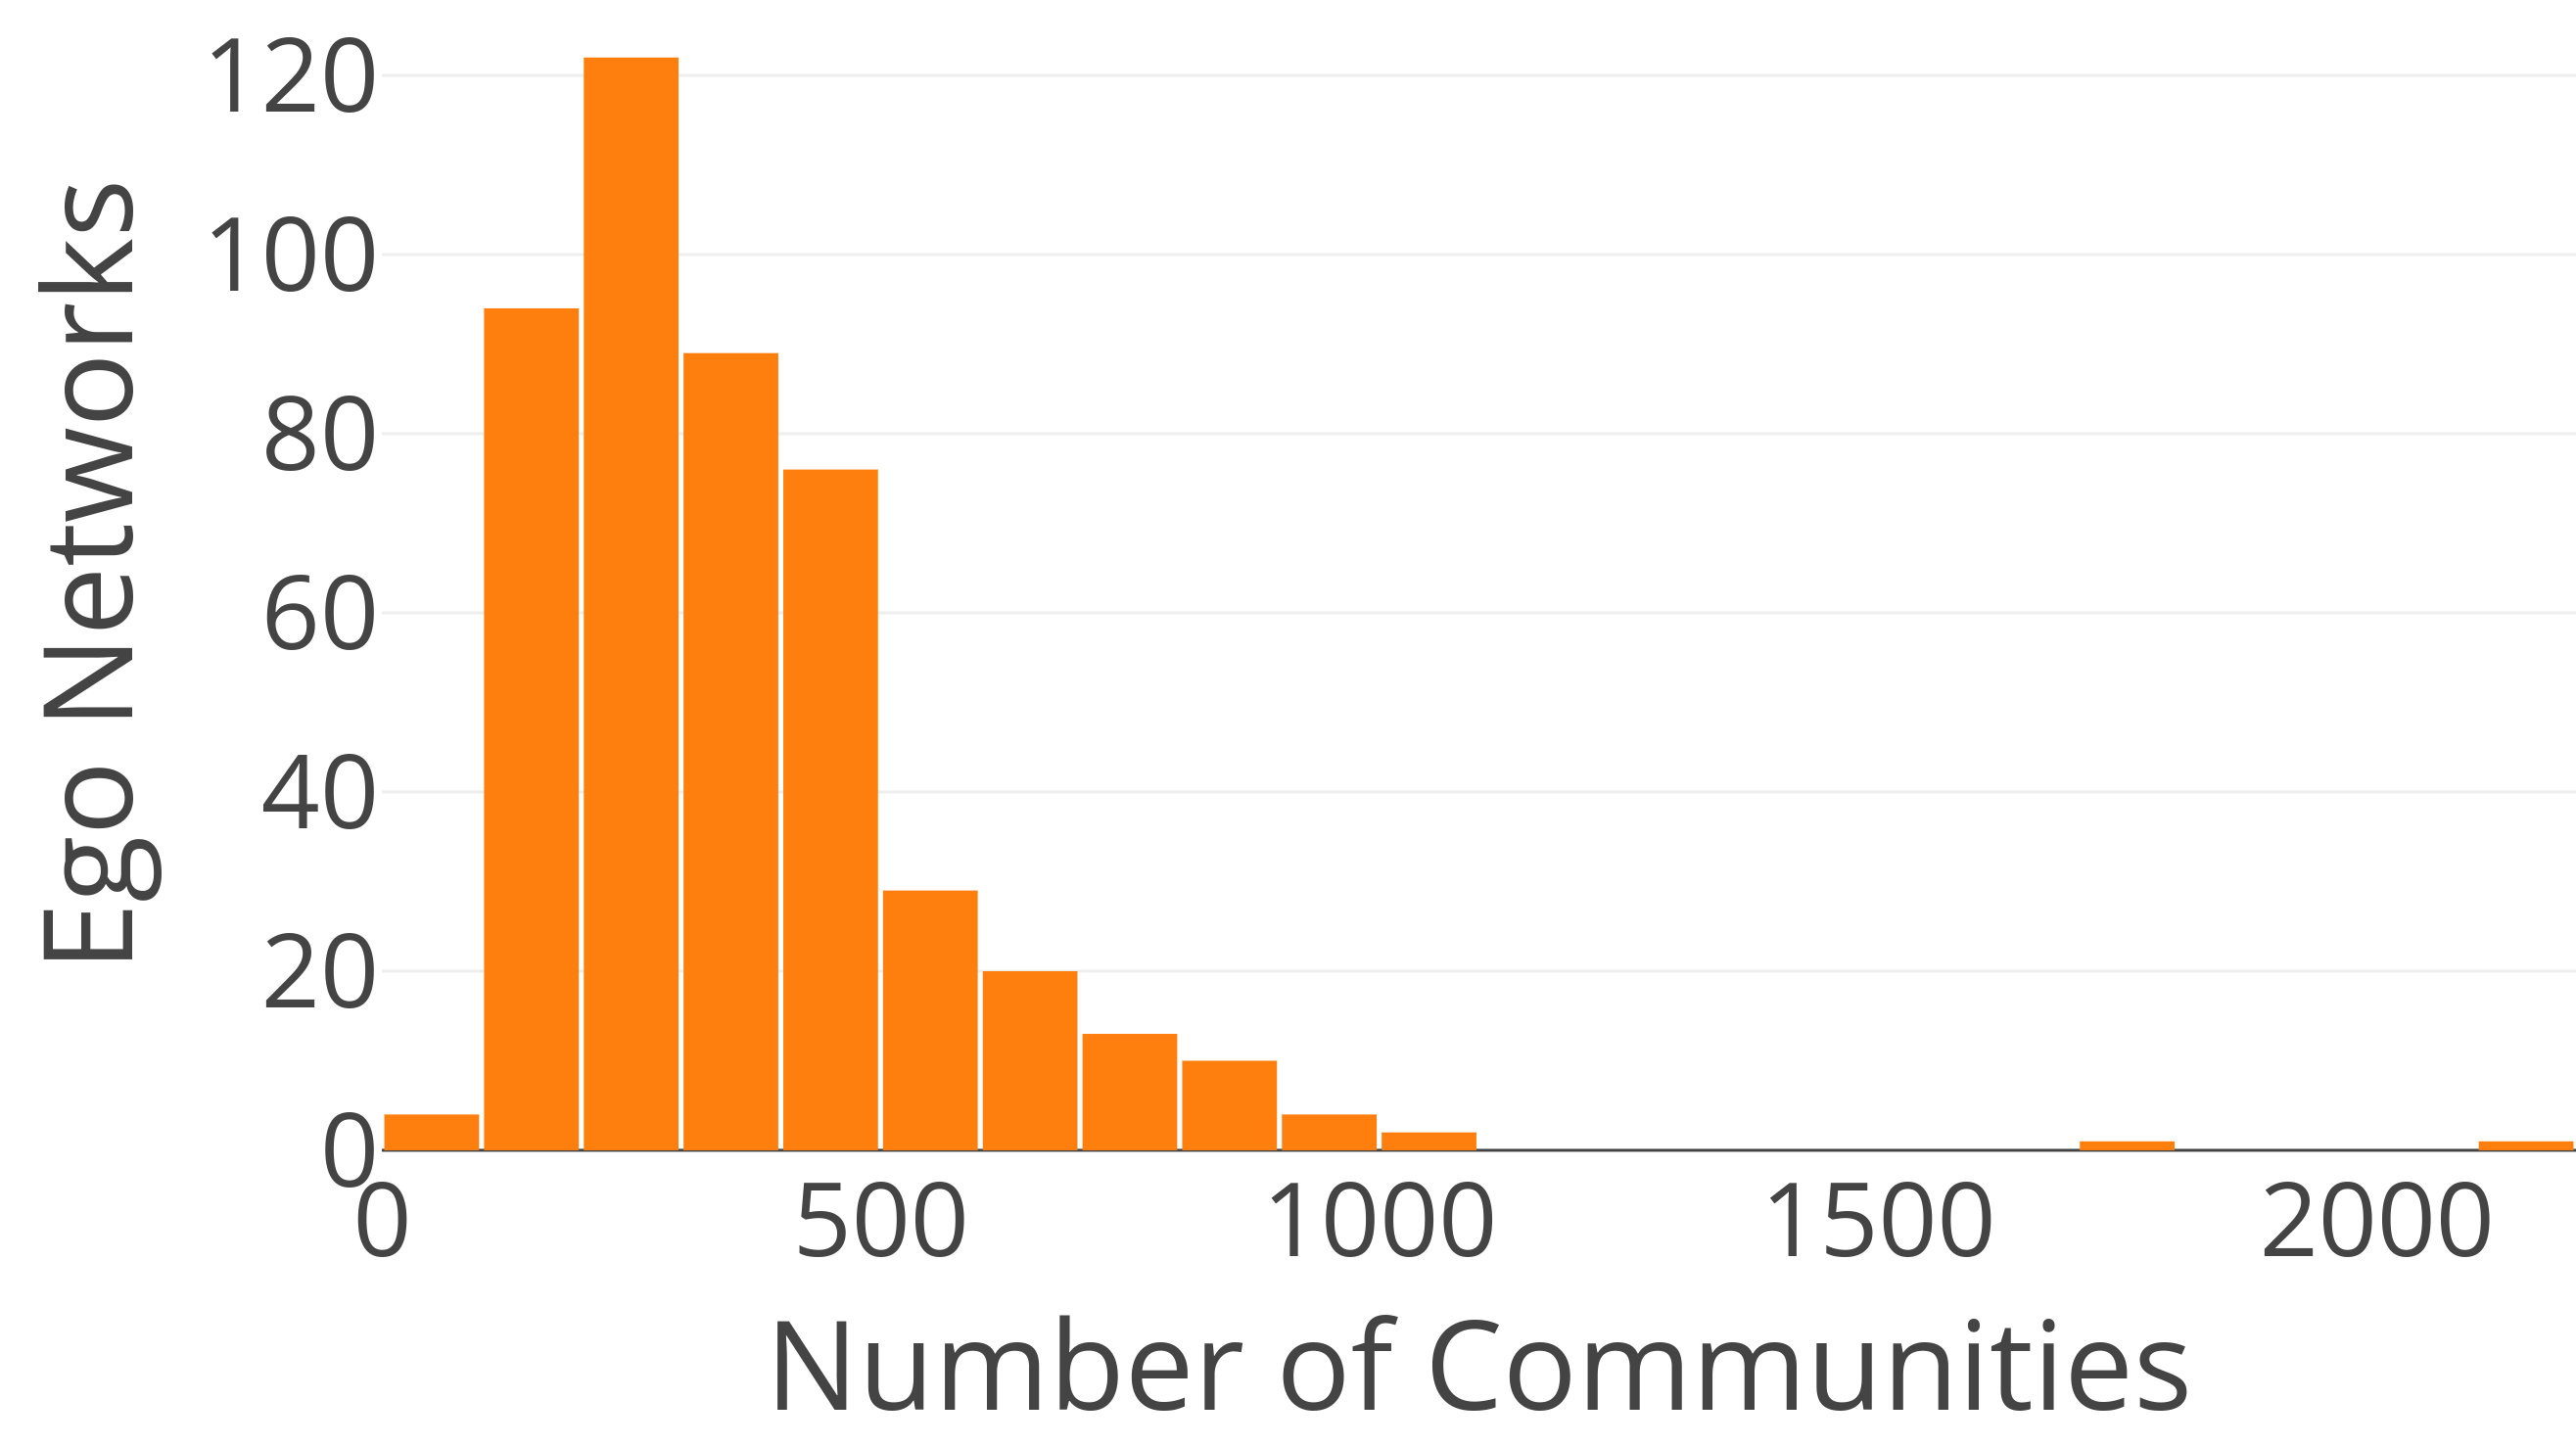
\includegraphics[width=0.47\textwidth]{fig/comm_stats/oslom/n_comm/n_comm_oslom_retweet.png}
        \label{fig:comm_stats_n_comm_oslom_retweet}
    } \\
    \subfigure[Like]{
        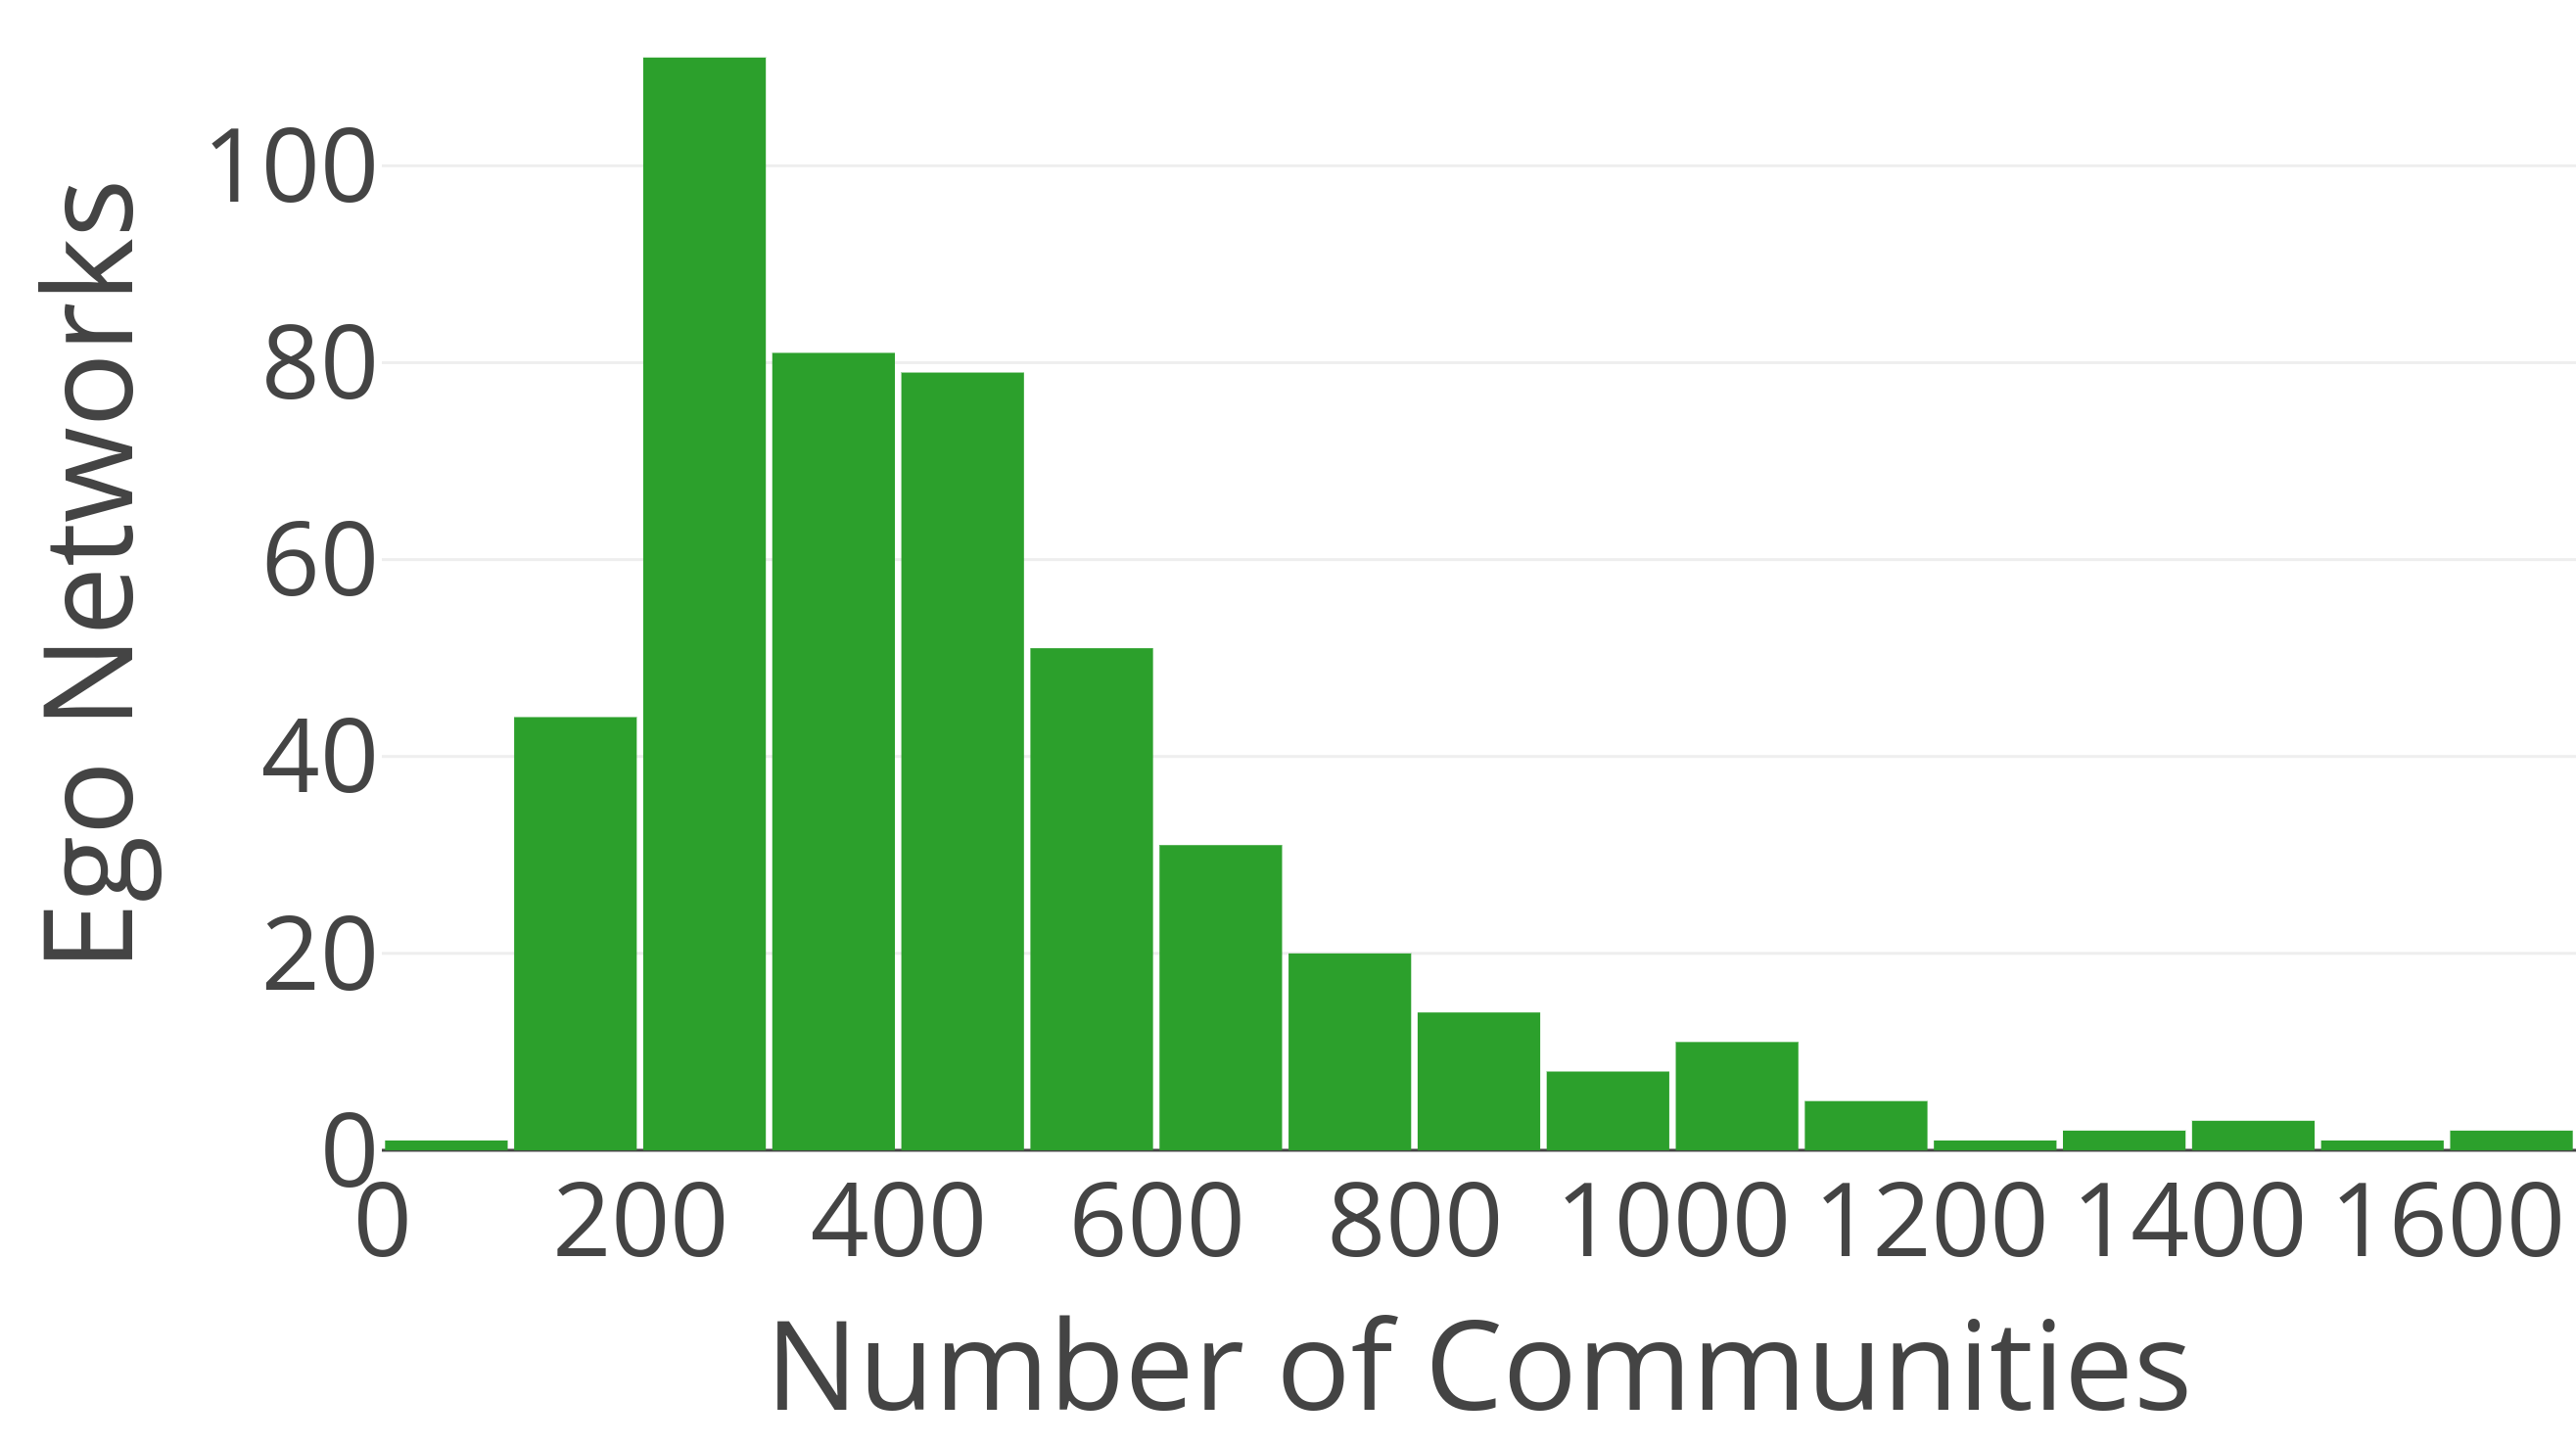
\includegraphics[width=0.47\textwidth]{fig/comm_stats/oslom/n_comm/n_comm_oslom_like.png}
        \label{fig:comm_stats_n_comm_oslom_like}
    }
    \subfigure[Mention]{
        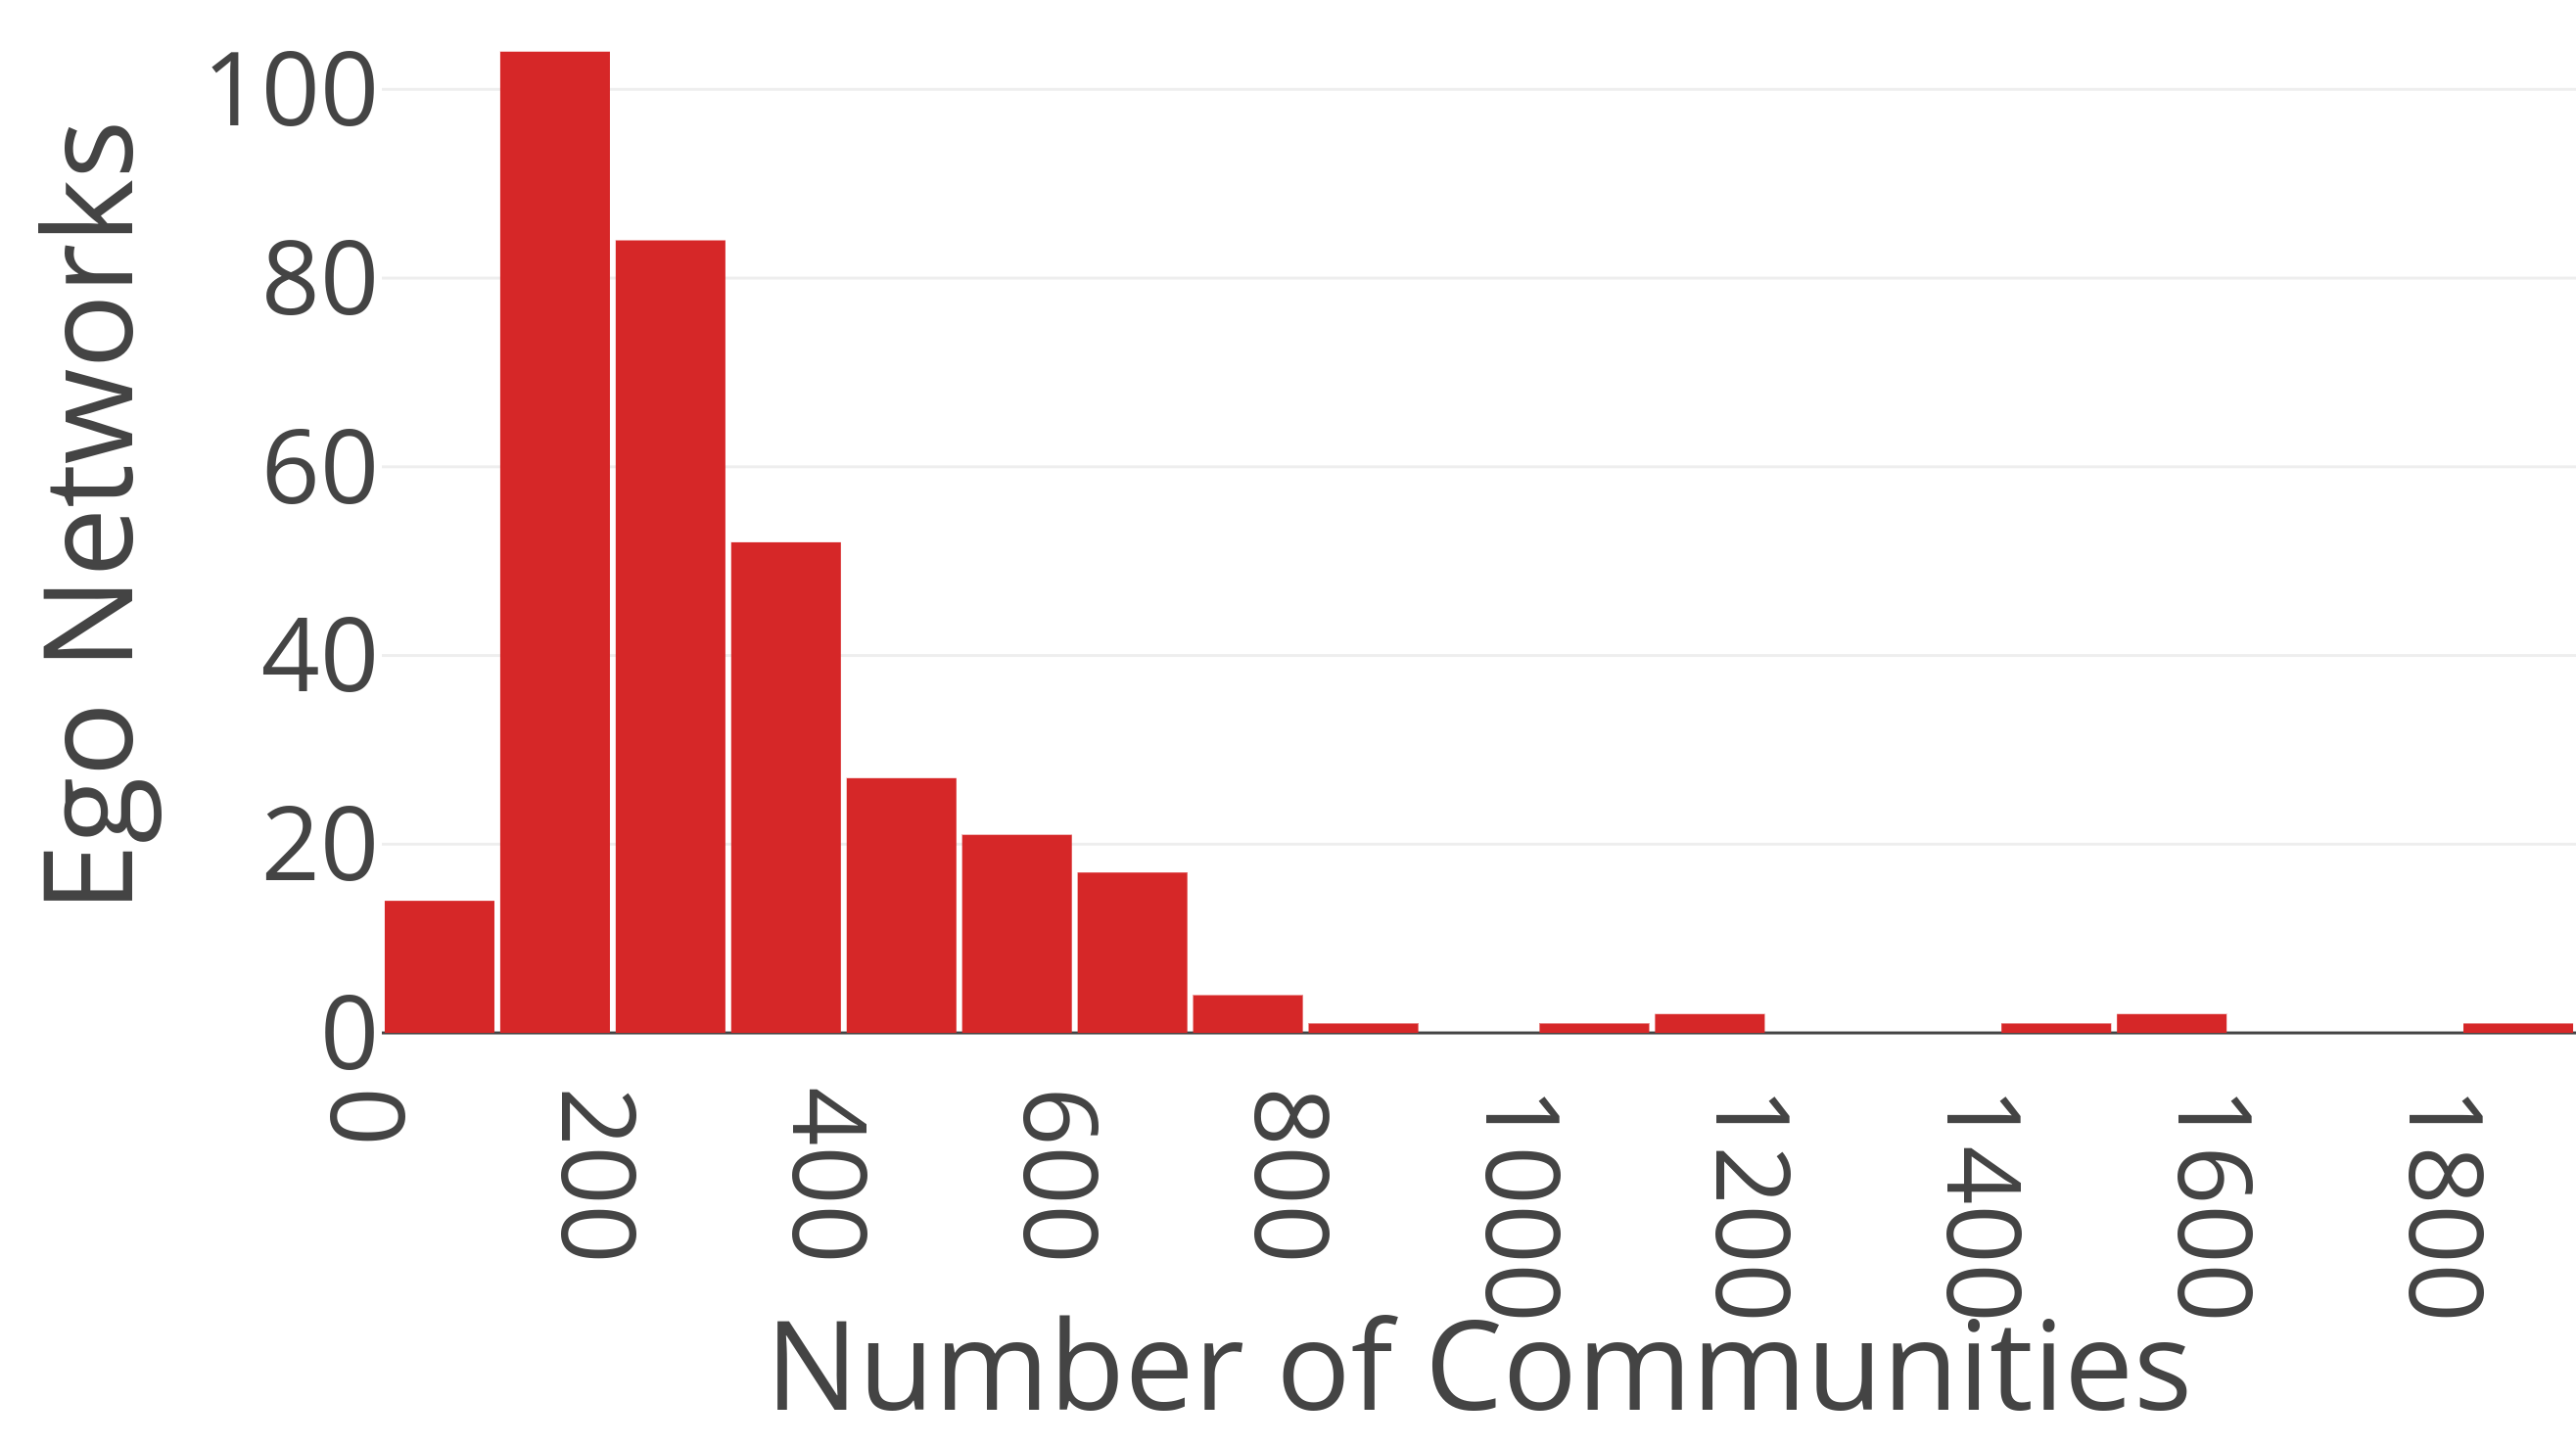
\includegraphics[width=0.47\textwidth]{fig/comm_stats/oslom/n_comm/n_comm_oslom_mention.png}
        \label{fig:comm_stats_n_comm_oslom_mention}
    }
    \caption{Number of communities detected by OSLOM.}
    \label{fig:comm_stats_n_comm_oslom}
\end{figure}

We compute the number of communities detected by each algorithm in each of the layers of all ego networks. The results are presented in figures \ref{fig:comm_stats_n_comm_rak}, \ref{fig:comm_stats_n_comm_infomap}, \ref{fig:comm_stats_n_comm_copra} and \ref{fig:comm_stats_n_comm_oslom} through histograms with the frequency distribution of the detected communities. The results indicate that the vertices of all the layers of the analyzed ego networks have similar behavior. For the algorithms INFOMAP and OSLOM, the vertices tend to form communities, and for the RAK and COPRA algorithms the networks themselves, or at least most of the vertices of the ego network, are considered as a single community.

The Fig. \ref{fig:comm_stats_n_comm_rak} shows a histogram with the frequency distribution of the number of communities detected by the algorithm RAK. For most egos networks this algorithm detected few communities at all layers, while few ego networks exhibit a high number of communities. Fig. \ref{fig:comm_stats_n_comm_infomap} shows a histogram for the number of communities detected by the INFOMAP algorithm. Unlike RAK, INFOMAP detects a greater number of communities for all layers. Fig. \ref{fig:comm_stats_n_comm_copra} shows a plot with the number of communities detected by the COPRA algorithm, and the results are very similar to those found with the RAK algorithm. Fig. \ref{fig:comm_stats_n_comm_oslom} shows the number of communities detected with the OSLOM algorithm, which is the algorithm that can identify the largest number of communities, but it is worth remembering that the COPRA and OSLOM algorithms detect overlap, that is to say that a vertex can be associated with more than one community.

%However, INFOMAP presented the best average values for most community evaluation measures considered in Section \ref{sec:comm_quality}, thus we report only INFOMAP results  in this work. We have that the sizes of the communities vary greatly inside a layer for a given ego. In the great majority of the cases the mean size of the communities is  much smaller than the standard deviation. In most cases the biggest community is much greater than the mean sizes and the smallest contains only one alter. 

\begin{figure}[h!tb]
    \centering
    \subfigure[RAK]{
        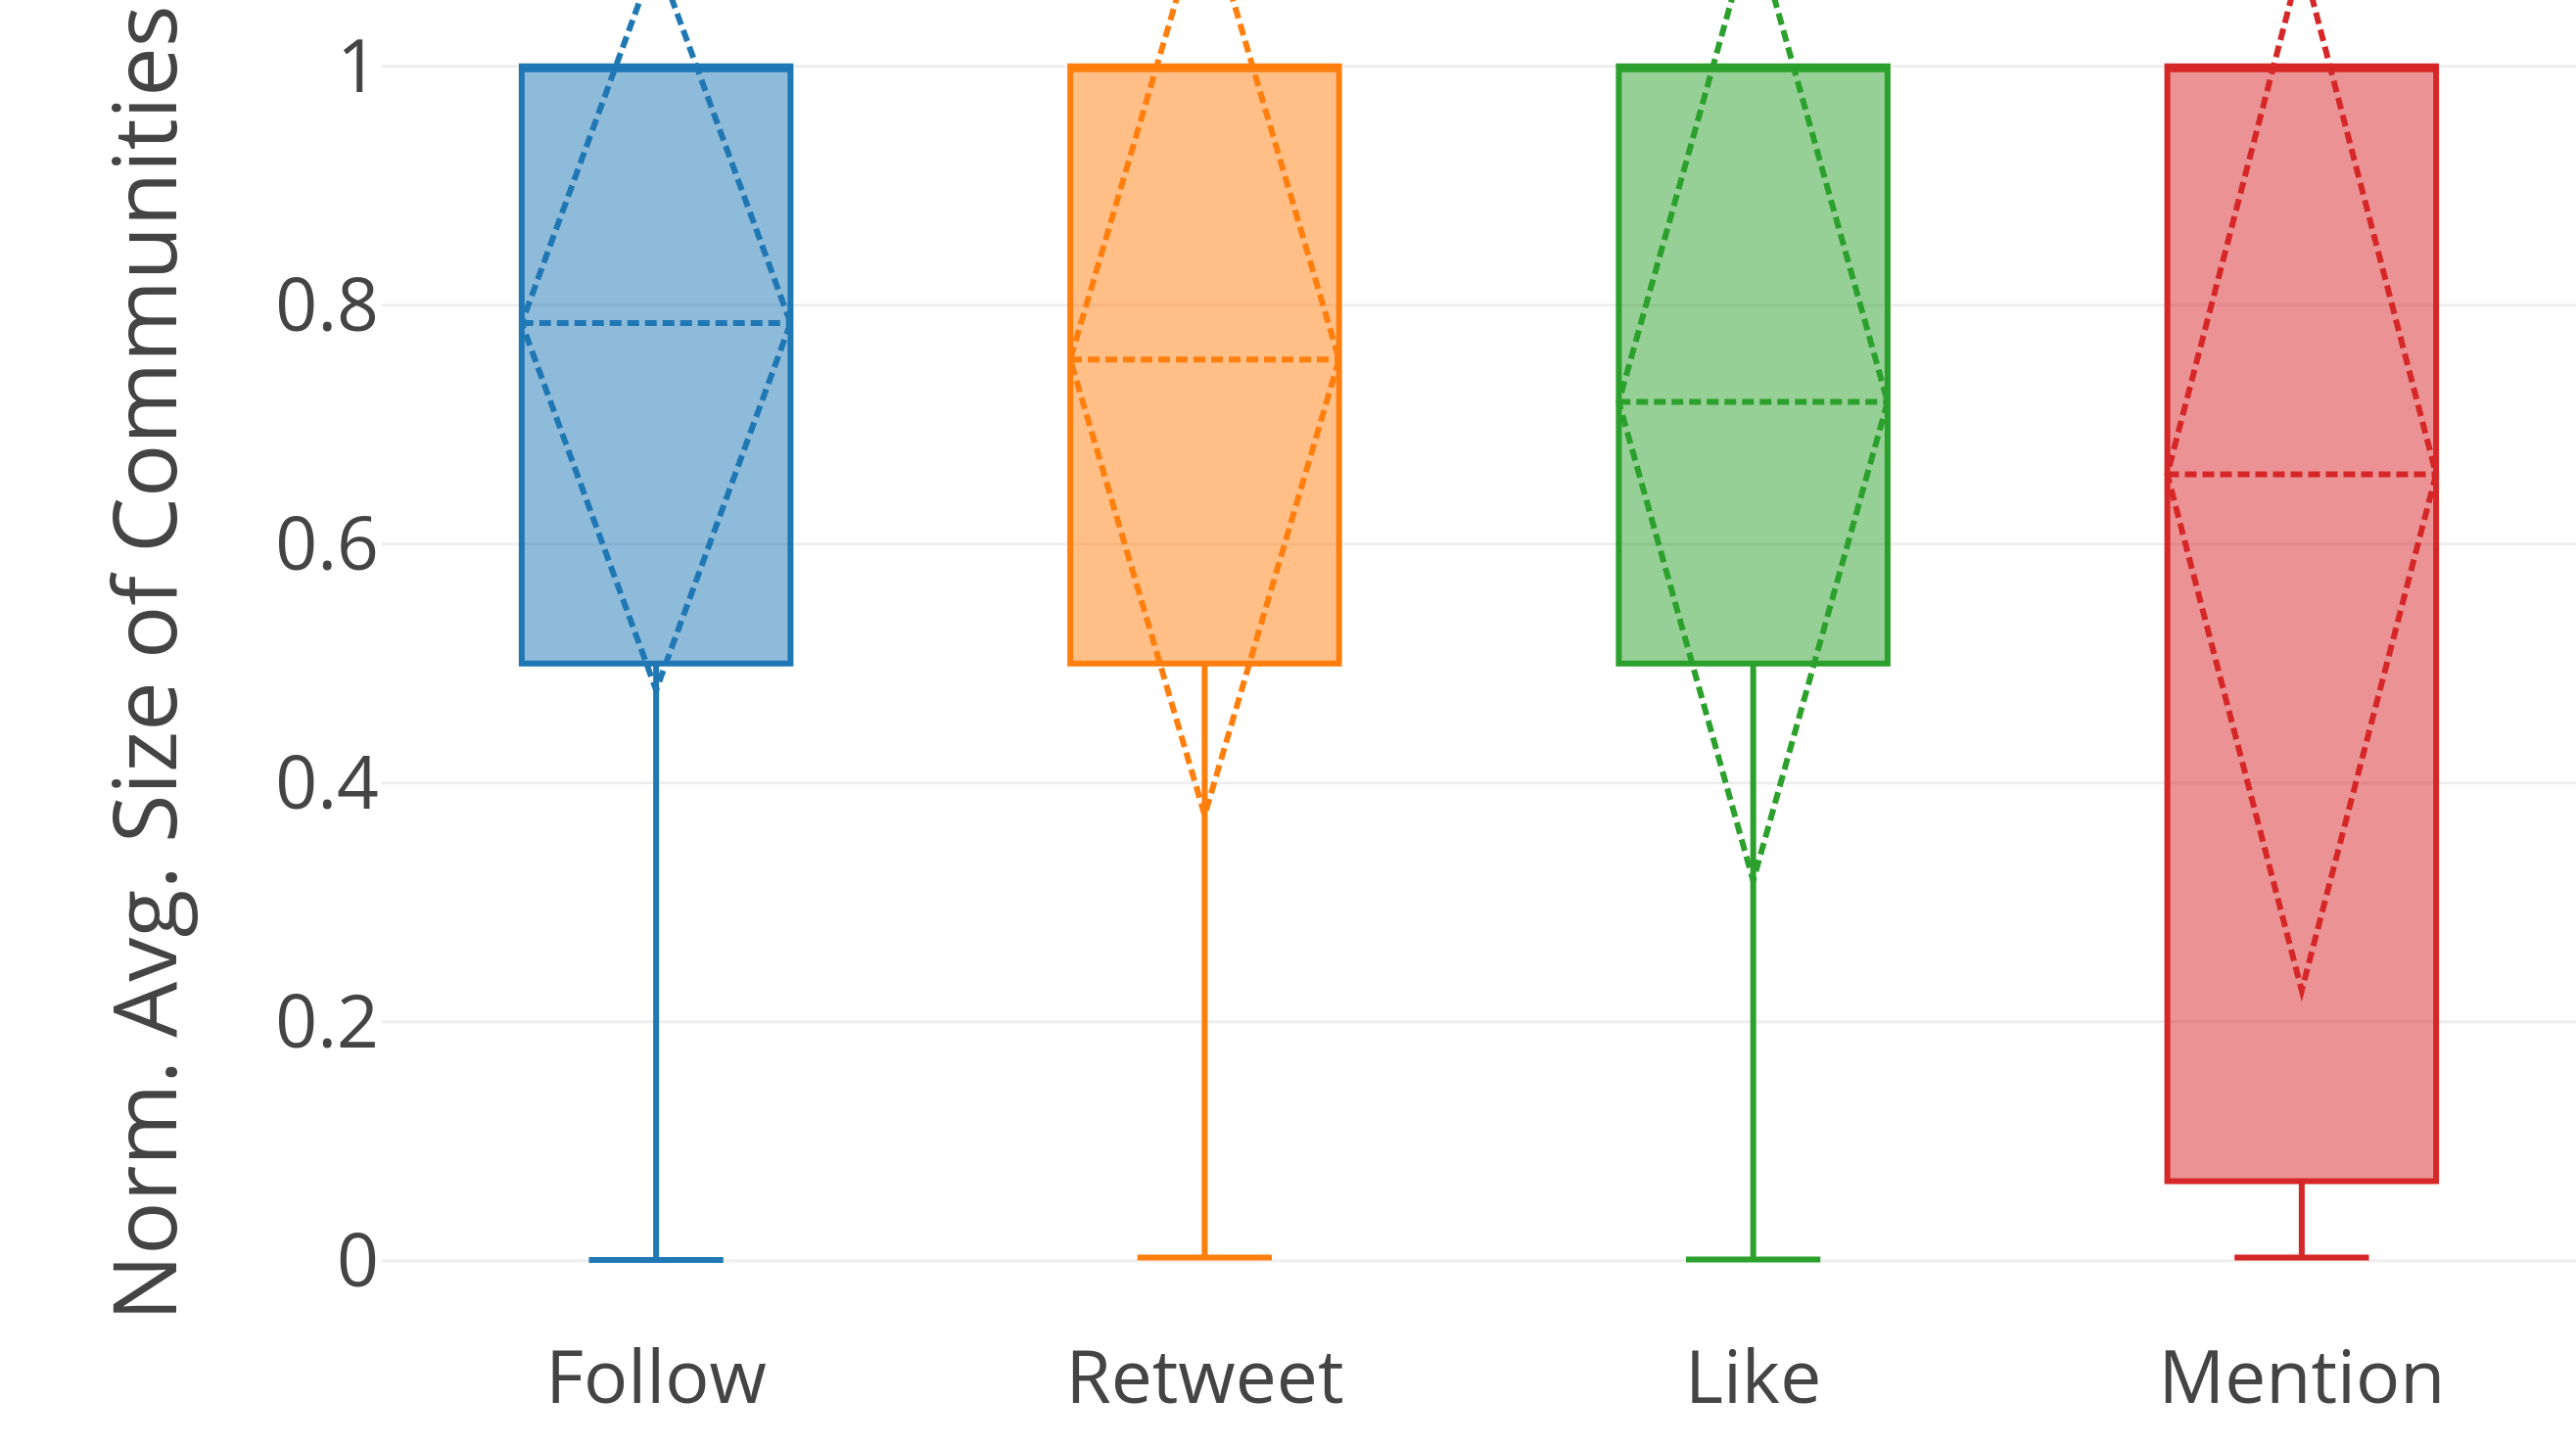
\includegraphics[width=0.47\textwidth]{fig/comm_stats/rak/comm_stats_norm_avg_comm_rak.png}
        \label{fig:comm_stats_avg_size_comm_rak}
    }
    \subfigure[INFOMAP]{
        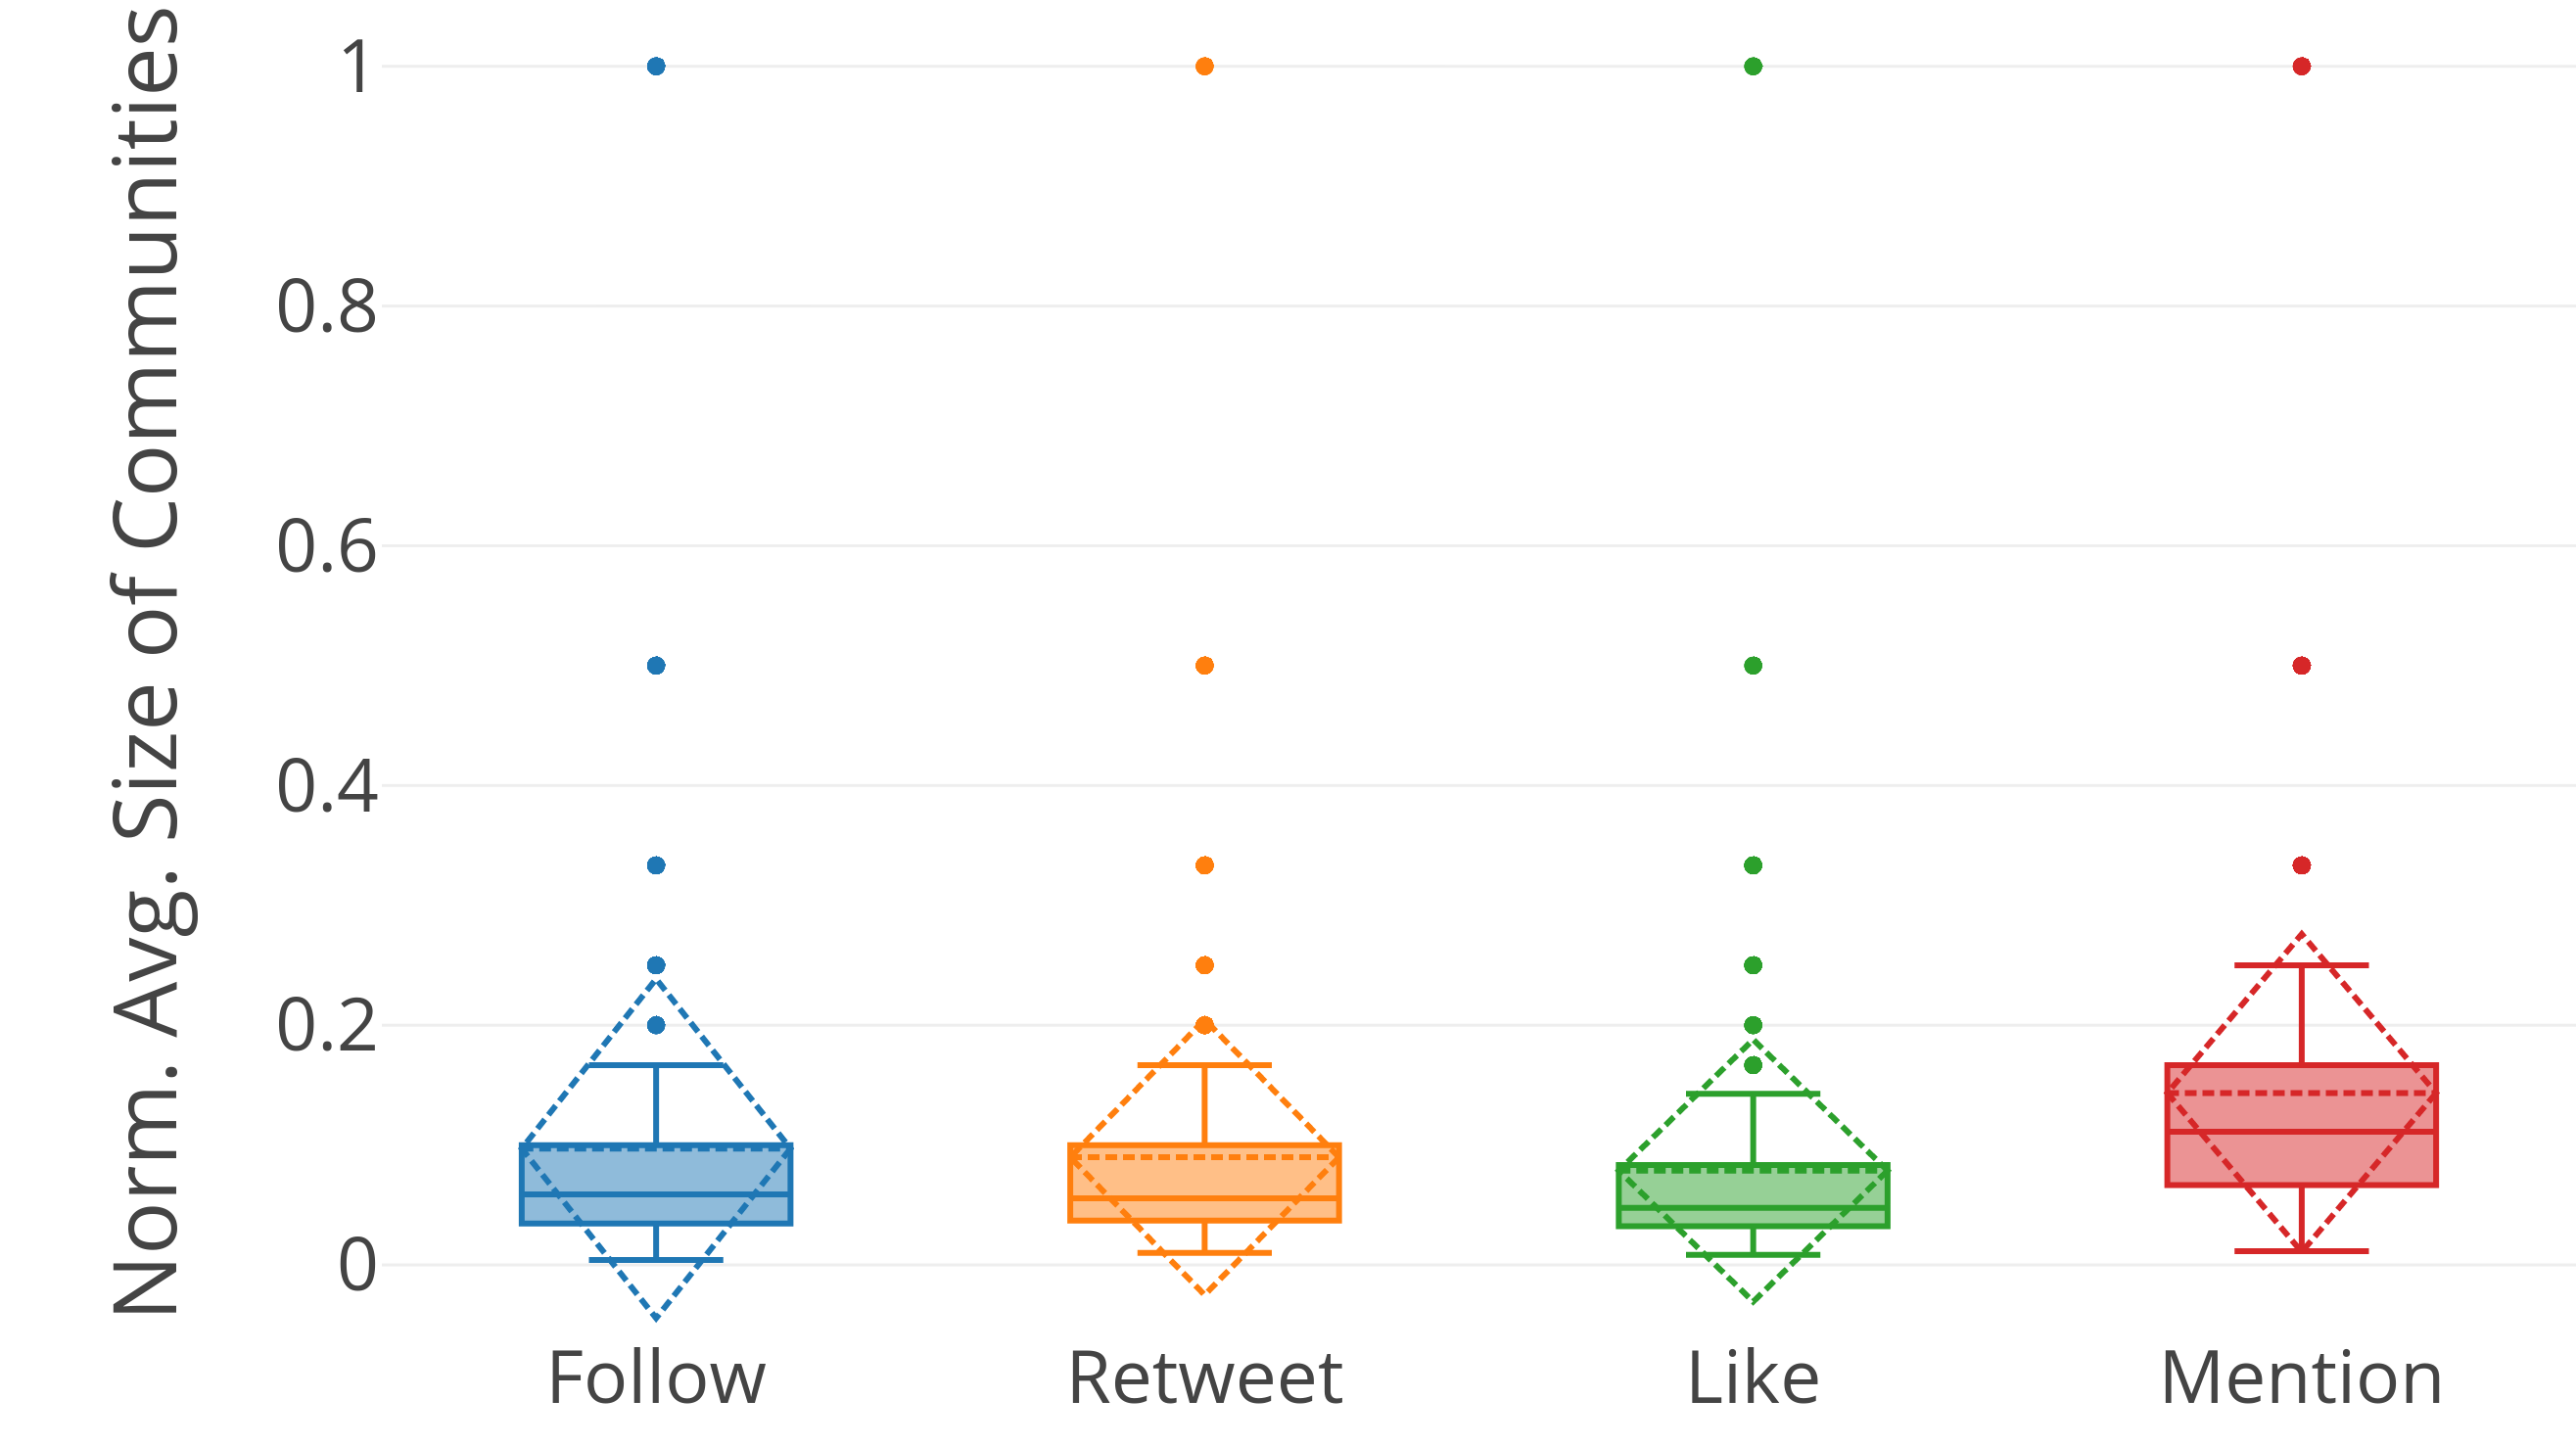
\includegraphics[width=0.47\textwidth]{fig/comm_stats/infomap/comm_stats_norm_avg_comm_infomap.png}
        \label{fig:comm_stats_avg_size_comm_infomap}
    } \\
    \subfigure[COPRA]{
        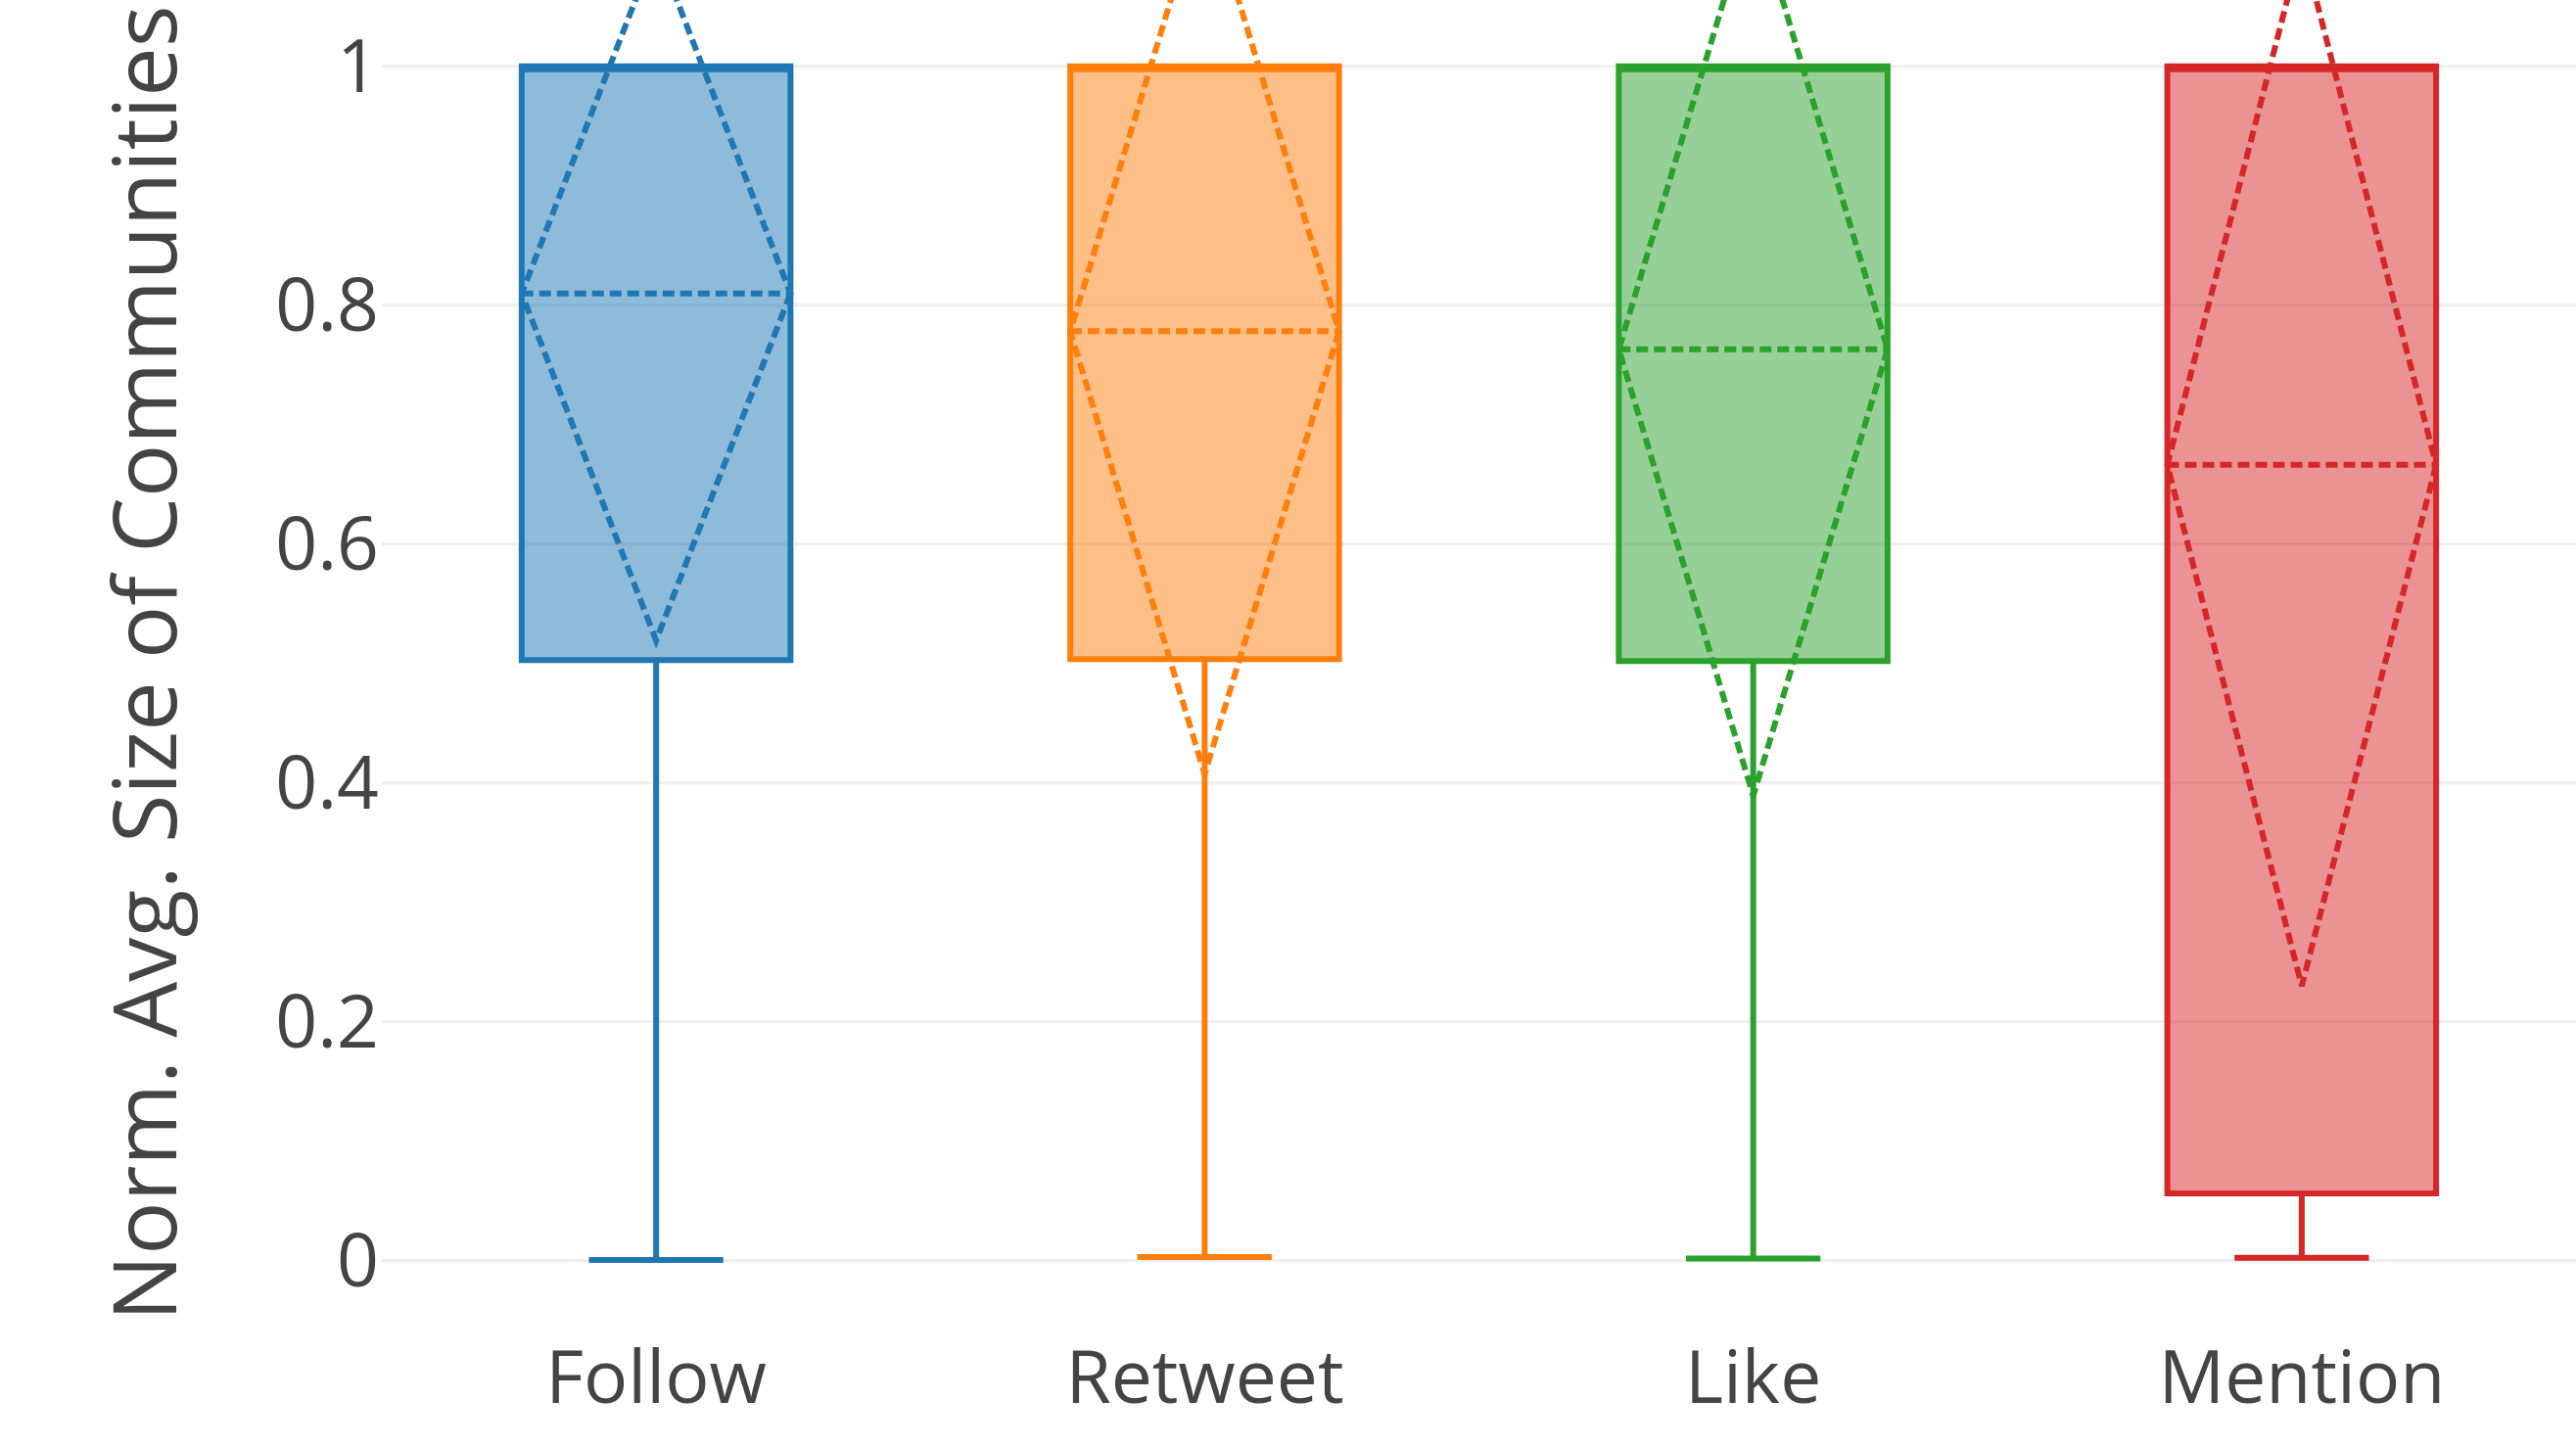
\includegraphics[width=0.47\textwidth]{fig/comm_stats/copra/comm_stats_norm_avg_comm_copra.png}
        \label{fig:comm_stats_avg_size_comm_copra}
    }
    \subfigure[OSLOM]{
        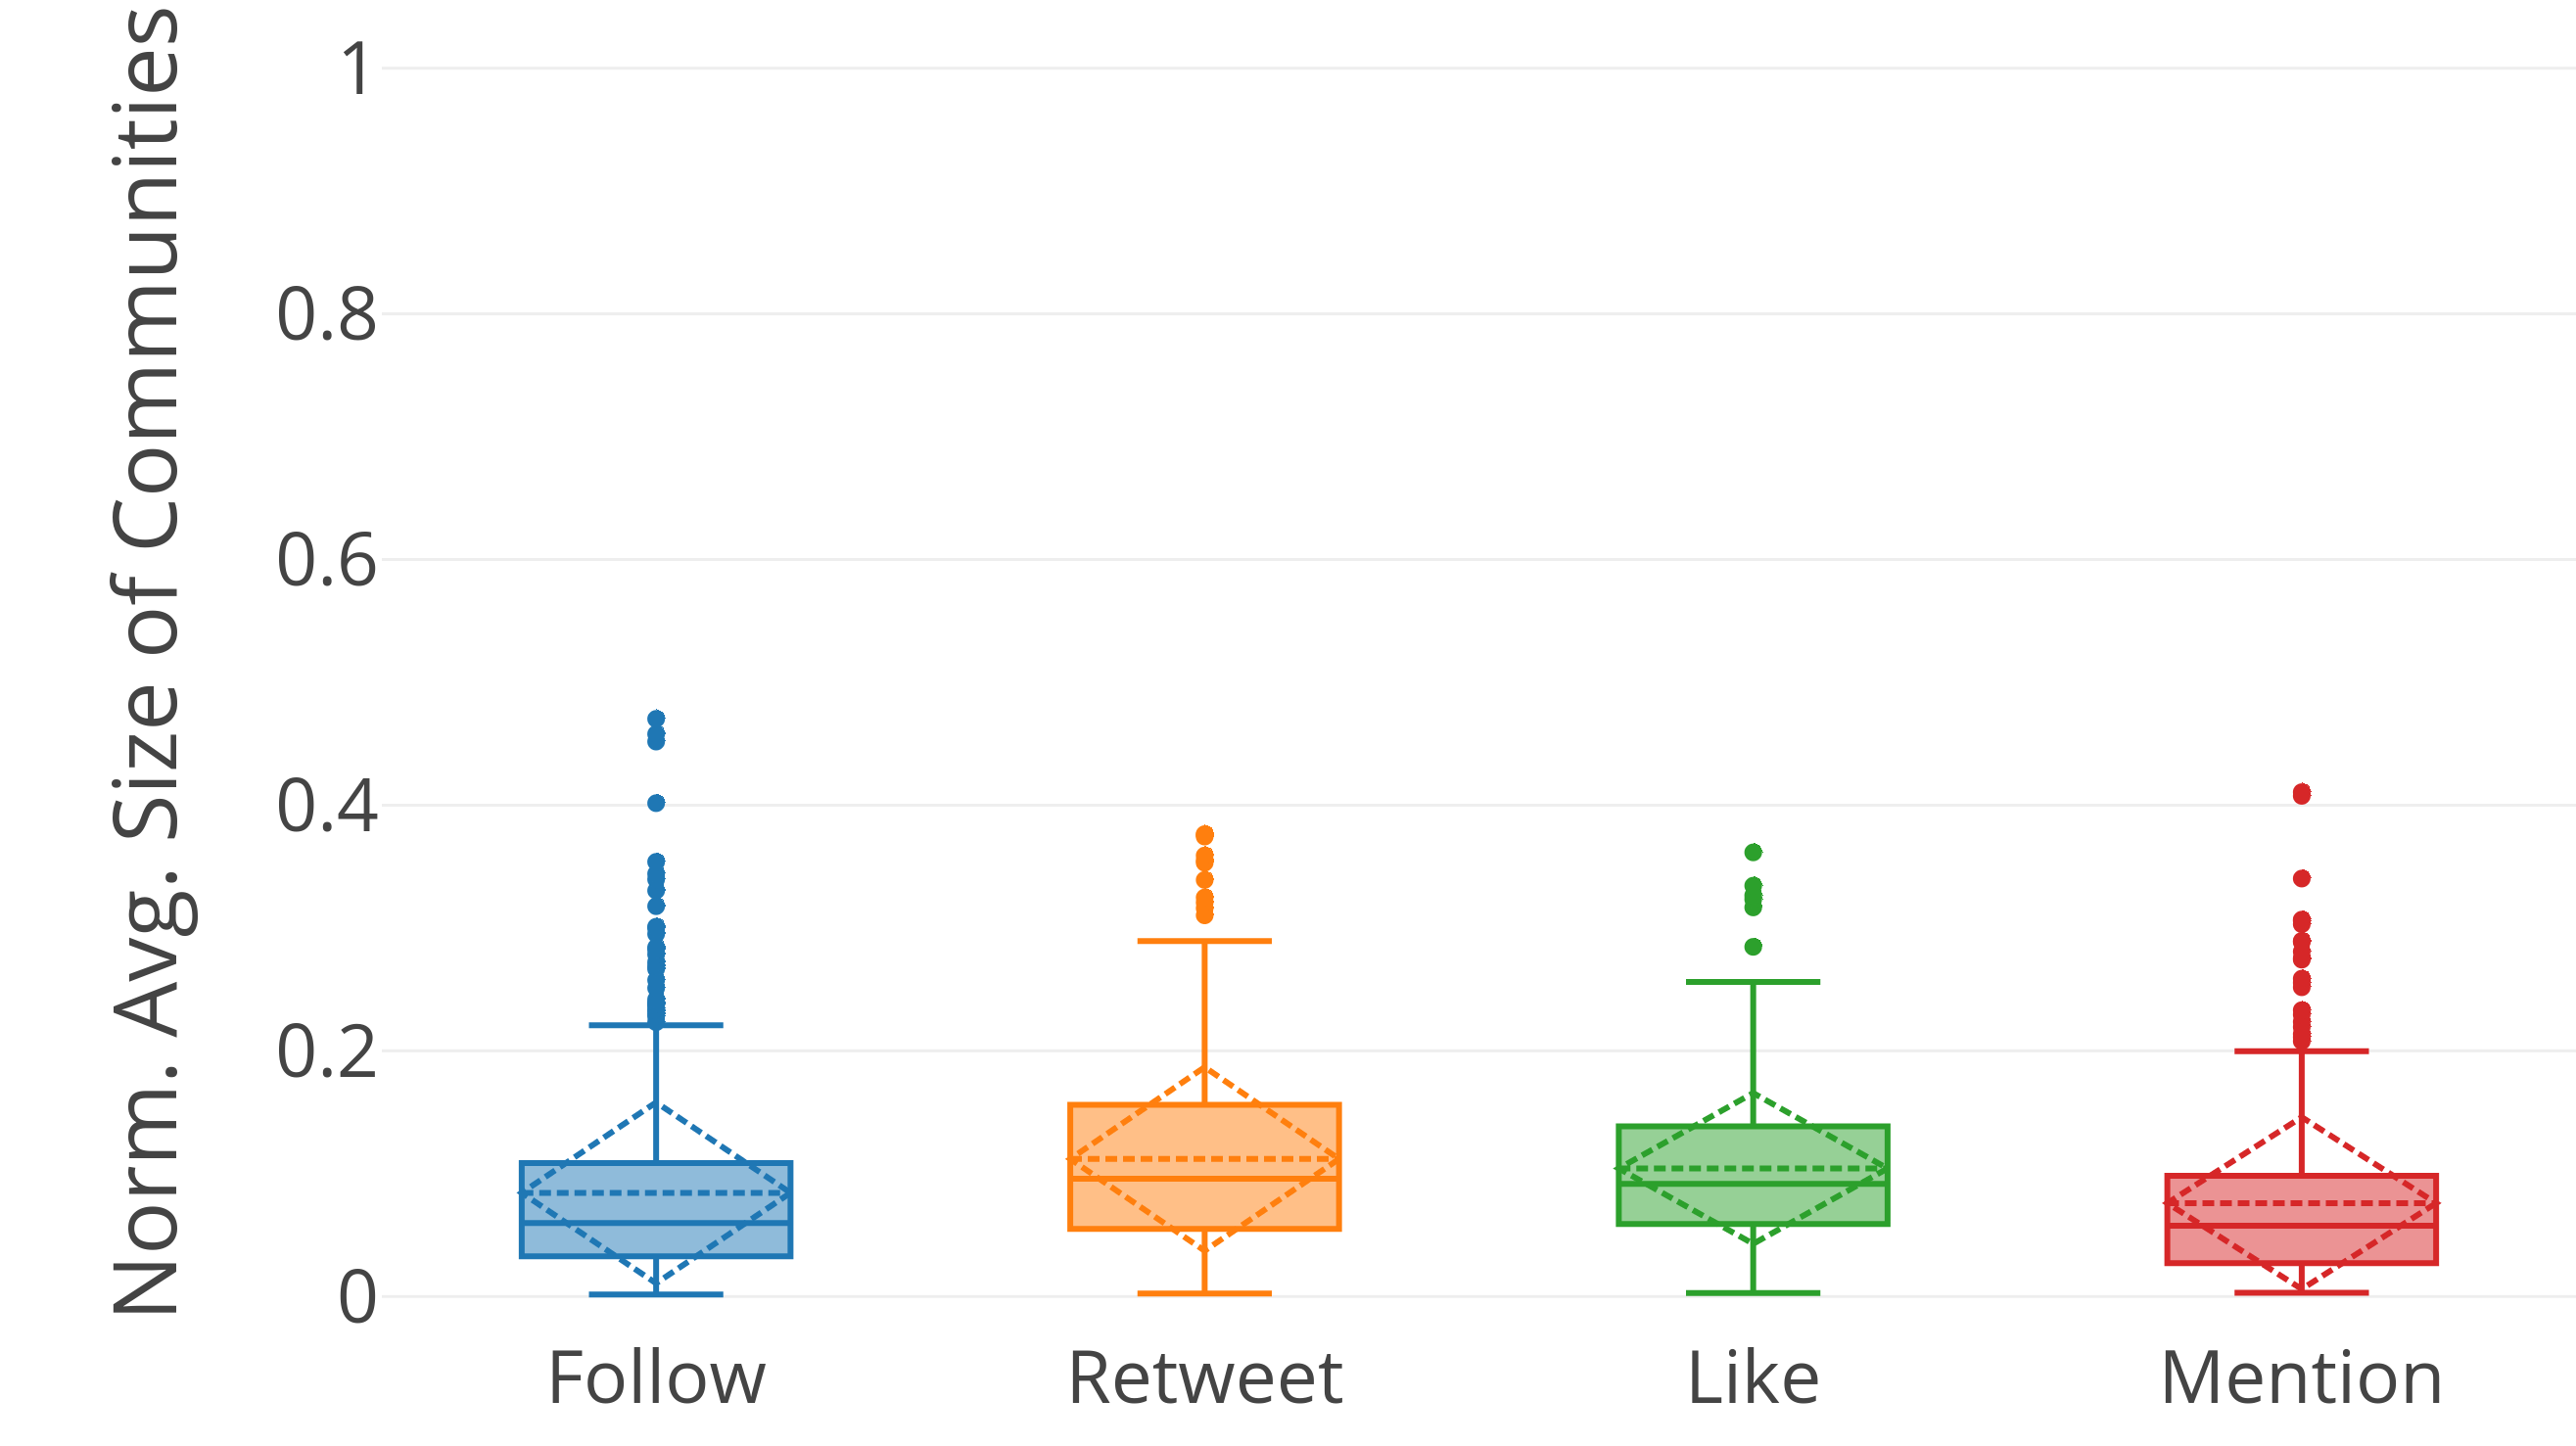
\includegraphics[width=0.47\textwidth]{fig/comm_stats/oslom/comm_stats_norm_avg_comm_oslom.png}
        \label{fig:comm_stats_avg_size_comm_oslom}
    }
    \caption{Average size of communities detected in each layer normalized by the order of the ego networks.}
    \label{fig:comm_stats_avg_size_comm}
\end{figure}



\begin{figure}[h!tb]
    \centering
    \subfigure[RAK]{
        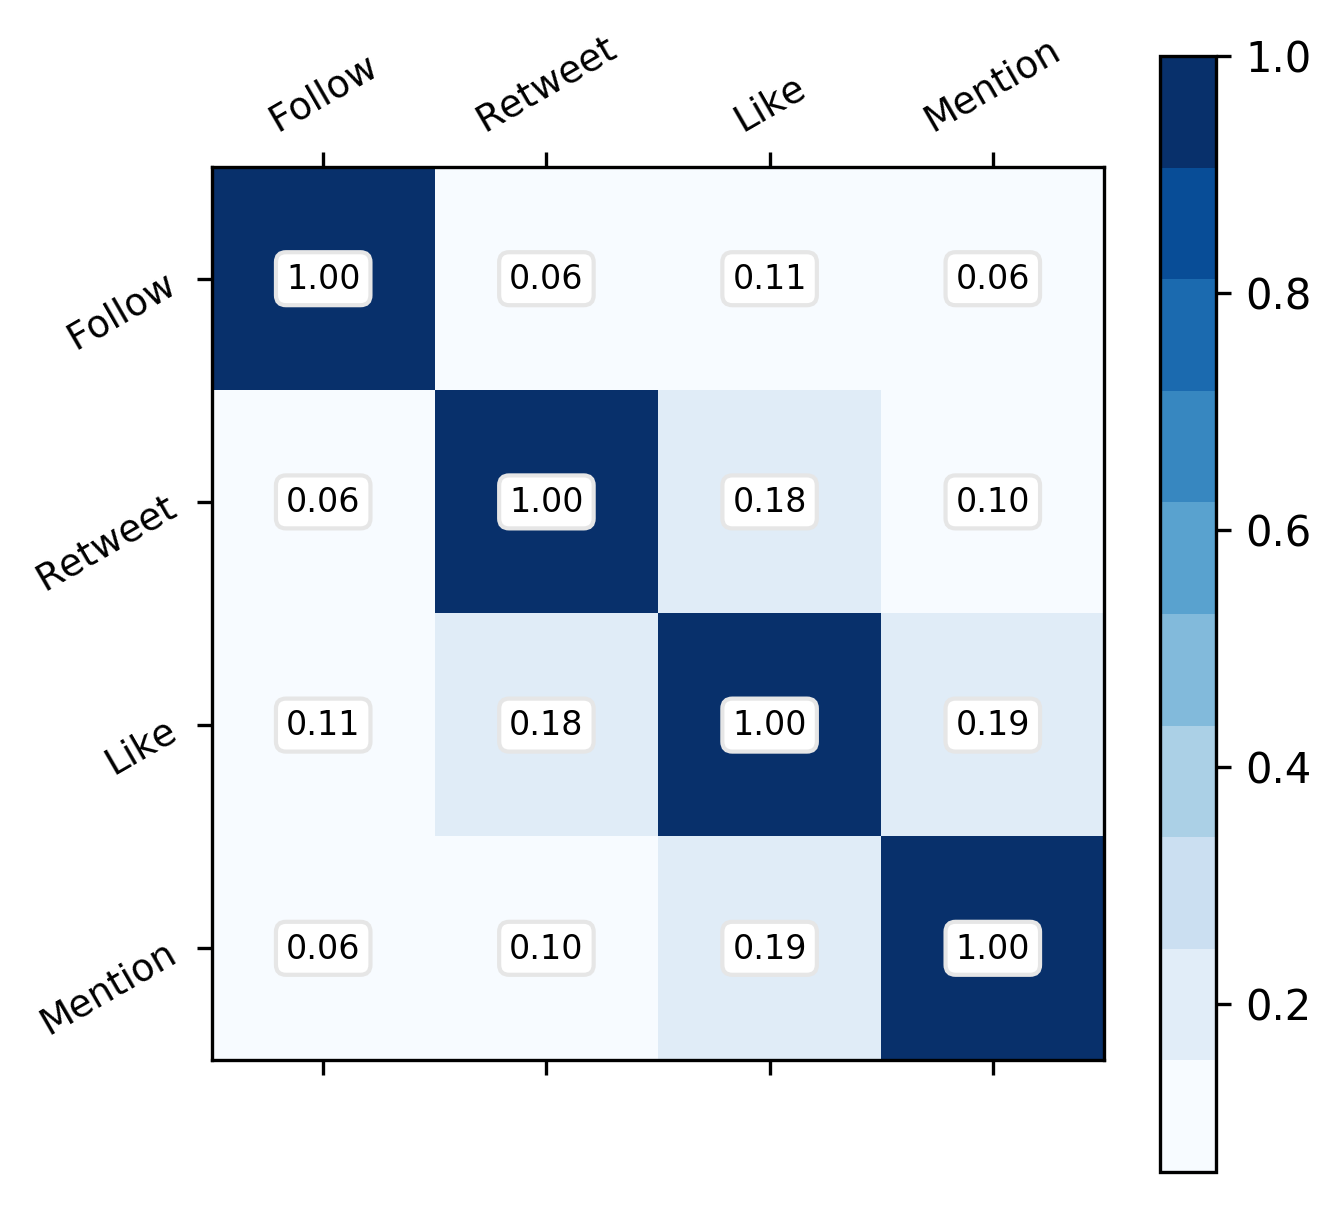
\includegraphics[width=0.47\textwidth]{fig/comm_stats/rak/n_comm_correlation_spearman.png}
        \label{fig:comm_stats_n_comm_correlation_rak}
    }
    \subfigure[INFOMAP]{
        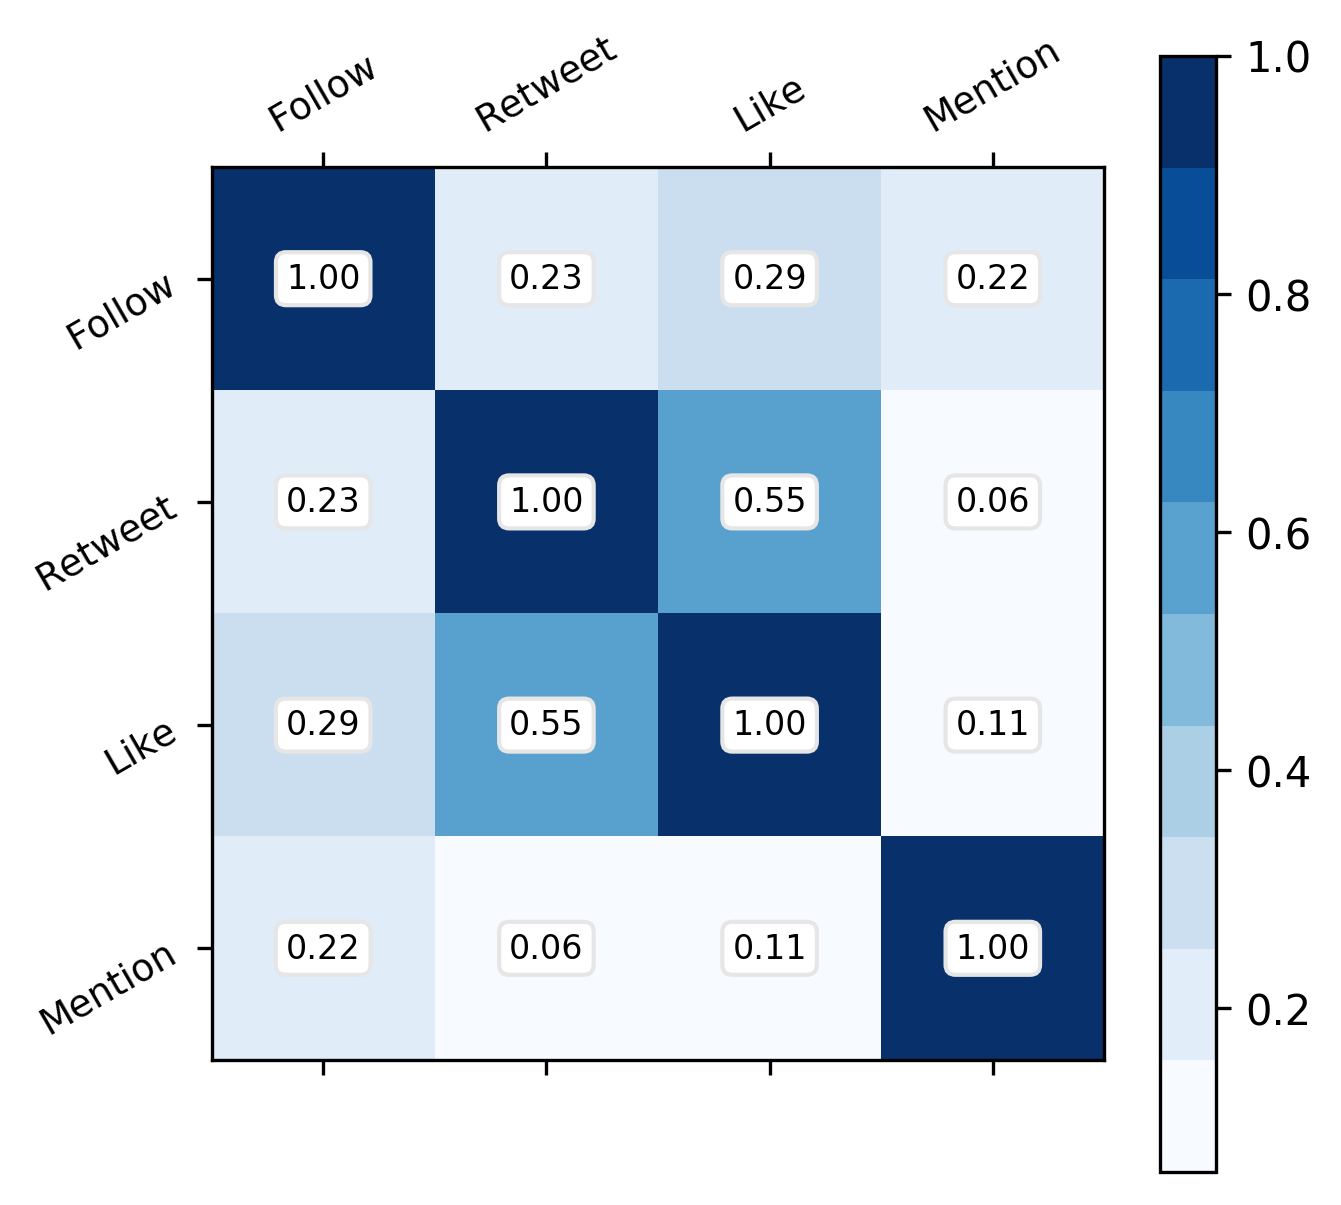
\includegraphics[width=0.47\textwidth]{fig/comm_stats/infomap/n_comm_correlation_spearman.png}
        \label{fig:comm_stats_n_comm_correlation_infomap}
    } \\
    \subfigure[COPRA]{
        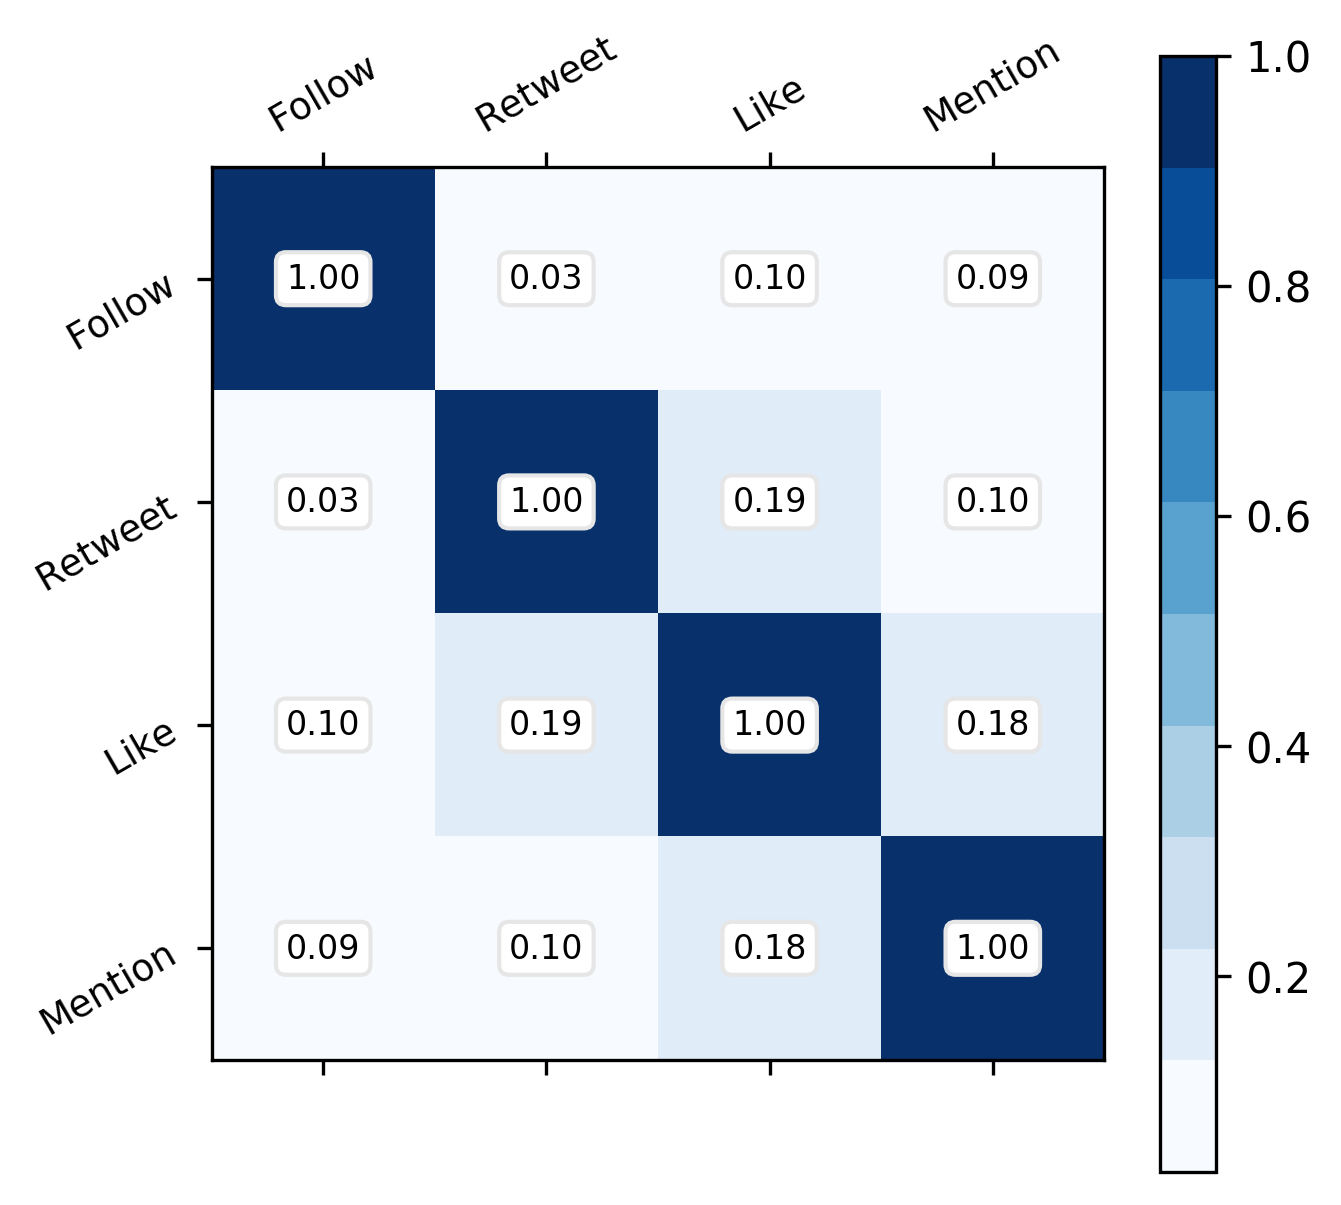
\includegraphics[width=0.47\textwidth]{fig/comm_stats/copra/n_comm_correlation_spearman.png}
        \label{fig:comm_stats_n_comm_correlation_copra}
    }
    \subfigure[OSLOM]{
        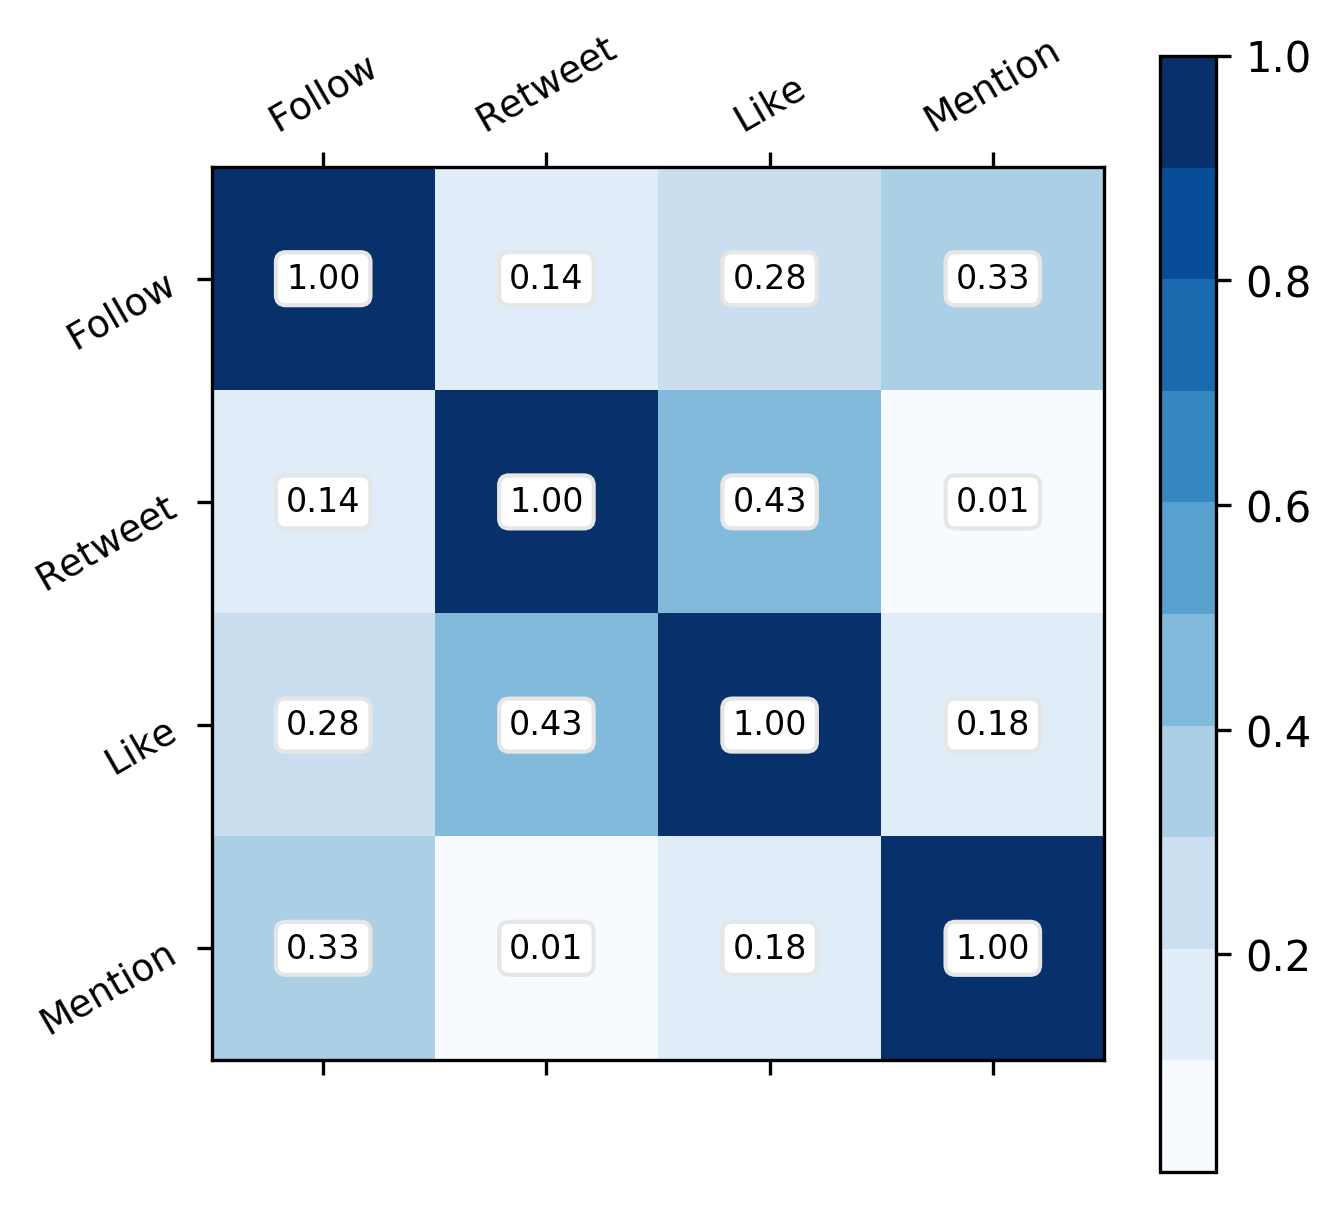
\includegraphics[width=0.47\textwidth]{fig/comm_stats/oslom/n_comm_correlation_spearman.png}
        \label{fig:comm_stats_n_comm_correlation_oslom}
    }
    \caption{Spearman's correlation between the layers for the number of communities detected in each layer.}
    \label{fig:comm_stats_n_comm_correlation}
\end{figure}

Figure \ref{fig:comm_stats_avg_size_comm} displays a boxplot with mean values for the size of the communities found in each ego network. This value is normalized by the size of the ego networks. It is noted that the RAK \ref{fig:comm_stats_avg_size_comm_rak} and COPRA \ref{fig:comm_stats_avg_size_comm_copra} algorithms present the highest values, indicating that, according to these algorithms, for most ego networks there is a very large single community formed by almost all or all of the vertices of the graph, although the mention layer greater variation. As for the algorithms INFOMAP \ref{fig:comm_stats_avg_size_comm_infomap} and OSLOM \ref{fig:comm_stats_avg_size_comm_oslom}, the average community sizes are low, which indicates a larger number of communities detected by these algorithms and, in the case of OSLOM, which detects vertex overlap, communities are also small in relation to the network ego. The interesting thing is that for all the algorithms the results between the layers present little variation.



Figure \ref{fig:comm_stats_n_comm_correlation} shows the Spearman{'}s Correlation between pairs of layers regarding the number of communities detected. We found weak or moderate correlations between most pairs of layers, except for the pair (retweet, like). As happens in many of the previous analysis, this pair also has affinity in relation to the number of communities. However, despite this affinity, as we reported in Section \ref{sec:net_structure}, for many egos these two pair of layers have different set of vertices and different of edges which makes their communities to be also distinct from each other.  

\begin{figure}[h!tb]
    \centering
    \subfigure[RAK]{
        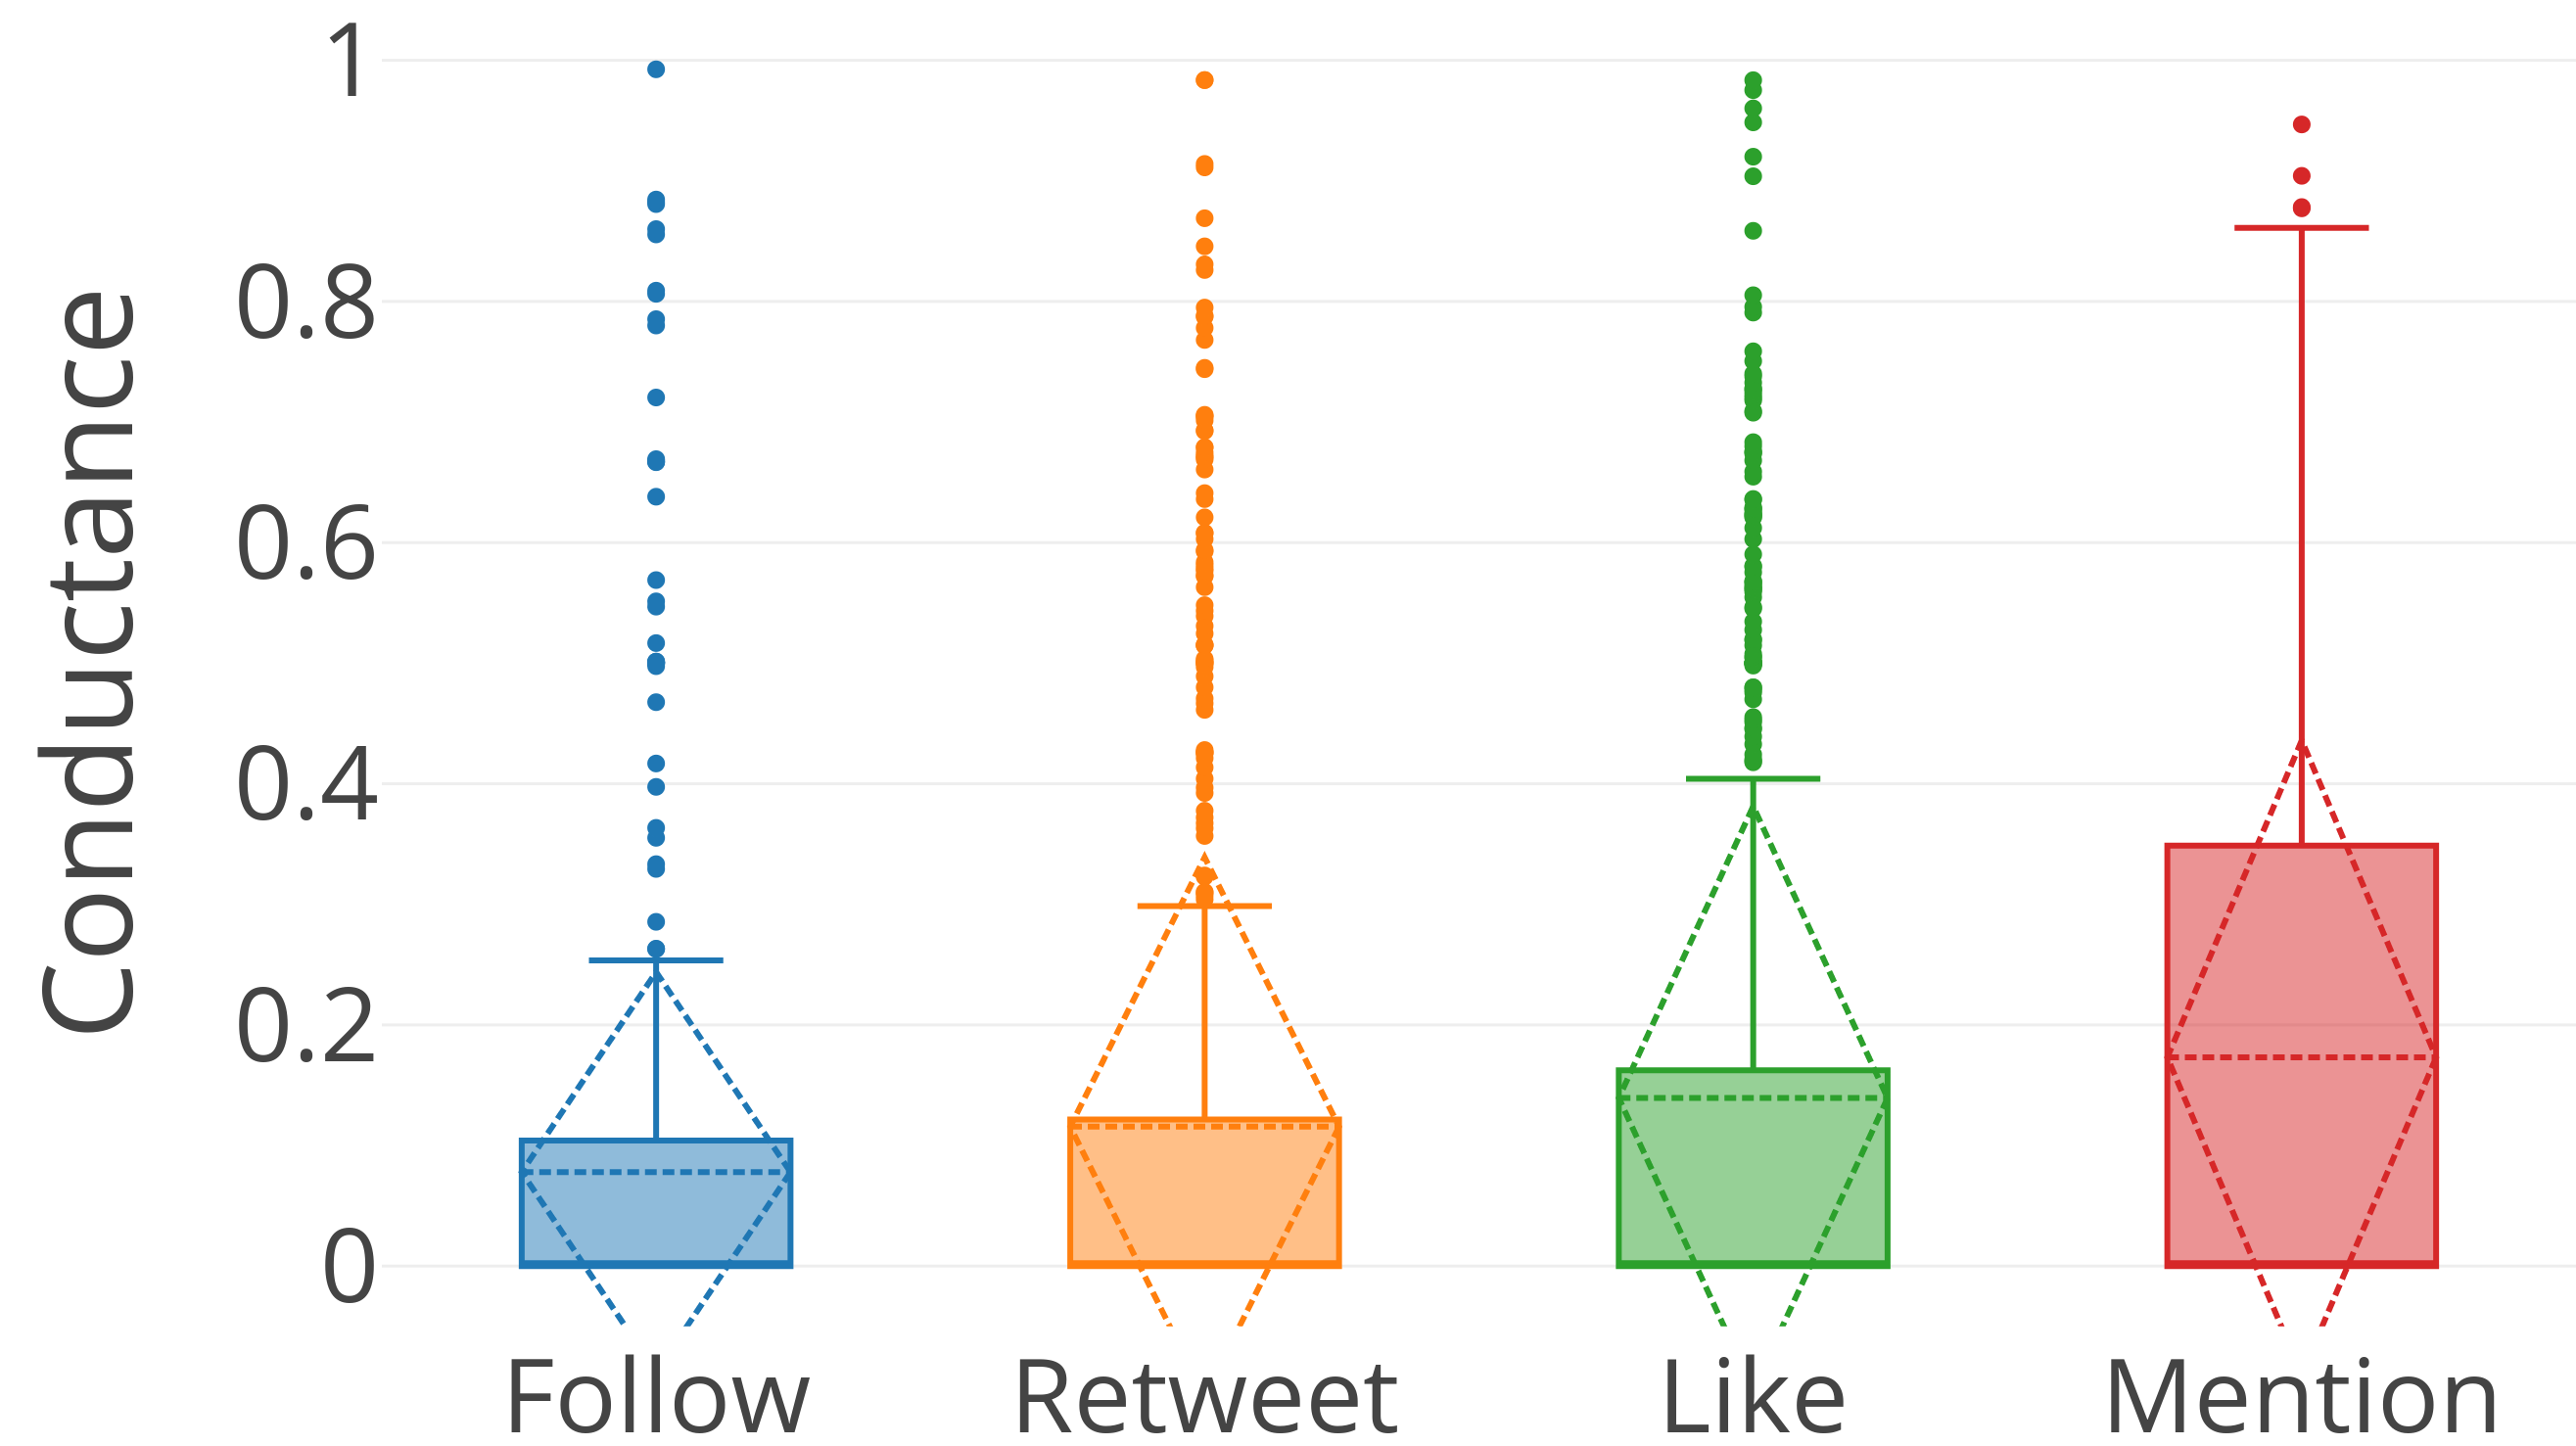
\includegraphics[width=0.47\textwidth]{fig/comm_metrics/rak/rak_conductance.png}
        \label{fig:comm_metrics_conductance_rak}
    }
    \subfigure[INFOMAP]{
        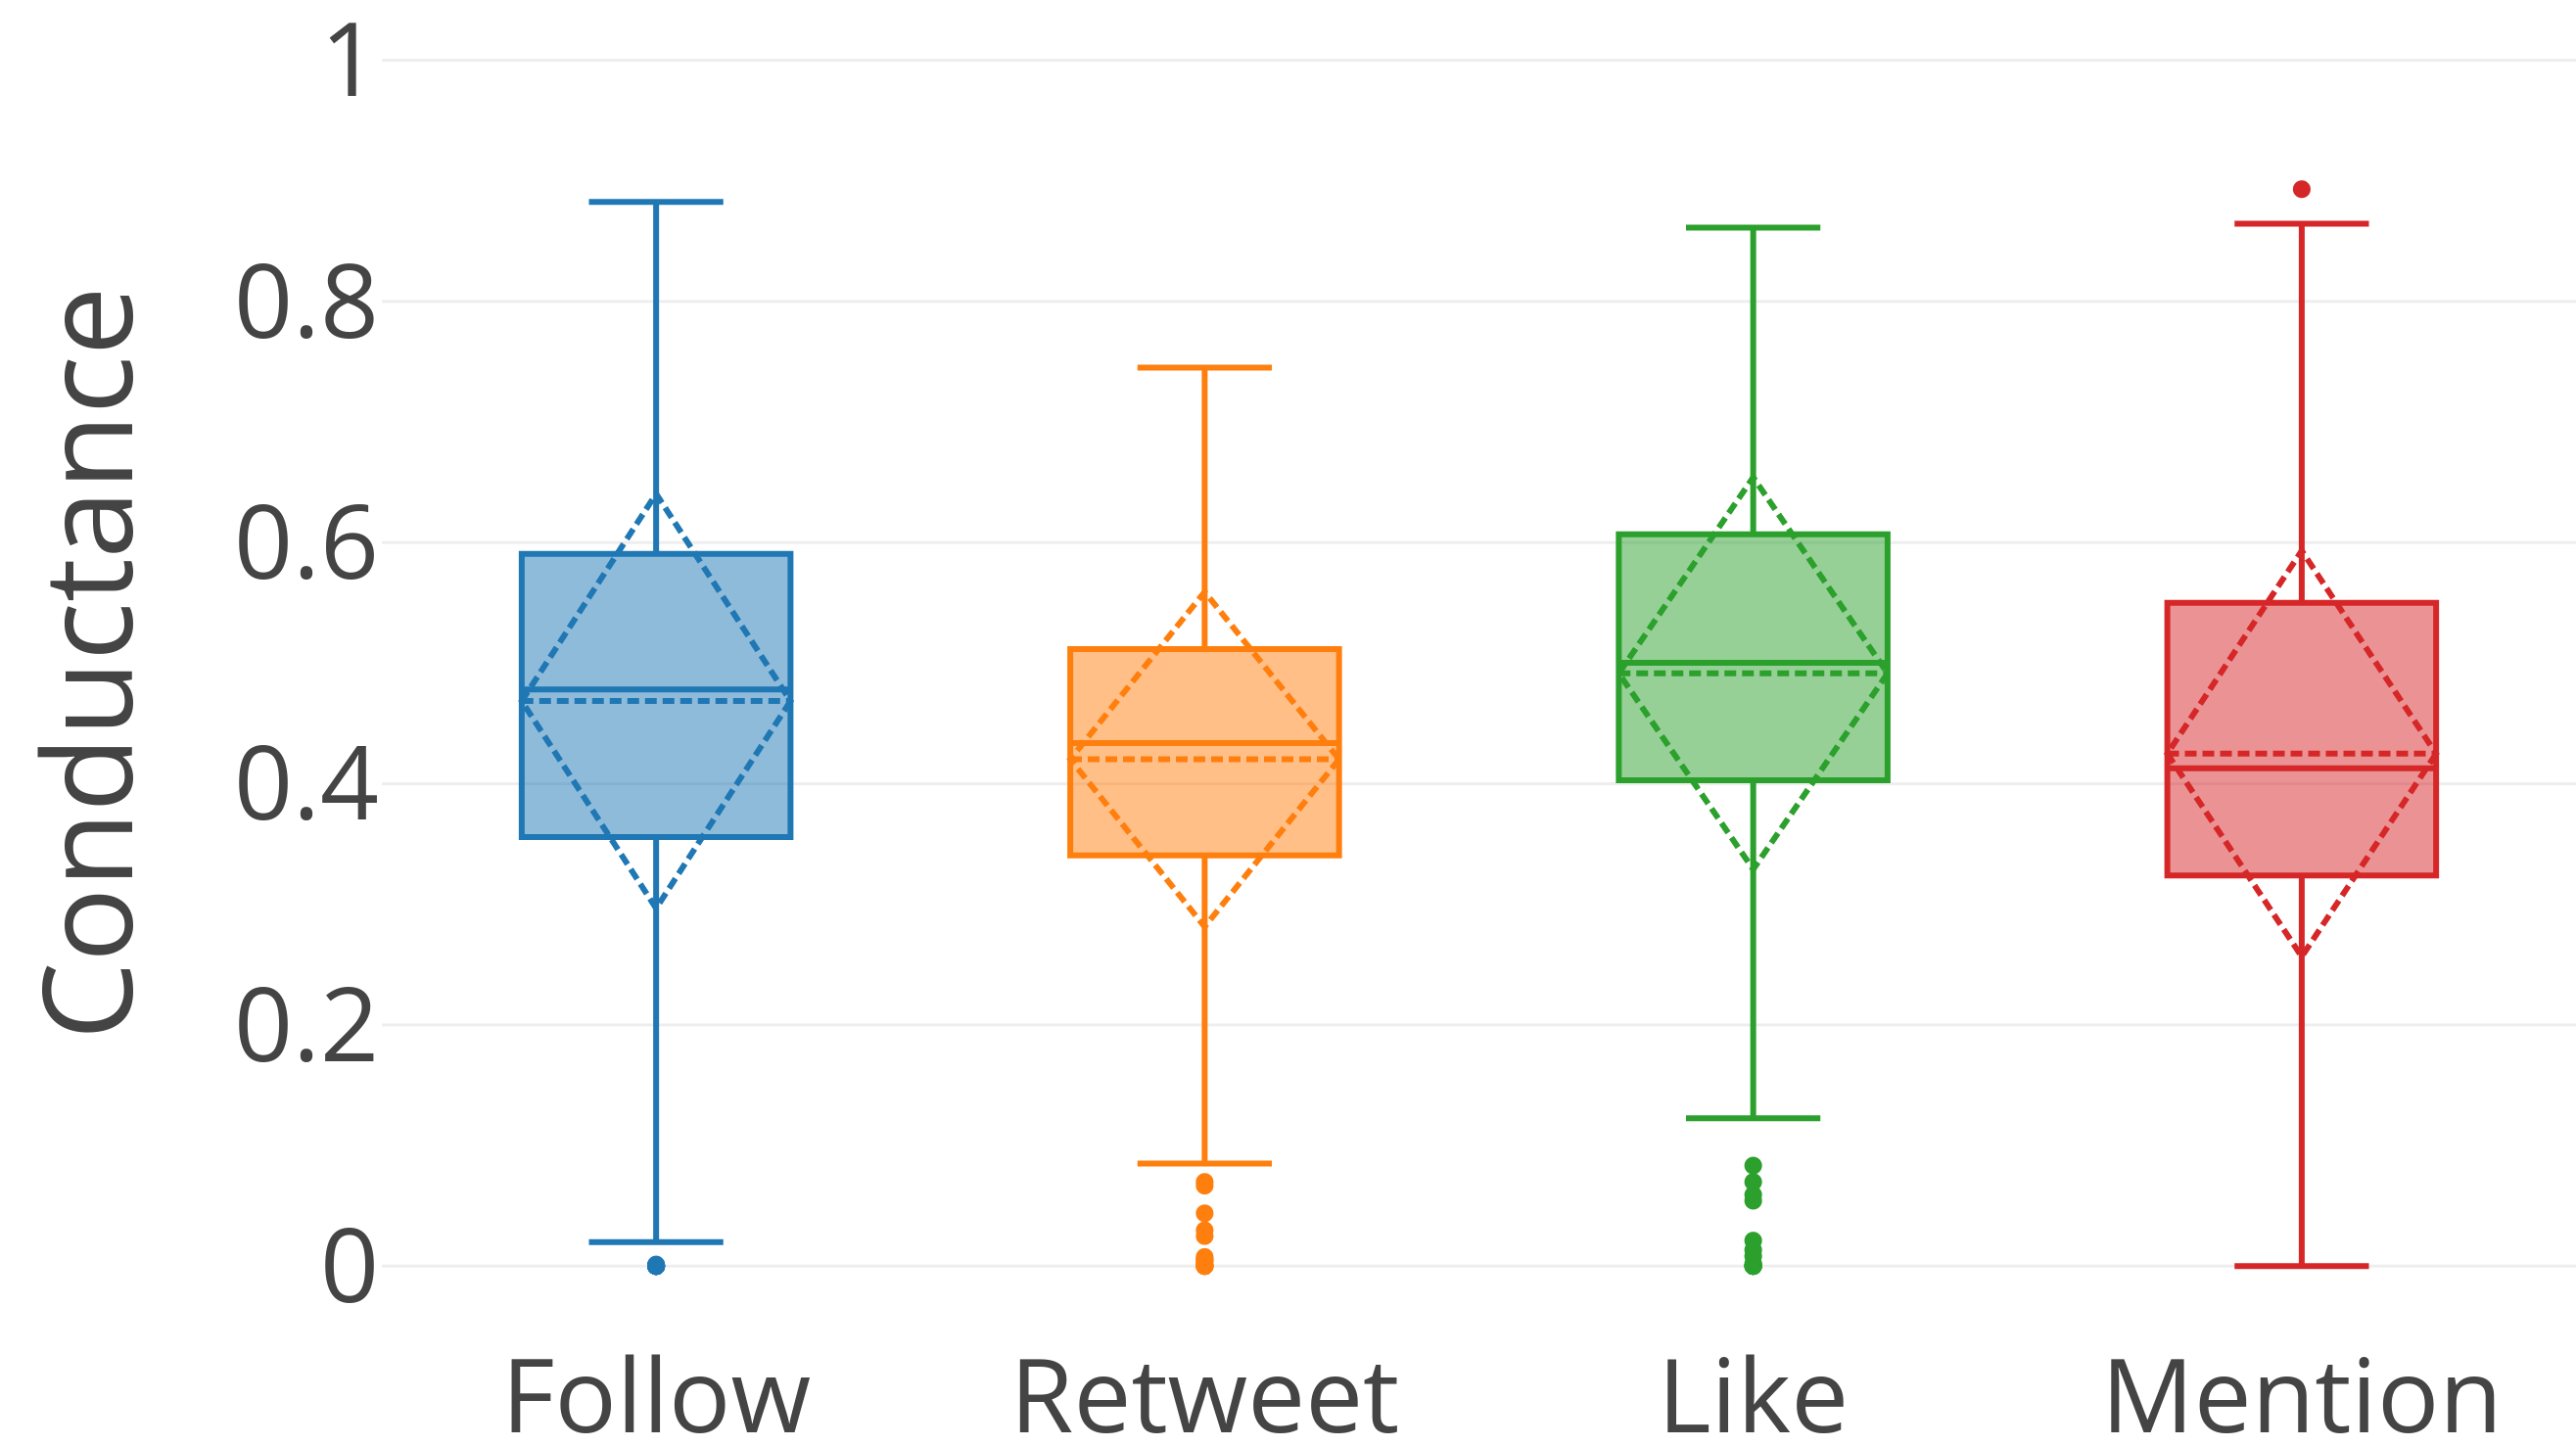
\includegraphics[width=0.47\textwidth]{fig/comm_metrics/infomap/infomap_conductance.png}
        \label{fig:comm_metrics_conductance_infomap}
    } \\
    \subfigure[COPRA]{
        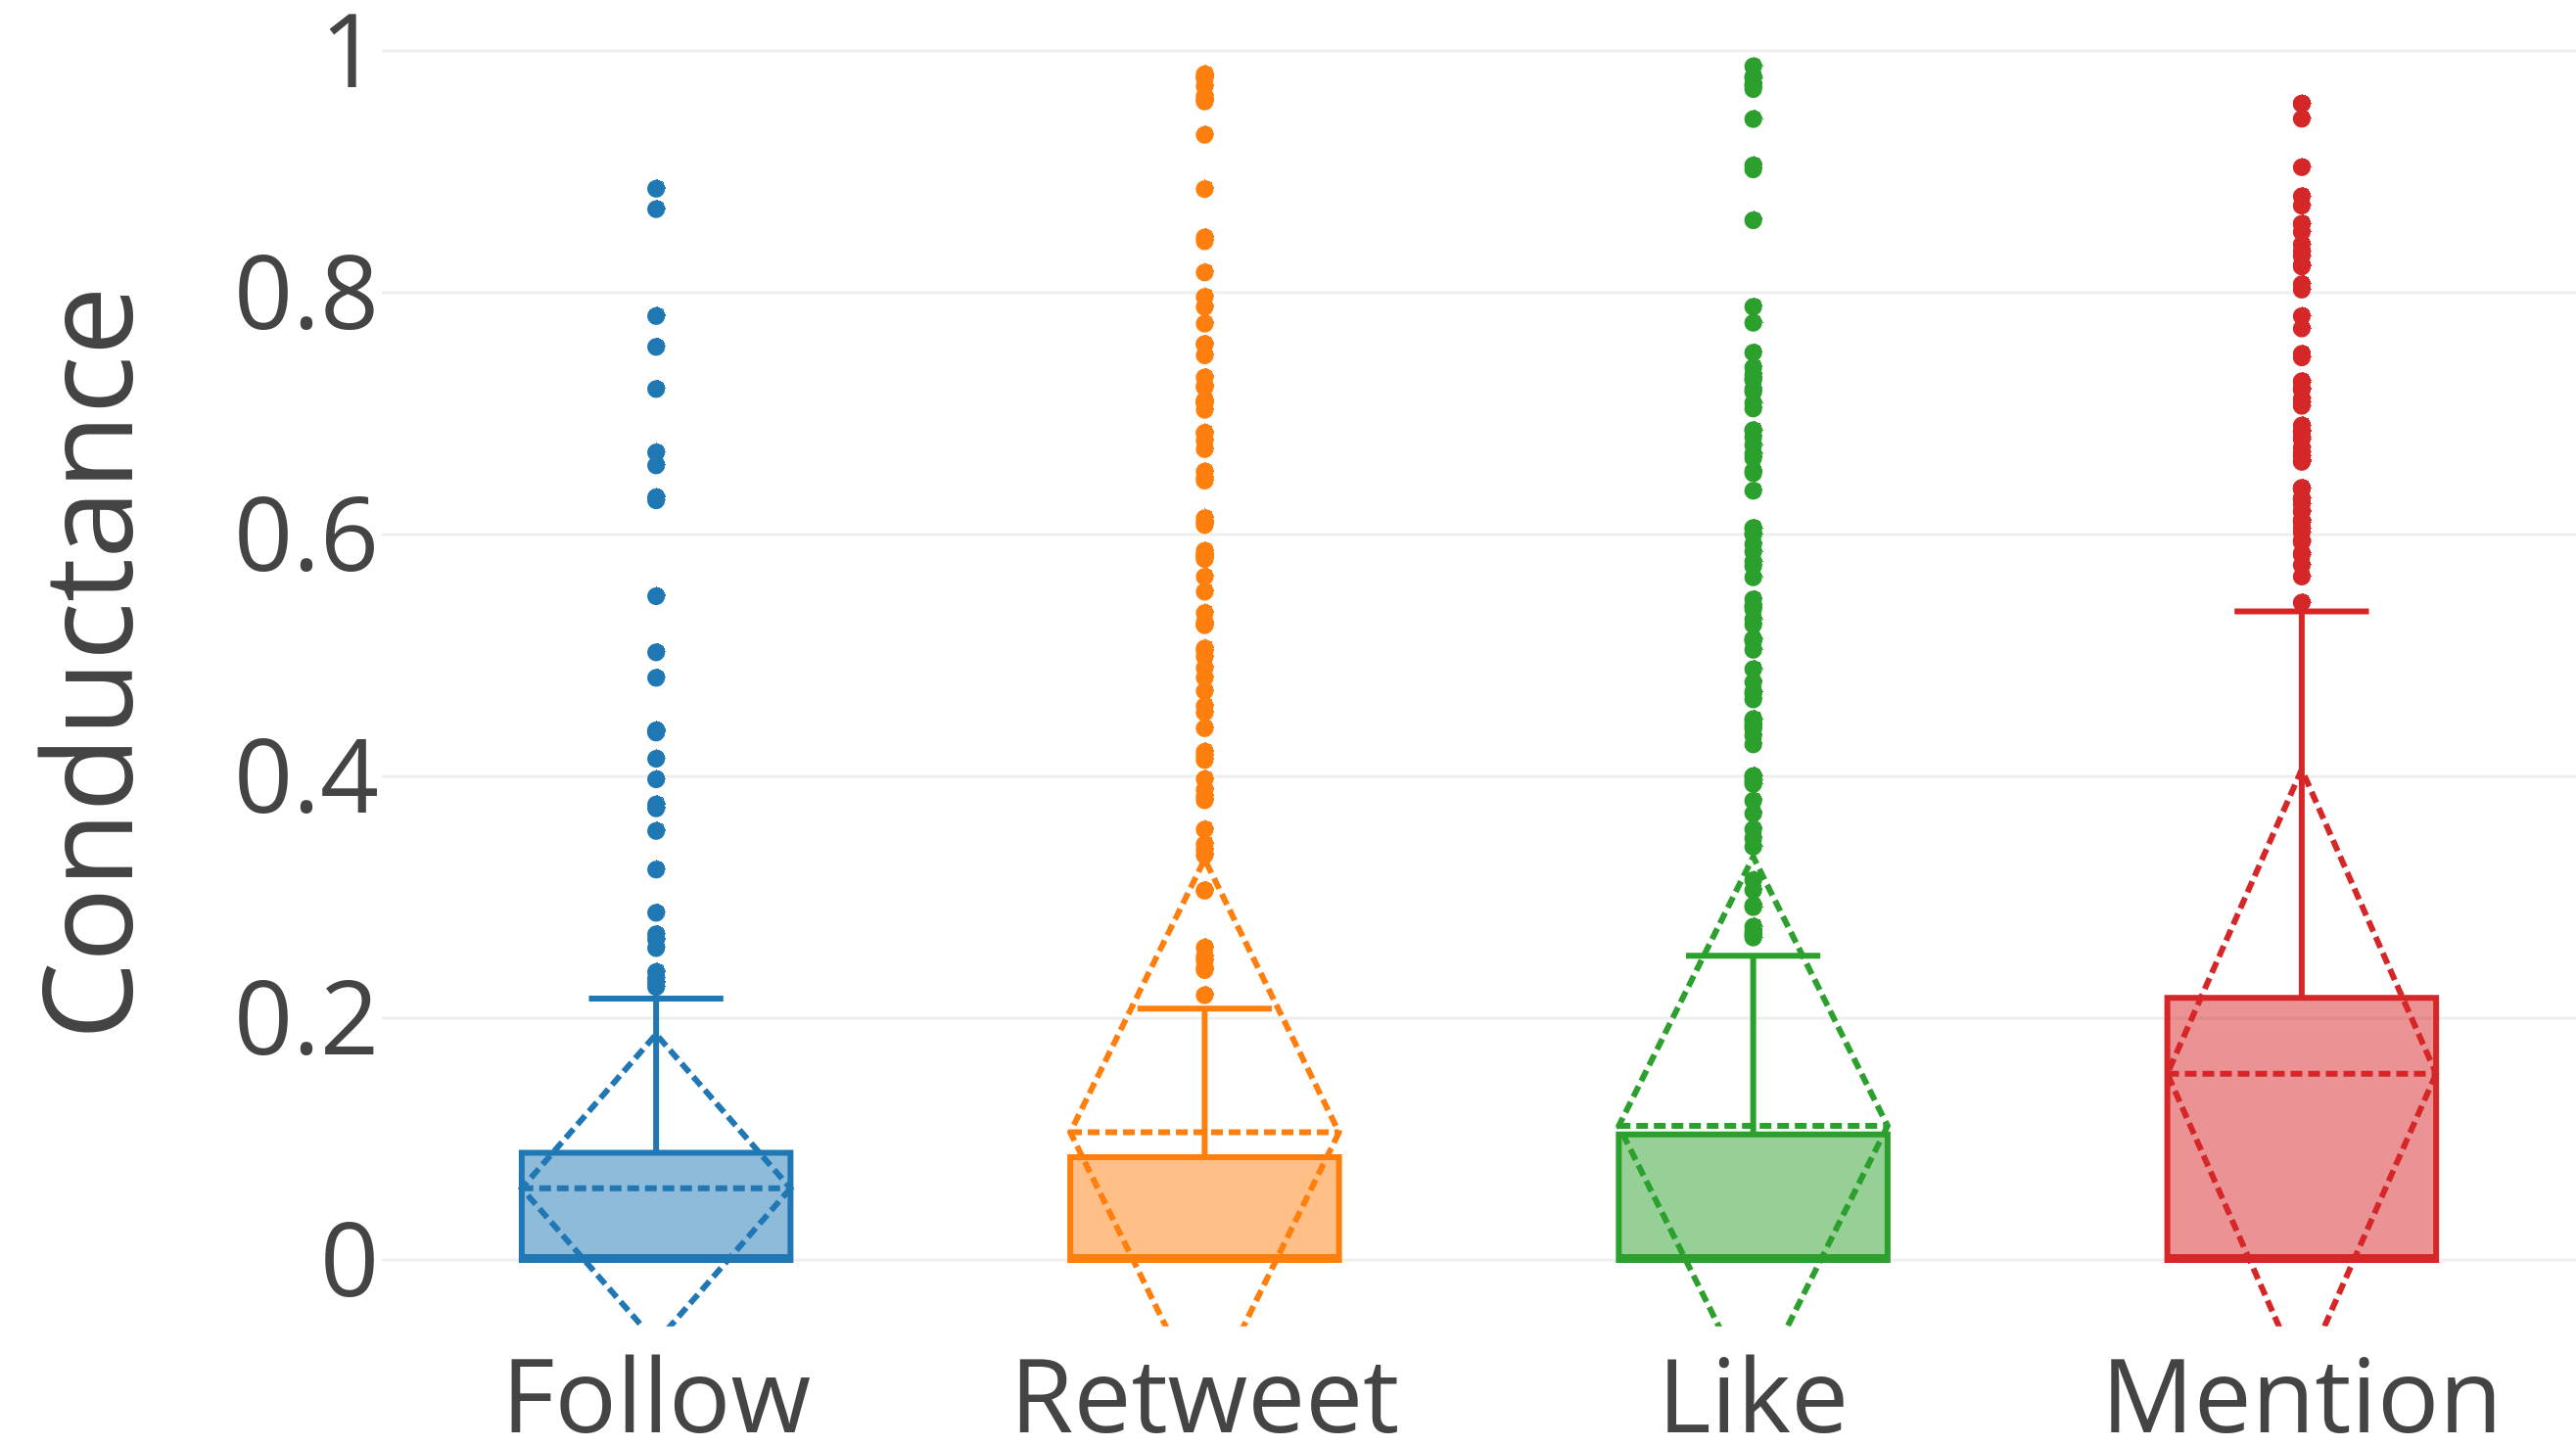
\includegraphics[width=0.47\textwidth]{fig/comm_metrics/copra/copra_conductance.png}
        \label{fig:comm_metrics_conductance_copra}
    }
    \subfigure[OSLOM]{
        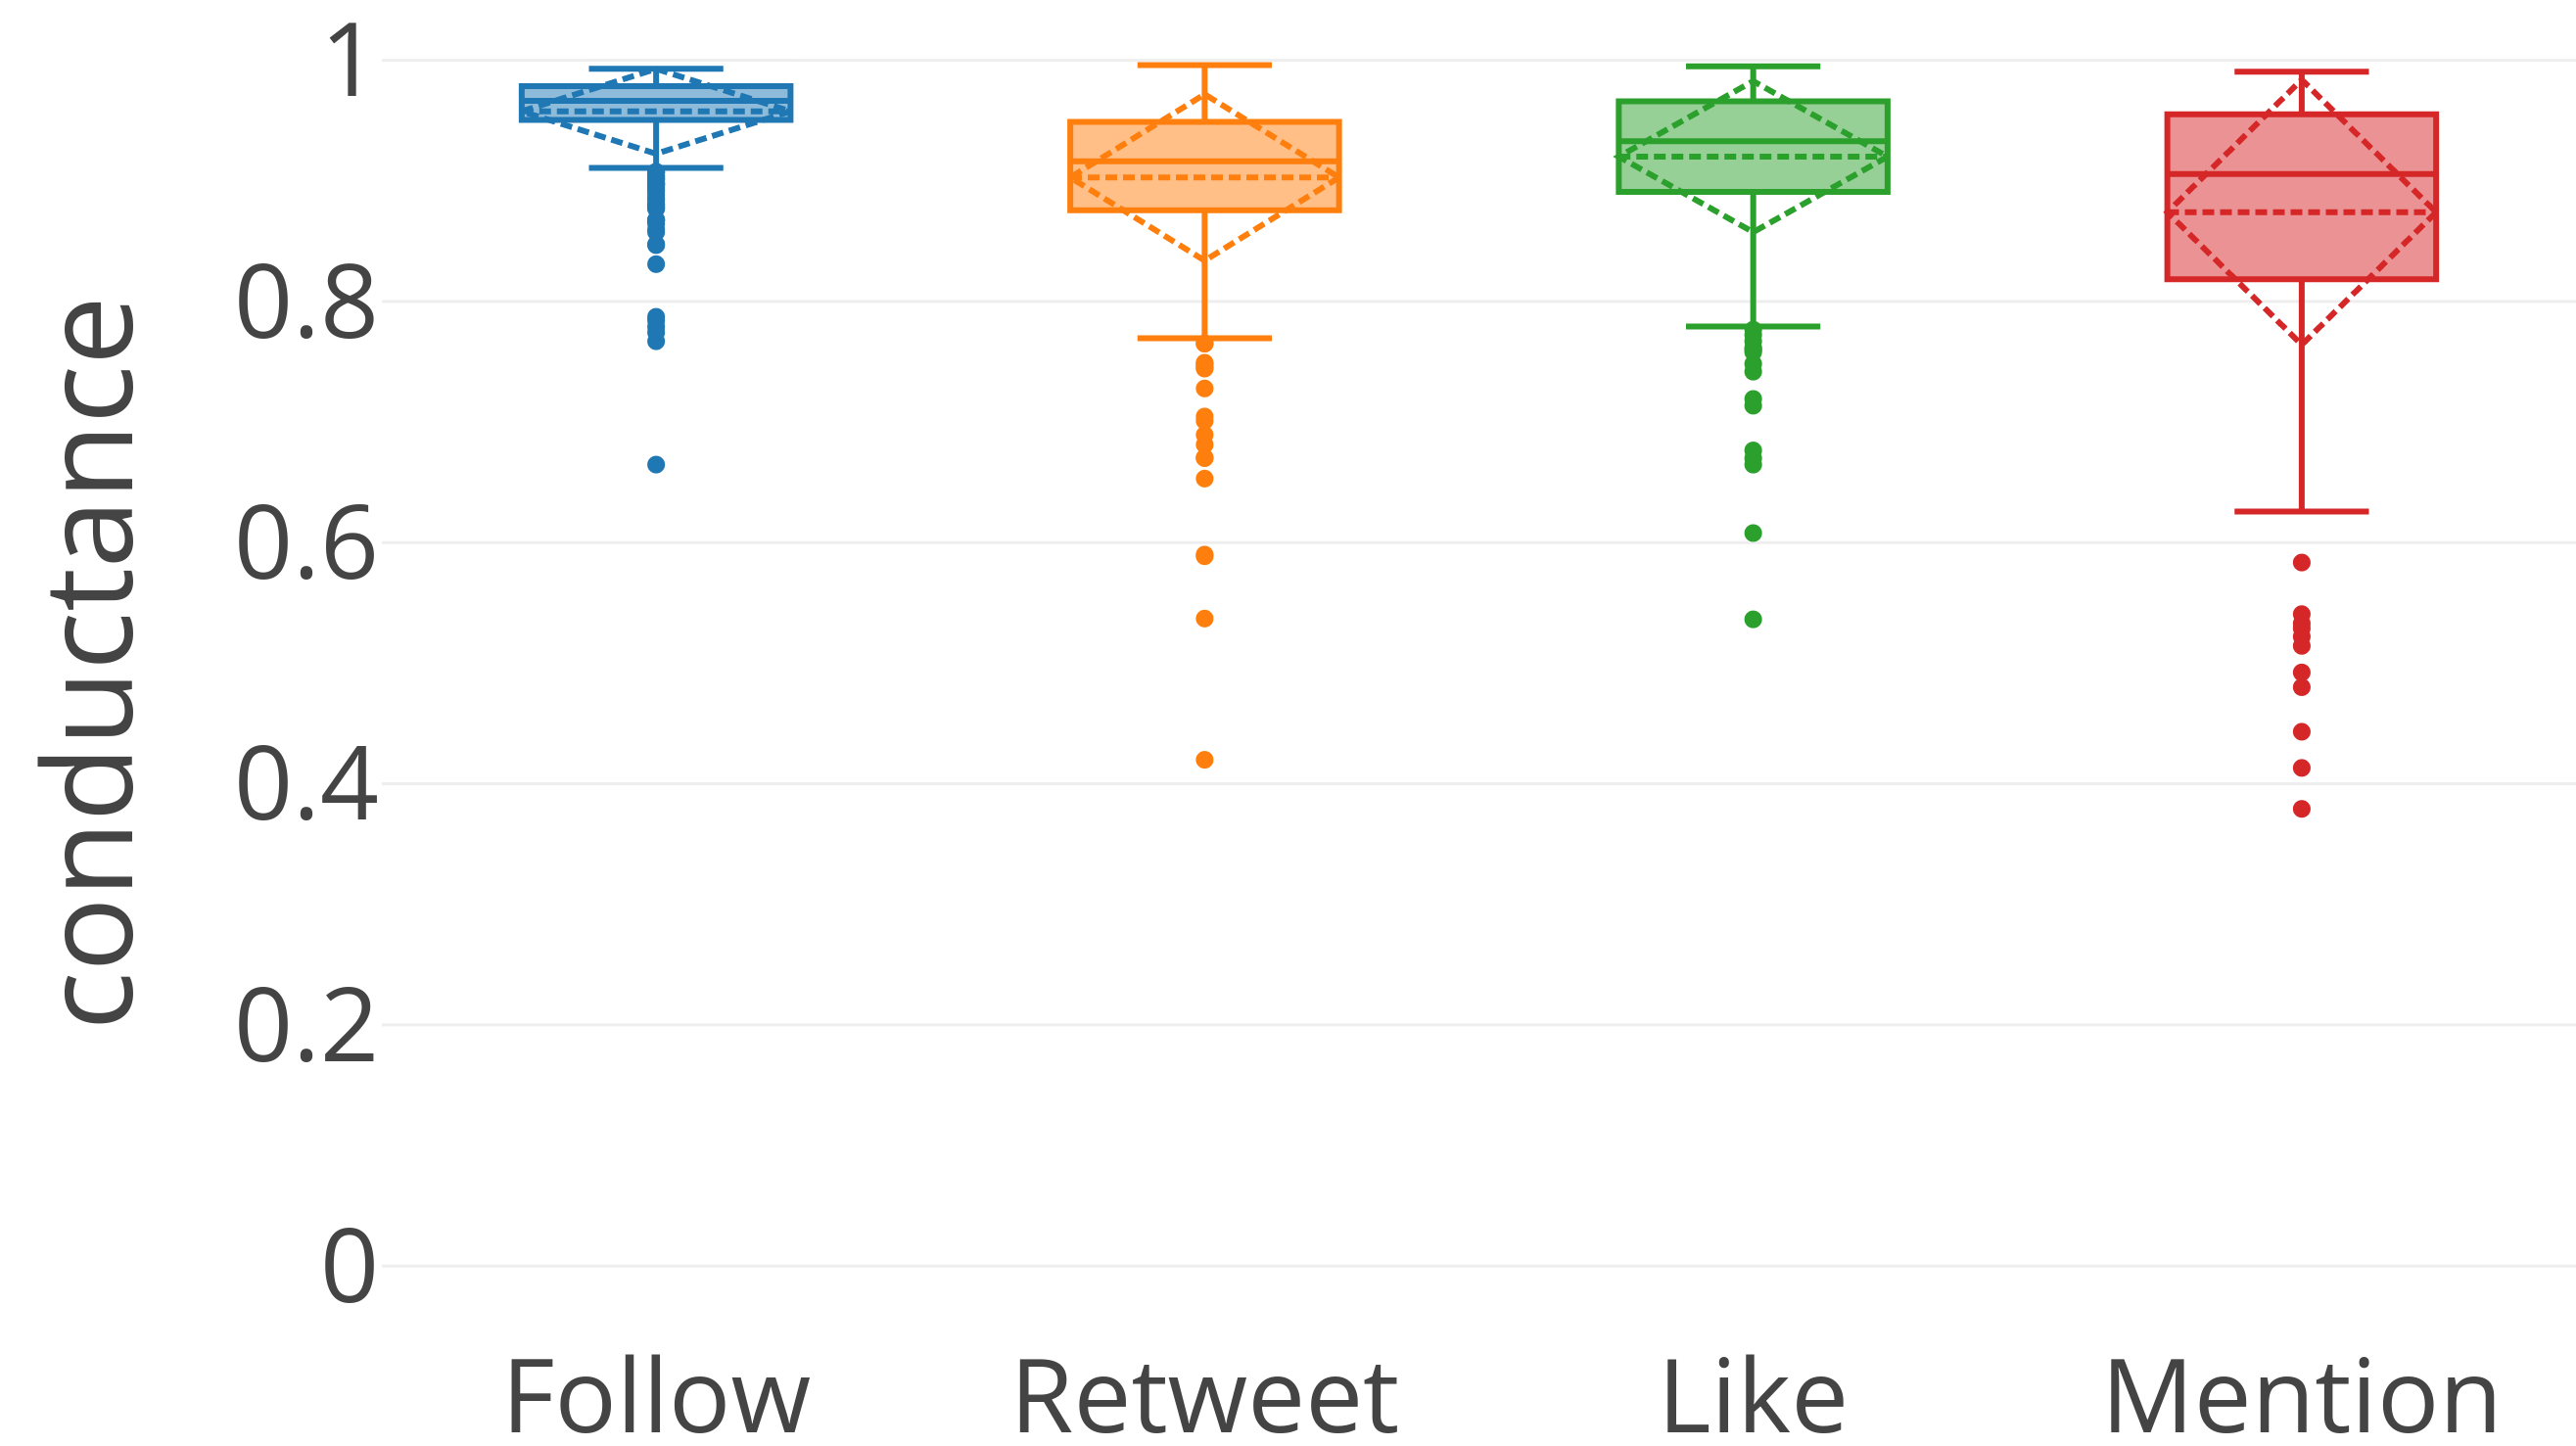
\includegraphics[width=0.47\textwidth]{fig/comm_metrics/oslom/oslom_conductance.png}
        \label{fig:comm_metrics_conductance_oslom}
    }
    \caption{Average Conductance values found in detected communities in each layer of the 500 multilayer ego networks.}
    \label{fig:comm_metrics_conductance}
\end{figure}

In order to compare the quality of communities in different layers, we evaluated the communities obtained for each ego and layer using the quality measures described in Section \ref{sec:comm_quality}. The objective of this analysis is to verify if there are significant differences as to the quality of the communities detected in each of the analyzed layers for each mulitplex ego networks, that is, is it possible that one layer produces communities with higher quality than another?



Fig. \ref{fig:comm_metrics_conductance} shows the results obtained from the calculation of the mean conductance of the communities detected by each algorithm in each ego network, according to Eq. \ref{eq:conductance}. The results show that the RAK \ref{fig:comm_metrics_conductance_rak} and COPRA \ref{fig:comm_metrics_conductance_copra} algorithms have the lowest values, which can be explained by the fact that most ego networks have a low number of communities, as shown in Fig. \ref{fig:comm_stats_avg_size_comm}. The OSLOM \ref{fig:comm_metrics_conductance_oslom} algorithm returned communities with very high conductance, indicating that communities are not isolated from each other, with many inter-community edges linking them. The algorithm INFOMAP \ref{fig:comm_metrics_conductance_infomap} brought communities with intermediate values of conductance to the communities. It may be noted that there is little difference when comparing the layers, with the mention layer having a small advantage if we consider a greater number of communities per ego network and that a good community must have low values of conductance.

\begin{figure}[h!tb]
    \centering
    \subfigure[RAK]{
        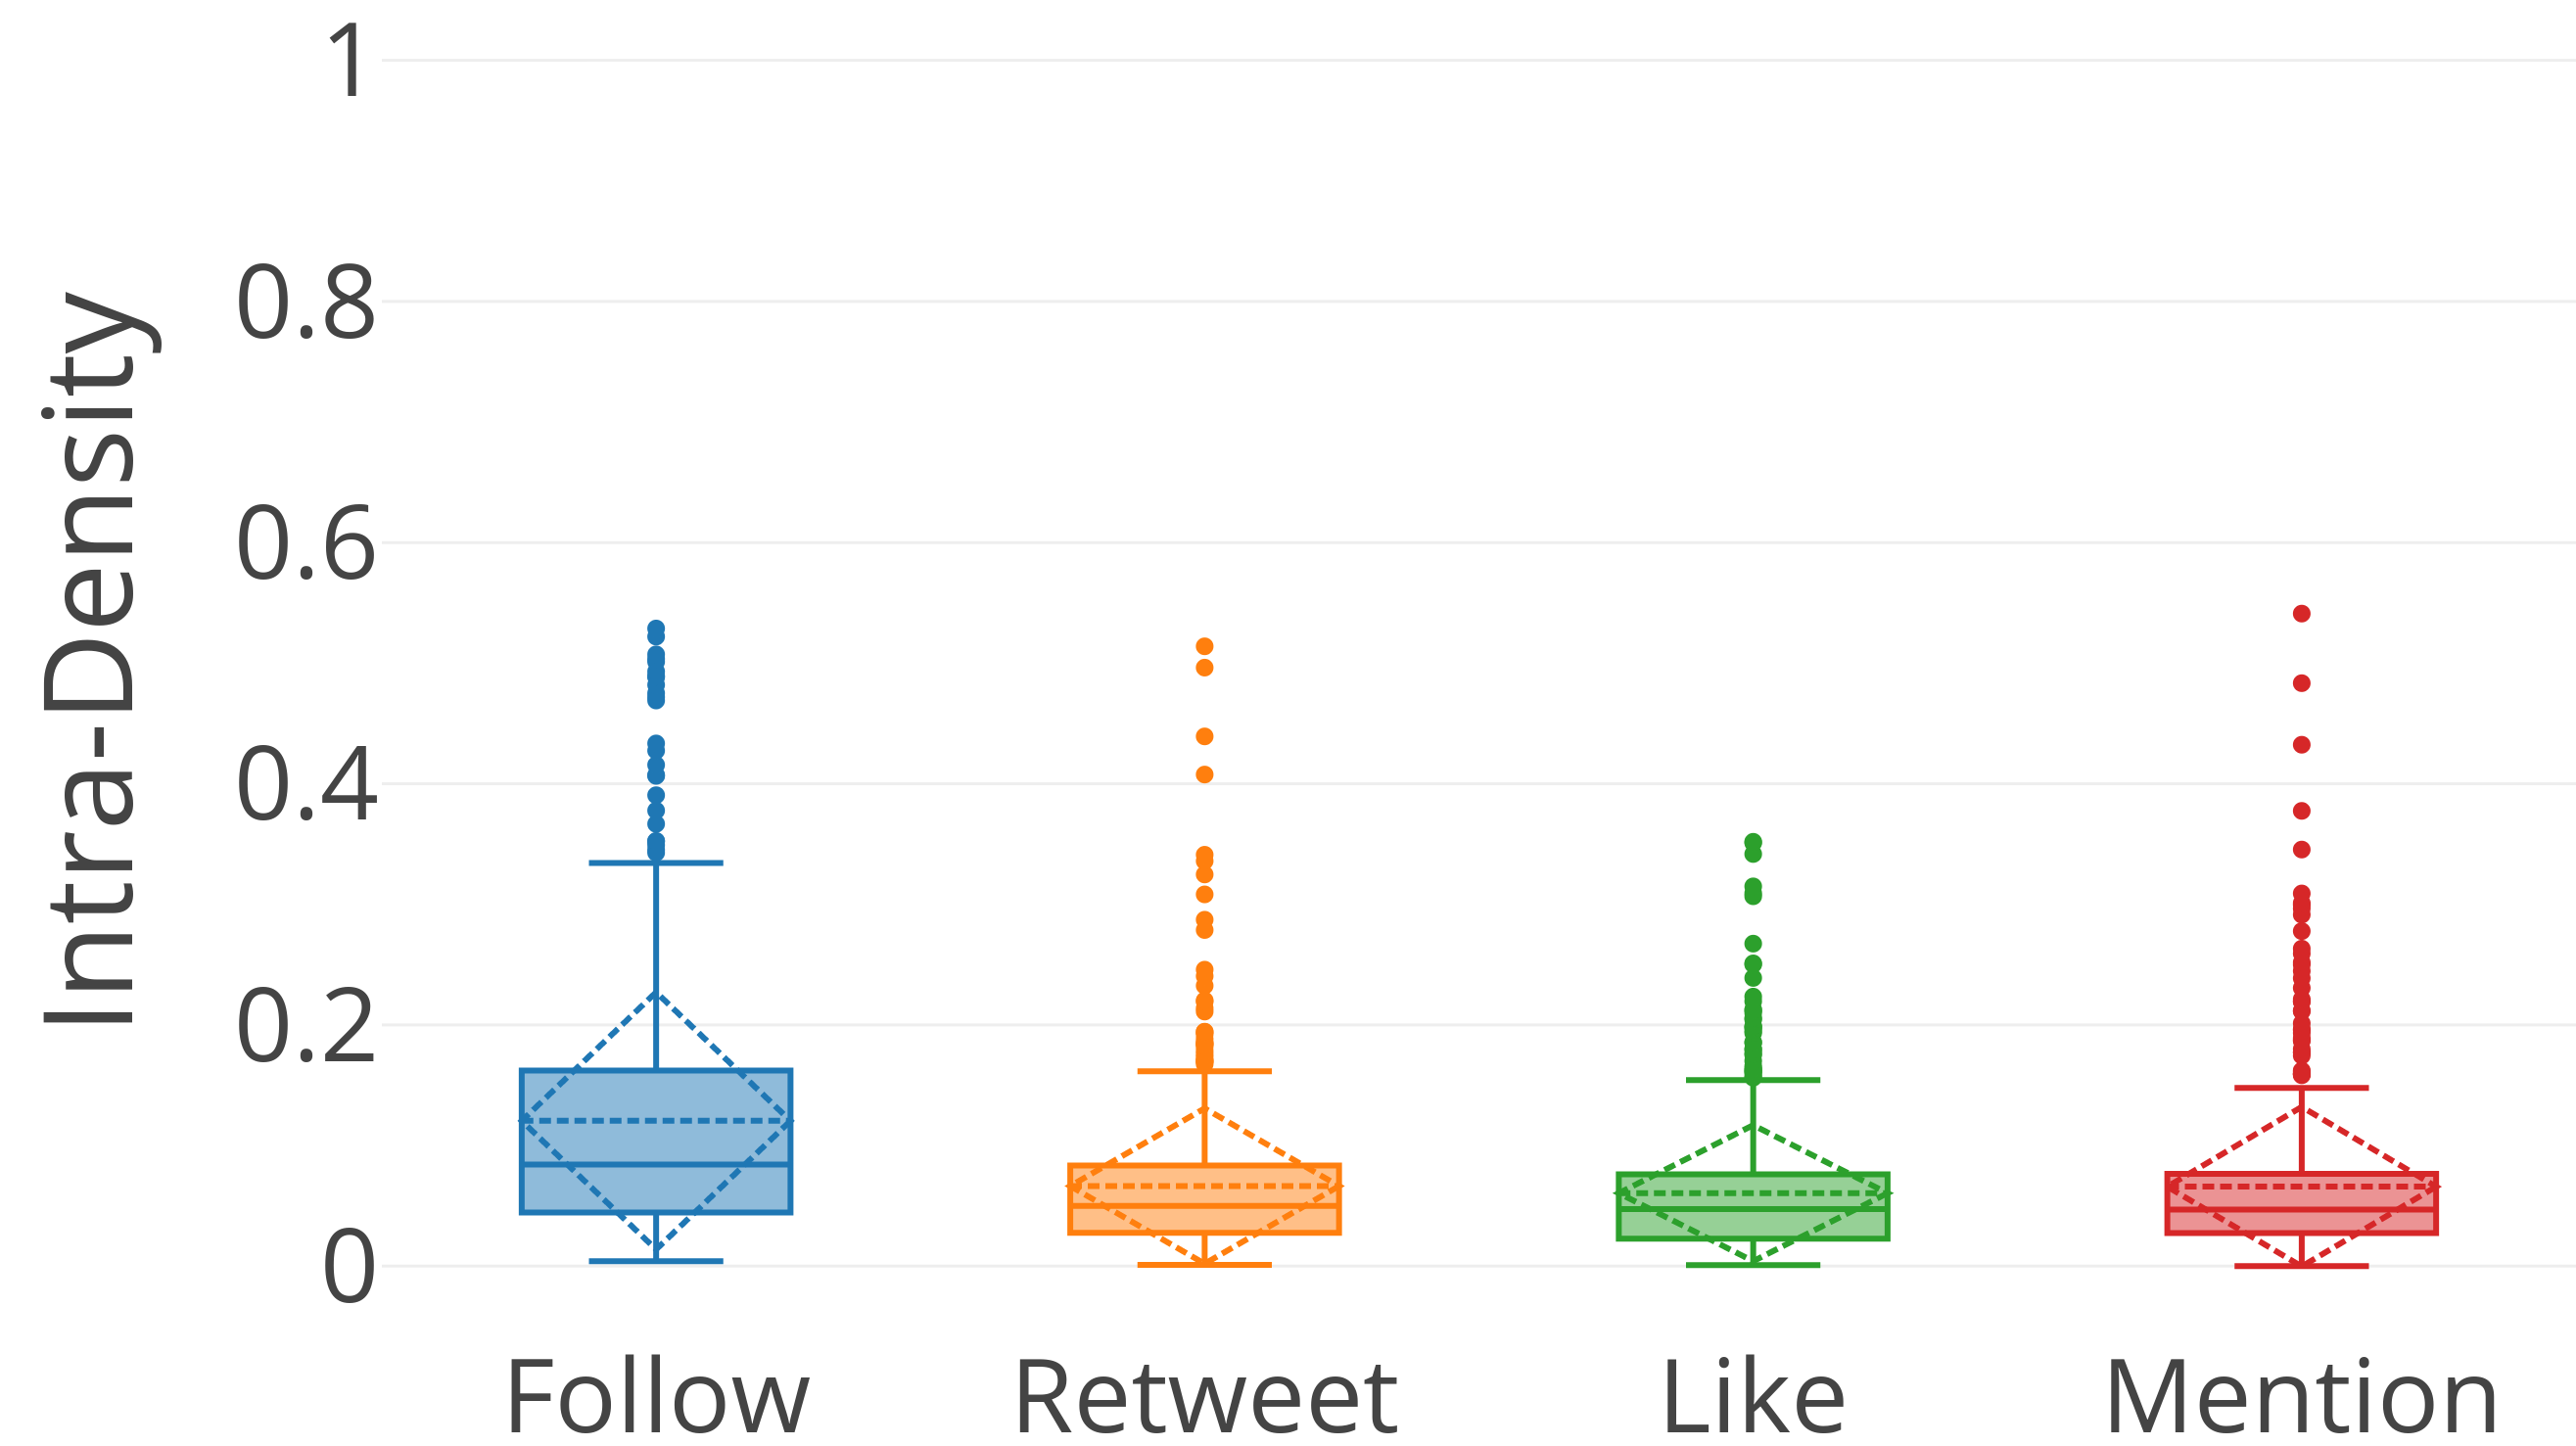
\includegraphics[width=0.47\textwidth]{fig/comm_metrics/rak/rak_intra_density.png}
        \label{fig:comm_metrics_intra_density_rak}
    }
    \subfigure[INFOMAP]{
        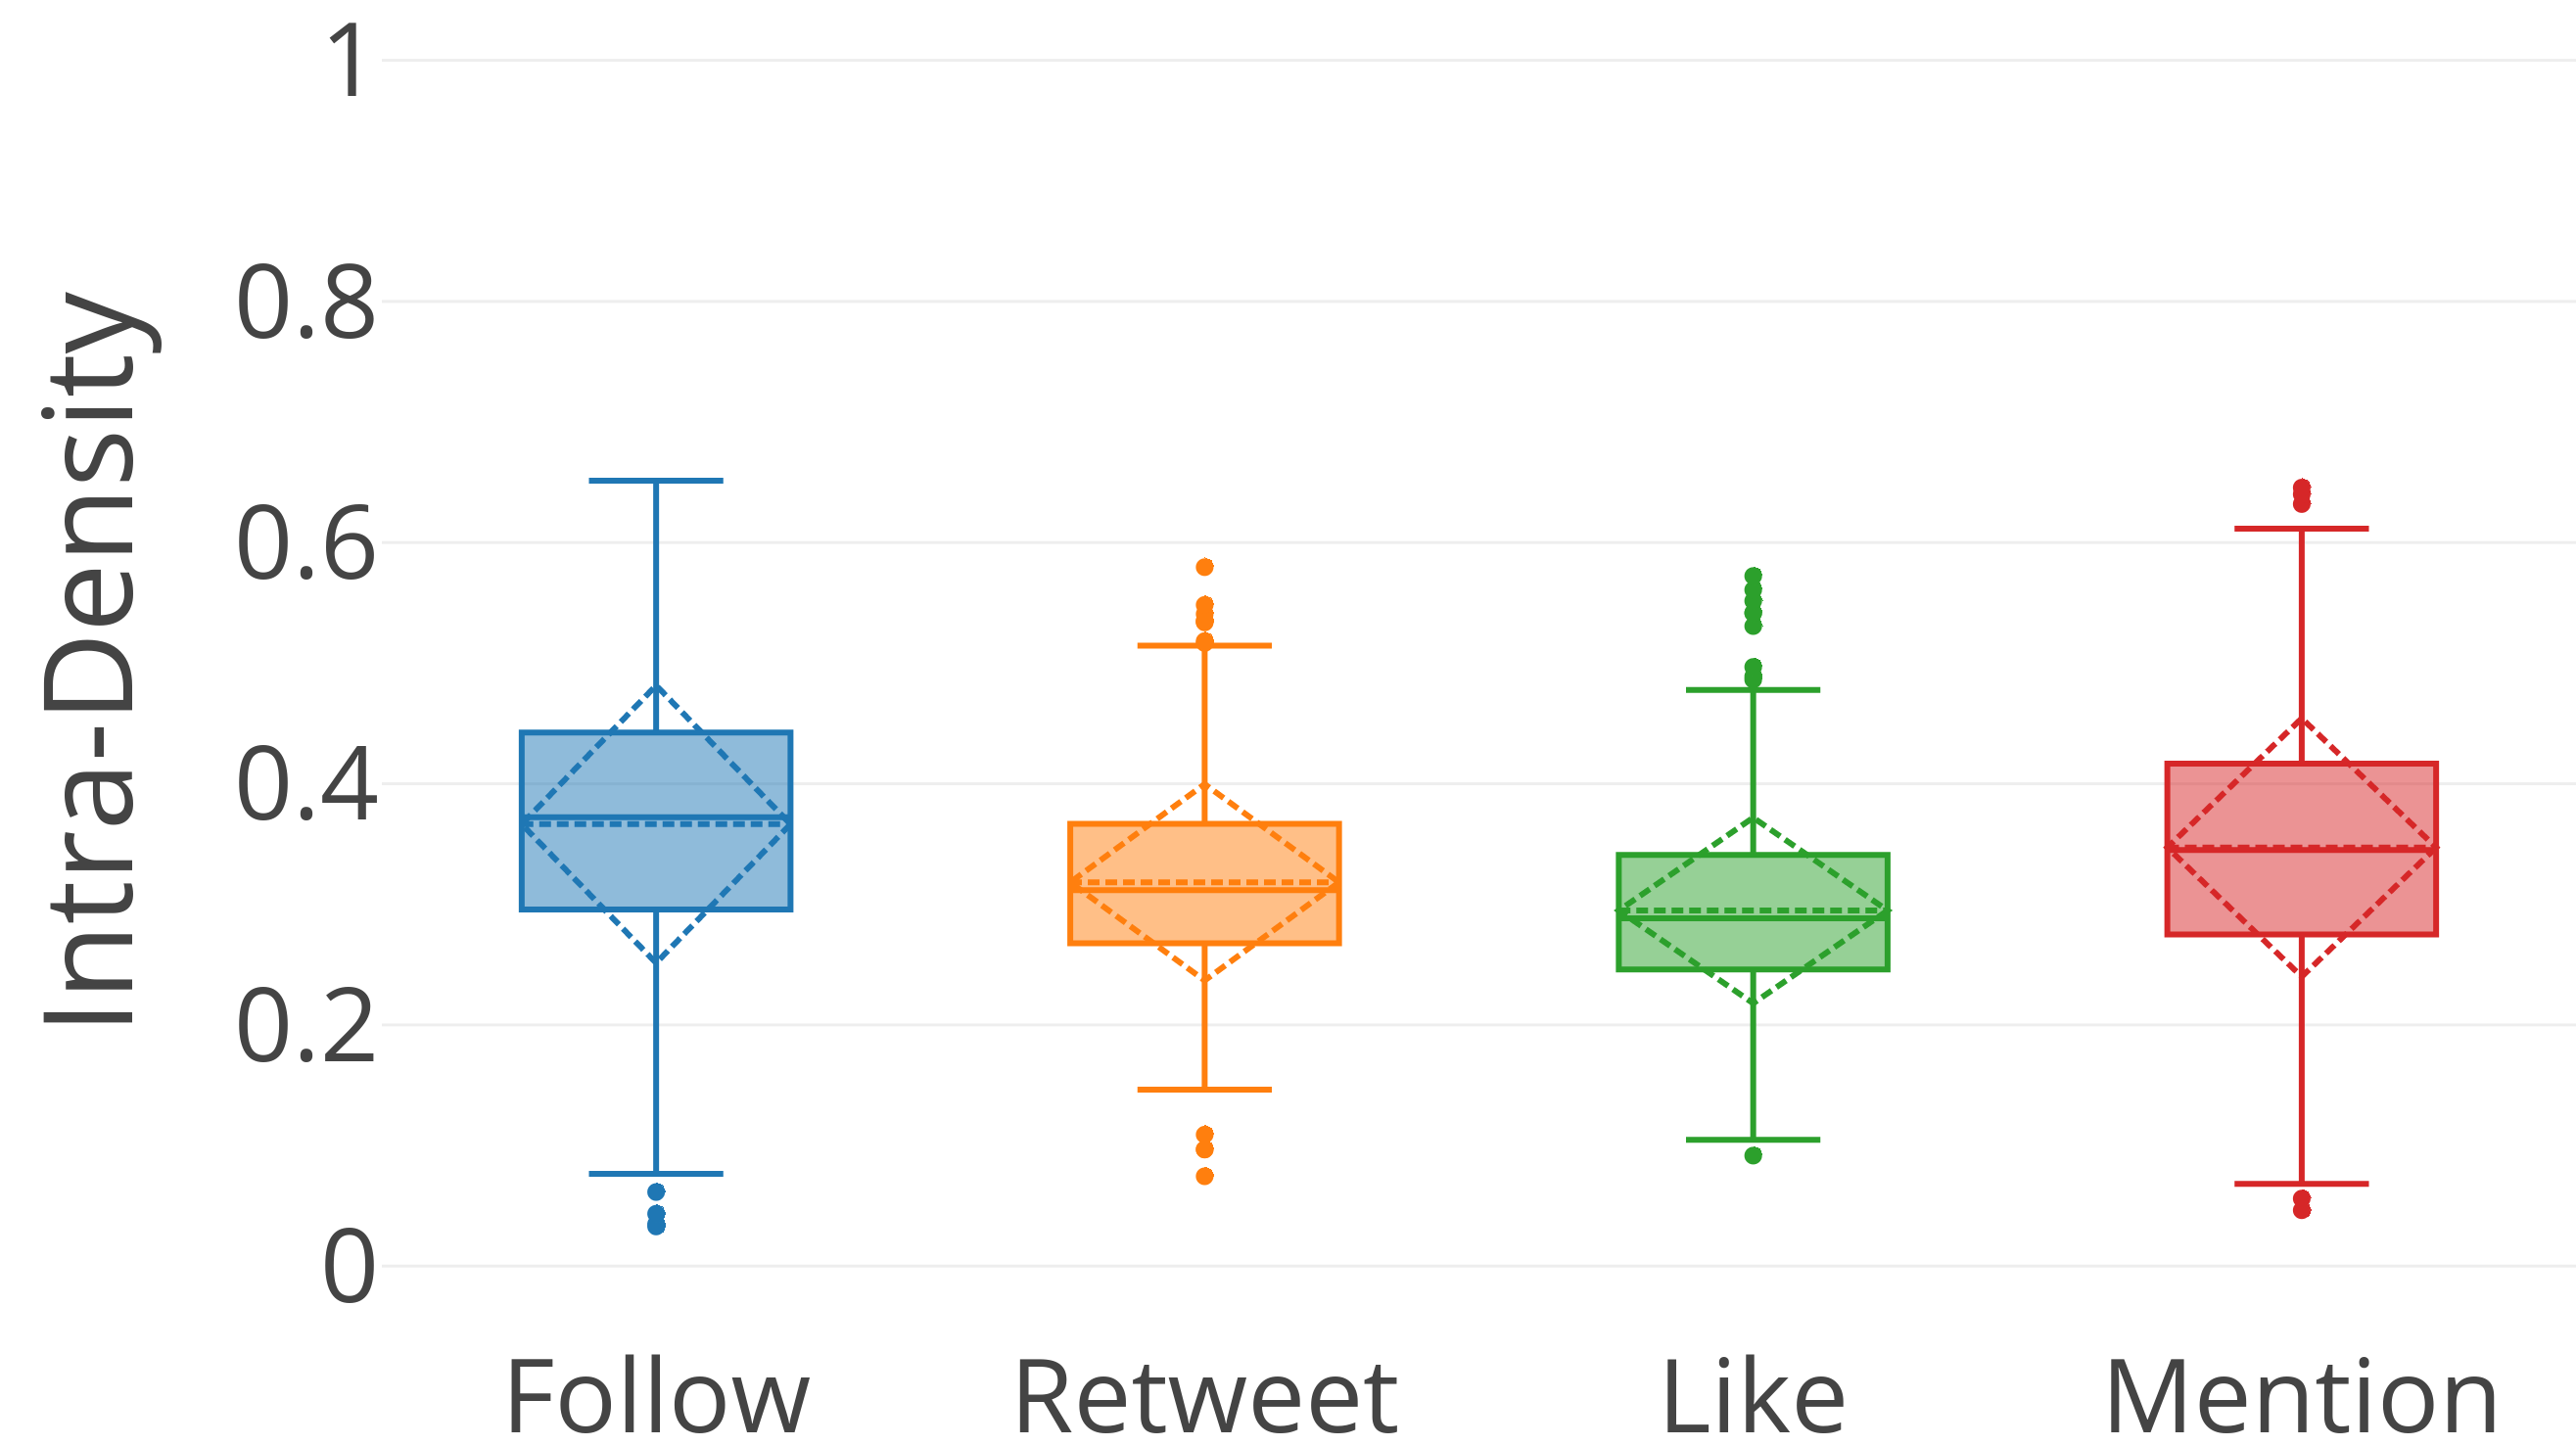
\includegraphics[width=0.47\textwidth]{fig/comm_metrics/infomap/infomap_intra_density.png}
        \label{fig:comm_metrics_intra_density_infomap}
    } \\
    \subfigure[COPRA]{
        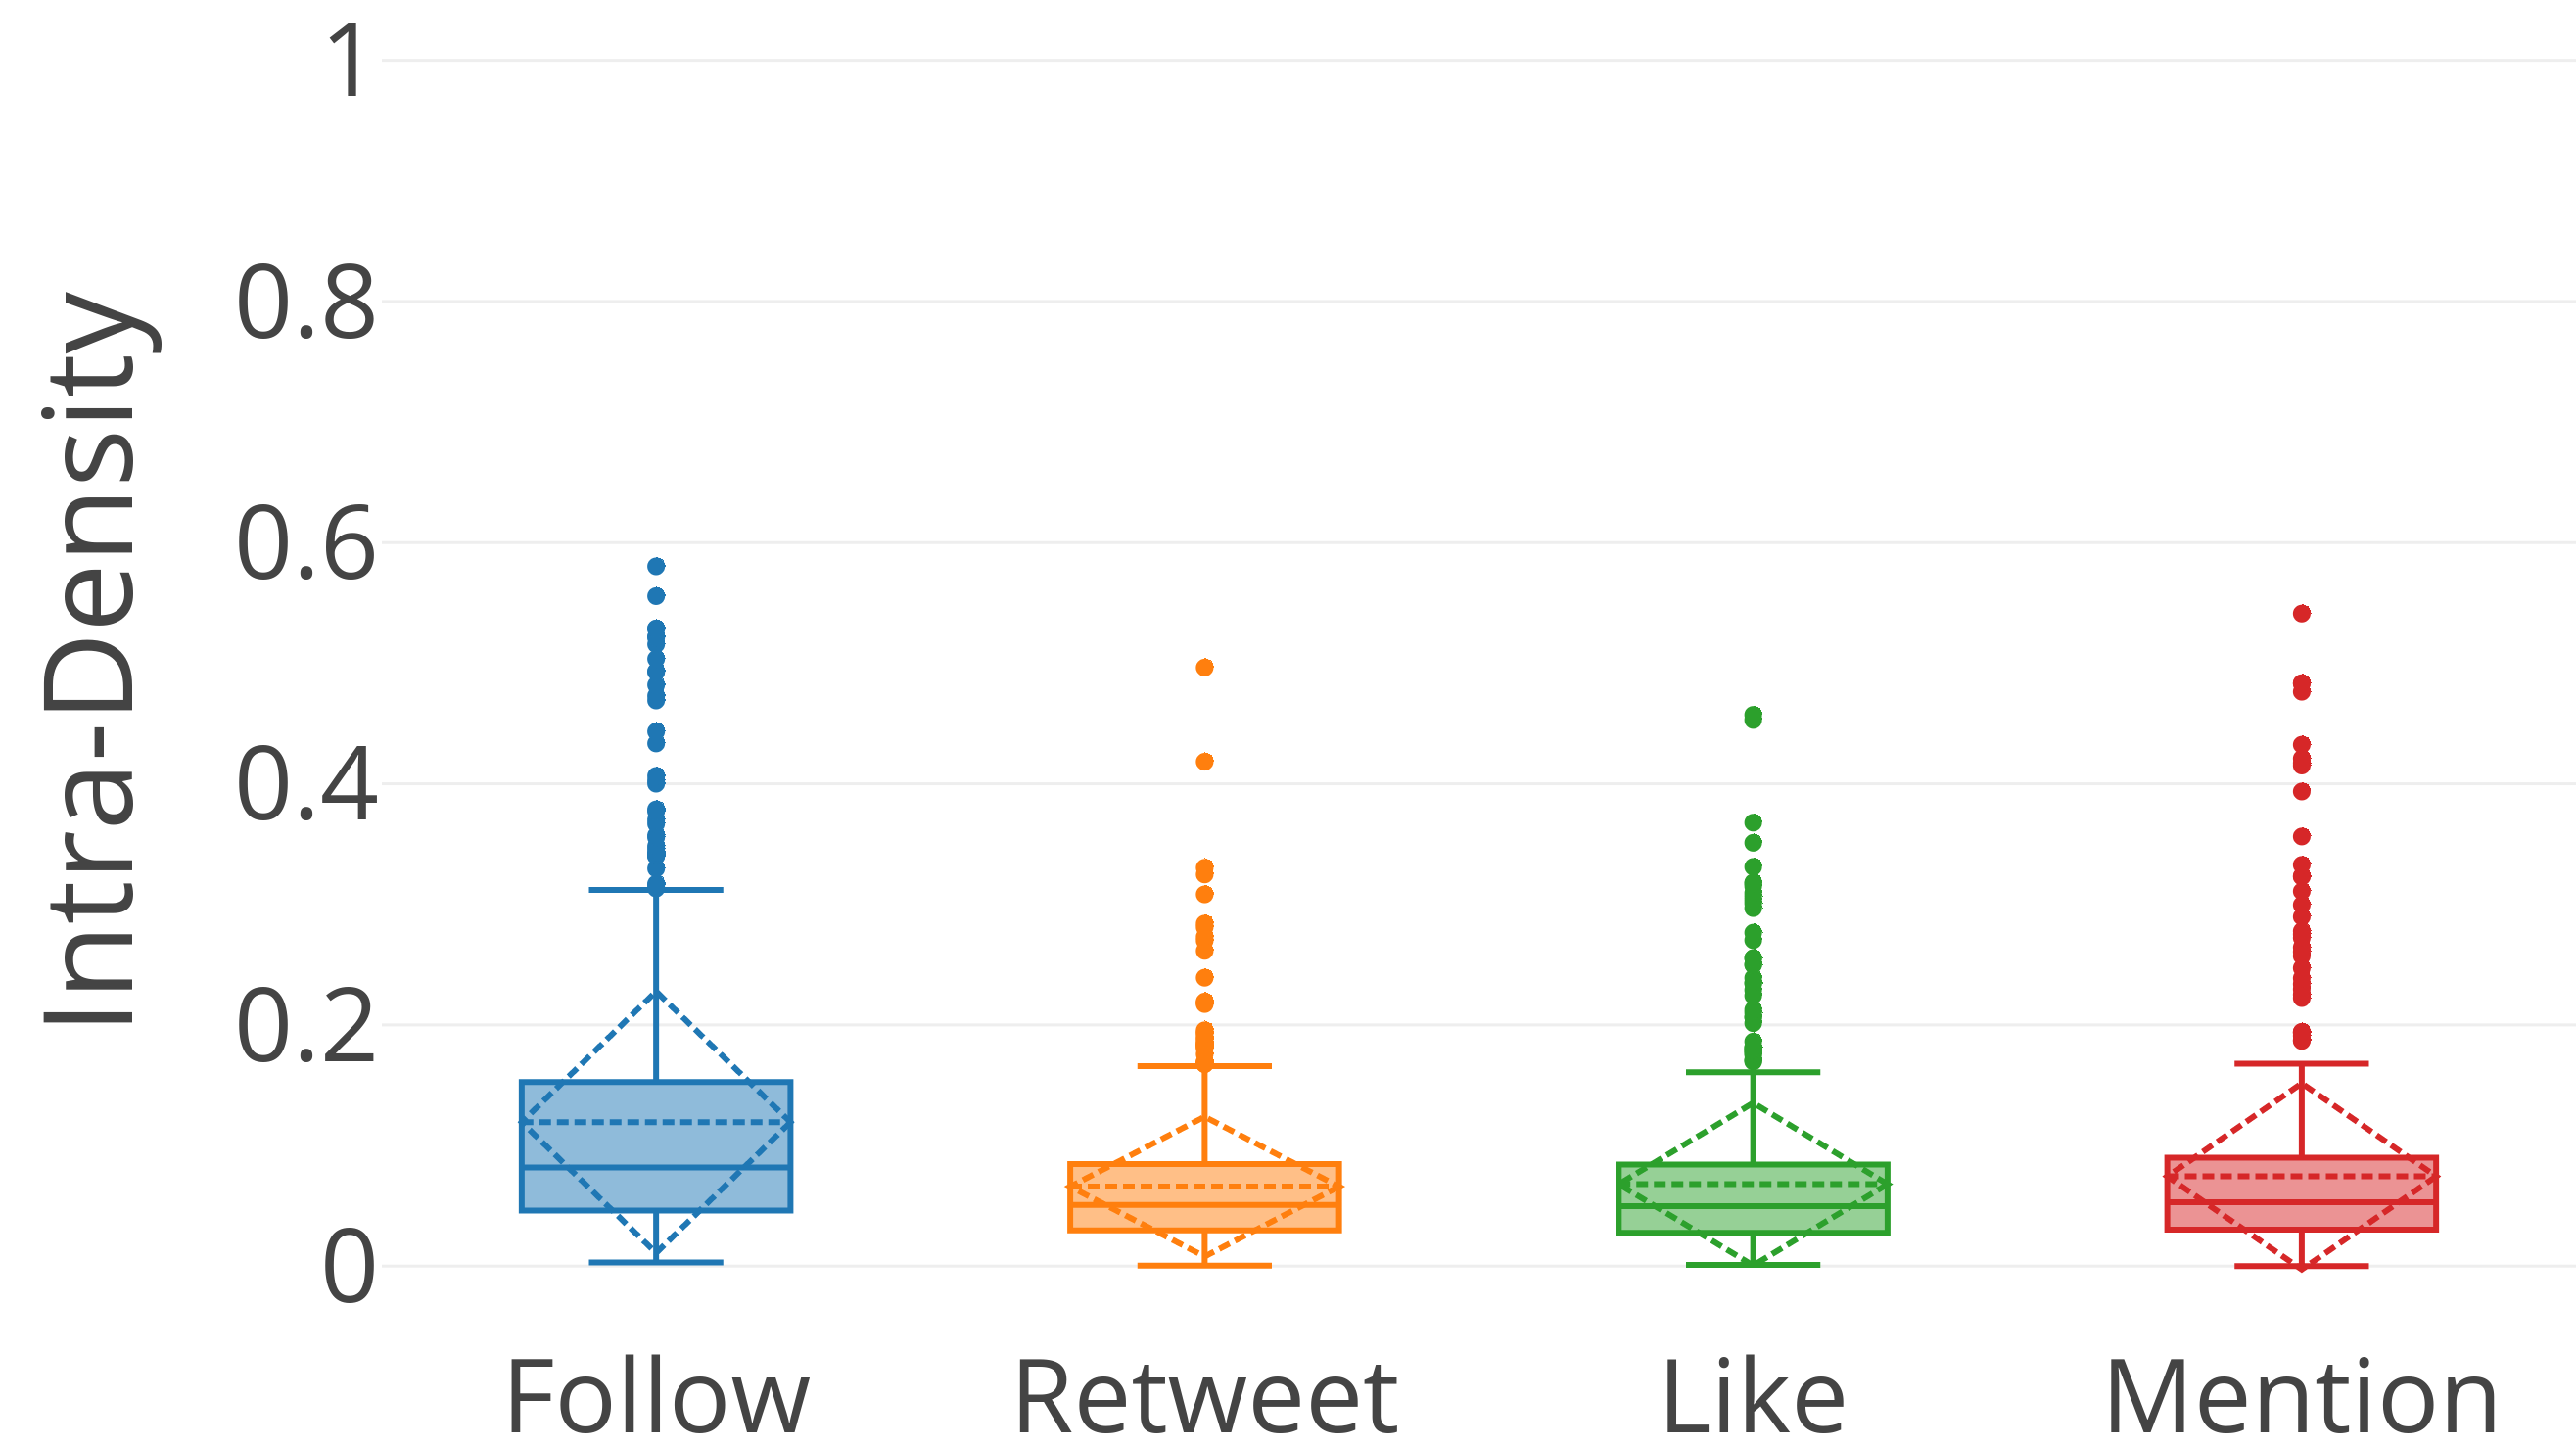
\includegraphics[width=0.47\textwidth]{fig/comm_metrics/copra/copra_intra_density.png}
        \label{fig:comm_metrics_intra_density_copra}
    }
    \subfigure[OSLOM]{
        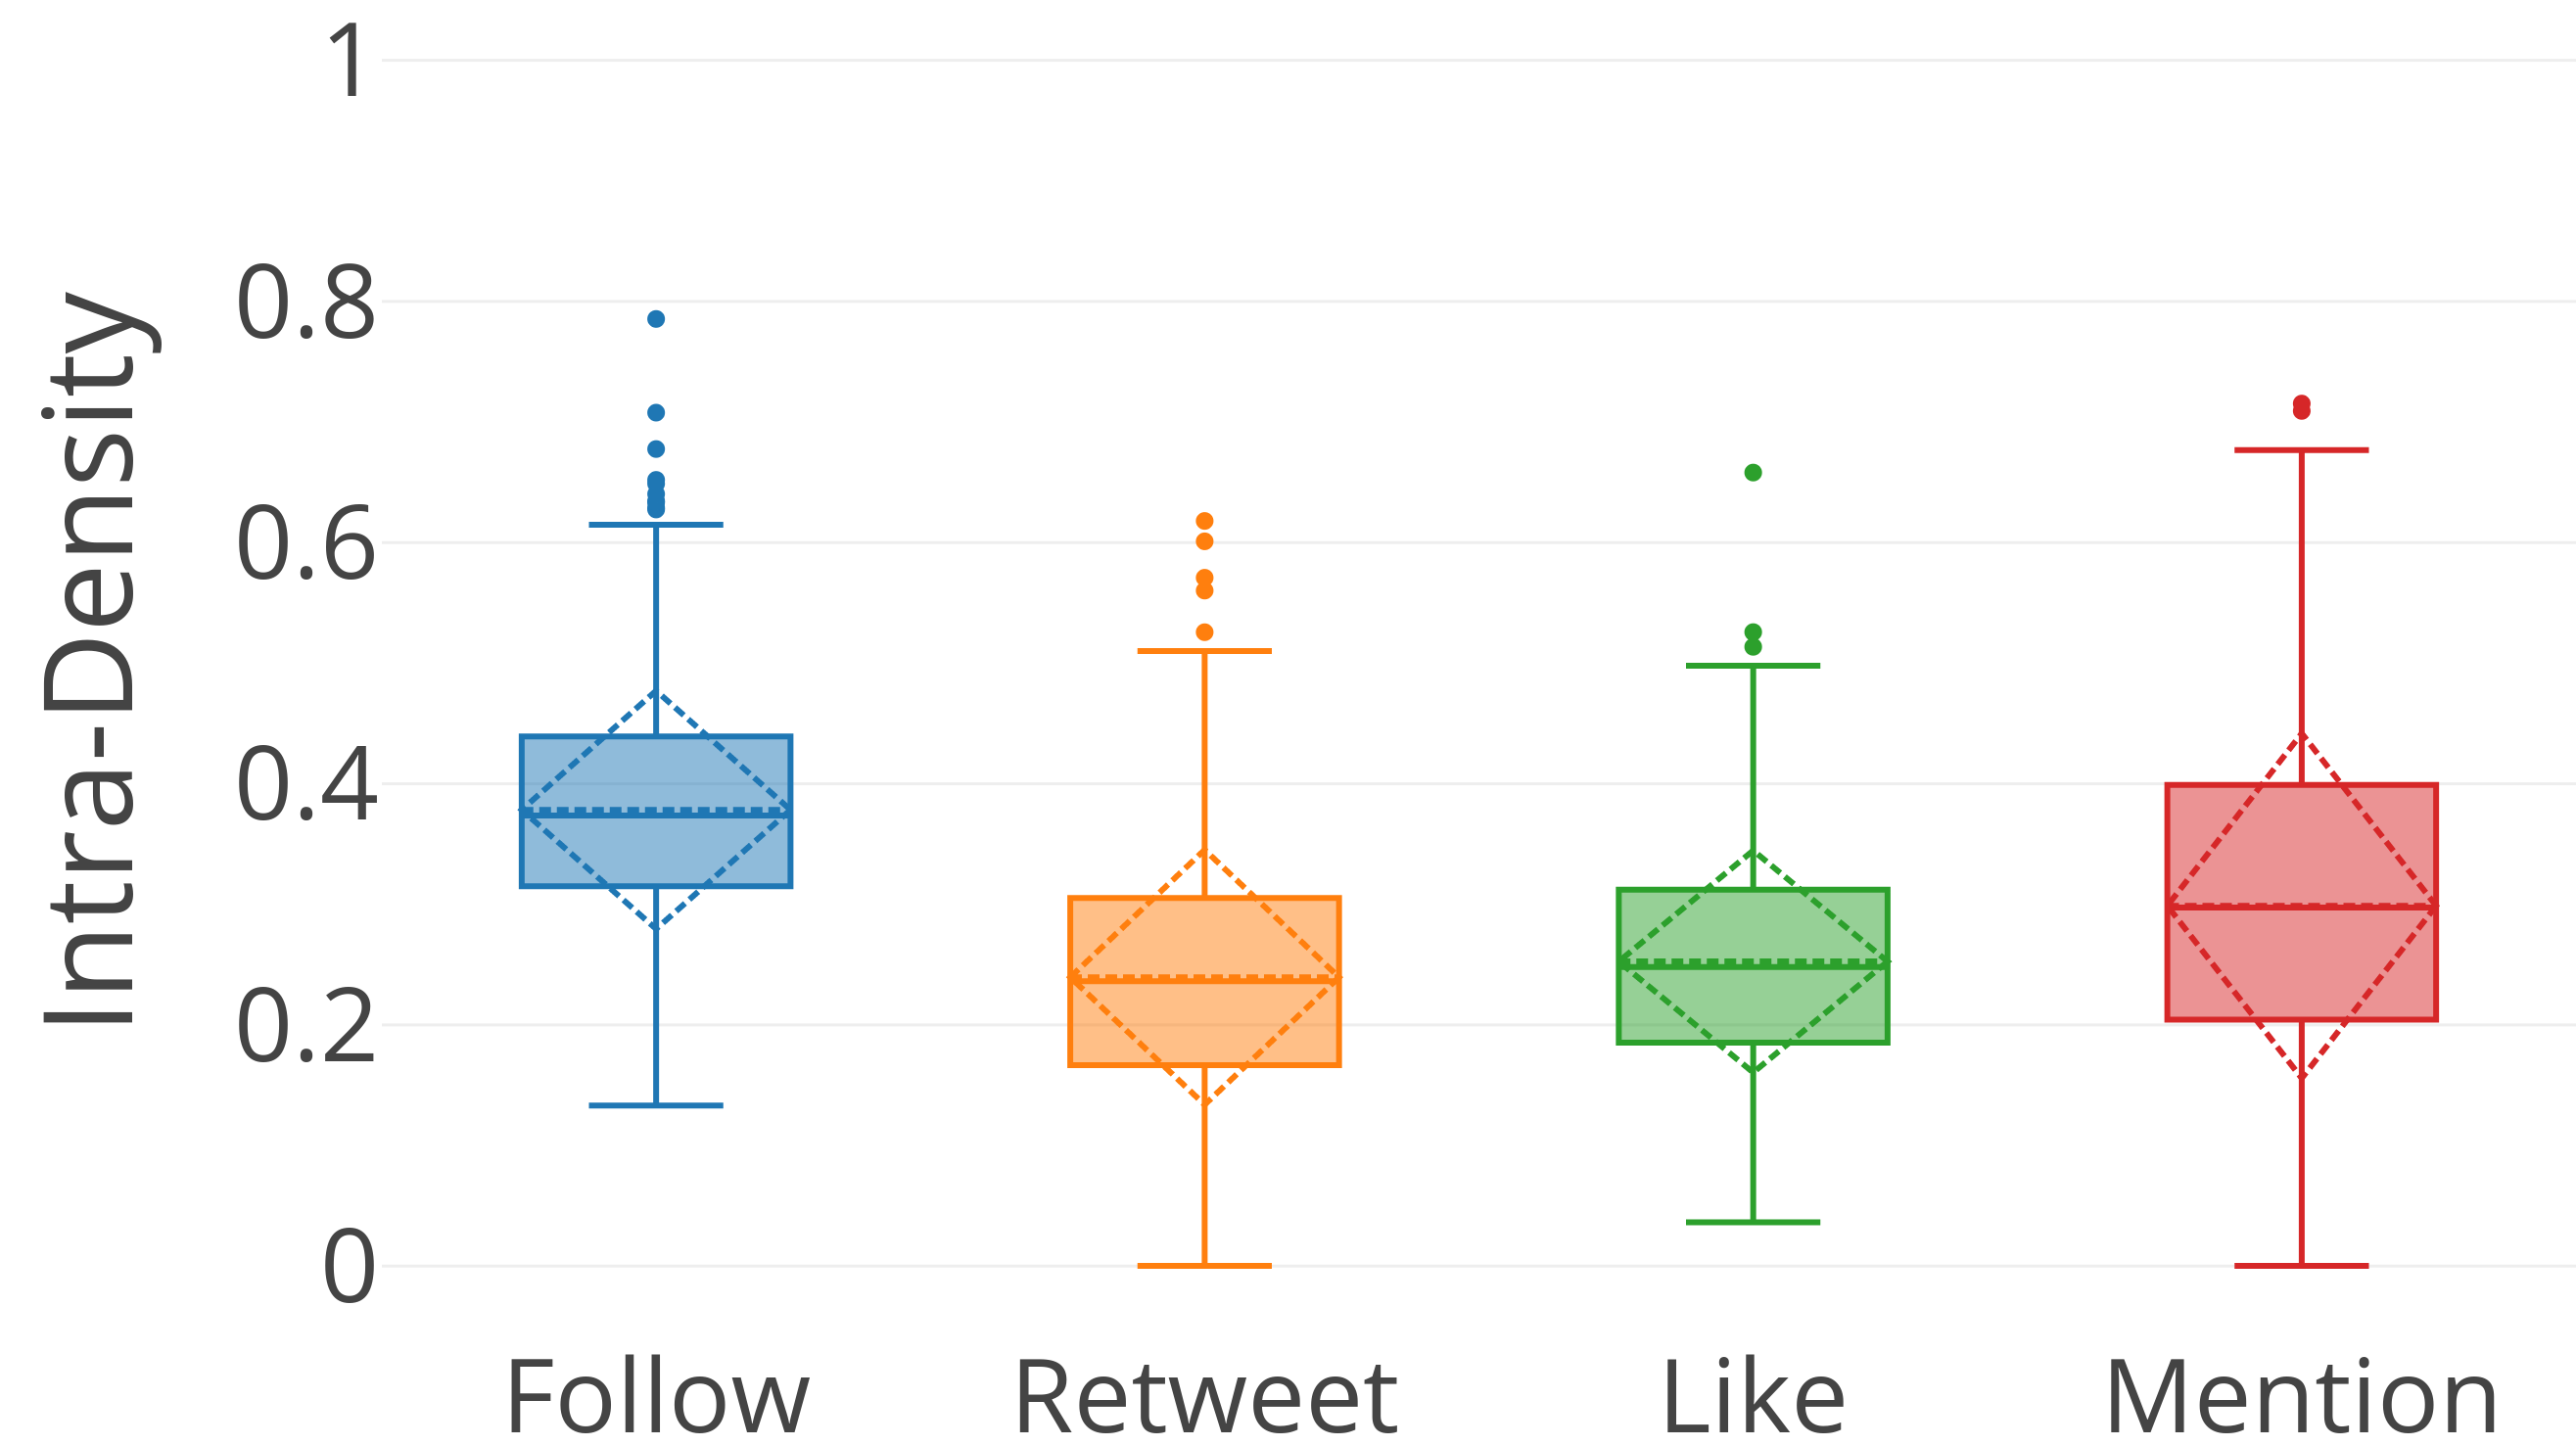
\includegraphics[width=0.47\textwidth]{fig/comm_metrics/oslom/oslom_intra_density.png}
        \label{fig:comm_metrics_intra_density_oslom}
    }
    \caption{Average Internal Density values found in detected communities in each layer of the 500 multilayer ego networks.}
    \label{fig:comm_metrics_intra_density}
\end{figure}


\begin{figure}[h!tb]
    \centering
    \subfigure[RAK]{       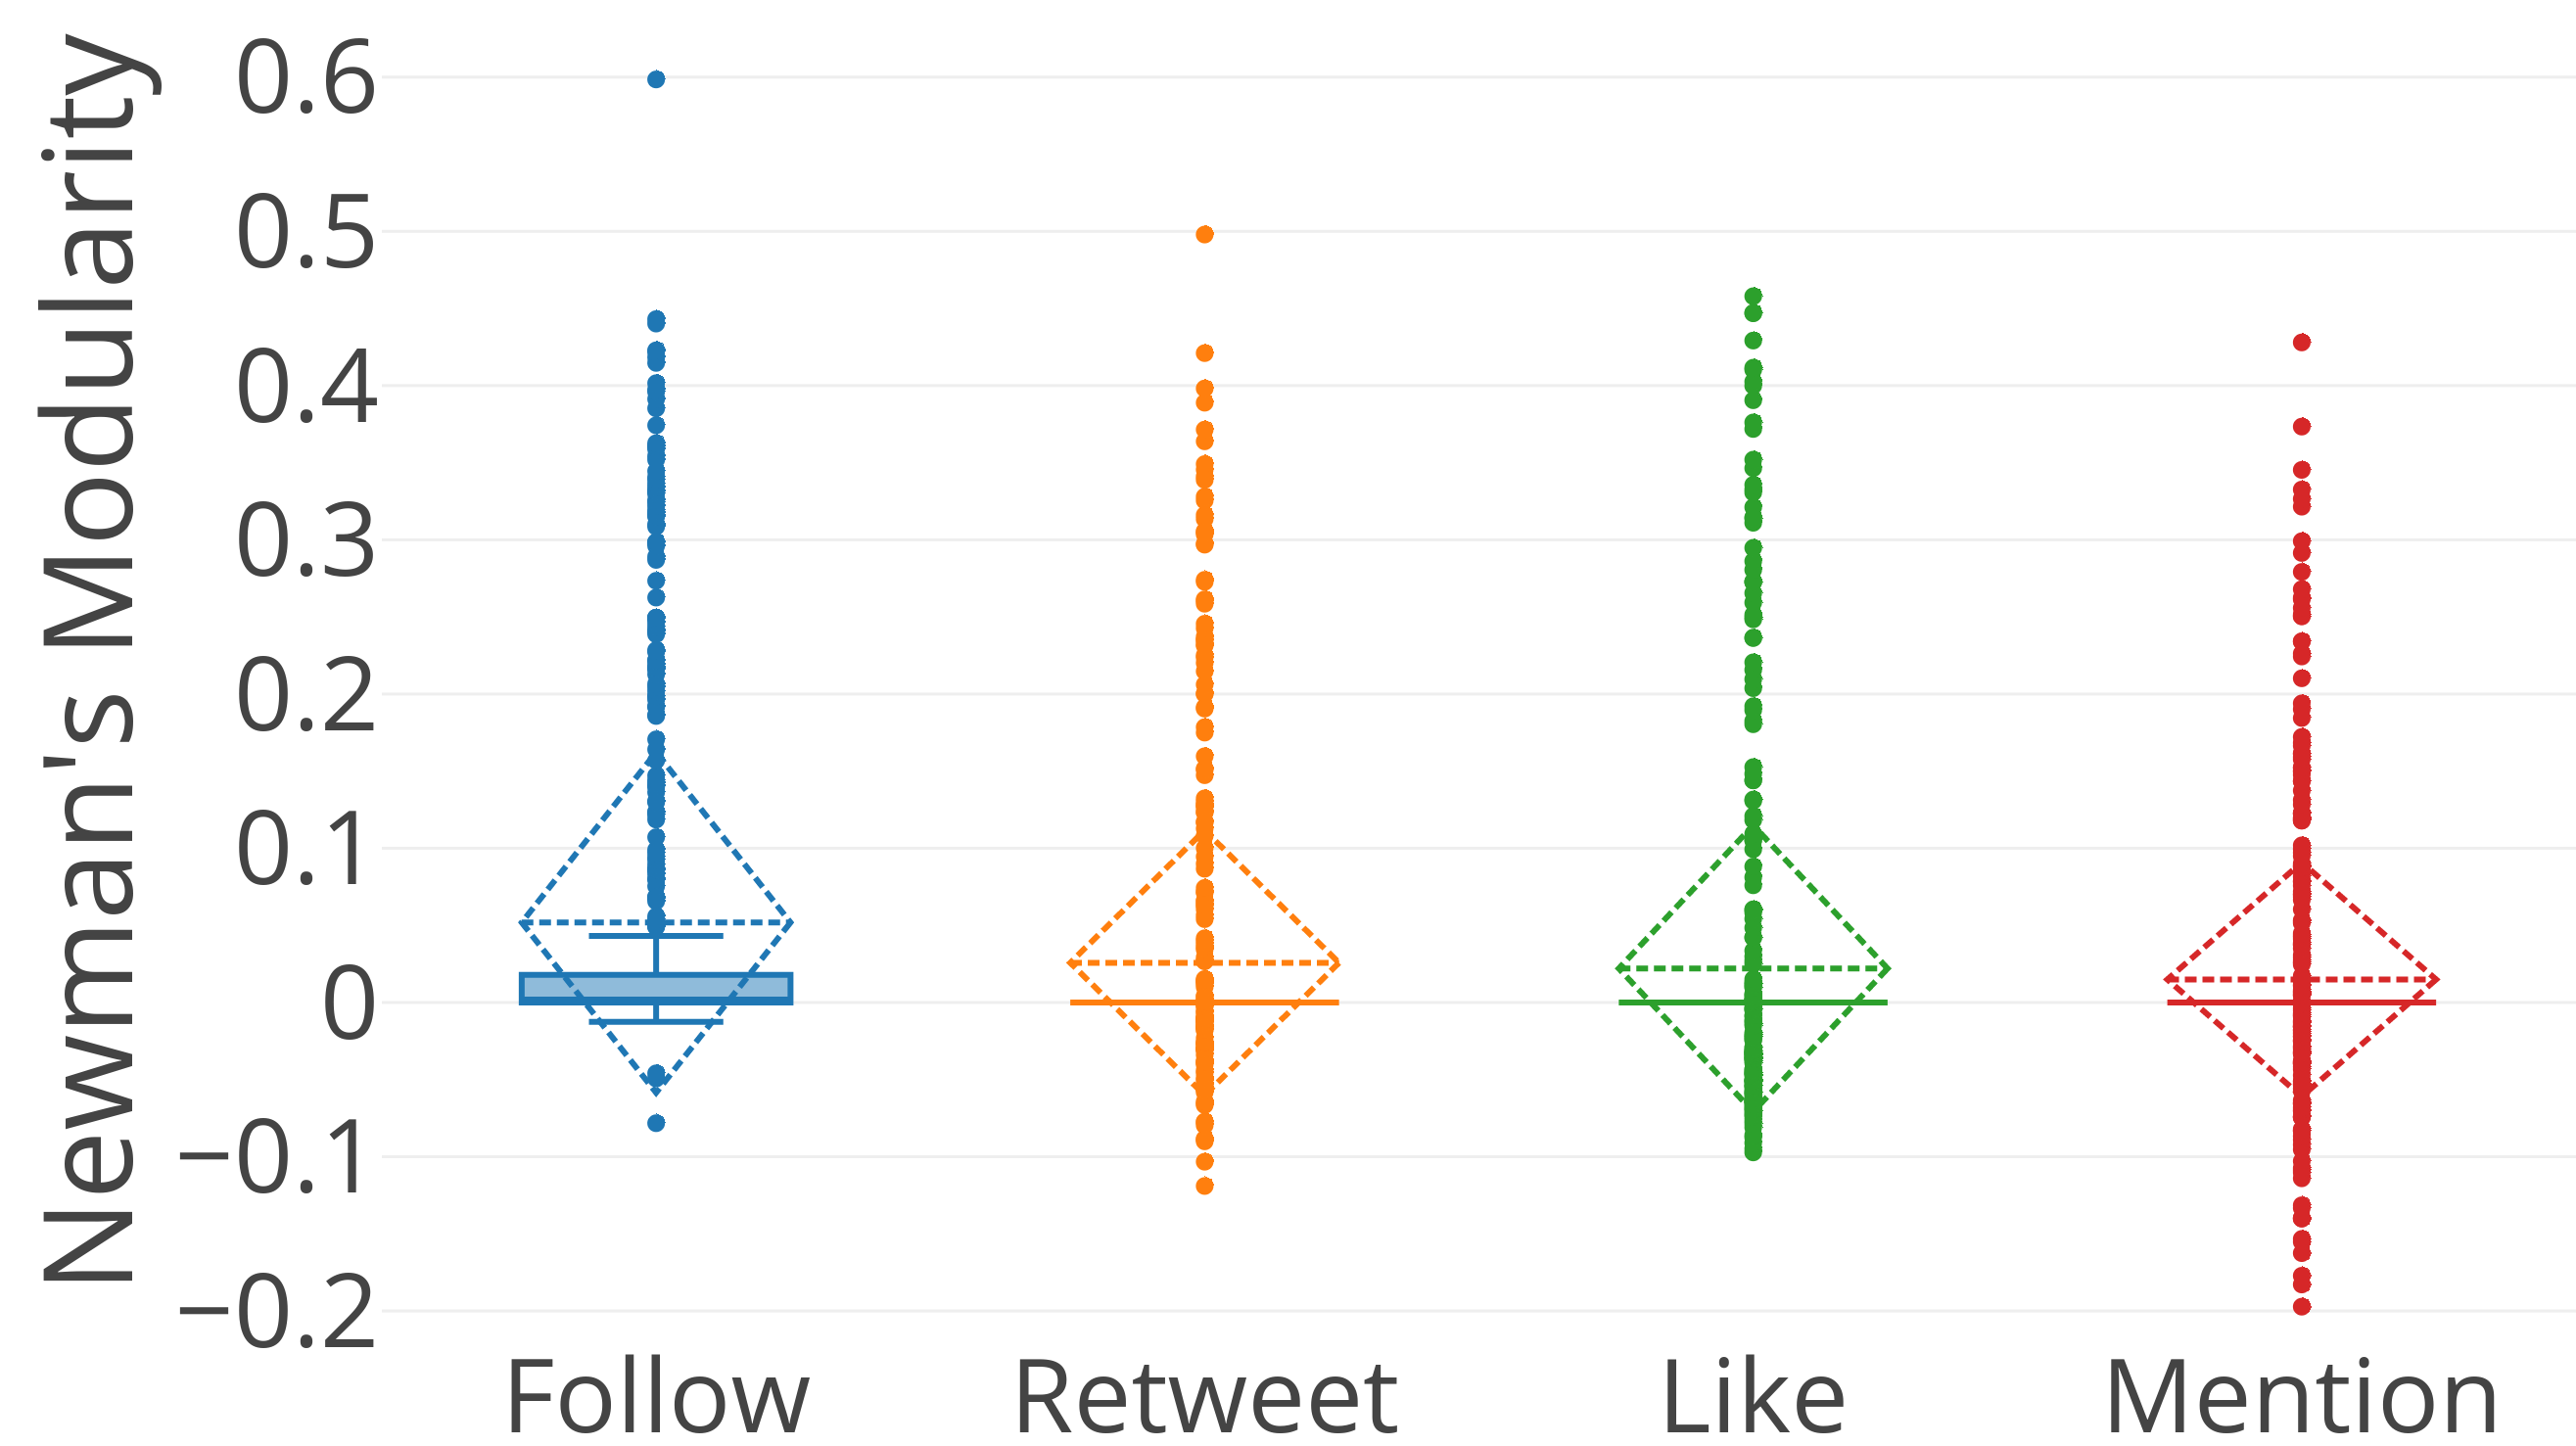
\includegraphics[width=0.47\textwidth]{fig/comm_metrics/rak/rak_modularity.png}        \label{fig:comm_metrics_modularity_rak}
    }
    \subfigure[INFOMAP]{
        \includegraphics[width=0.47\textwidth]{fig/comm_metrics/infomap/infomap_modularity.png}
        \label{fig:comm_metrics_modularity_infomap}
    } \\
    \subfigure[COPRA]{
        \includegraphics[width=0.47\textwidth]{fig/comm_metrics/copra/copra_modularity.png}
        \label{fig:comm_metrics_modularity_copra}
    }
    \subfigure[OSLOM]{
        \includegraphics[width=0.47\textwidth]{fig/comm_metrics/oslom/oslom_modularity.png}
        \label{fig:comm_metrics_modularity_oslom}
    }
    \caption{Average Newman{'}s Modularity values found in detected communities in each layer of the 500 multilayer ego networks.}
    \label{fig:comm_metrics_modularity}
\end{figure}

The Internal density of each community was also calculated, according to Eq. \ref{eq:intDensity} and the mean for each of the 500 ego networks can be found in Fig. \ref{fig:comm_metrics_intra_density}. When we compare these results of the internal density of communities with the density of the layers, observed in Fig. \ref{fig:net_struct_density} the values presented by the RAK \ref{fig:comm_metrics_intra_density_rak} and COPRA \ref{fig:comm_metrics_intra_density_copra} algorithms are practically the same found for the density of the entire layer, which reinforces the conclusion that these algorithms detected few or only a community composed of almost all vertices of the ego network. For the INFOMAP \ref{fig:comm_metrics_intra_density_infomap} and OSLOM \ref{fig:comm_metrics_intra_density_oslom} algorithms, the density of the detected communities is much higher than the whole layer density (about one order of magnitude), showing  that all the layers considered show relevant community structure.


The values of Newman's Modularity are shown in Fig. \ref{fig:comm_metrics_modularity}. The calculation of this metric was performed according to Eq. \ref{eq:newmanModularity}. The presentation of the results follows the same procedure adopted for conductance and internal density. The quality of the communities detected by the INFOMAP algorithm is greater than the communities detected by the other algorithms, according to Newman's modularity, as we can see in Fig. \ref{fig:comm_metrics_modularity_infomap} . Again it is not possible to say that one layer stands out from the others. All results fall into the same range of values for all algorithms.

\begin{figure}[h!tb]
    \centering
    \subfigure[RAK]{
        \includegraphics[width=0.47\textwidth]{fig/comm_metrics/rak/rak_mod_density.png}
        \label{fig:comm_metrics_mod_density_rak}
    }
    \subfigure[INFOMAP]{
        \includegraphics[width=0.47\textwidth]{fig/comm_metrics/infomap/infomap_mod_density.png}
        \label{fig:comm_metrics_mod_density_infomap}
    } \\
    \subfigure[COPRA]{
        \includegraphics[width=0.47\textwidth]{fig/comm_metrics/copra/copra_mod_density.png}
        \label{fig:comm_metrics_mod_density_copra}
    }
    \subfigure[OSLOM]{
        \includegraphics[width=0.47\textwidth]{fig/comm_metrics/oslom/oslom_mod_density.png}
        \label{fig:comm_metrics_mod_density_oslom}
    }
    \caption{Average Modularity-Density values found in detected communities in each layer of the 500 multilayer ego networks.}
    \label{fig:comm_metrics_mod_density}
\end{figure}


We also calculate the Modularity-Density according to Eq. \ref{eq:modDensity}, and the result is shown in Fig. \ref{fig:comm_metrics_mod_density}, where the mean Modularity-Density values are displayed for each ego network with a boxplot for each layer. The OSLOM algorithm presents the worst performance for this metric, as we can see in Fig. \ref{fig:comm_metrics_mod_density_oslom}, while the other algorithms show close values for all layers, with the exception of some outliers. The comparison between the layers with the communities detected in the same algorithm also shows that there are no significant differences between them, except for the communities detected by the OSLOM algorithm in the Mention layer, which exhibit the worst results for Modularity-Density.

From the analysis made on the detected communities we can conclude that the distribution of values of all measures are surprisingly very similar for all layers. This information suggests that  the retweet, like, and mention layers have the same potentiality to be used for community detection in ego networks in Twitter as has the follow layer. This is interesting as research opportunity, since in most work related to community detection in Twitter only the graph formed by the following relation is used to determine communities\footnote{In fact, we do not know of any work in literature that uses a graph which edges represent retweets, likes or mentions as the graph used to detect communities.}. We think that investigating community detection in the other three layers may be potentially interesting for the following reasons:
\begin{itemize}
    \item This interactions are directly related to tweets and, consequently, to the topics included in them. Thus, it it is possible that communities detected in these layers  be more topic-related than communities detected in the follow graph, since the follow relation is not directly related to informations transmitted in tweets.
    \item Directed graphs based on retweets, likes and mentions may naturally be extended to weighted graphs. We can associate a  weight to the edge between two users $a$ and $b$ corresponding to the number of times $a$ interacted with $b$ via a tweet using one of these interactions. For instance, in the case of a retweet graph, the weight of an edge $(a,b)$ represents the number of times $a$ retweeted a tweet authored by $b$. Many  community detection algorithms  can be extended to be applied  to  directed weighted graphs. Communities obtained  in weighted graphs may be more meaningful for  also taking intensity of interactions as additional information in community detection.
\end{itemize}


%%%%%%%%%%%%%%%%%%%%%%%%%%%%%%%%%%%%%%%%%%%%%% 
%%%%%%%%%%%%%%%%%%%%%%%%%%%%%%%%%%%%%%%%%%%%%% 


\section{What is the intersection between egos' lists and her layers?}
\label{sec:QuestionTwitterLists}
A Twitter list is a feature that users have to arbitrarily group other users. The list curation is allowed to all users and carried out manually. The owner of a list - the one who created it - starts receiving the tweets and retweets posted by the list members on a special timeline. A user can subscribe to a list of another user and also receive the tweets and retweets of the members of that list in a separate environment. This feature gives Twitter users the ability to manually enter other users into communities according to the personal criteria of the list owner.

Users who subscribe to the lists agree with the way the owner has organized and inserted the members, so we consider that they are also part of the community because they share a common interest with the owner. Thus, for each ego we calculate some measures to verify if communities formed from their lists can be used as ground truth for the communities detected in each layer of the multilayer ego networks.

\begin{figure}[h!tb]
    \centering
    \includegraphics[width=1\textwidth]{fig/lists_stats/alters_intersection_over_lists_set.png}
    \caption{Percentage of the lists users found in the alter set.}
    \label{fig:lists_alters_over_lists}
\end{figure}

Figure \ref{fig:lists_alters_over_lists} shows the results obtained by calculating the percentage of users associated with the ego lists (members and subscribers) that also appear in the alter set of each layer. There is a very large variation in the results, with the median distant from the mean and the indication that for the great majority of egos the number of users of the lists that appears in the set of alters is below 40\%. The only layer that has higher values is the follow layer, where for 75\% of the ego about 60\% of all users associated with the lists are in the set of vertices. For the other 25\% of the ego of this layer this value varies between 60\% and 100\%.

The above result suggests that lists are used to group the users to whom the ego follows and that there is little interaction between the ego and the list elements. Another relevant information is that even with the follow layer presenting the highest values, there are a considerable number of users who are members or are enrolled in ego lists but who are not ego friends, although the concept of the lists shows that they have an interest in common and therefore would tend to be friends.


\begin{figure}[h!tb]
    \centering
    \includegraphics[width=1\textwidth]{fig/lists_stats/lists_intersection_over_alters_set.png}
    \caption{Percentage of alters that were found in the ego{'}s lists.}
    \label{fig:lists_lists_over_alters}
\end{figure}

We also analyze whether the set of alters can be found in the ego lists. Figure Y shows the result for this calculation. It can be observed that for all layers the values are very low. For 75\% of the egos about 20\% of the alters appear in the lists, this for all strata analyzed. With the information cleared it would be impracticable to use the lists as ground truth for the communities detected in the retweet, like and mention layers, since the set of alter and the set of list elements are very different.

The results of the calculations performed with the elements of the ego lists can be explained by the fact that the feature of the lists may not have been very well accepted and adopted by the users, since the organization of the lists needs to be done manually. In the literature there are already works that seek to group the users and create the lists automatically \cite{Wang2012,Wang2015}, and in these cases maybe the list could be an alternative to the lack of ground truth in Twitter.

The results indicate that even the follow layer presenting the largest intersection between the alters and the list elements there are a considerable number of users who are members or are enrolled in ego lists but who are not ego friends. This shows that Twitter should recommend to the ego the option of following the elements of the lists that it owns or is enrolled. The lists allow the ego to view content published only by its members and not by the subscribers, ie the ego does not view the content published by other users who are on its lists although they have an affinity with the ego because they are interested in content in common.
%\begin{figure}[h!tb]
%    \centering
%    \includegraphics[width=1\textwidth]{fig/lists_stats/lists_intersection_over_topk.png}
%    \caption{Percentage of top-k alters that appear on at least one of the ego lists.}
%    \label{fig:lists_topk_over_lists}
%\end{figure}

%1) How the sizes of the ego networks vary among layers in terms of both number of vertices and number of edges? Is there correlation beteween the sizes of the layers related to the same ego?
%
%2) As camadas das redes egos são de escala livre (free scale)? 


%%%%%%%%%%%%%%%%%%%%%%%%%%%%%%%%%%%%%%%%%%%%%%%%%
%Há correlação entre o tamanho da rede (número de alters) e o fato de ela ser scale-free? 
%%%%%%%%%%%%%%%%%%%%%%%%%%%%%%%%%%%%%%%%%%%%%%%%%

%
%
%3) As redes egos de cada  camada formam um small world?
%
%4) Qual a similaridade entre as diversas camadas de rede ego ?
%
%4.1)  Os  elementos de maior grau de uma camada ocorrem nas demais camadas?
%
%5) As camadas das redes egos tendem a formar comunidades?
%%%%%%%%%%%%%%%%%%%%%%%%%%%%%%%%%%%%%%%%%%%%%%%%%
%5.1 Existe correlação entre o tamanho das redes e o número de comunidades?
%5.2 Existe uma grande comunidade? 
%%%%%%%%%%%%%%%%%%%%%%%%%%%%%%%%%%%%%%%%%%%%%%%%%

%5.3 Qual a qualidade das comunidades formadas?
%5.4 As listas servem de ground truth para as comunidades nas camadas? 